\documentclass[12pt,UTF8,aspectratio=169]{beamer} 
%aspectratio=1610:160mm,100mm
%aspectratio=169:160mm,90mm
%aspectratio=43:128mm,96mm,默认尺寸
\RequirePackage{mybeamer}
%\includeonlyframes{current} % 只编译 \begin{frame}[label=current] \end{frame}
\usepackage{overpic}
%%% sudo vim /usr/local/texlive/2021/texmf-dist/tex/xelatex/mybeamer
%%%% sudo texhash

%-------------------正文-------------------------%
%                                               %
%                                               %
\begin{document}                                %
%                                               %
%                                               %
%-----------------------------------------------%

%题目,作者,学校,日期                
\author{李小飞}
\title{\textbf{\Huge 量~子~光~学}}
\subtitle{Quantum Optics}
\institute[电子科技大学]{电子科技大学$\cdot$光电科学与工程学院}
\date{\today}

%%%%%%%%%%%%%%%%%%%%%%%%%%%%%%%%%
%\frame[plain]{\titlepage}
\begin{frame} [plain]
    \setbeamertemplate{headline} {} %
    \Background[17] 
    \maketitle
    \addtocounter{framenumber}{-1} 
\end{frame}
%\maketitle
%%%%%%%%%%%%%%%%%%%%%%%%%%%%%%%%%

%-----------章节-------------------------% 
%\begin{frame} 
    \frametitle{}
    因题设没有对波函数有所限制, 可以设 \[ \psi_1(x) =  \begin{cases}
        f(x), \qquad (x>0) \\
        0, \qquad (x<0), 
        \end{cases}
        \qquad  
        \psi_2(x) =  \begin{cases}
            0, \qquad (x>0) \\
            g(x), \qquad (x<0)
        \end{cases} \]
        则有 \[ \psi_1(x)\psi_2^*(x) = \psi_1^*(x)\psi_2(x) = 0 \]
        此时,无论 $c_1, c_2$如何取值, 都有
        \[ \begin{aligned}
            \left|c_1\psi_1(x) \pm c_2 \psi_2(x)\right|^2 = &\left|c_1\psi_1(x)\right|^2 
            +  \left| c_2 \psi_2(x)\right|^2 \\ 
            &\pm c_1c_2^* \psi_1(x)\psi_2^*(x) + c_1^* c_2\psi_1^*(x)\psi_2(x) \\
            = &\left|c_1\psi_1(x)\right|^2 + \left| c_2 \psi_2(x)\right|^2\\
        \end{aligned}\] 
    \end{frame}

%
%\section{课程简介}
\begin{frame}
    \frametitle{课程简介}
    \begin{enumerate}
        \Item 量子光学: is the study of the interaction of individual photons, in the wavelength range from the infrared to the ultraviolet, with ordinary matter - e.g. atoms, molecules, electrons, etc. - described by nonrelativistic quantum mechanics. 
        \Item 课程目标:       
        \begin{itemize}
          \item Grasp of the basic theory of quantum optics
          \item Know of the common application frontiers of quantum optics
      \end{itemize}
    \end{enumerate}
\end{frame}

\begin{frame} 
  \frametitle{分数构成}
      \begin{enumerate}
          \Item Normal results 20\%
          \Item Group discussion 30\%
          \Item Project final report 50\%
      \end{enumerate}
\end{frame}

\begin{frame}
    \frametitle{教材}
      \begin{itemize}
          \Item 《Quantum optics》 Scully, Zubairy, 1997 (Cambridge)        
          \Item 《Quantum Optics: An Introduction》,Fox, Mark,2006
          \Item 《Introductory Quantum Optics》, Gerry, Knight, 2004 (Cambridge)
          \Item 《Statistical Methods in Quantum Optics》Howard, Carmichael, 1999 
          \Item 《Mathematical Methods of Quantum Optics》Ravinder Rupchand Puri, 2001
          \Item 《量子光学研究前沿》上海交通大学出版社出版,张卫平, 2014
          \Item 《量子光学》科学出版社, 郭光灿, 2022
      \end{itemize}
\end{frame}
%%%%%%%%%%%%%%%%%%%%%%%%%%%%%%%%%%%%%

\begin{frame} 
\frametitle{网络教学资源}

牛津大学 Mark Fox (1)
\href{https://www.bilibili.com/video/BV1PK4y1E79Z?t=3.2}{点这里}\\ {\vspace*{2.3em}}

牛津大学 Mark Fox (2)
\href{https://www.bilibili.com/video/BV1mb4y1j7mu/?spm_id_from=autoNext} {点这里} \\ {\vspace*{2.3em}}

慕尼黑大学 Immanuel Bloch
\href{https://www.bilibili.com/video/BV1Ky4y1W7C7?p=1} {点这里}
     
\end{frame}

\begin{frame}
      \frametitle{量子光学相关专业}
      \begin{itemize}
        \Item 光学 (光物理, 光化学, 光材料, 光谱精细结构)
        \Item 光学工程 (激光,光电器件, 光电探测, 非经典光源,量子成像, 量子雷达)  
        \Item 量子信息学 (量子计算, 量子通信, 量子精密测量, 量子传感,  超冷原子)    
    \end{itemize}  
\end{frame}

\begin{frame}
    \frametitle{光学的发展}
    三大光学: 几何光学, 波动光学(物理光学), 量子光学
    \begin{itemize}
        \Item 经典光学(麦克斯韦方程) \\
        不能解释: 黑体辐射, 光电效应, 康普顿效应, 原子光谱, 自发发射, 受激发射...
        \Item 半经典光学(原子能级量子化+经典光场+光子假说)  \\
        不能解释: 延迟选择实验, 量子擦除实验, 相干态, 压缩态, 量子计算, 量子通信, 量子存储...
        \Item 量子光学(量子化粒子+量子化光场)  \\
        解释当前一切光学(实验)现象. 
    \end{itemize}     
\end{frame}

\begin{frame}
    \frametitle{课程内容}
        \begin{enumerate}
            \Item lecture-1   ~~~~半经典光
            \Item lecture-2and3 ~ 量子力学基础与谐振子
            \Item lecture-3and4 ~ 光场量子化
            \Item lecture-6to9  ~~ 相干态与压缩态
            \Item lecture-10to15 ~ 光场测量与光子统计
            \Item lecture-16to20 ~ 光场中的原子
        \end{enumerate}
  \end{frame}

\begin{frame} [plain]
    \frametitle{}
    \Background[1] 
    \begin{center}
    {\huge 第1讲:经典与半经典光学}
    \end{center}  
    \addtocounter{framenumber}{-1}   
\end{frame}
%%%%%%%%%%%%%%%%%%%%%%%%%%%%%%%%%%

\begin{frame}
      \frametitle{本讲要点}
      \begin{enumerate}
        \Item 经典和半经典光学
        \Item 经典和半经典光学主要成就
        \Item 经典和半经典光学所面临的困难
    \end{enumerate}
      
\end{frame}

\section{1. 经典光学}

\begin{frame}
      \frametitle{经典光学的成果:麦克斯韦方程}
    介质中: 定义电位移矢量$\mathbf{D}$ 和磁场强度 $\mathbf{H}$
\[ \mathbf{D}=\epsilon_0 \mathbf{E} + \mathbf{P} = \epsilon_0 \epsilon_r \mathbf{E} \, (*),  \qquad \mathbf{H}=\frac{1}{\mu_0} \mathbf{B} -\mathbf{M}= \frac{1}{\mu_0\mu_r}\mathbf{B} \, (*)\]
麦克斯韦方程:

\[ \begin{aligned}
        \text{I}~~~ \hspace*{2em}&\nabla \cdot \mathbf{D} =\rho _f  \\  
        \text{II}~~ \hspace*{2em}&\nabla \cdot \mathbf{B} = 0  \\  
        \text{III}~ \hspace*{2em}&\nabla \times  \mathbf{E} = -\cfrac{\partial \mathbf{B}}{\partial t }  \\  
        \text{IV~}~ \hspace*{2em}&\nabla \times  \mathbf{H} = \mathbf{J}_f +  \cfrac{\partial \mathbf{D}}{\partial t } 
    \end{aligned} \]
\end{frame}

\begin{frame}
      \frametitle{电磁波}
    对于真空 ($\rho _f =0, \mathbf{J}_f =0 $),  \[ \mathbf{B} = \mu_0 \mathbf{H}, \qquad  \mathbf{D} = \epsilon_0 \mathbf{E} \]
代入麦克斯韦方程(IV)
 \[ \nabla \times  \mathbf{H} = \mathbf{J}_f +  \cfrac{\partial \mathbf{D}}{\partial t } \]
得: \[ \nabla \times \mathbf{B} = \mu_0\epsilon_0 \cfrac{\partial \mathbf{E}} {\partial t } \]
由麦克斯韦方程(III)
\[    
\begin{aligned}
  \nabla \times (\nabla \times  \mathbf{E}) &= - \nabla \times \cfrac{\partial \mathbf{B}}{\partial t } \\
  &= - \mu_0\epsilon_0  \cfrac{\partial ^2 \mathbf{E}} {\partial t^2 }
\end{aligned} \]  
\end{frame}

\begin{frame}
      \frametitle{}
    由于
  \[
  \begin{aligned}
      \nabla \times (\nabla \times  \mathbf{E}) &=  \nabla (\nabla \cdot  \mathbf{E})- \nabla^2 \mathbf{E} \\
      &= - \nabla^2 \mathbf{E} 
  \end{aligned} \]
  得:
  \[
  \nabla^2 \mathbf{E}= \mu_0\epsilon_0 \cfrac{\partial ^2 \mathbf{E}} {\partial t^2 }\]
  由于$ c= \frac{1}{\sqrt{\mu_0\epsilon_0}} $, 方程可写为
  \[\boxed{\mathbf{E}_{tt} =c^2\nabla^2 \mathbf{E}}\]
  ~~\\
  这是波动方程标准型(见数理方程), 这表明光波就是电磁波 \\ 若给出定解条件, 方程可求解 \\  
\end{frame}

\begin{frame}
 \frametitle{}
 \[\mathbf{E}_{tt} =c^2\nabla^2 \mathbf{E}\]
 这是矢量方程. 描述光的偏振. 
   \begin{center}
        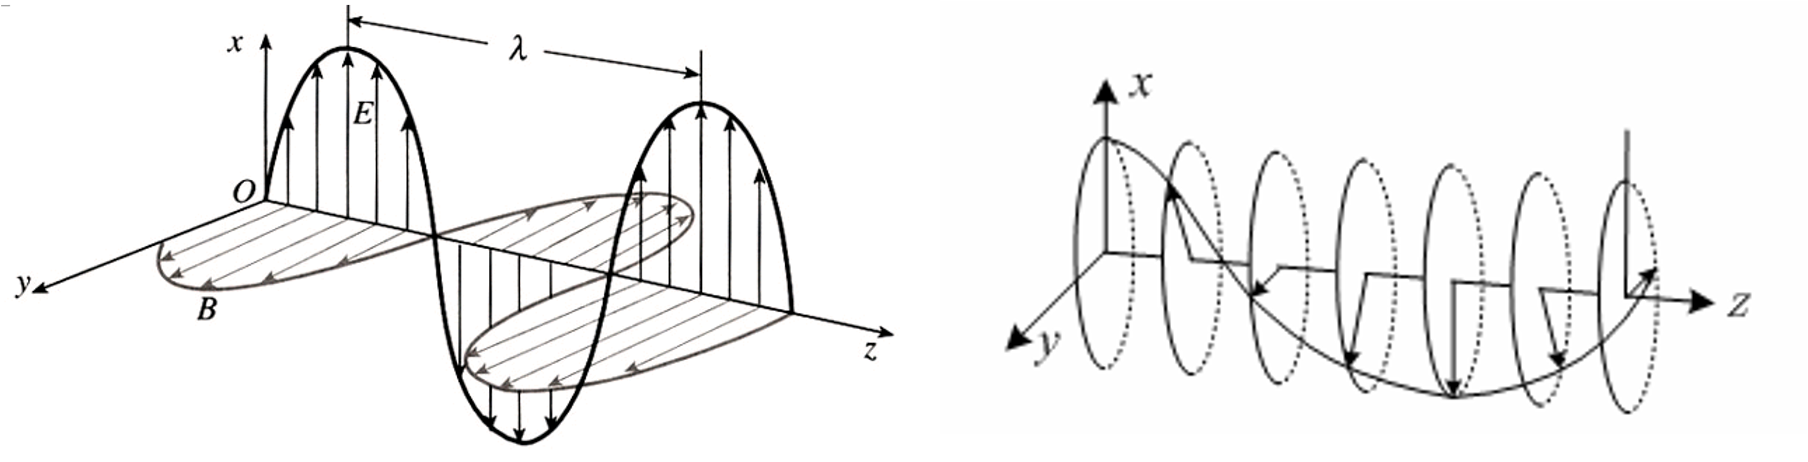
\includegraphics[width=0.8\textwidth]{figs/10.png}
   \end{center}
 考虑标量化.
 \begin{enumerate}
     \item 线偏振 $\mathbf{E}(z,t) = E_x(z,t) \hat{e}_x $ 
     \item 圆偏振 $\mathbf{E}(z,t) = E_x(z,t) \hat{e}_{\sigma}, \qquad \text{with} \qquad \hat{e}_{\pm}= \mp \frac{1}{\sqrt{2}} (\hat{x} \pm \hat{y}) $
 \end{enumerate}
\end{frame}

\begin{frame}
      \frametitle{}
      ~~\\
    \例 [1. 试求一维光学腔中的线偏振电磁场] {
      \begin{center}
           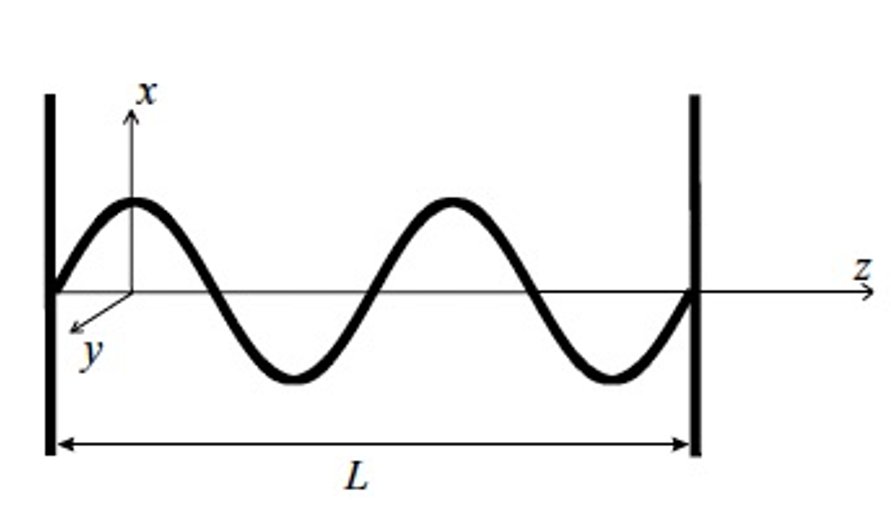
\includegraphics[width=0.4\textwidth]{figs/1.png}
      \end{center}  
      光学腔: $0\leq z\leq L$ \\  
      边界条件: $E_x(0)=E_x(L)=0$  
    }
    \解  设 $\displaystyle  E_x(z,t)=T(t)Z(z) $,代入波动方程 
    \[\mathbf{E}_{tt} =c^2\nabla^2 \mathbf{E}\]
\end{frame}

\begin{frame}
      \frametitle{} 
    得:
	\begin{equation*}
		 T~^{''}(t)Z(z) =c~^2 T(t)Z~^{''}(z) 
	\end{equation*}
	分离变量, 令: {\hspace*{2em}}
      $$ \dfrac{T~^{''}}{c~^2 T}=\dfrac{Z~^{''} }{Z} =-\lambda $$ \\ \vspace{0.3cm}
    转化为两常微分方程 \\ \vspace{0.3cm}
    方程(I):
      $\displaystyle  \begin{cases}
          Z~^{''} +\lambda Z=0  ~~,~~ 0<z<L\\
          Z(0)=0 ~,~Z(L)=0
      \end{cases}$ \\	
    方程(II):
      $\displaystyle  \begin{cases}
          T~^{''} +\lambda {c~^2 T}=0 \\
          ......
      \end{cases}$ \\	  
\end{frame}

\begin{frame}
      \frametitle{}
    特征(辅助)方程法解方程(I)  
    \begin{enumerate}
    \IItem 固有值:$\displaystyle  \lambda_n=\frac{n^2\pi^2}{L^2}= \omega^2 _n, \quad k_n=\frac{\omega_n}{c} $ 
    \IItem 固有解:$\displaystyle  E_n(z)=\sin (\omega_n z) $
    \end{enumerate}
    解方程II : 	\[ T~^{''} +\lambda {c~^2 T}=0 \] \\ 
	代入$\lambda_n$, 得:
	$\displaystyle  T~^{''} +\lambda~_n c~^2 ~T=0 $ \\
	变形为:\[  T~^{''} +\omega ~_n ^2 {c~^2 T}=0 \]
	特征方程有虚根,通解 :\\
	\hspace{3cm}	$\displaystyle 	T~_n=c~_n\cos \omega_n~c~t+ d~_n\sin \omega ~_n~c~t $  \\ \vspace{1em}
\end{frame}

\begin{frame}
    \frametitle{} 
    ~\\
    原方程的基本解:\\ {\vspace*{0.3em}}
	$\begin{array}{llll}
		E_n (z,t) &=& T_n(t)Z_n(z)\\
		&=& (c_n\cos \omega_nct+ d_n\sin \omega _nct ) \sin \omega_n z\\
        &=&a_n \exp(i \omega_n ct) \sin \frac{ n\pi z}{L} \\
	\end{array}$ \\  {\vspace*{0.6em}}    
    \begin{enumerate}
    %\IItem 基本解:$\displaystyle E_{n}(z,t) = a_n q_n (t) \sin (k_n z), \quad \text{with} \quad a_n = \left( \frac{2 \omega ^2}{V \epsilon_0}\right)^{1/2} $
    \IItem 基本解:$\displaystyle E_{n}(z,t) = a_n q_n (t) \sin (k_n z) $
    \IItem 叠加解:$\displaystyle E_{x}(z,t) = \sum\limits_{n=1}^{\infty } a_n q_n (t) \sin (k_n z)$
    \end{enumerate}	
    把解代回由麦克斯韦方程(III), 得磁场叠加解 \\ 
    \[ H_{y}(z,t) = \sum\limits_{n=1}^{\infty } a_n \frac{\epsilon_0}{k_n}q_n ' (t) \cos (k_n z)\] 
\end{frame}

\begin{frame}
      \frametitle{}
    令: 
    \[  L \to \infty \]
    得自由场解 
    \[  E_{x}(z,t) = \frac{1}{2} E_{0x}(z) \exp [i(kz-\omega t)] \]
    ~~\\ 
    电磁场的哈密顿(能量)
    \[ H = \frac{1}{2} \int_V d V \left[ \epsilon_0 \mathbf{E^2}(\mathbf{r},t) + \frac{1}{\mu_0}\mathbf{B^2}(\mathbf{r},t)\right]\]
\end{frame}

\begin{frame} 
\frametitle{波动光学基本结论}
    电磁场是一系列基本振动模式的叠加.\\ 
    \[ E_{x}(z,t) = \sum\limits_{n=1}^{\infty } a_n q_n (t) \sin (k_n z)\]
    \[ H_{y}(z,t) = \sum\limits_{n=1}^{\infty } a_n \frac{\epsilon_0}{k_n}q_n ' (t) \cos (k_n z)\] 
    自由场是自由振动;存在电荷或电流等环境,则是受迫振动, 波动方程为:
    \[\mathbf{E}_{tt} -c^2\nabla^2 \mathbf{E} = \mu_0 \frac{\partial ^2 \mathbf{P}  }{\partial t^2}\]  
\end{frame}

\begin{frame}
      \frametitle{经典光学面临的困难}
      基于麦克斯韦方程的波动光学, 不能解释如下实验
      \begin{itemize}
          \item 黑体辐射, 
          \item 光电效应, 
          \item 康普顿效应, 
          \item 原子光谱, 
          \item 光的发射与吸收...
      \end{itemize}
      * 对上述问题的解释导致量子力学的建立
\end{frame}

\section{2. 半经典光学}

\begin{frame}
      \frametitle{光量子假说}
      1900年, 普朗克提出热辐射能量子假说
      \[E= n \varepsilon , \qquad \varepsilon= h \nu= \hbar \omega\]
      1905年,爱因斯坦提出光量子假说, 揭示光的波粒二象性本质.  \\ {\vspace*{1em}}
      \[E= h \nu= \hbar \omega, \qquad  \mathbf{p}=\frac{h}{\lambda} \mathbf{n} = \hbar \mathbf{k} \]  
      \\  \vspace*{3em}

      基此发展出半经典光学, 可成功解释经典光学所面临的上述困难!
\end{frame}

\begin{frame}
    \frametitle{半经典光学}     
    \begin{itemize}
        \Item 量子化原子能级
        \Item 经典的光学场+光量子假说
    \end{itemize}  
\end{frame}

\begin{frame}
      \frametitle{}
      \例 [2. 试采用半经典方法处理光与原子的相互作用问题] {}
      \解~ 考虑沿z轴传播的单色光 
      \[ \left\{\begin{array}{l}
        E_{x}=E_{0} \cos \left(\frac{2 \pi}{\lambda} z-\omega t\right) \\
        E_{y}=E_{z}=0
        \end{array}\right. \]
     光与原子的相互作用发生在原子内部, 这个尺度的光场可认为是均匀场
     \[E_{x}=E_{0} \cos \left(\omega t\right)  \]
     光波所产生的能量可看做是对原子能级的微扰 
     \[\begin{aligned}
        &\hat{H}^{\prime}=e\mathbf{r}\cdot\mathbf{E}  = ex E_{x} \\
        &=\frac{1}{2} \operatorname{ex} E_{0}\left[e^{i \omega t}+e^{-i \omega t}\right] \\
        &=\hat{F}\left[e^{i \omega t}+e^{-i \omega t}\right]
        \end{aligned}
      \]
\end{frame}

\begin{frame}
      \frametitle{}
      代入含时微扰公式
      \[ \omega_{m \rightarrow k}=\frac{2 \pi}{\hbar}\left|F_{k m}\right|^{2} \delta\left(\varepsilon_{k}-\varepsilon_{m}+\hbar \omega\right) \]
      对于自然光,可得跃迁概率:
      \[ w_{k \rightarrow m}=\frac{4 \pi^{2} e^{2}}{3 \hbar^{2}} I\left(\omega_{m k}\right)\left|\vec{r}_{m k}\right|^{2} = B_{km} I\left(\omega_{m k}\right)\]
      求得爱因斯坦吸收系数 $B_{km}$ \\ 
      同理,得爱因斯坦受激发射系数 $B_{mk}$  \\ 
      代入电磁辐射平衡条件(发射的光子数等于吸收的光子数) 
      \[N_{m}\left[A_{m k}+B_{m k} I\left(\omega_{m k}\right)\right]=N_{k} B_{k m} I\left(\omega_{m k}\right) \]
      得自发发射系数 $A_{mk}$ 
\end{frame}

\begin{frame}
      \frametitle{}
      基于光子数目决定电磁场强度的基本假设, 得辐射场强度
    \[\begin{aligned}
        J_{m k} &=N_{m} A_{m k} \hbar \omega_{m k} \\
        &=N_{m} \frac{4 e^{2} \omega_{m k}^{4}}{3 c^{3}}\left|\vec{r}_{k m}\right|^{2} 
        \end{aligned} \] {\vspace*{2.3em}}
    成功解决辐射场问题, 如: 选择定则, 激发态寿命, 常见光谱, ... \\ \vspace*{2.0em}
    增加自旋, 解决光谱分裂问题 \\
    增加旋-轨耦合,解决复杂光谱问题 \\ 
    增加非线性效应,解决变频问题 \\
\end{frame}

\begin{frame}
    \frametitle{半经典光学面临的困难}
    半经典半量子光学取得了具大成功. \\ 
    但不能解释如下光学现象
    \begin{itemize}
        \item 延迟选择实验
        \item 量子擦除实验
        \item 相干态
        \item 压缩态
        \item 纠缠光子对
        \item 单光子源
        \item 量子隐形传态
    \end{itemize}
    * 这些问题的解释导致第二次量子革命, 1956年后, 发展出非经典光源 (激光, 压缩光, 单光子), 人类进入量子光学时代.
\end{frame}

\begin{frame}
    \frametitle{惠勒延迟选择实验}
    \begin{center}
        \includegraphics[width=0.6\textwidth]{figs/choose.png} \\
    \end{center} 
    {\Bullet} 光子总是处于叠加
    {\Bullet} 光路的说法是不成立的
\end{frame}

%\begin{frame}
%    \frametitle{量子擦除实验}
%    \begin{center}
%        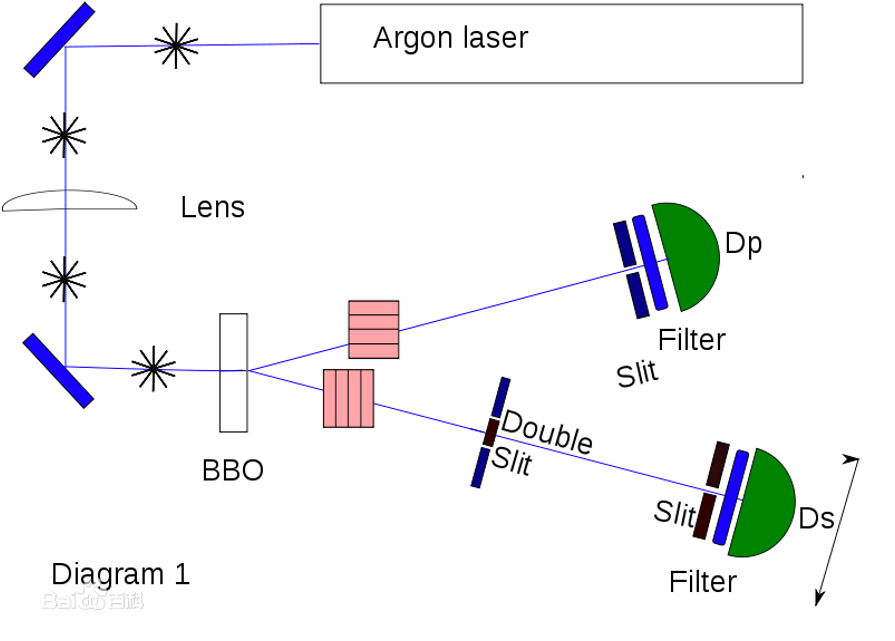
\includegraphics[width=0.6\textwidth]{figs/c1.%png} \\
%    \end{center} 
%\end{frame}
%
%\begin{frame}
%    \frametitle{}
%    \begin{center}
%        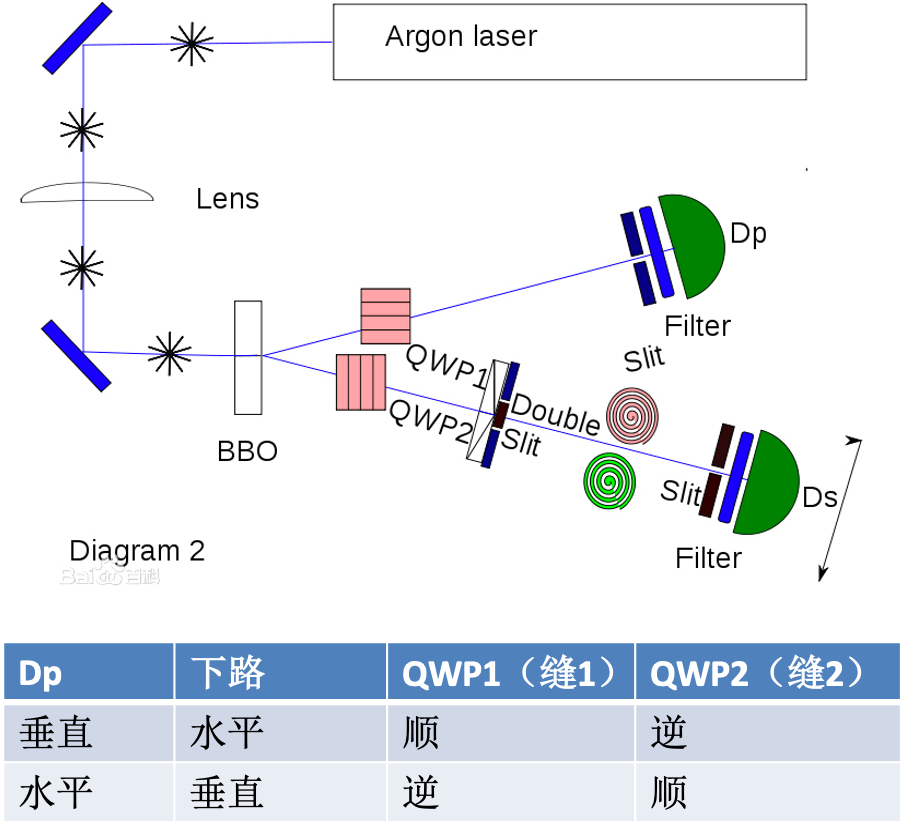
\includegraphics[width=0.6\textwidth]{figs/c2.%png} \\
%    \end{center} 
%\end{frame}
%
%\begin{frame}
%    \frametitle{}
%    \begin{center}
%        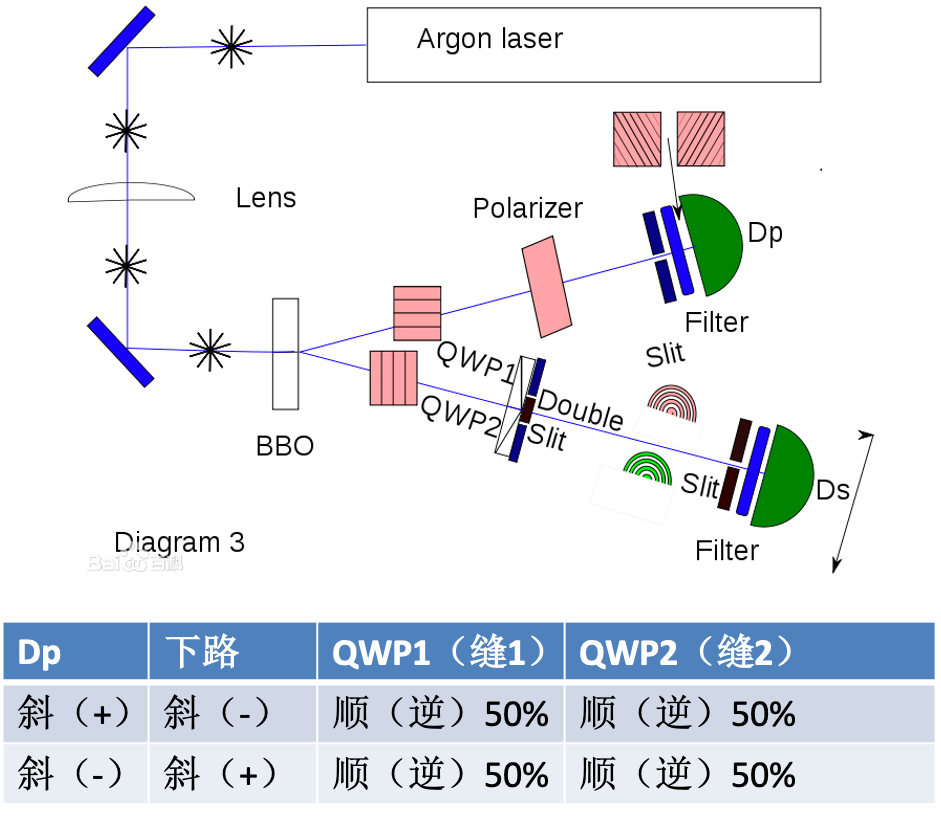
\includegraphics[width=0.6\textwidth]{figs/c3.%png} \\
%    \end{center} 
%\end{frame}

%%%%%%%%%%%%%%%%%%%%%%%%%%%%%%%%%%%%%%%%%%%%%%%%%%%%%%%%%%%%%%%%%%%
\begin{frame}
    \frametitle{课外作业}
    \begin{enumerate}
        \item 补全例1的计算
        \item 补全例2的计算
        \item 了解非线性光学
        \item 量子擦除实验说明什么?
    \end{enumerate}
\end{frame}
%%%%%%%%%%%%%%%%%%%%%%%%%%%%%%%%%%%%%%%%%%%%%%%%%%%%%%%%%%%%%%%%%%%

        % 半经典光
%
\begin{frame}
    \frametitle{前情回顾}
    学习量子光学的必要性
    \begin{itemize}
        \Item 经典光学(麦克斯韦方程) \\
        <-> 黑体辐射, 光电效应, 康普顿效应, 原子光谱, 自发发射, 受激发射...
        \Item 半经典光学(量子化粒子+经典光场)  \\
        <-> 延迟选择实验, 量子擦除实验, 相干态, 压缩态, 量子计算, 量子通信, 量子存储...
        \Item 量子光学(量子化粒子+量子化光场)   
    \end{itemize}     
\end{frame}

\begin{frame}
    \frametitle{场与粒子}
    物理学基本认识:
    \begin{itemize}
        \item 场是物质存在的基本形式
        \item 所有的粒子都是场的量子
        \item 场量子与量子力学的粒子并不完全一样,在非相对论近似下两者可拟合在一起
        \item 光量子是光场的量子,无非相对论近似,不是量子力学中的粒子
    \end{itemize} 
\end{frame}

%%%%%%%%%%%%%%%%%%%%%%%%%%%%%%%%%%%%%%%%%%%%%%%%%%%%%%%%%%%%%
\begin{frame} [plain]
    \frametitle{}
    \Background[1] 
    \begin{center}
    {\huge 第2-3讲:量子力学基础}
    \end{center}  
    \addtocounter{framenumber}{-1}   
\end{frame}
%%%%%%%%%%%%%%%%%%%%%%%%%%%%%%%%%%%%%%%%%%%%%%%%%%%%%%%%%5%%%

\section{1.量子态与希尔伯特空间}

\begin{frame} 
    \frametitle{希尔伯特空间}
    量子态用希尔伯特空间的矢量描述\\
    \begin{equation*}
        \begin{split}
            \text{1、定义加法} \quad  &\xi=\psi+\varphi\\
            &\psi+\varphi=\varphi+\psi \qquad (\text{交换律})\\
            &(\psi+\varphi)+\xi=\psi+(\varphi+\xi) \qquad (\text{结合律})\\
            &\psi+\text{O}= \psi \qquad (\text{零元})\\
            &\psi+\varphi= \text{O} \qquad (\text{逆元})\\
        \end{split}  
    \end{equation*}
\end{frame} 

\begin{frame} 
    \begin{equation*}
        \begin{split}
            \text{2、定义数乘} \quad &\varphi=\psi a\\
            &\psi 1= \psi \qquad (\text{1元})\\
            &(\psi a)b=\psi (ab) \qquad (\text{结合律})\\
            &\psi(a+b)= \psi a+ \psi b \qquad (\text{第一分配律})\\
            &(\psi+\varphi) a= \psi a +\varphi a \qquad (\text{第二分配律})\\
        \end{split}  
    \end{equation*}
\end{frame} 

\begin{frame} 
    \begin{equation*}
        \begin{split}
            \text{3、定义内积} \quad &c=(\psi, \varphi)\\
            &(\psi, \varphi)= (\varphi,\psi)^* \\
            &(\psi, \varphi+\xi)= (\psi, \varphi) + (\psi, \xi)\qquad (\text{分配律})\\
            &(\psi, \varphi a)= (\psi, \varphi )a \\
            &(\psi a, \varphi )= a^* (\psi, \varphi ) \\
            &(\psi,\psi)= c\ge 0\\
        \end{split}  
    \end{equation*}
\end{frame}

\begin{frame} 
    \例 [0. 有定义在$C^n$空间的列矩阵,求内积]
    { \[\psi=
        \begin{pmatrix}
                a_1\\
                a_2\\
                a_3
        \end{pmatrix}, \qquad 
        \varphi =\begin{pmatrix}
            b_1\\
            b_2\\
            b_3
    \end{pmatrix}
     \] 
    }
    \解 ~ \[(\psi, \varphi) = \begin{pmatrix}
        a_1 ^* &
        a_2 ^* &
        a_3 ^*
    \end{pmatrix}
        \begin{pmatrix}
        b_1\\
        b_2\\
        b_3
    \end{pmatrix}
    =a_1 ^* b_1 +a_2 ^* b_2 +a_3 ^* b_3
    =c 
    \]
    ~ \[(\varphi,\psi) = \begin{pmatrix}
        b_1 ^* &
        b_2 ^* &
        b_3 ^*
    \end{pmatrix}
        \begin{pmatrix}
        a_1\\
        a_2\\
        a_3
    \end{pmatrix}
    =b_1 ^* a_1 +b_2 ^* a_2 +b_3 ^* a_3
    =c^* 
    \]
\end{frame} 

\begin{frame} 
    \例 [1. 求定义在x空间的函数的内积]{}

    \解 ~ \[(\psi, \varphi)=\int_a ^b \psi^*(x)  \varphi(x) dx =c\]
    \[(\varphi,\psi)=\int_a ^b \varphi^*(x)\psi(x) dx = (\int_a ^b \varphi(x)\psi^*(x) dx) ^* =c^*\]
\end{frame} 

\begin{frame}
    4、定义空间\\
   \begin{itemize}
       \Item 矢量空间:满足加法和数乘两种运算的集合
       \Item 内积空间:满足加法、数乘和内积三种运算的集合
       \Item 希尔伯特空间:  完全的内积空间\\
       ~~ \\
       *完全性:对给定任意小的实数$\varepsilon$,总有数N存在,当m, n>N时,有\\
       $$ (\psi_m -\psi_n, \psi_m -\psi_n )< \varepsilon $$
   \end{itemize} 
   \Tips ~ 量子体系的状态用希尔伯特空间的矢量描述
\end{frame} 

\begin{frame}
    5、几个概念\\
   \begin{itemize}
       \Item 模(方):$|\psi|^2= (\psi, \psi)=c$
       \Item 归一化: $|\psi|^2= (\psi, \psi)=c=1$
       \Item 正交性(线性无关):  $(\psi, \varphi)=0 $ \\
       \Item 完全集: 有一组线性无关集,如果空间的任意矢量都可以在其上展开,则称它为一个完全集,记为$\{\phi_i\}$
       \[\psi=\sum_i a_i \phi_i= \sum_i (\phi_i,\psi) \phi_i\]
       \Item 维度:最小完全集所包含矢量的数目相同,称这个数目为空间的维度
       \Item 正交归一完全集:对于一个n维的完全集,有:\[(\phi_i,\phi_j)=\delta_{ij}, \qquad i,j=1,2,3,\cdots, n \]
       \Item 基与基矢:称一个正交归一完全集为空间的一个基,它所含的矢量称不计算基矢
   \end{itemize} 
\end{frame} 

\begin{frame}
 \Tips~ 同一空间可以有不同的基,\\
 $C^2$空间的一个基:
 \[ \rs{0}\equiv\begin{bmatrix}
     1 \\
     0
 \end{bmatrix}; \qquad \rs{1}\equiv\begin{bmatrix}
    0 \\
    1
\end{bmatrix} \]

$C^2$空间的另一个基:
\[ \rs{+}\equiv\frac{1}{\sqrt{2}}\begin{bmatrix}
    1 \\
    1
\end{bmatrix}=\Pstate; \qquad \rs{-}\equiv\frac{1}{\sqrt{2}}\begin{bmatrix}
   1 \\
   -1
\end{bmatrix}=\Mstate \]
它们可以相互转换.
\end{frame} 

\begin{frame} 
    例: 若$\rs{0}, \rs{1}$描述垂直和水平偏振, 则 $\rs{+}, \rs{-}$ 描述正负45度偏振. 
    \begin{center}
        \begin{overpic} [width=0.7\textwidth]{figs/26.png}
            %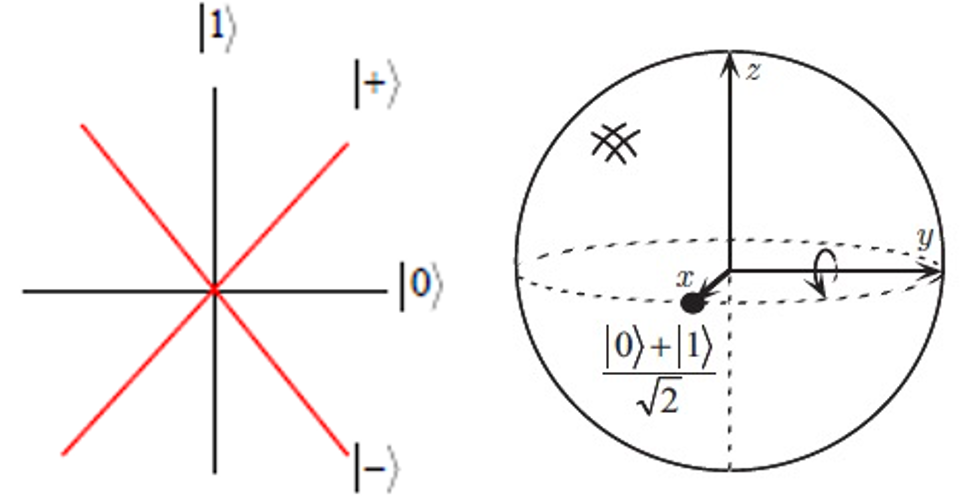
\includegraphics[width=0.7\textwidth]{figs/26.png}
            \put(72,48){\small\bfseries \color{red}{$|1\rangle$}}
            \put(72,-1){\small\bfseries \color{red}{$|0\rangle$}}
        \end{overpic}   
    \end{center} 
    若$\rs{0}, \rs{1}$描述在Z方向自旋投影, 则 $\rs{+}, \rs{-}$ 描述在X方向的自旋投影. 
\end{frame}

\begin{frame}{}
    6、左矢与右矢\\
    考察内积: $(\psi,\psi)=\int\psi^*\psi d\tau$ \\
    同一波函数放在左边还是右边,意义有所不同: \\
    右边是线性的:  $(\psi,a\psi)=(\psi,\psi)a $ \\
    左边是反线性的:   $(a\psi,\psi)=a^* (\psi,\psi)$  \\
    为清楚描述线性反线性特点,定义左矢和右矢, 写狄拉克记号
    $$\langle \psi |, \qquad |\psi \rangle $$ 
    数乘性质: $$\langle a\psi | = \langle \psi |a^* $$
    $$ |a\psi \rangle = a|\psi \rangle$$ 
    内积:\[(\psi,\varphi)\equiv \langle \psi | \varphi \rangle\]
\end{frame}

\begin{frame}{}
    7、外积\\
    考察展开式: \[\psi=\sum_i a_i \phi_i= \sum_i (\phi_i,\psi) \phi_i\]
    \[\rs{\psi}=\sum_i a_i \rs{\phi_i}= \sum_i \lr{\phi_i}{\psi} \rs{\phi_i} =\sum_i \rl{\phi_i}{\phi_i} \rs{\psi}\]
    ~~\\
    令 $p_i= \rl{\phi_i}{\phi_i} $, 称为外积\\ {\vspace*{1em}}
    完备性:
    \[\sum_i p_i= \sum_i \rl{\phi_i}{\phi_i}=1 \]
\end{frame}

\begin{frame}{}
        \例 [2. 有定义在$C^n$空间的列矩阵,求内积和外积]
        { \[\rs{\psi}=
            \begin{pmatrix}
                    a_1\\
                    a_2\\
                    a_3
            \end{pmatrix}, \qquad 
            \rs{\varphi} =\begin{pmatrix}
                b_1\\
                b_2\\
                b_3
        \end{pmatrix}
         \] 
        }
        \解 ~ \[\lr{\psi}{\varphi} = \begin{pmatrix}
            a_1 ^* &
            a_2 ^* &
            a_3 ^*
        \end{pmatrix}
            \begin{pmatrix}
            b_1\\
            b_2\\
            b_3
        \end{pmatrix}
        =a_1 ^* b_1 +a_2 ^* b_2 +a_3 ^* b_3
        =c 
        \]
        ~ \[\rl{\psi}{\varphi} = \begin{pmatrix}
            a_1  \\
            a_2  \\
            a_3 
        \end{pmatrix}
            \begin{pmatrix}
            b_1 ^* &
            b_2 ^* &
            b_3 ^*
        \end{pmatrix}
        =  \begin{pmatrix}
            a_1b_1 ^* & a_1b_2 ^* & a_1b_3 ^* \\
            a_2b_1 ^* & a_2b_2 ^* & a_2b_3 ^* \\
            a_3b_1 ^* & a_3b_2 ^* & a_3b_3 ^* 
        \end{pmatrix}
        \]
\end{frame}

\begin{frame} 
\frametitle{}
 \例 [3. 求如下波函数的外积]{
 \[\rs{\psi}= a_1 \rs{1} + a_2 \rs{2}, \quad \rs{\varphi}= b_1 \rs{1} + b_2 \rs{2} \]}
 \解 ~(1) 代数形式 
   \[ \begin{aligned}
    \rl{\psi}{\varphi} &= (a_1 \rs{1} + a_2 \rs{2}) (\ls{1}b_1 ^*  + \ls{2} b_2 ^* )\\
      &= a_1 b_1 ^* \rl{1}{1} + a_2 b_2 ^* \rl{2}{2} + a_1 b_2 ^* \rl{1}{2} + a_2 b_1 ^* \rl{2}{1} \\
   \end{aligned}\]   
* 后两项为耦合项\\ 
(2) 矩阵形式
~ \[\rl{\psi}{\varphi} = \begin{pmatrix}
    a_1  \\
    a_2  
\end{pmatrix}
    \begin{pmatrix}
    b_1 ^* &
    b_2 ^* &
\end{pmatrix}
=  \begin{pmatrix}
    a_1b_1 ^* & a_1b_2 ^*  \\
    a_2b_1 ^* & a_2b_2 ^*  
\end{pmatrix}
\]
* 非对称元为耦合项
\end{frame}

\section{2.物理量与算符}

\begin{frame}
    \frametitle{算符}
    物理量用希尔伯特空间的线性厄密算符描述\\
    1. 定义:
    \begin{itemize}
        \Item 算符:描述态矢量之间的映射关系,算符作用于一个态映射到另一态。
        \[F \rs{\Psi}=\rs{\psi}\]
        \Item 算符相等: 对任意态$\rs{\psi}$, 恒有下式, 则 $A= B$ \[ A\rs{\psi}=B\rs{\psi}\]
        \Item 单位算符: \[I\Psi=\Psi \]
        \Item 算符的和:  
        $$ (A+B)\Psi=A\Psi+B\Psi $$   
    \end{itemize}
\end{frame} 

\begin{frame}
 \frametitle{}
 \begin{itemize}
    \Item 算符的积 
    $$ (AB)\Psi=A(B\Psi) $$
    * 不存在交换律,即 $AB=BA$ 或 $AB\ne BA$ 皆有可能 \\
    定义对易子来描述 \\
    $$ [A,B]=AB-BA$$
    若[A,B]=0,称两算符对易(可交换),否则不对易(不可交换)
    \Item 逆算符  
    \[F^{-1}\rs{\psi}=\rs{\Psi} \] 
    \Item 线性算符 \[F (a\rs{\Psi} +b\rs{\psi}) = aF \rs{\Psi} +bF\rs{\psi}\]
\end{itemize}
\end{frame}

\begin{frame}
    \frametitle{}
    \begin{itemize}
        \Item 伴算符   \[\ls{\psi}=\ls{\Psi}F^{\dagger} \]
        \[F^{\dagger} = (F^* _{nm})^T \]
        \Item 自伴(厄密)算符  \[F = F^{\dagger} \] 
        性质(1): $\lr{\Psi F}{\psi}=\lr{\Psi }{F \psi}=\lcr{\Psi }{F} {\psi}$ \\
        性质(2): $\lcr{\Psi }{F} {\psi}=\lcr{\psi }{F} {\Psi}^*$ \\ \vspace{0.6em}
        \Item 幺正(酉)算符    \[F^{-1} = F^{\dagger} \] 性质: $FF^{\dagger}=F^{\dagger}F=I$, 通常写成 $UU^{\dagger}=U^{\dagger}U=I$ \\ \vspace{1.0em}
    \end{itemize}        
\end{frame}

\begin{frame}
    \frametitle{}
    \Tips 幺正(酉)变换实现空间变换: 把一个空间所有矢量都用同一幺正算符作用,得到的另一个新的空间,
    \[U\rs{\Psi} =\rs{\Psi'}\]
    {\Bullet}~新旧空间算符之间的关系: \\
        旧空间的算符: \[F \rs{\Psi}=\rs{\varphi}\]
        新空间的算符: \[F' \rs{\Psi'}=\rs{\varphi'}\]
        关系:
        \[F' U\rs{\Psi}=U\rs{\varphi}\]
        \[F' U\rs{\Psi}=UF \rs{\Psi}\]
        \[U^{\dagger}F' U\rs{\Psi}=U^{\dagger}UF \rs{\Psi}\]
        \[U^{\dagger}F' U=F \]
\end{frame}

\begin{frame}
    \frametitle{}
    \begin{itemize}
    \Item 投影算符: 基矢的外积是一种投影算符,
    \end{itemize}
    对于展开式: 
    \[\rs{\psi}=\sum_i a_i \rs{\phi_i}=\sum_i \rs{\phi_i} \lr{\phi_i}{\psi}=\sum_i p_i \rs{\psi} =\sum_i \rs{\psi_i}\]
    有:\[p_i \rs{\psi} =\rs{\psi_i}\]
    即,外积$\rl{\phi_i}{\phi_i}$作用于$\rs{\psi}$,得到第$i$个基矢态上的投影分量!\\
\end{frame}

\begin{frame}    
    \begin{itemize}
        \Item 测量算子: 常称投影算符为测量算子. 对于$C^2$空间, 定义为:
        \end{itemize}
    \[M_0=\rl{0}{0}, \qquad M_1=\rl{1}{1} \]
    具有$2\times 2$的矩阵形式,
    可以证明:\\
    {\bullet} 测量算子是自伴(厄密)算符 :\[M_m = M_m ^{\dagger} \]
    {\bullet} 平方不变性 :\[M_m ^2 = M_m \]
    {\bullet} 完备性 :\[M_0 + M_1 = M_0 ^2 + M_1 ^2 = M_0 M_0 ^\dagger + M_1 M_0 ^\dagger=I\]
\end{frame}

\begin{frame} 
    \frametitle{}
    {\bullet} 测量后的态函数 
    \[\begin{aligned}
        M_0\rs{\Psi} 
        &= \rl{0}{0}(a_0\rs{0}+a_1\rs{1})  \\ 
        &= \rl{0}{0}a_0\rs{0}  \\ 
        &= a_0\rs{0}  \\ 
        &= \frac{a_0}{|a_0|}\rs{0}  \qquad \text{(归一化)} \\ 
    \end{aligned}\]    
    {\bullet} 测得的概率(密度) 
    \[\begin{aligned}
        \lcr{\Psi}{M_0 ^\dagger M_0}{\Psi} 
        &= \lcr{0 }{a_0 ^* a_0} {0} \\ 
        &= \lr{0 }{0}a_0 ^* a_0 \\ 
        &= |a_0|^2 = p(0) 
    \end{aligned}\] 
    重写测量后的状态 \[  M_m\rs{\Psi} = \frac{a_m\rs{m}}{\sqrt{\lcr{\Psi}{M_m ^\dagger M_m}{\Psi}}} = \frac{M_m\rs{\Psi}}{\sqrt{\lcr{\Psi}{M_m ^\dagger M_m}{\Psi}}}\]
\end{frame}

\begin{frame}
    \frametitle{}
    ~\\
    2. 算符的代数形式 \\ {\vspace*{0.3em}}
 {\Bullet}位置算符和动量算符
\例[4.已知粒子的位置波函数$\psi(x,t)$,求动量的期望值]{}   
\解~ 由概率诠释,位置期望值为
\begin{equation*}
    \bar{x}=\int x|\psi(x, t)|^{2} d x=\int \psi^{*}(x, t) x \psi(x, t) d x
\end{equation*}
对于动量波函数 $c(p,t)$, 动量期望值为
\begin{equation*}
    \bar{p_x}=\int p_x|c(p_x, t)|^{2} d p_x=\int c^{*}(p_x, t) p c(p_x, t) d p_x
\end{equation*}
很明显,有
\begin{equation*}
    \bar{p_x}\neq\int p_x|\psi(x, t)|^{2} d p_x
\end{equation*}
\end{frame} 

\begin{frame}
变换求解
\begin{equation*}
    \begin{split}
        \bar{p}&=\int c^{*}(p) p c(p) d p \\  
        &=\int (\frac{1}{\sqrt{2 \pi \hbar}} \int \psi^{*}(x) e^{\frac{i}{\hbar} p\cdot x} d x) p c\left(p\right) d p \\
        &=\frac{1}{\sqrt{2 \pi \hbar}} \int \int \psi^{*}(x) (e^{\frac{i}{\hbar} p\cdot x}  p) c\left(p\right) d xd p \\
        &=\frac{1}{\sqrt{2 \pi \hbar}} \int \int \psi^{*}(x) \Myitem{t1}{red}{(-i\hbar\frac{d}{d x} e^{\frac{i}{\hbar} p\cdot x})} c(p) d xd p \\
        &=\int \psi^{*}(x) (-i\hbar\frac{d}{d x}) (\frac{1}{\sqrt{2 \pi \hbar}} \int e^{\frac{i}{\hbar} p\cdot x} c(p) d p)  d x\\
        &=\int \psi^{*}(x) (-i\hbar\frac{d}{d x}) \psi(x)  d x\\
     \end{split}
\end{equation*}  
\end{frame} 

\begin{frame}
定义如下计算符号:
$$ \boxed{\hat{p}_x= -i\hbar\frac{d}{d x}} $$ 
上式变为:         
$$\boxed{\bar{p}_x=\int \psi^{*}(x) \hat{p}_x \psi(x) d x} $$
称$ \hat{p}_x= -i\hbar\dfrac{d}{d x} $ 为位置表象里的动量算符表示($p_x$分量)\\
同理,称 $\hat{x}= x $ 为位置表象里的位置算符表示($x$分量)\\ \vspace{0.3em}
存在量子力学基本对易关系 \[ [\hat{x},\hat{p}_x]=i\hbar\] 
\end{frame}

\begin{frame} 
    \frametitle{}
    {\Bullet} 任意力学量的算符
    \begin{tcolorbox1}{命题:}
    已知位置、动量的算符表示如下,
    \begin{itemize}
        \Item  位置算符(三维): $ \hat{\vec{r}} =\vec{r} $
        \Item  动量算符(三维): $ \hat{\vec{p}} =-i\hbar(\dfrac{d}{d x}, \dfrac{d}{d y} , \dfrac{d}{d z})=-i\hbar \nabla $
    \end{itemize}
    求任意其他力学量的算符
    \end{tcolorbox1}
    \alert{Bohm规则(1):} 经典物理学的力学量F,若是位置与动量的函数
    \[F(\vec{r},\vec{p})\]
    则其量子力学算符为:
    \[\hat{F}=F(\hat{\vec{r}},\hat{\vec{p}})\]
\end{frame} 

\begin{frame}
    \frametitle{}     
{\Bullet}正则位置和正则动量
  \[ \frac{\mathrm{d }q}{\mathrm{d }t} = \frac{\partial H(q,p) }{\partial p}, \quad \frac{\mathrm{d }p}{\mathrm{d }t} = -\frac{ \partial H(q,p) }{\partial q} \]
  正则位置和正则动量算符的对易关系
  \[ [\hat{q},\hat{p}]=i\hbar\]
  \alert{Bohm规则(2):} 经典物理学存在力学量F,是正则位置与动量的函数
  \[F(q,p)\]
  则其量子力学算符为:
  \[\hat{F}=F(\hat{q},\hat{p})\]
  量子涨落关系(不确定性原理) \[\overline{(\Delta \hat{q})^2} \cdot \overline{(\Delta \hat{p})^2} \geq  \frac{1}{4} \hbar ^2 \]
\end{frame} 

\begin{frame}
    \frametitle{}
    3. 算符的矩阵形式
    \[\begin{aligned}
        \rs{\psi}&=F \rs{\Psi} \\
        \lr{i}{\psi}&= \lcr{i}{F}{\Psi} \\
        \lr{i}{\psi}&= \sum_j\lcr{i}{F}{j}\lr{j}{\Psi} \\
        \lr{i}{\psi}&= \sum_j F_{ij}\lr{j}{\Psi}
    \end{aligned}\]  
    算符矩阵元公式:\[ F_{ij}=\lcr{i}{F}{j}\]
    伴算符的矩阵等于原算符的厄密共轭:\[ F^{\dagger}=(F_{ij} ^*)^T\]
\end{frame}

\begin{frame}
    \frametitle{}
    4. 算符的本征方程
    \begin{itemize}
        \Item 定义式: \[F \rs{n}=f_n\rs{n}\]
        \Item 相关定理:
        \begin{itemize}
            \IItem 厄密算符的本征值是实数
            \IItem 厄密算符的所有本征矢构成正交归一完全集
            \IItem 当且仅当两厄密算符互相对易时才俱有共同的本征矢完全集
            \IItem 完全确定一个量子态所需要的彼此对易的一组力学量算符的最小集称为力学量完全集,所含力学量数目与体系的自由度数目相同
            \end{itemize}
    \end{itemize}
\end{frame}

\section{3.狄拉克记号量子力学}

\begin{frame} 
    \frametitle{狄拉克记号的量子力学}  
    量子态(无表象): $\hspace{1em}|\Psi \rangle, \quad$ 位置表象:$\hspace{1em} \langle x |\Psi \rangle , \quad$ 动量表象:$\hspace{1em} \langle p_x |\Psi \rangle$ \\ \vspace{0.1em}
    算符: $F, \quad$ 位置表象:$\hspace{1em} F(x, -i\hbar \frac{\partial }{\partial x}) , \quad$ 动量表象:$\hspace{1em} F(i\hbar \frac{\partial }{\partial p_x}, p_x) $ \\ \vspace{0.1em}
    展开式: $\hspace{1em}|\Psi \rangle =\sum\limits_{n=1} ^n a_n |n \rangle$ \\
    内积:   $\hspace{2em}\langle \varphi | \Psi \rangle = (\varphi, \Psi)= \int \varphi^*\Psi d\tau $ \\  \vspace{0.1em}
    归一化: $\hspace{1em}\langle \Psi | \Psi \rangle = (\Psi, \Psi)= \int \Psi^*\Psi d\tau = 1 $ \\ \vspace{0.1em}
    正交归一: $\langle n | m \rangle = \delta_{nm} $ \\ \vspace{0.1em}
    $ \hspace{5em} \langle \lambda | \lambda' \rangle = \delta(\lambda-\lambda') $\\ \vspace{0.2em}
    展开系数: $ a_n= \langle n | \Psi \rangle$ \\ \vspace{0.2em}
    展开系数: $ a_n ^*= \langle \Psi | n \rangle$ \\ \vspace{0.2em}
\end{frame} 
 
\begin{frame} 
    平均值:  $\hspace{1em}\bar{F} = \langle \Psi |F | \Psi \rangle$ \\ \vspace{0.2em}
    矩阵元:  $\hspace{1em}F_{nm} = \langle n |F | m \rangle$ \\ \vspace{0.2em}
    幺正变换:$S_{m\alpha} =\langle m| \alpha \rangle $ \\ \vspace{0.2em}
    投影算符:$p_i = |i\rangle\langle i |, \quad \text{封闭性:} \sum_i |i\rangle\langle i |=1 $ \\ \vspace{0.2em}
    本征方程:$F|n\rangle =f_n |n\rangle$ \\ \vspace{0.2em}
    薛定谔方程:$$ i\hbar \frac{\partial }{\partial t} |\Psi(t)\rangle = H|\Psi(t)\rangle $$ 
    算符运动方程:$$ \frac{d\bar{A}(t)}{dt}=\overline{(\frac{\partial A(t) }{\partial t})}  +\frac{1}{i\hbar} \overline{[A(t),H(t)]}$$
\end{frame} 

\begin{frame} 
    \例 [求薛定谔方程在各表象中的形式]{} 
    $$ \begin{aligned}
    i \hbar \frac{\partial}{\partial t} |\Psi(t) \rangle &= H |\Psi(t) \rangle  , \quad \text{无表象}\\
    i \hbar \frac{\partial}{\partial t} \langle x|\Psi(t) \rangle &= H (x, \hat{p}_x) \langle x|\Psi(t) \rangle  , \quad \text{位置表象}\\
    i \hbar \frac{\partial}{\partial t} \langle x|\Psi(t) \rangle &= [- \frac{\hbar^2}{2\mu} \frac{\partial ^2 }{\partial x^2} + U(x)] \langle x|\Psi(t) \rangle  , \quad \text{位置表象}\\
    i \hbar \frac{\partial}{\partial t} \langle p_x|\Psi(t) \rangle &= H (\hat{x}, p_x) \langle p_x|\Psi(t) \rangle  , \quad \text{动量表象}\\
    i \hbar \frac{\partial}{\partial t} \langle p_x|\Psi(t) \rangle &=  [ \frac{p^2 _x}{2\mu} + U(i \hbar \frac{\partial }{\partial p_x}) ] \langle p_x|\Psi(t) \rangle  , \quad \text{动量表象}\\
    i \hbar \frac{\partial}{\partial t} \langle n|\Psi(t) \rangle &=  \langle n|H|m \rangle \langle n |\Psi(t) \rangle  , \quad \text{Q表象}\\
    \end{aligned}
    $$
\end{frame} 

\begin{frame} 
 \frametitle{密度算符}
    
    设系统以$P_i$的概率出现$\rs{\psi_i}$ 态上, 求物理量F的平均值:\\ 
    (1) 物理量F在$\rs{\psi_i}$的均值
    \[\overline{F_i}=\ls{\psi_i}F \rs{\psi_i}
    \]
    (2) 测得$\overline{F_i}$的概率为$P_i$,所以均值为
    \[\overline{F}= \sum_i P_i \overline{F_i}\]
\end{frame}

\begin{frame} 
 \frametitle{} ~\\
      \例 [5. 若物体处于纯态, 即其状态能用一个态矢量$\rs{\psi}$描述, 求物理$F$的平均值] {
      \[ \begin{aligned}
          \overline{F} &= \lcr{\psi}{F}{\psi} \\
          &= \sum_n \lcr{\psi}{F}{n}\lr{n}{\psi}   \\
          &= \sum_n \lr{n}{\psi} \lcr{\psi}{F}{n} \\ 
          &=  \sum_n \lcr{n}{\rho F}{n} \\
          &= Tr (\rho F)
      \end{aligned}\] }
    式中定义了纯态$\rs{\psi}$的密度算符:
    \[\rho = \rl{\psi}{\psi}  \]
\end{frame}

\begin{frame} 
 \frametitle{}
 ~\\
 \例 [5'. 若物体处于混态,则要用一系列场矢量\{$\rs{\psi_i}$\}描述. 设测量其处于$\rs{\psi_i}$的概率为$P_i$, 求物理$F$的平均值] { 
      \[ \begin{aligned}
        \overline{F} &= \sum_i P_i \overline{F_i}\\
        &= \sum_i P_i \ls{\psi_i}F \rs{\psi_i} \\ 
        &= \sum_i P_i \sum_n \lcr{\psi_i}{F}{n}\lr{n}{\psi_i} \\
        &= \sum_n\ls{n} (\sum_i P_i \rl{\psi_i}{\psi_i} )F \rs{n} \\ 
        &= \sum_n\ls{n} \rho F\rs{n} = Tr (\rho F)
      \end{aligned}\] } 
      式中定义了混态的密度算符:
      $\rho = \sum_i P_i\rl{\psi_i}{\psi_i} $ 
\end{frame}

\begin{frame} 
 \frametitle{密度算符的性质}
 用密度算符求平均值, 纯态与混态的公式相同
 \[\overline{F} = Tr (\rho F) \]
 因此,上述公式应用广泛  \\ {\vspace*{2.3em}}

 有必要了解密度算符的性质
 \end{frame}
 
 \begin{frame} 
     \frametitle{}
      (1) 厄密性 $\rho ^{\dagger} = \rho$  \\ 
    \证~ 
    \[ \begin{aligned}
        \rho ^{\dagger} &= (\sum_i P_i\rl{\psi_i}{\psi_i} )^{\dagger} \\
        &= \sum_i P_i(\rl{\psi_i}{\psi_i} )^{\dagger} \\
        &= \sum_i P_i\rl{\psi_i}{\psi_i}  \\
        &= \rho
    \end{aligned}\] 
\end{frame}

\begin{frame} 
 \frametitle{}
      (2) 归一性 Tr($\rho$)=1 \\ 
      \证~
      \[ \begin{aligned}
        Tr(\rho) &= \sum_n \sum_i \lcr{n}{P_i\rl{\psi_i}{\psi_i}}{n} \\
        &= \sum_n \sum_i P_i \lr{n}{\psi_i} \lr{\psi_i}{n}  \\
        &= \sum_n \sum_i P_i a_n^* a_n \\ 
        &= \sum_i P_i \sum_n a_n^* a_n \\ 
        &= \sum_i P_i \\ 
        &=1
      \end{aligned}\] 
      量子概率: $\omega_n= a_n^* a_n$,不可消除.\\ 
      经典概率: $P_i$,没有掌握体系所有信息造成的, 可以消除.
\end{frame}

\begin{frame} 
 \frametitle{}
      (3)  $Tr(\rho^2)\leq 1$  \\ 
      \证~
      \[ \begin{aligned}
        \rho & = \sum_i P_i\rl{\psi_i}{\psi_i} \\ 
        \rho^2 & = \sum_i\sum_j P_iP_j\rl{\psi_i}{\psi_i} \rl{\psi_j}{\psi_j} \\ 
        &= \sum_i\sum_j P_iP_j\rl{\psi_i}{\psi_j} \delta_{ij} \\ 
        &= \sum_i P_iP_i\rl{\psi_i}{\psi_i}  \\
        &=\sum_i P^2_i \rl{\psi_i}{\psi_i} 
    \end{aligned}\] 
    \end{frame}
    
\begin{frame} 
          \frametitle{}  
    \[ \begin{aligned}
        Tr(\rho^2) &= \sum_n \sum_i \lcr{n}{P^2_i\rl{\psi_i}{\psi_i}}{n} \\
        &= \sum_n \sum_i P^2_i\lr{n}{\psi_i}\lr{\psi_i}{n}  \\
        &= \sum_n \sum_i P^2_i a_n^* a_n \\ 
        &= \sum_i P^2_i \sum_n a_n^* a_n \\ 
        &= \sum_i P^2_i \\ 
        &\leq \sum_i P_i \\ 
        &=1
      \end{aligned}\]
    纯态: $Tr(\rho^2) =1$, 混态: $Tr(\rho^2) < 1$. 
\end{frame}

\begin{frame} 
    \frametitle{}
       (4)  $\left\langle \rho \right\rangle   \geq 0 $ \\ 
       \证~
    \[ \begin{aligned}
        \rho & = \sum_i P_i\rl{\psi_i}{\psi_i} \\ 
        \left\langle \rho \right\rangle &= 
        \lcr{n}{\sum_i P_i\rl{\psi_i}{\psi_i}}{n} \\ 
        &= \sum_i P_i \lr{n}{\psi_i}\lr{\psi_i}{n}  \\
        &= \sum_i P_i \left|\lr{n}{\psi_i} \right|^2 \\
        & \geq 0
      \end{aligned}\]   
   \end{frame}

\begin{frame} 
 \frametitle{}
      (5) 对于纯态, 有: $\rho^2 =\rho$ \\ 
      \证~
      \[ \begin{aligned}
        \rho &= \rl{\psi}{\psi}  \\ 
        \rho^2 &= \rl{\psi}{\psi} \rl{\psi}{\psi} \\ 
        &= \rs{\psi}\left\langle \psi | \psi \right\rangle \ls{\psi} \\ 
        &= \rl{\psi}{\psi}  \\ 
        &=  \rho 
      \end{aligned}\]
\end{frame}

\begin{frame} 
\frametitle{}
   (6) 密度算符的运动方程
   \[ \begin{aligned}
    \rho &= \sum_i P_i\rl{\psi_i}{\psi_i}  \\
     i \hbar \frac{\partial \rho}{\partial t} &= \sum_i P_i \left[i \hbar\frac{\partial \rs{\psi_i}}{\partial t}\ls{\psi_i}+ \rs{\psi_i}i \hbar\frac{\partial \ls{\psi_i}}{\partial t}\right] \\ 
     &=  \sum_i P_i \left[ H \rl{\psi_i}{\psi_i} -  \rl{\psi_i}{\psi_i} H \right] \\ 
     &=   \left[ H \sum_i P_i\rl{\psi_i}{\psi_i} - \sum_i P_i \rl{\psi_i}{\psi_i} H \right] \\ 
     &= [H \rho- \rho H] \\ 
     &= [H, \rho] \\ 
     ~\\ 
     i \hbar \frac{\partial \rho}{\partial t} & = [\rho, H]
   \end{aligned}\] 
\end{frame}

\begin{frame} 
\frametitle{}
~\\
    (7) 密度算符的矩阵形式
    \[ \begin{aligned}
       \rs{\Psi} & = a_1\rs{1} + a_2\rs{2} =  \begin{pmatrix}
        a_1  \\
        a_2 
    \end{pmatrix} \\
       \rho & = \rl{\Psi}{\Psi}  = \sum_{i,j=1,2} a_i a_j ^* \rl{i} {j}\\
       \rho & = \begin{pmatrix}
        a_1  \\
        a_2 
    \end{pmatrix} \begin{pmatrix}
        a^* _1  &  a^* _2
    \end{pmatrix}\\
    &= \begin{pmatrix}
        a_1a_1 ^* & a_1a_2 ^*  \\
        a_2a_1 ^* & a_2a_2 ^*  
    \end{pmatrix} \\ 
    &= \begin{pmatrix}
        \rho_{11} & \rho_{12}  \\
        \rho_{21} & \rho_{22}  
    \end{pmatrix} \\ 
    \end{aligned}\]     
\end{frame}

\section{4.多粒子体系与张量空间}

\begin{frame}
    \frametitle{张量空间}
    \begin{tcolorbox4}[张量积]
    对于多粒子体系,比如多光子系统,其所处的空间是子系统希尔伯特空间的张量积。也称直积空间。
    \end{tcolorbox4}
\end{frame}

\begin{frame}
    \frametitle{~1. 张量空间的计算基矢}
    子系统A是n维的,计算基(某厄密算符的本征函数系)为$$\{\rs{\phi_i}\},\quad (i=1,2,3,\cdots,n)$$ 
    子系统B是m维的,计算基为$$\{\rs{\varphi_j}\},\quad (j=1,2,3,\cdots,m)$$ 
    总系统是n张m维的张量空间,计算基为:$$\{\rs{\phi_i}\otimes\rs{\varphi_j}\},\quad (i=1,2,3,\cdots,n;\quad j=1,2,3,\cdots,m)$$ 
    可简写为:$$\{\rs{\phi_i}\otimes\rs{\varphi_j}\}=\{\rs{\phi_i}\rs{\varphi_j}\}=\{\rs{\phi_i\varphi_j}\}=\{\rs{ij}\}$$
\end{frame}

\begin{frame}
    \frametitle{}
    总体系的任意态是计算基矢的叠加态:
    \[ \rs{\Psi} = \sum_{i,j} ^{n,m} a_{ij}\rs{ij}\] \vspace{0.6em}

    \例[7. 写出$C^2$空间的张量空间的计算基]{} 
    \解~基由四个基矢构成$$\{\rs{\phi_i}\otimes\rs{\varphi_j}\}=\{\rs{00},\rs{01},\rs{10},\rs{11}\}$$

矩阵表示是原矩阵的直积,例: 
\[\rs{01} = \rs{0} \otimes \rs{1} =    
\begin{pmatrix}
    1\\
    0
\end{pmatrix}
\otimes
\begin{pmatrix}
    0\\
    1
\end{pmatrix}
=
\begin{pmatrix}
    1 \otimes \begin{pmatrix}
        0\\
        1
    \end{pmatrix}\\
    0 \otimes \begin{pmatrix}
        1\\
        0
    \end{pmatrix}
\end{pmatrix}
=
\begin{pmatrix}
    0\\
    1\\
    0\\
    0
\end{pmatrix}
 \] 
\end{frame}

\begin{frame}
矩阵形式:
    \[
\rs{00} = 
\begin{pmatrix}
    1\\
    0\\
    0\\
    0
\end{pmatrix},\qquad
\rs{01} = 
\begin{pmatrix}
    0\\
    1\\
    0\\
    0
\end{pmatrix},\qquad
\rs{10} = 
\begin{pmatrix}
    0\\
    0\\
    1\\
    0
\end{pmatrix},\qquad
\rs{1} = 
\begin{pmatrix}
    0\\
    0\\
    0\\
    1
\end{pmatrix}
\] 
\end{frame}

\begin{frame}
    \frametitle{}
    双粒子态是四个计算基矢的叠加态:
    \[\rs{\psi} =\alpha_{00}\rs{00}+\alpha_{01}\rs{01}+\alpha_{10}\rs{10}+\alpha_{11}\rs{11}\]
    归一化条件:
    \[ \sum_{ij=0,1} |\alpha_{ij}|^2= 1\]
\end{frame}

\begin{frame}
      \frametitle{ 2. 张量空间的算符}
    子系统A有算符$F_A$, 子系统B有算符$F_B$,总系统可定义它们的张量积
    \[F_{AB}=F_A \otimes F_B\]
    作用于总体系的任意态时,算法为:
    \[F_A \otimes F_B \rs{\Psi} = F_A \otimes F_B \sum_{i,j} a_{ij}\rs{ij}=  \sum_{i,j} a_{ij}F_A \rs{i}\otimes F_B\rs{j}\]   
\end{frame}

\begin{frame}
    \frametitle{~3. 子系统的测量与约化密度矩阵}
    总体系任意(纯)态的密度矩阵
    \[ \rho=\rl{\Psi} {\Psi}= \sum_{i,i',j,j'} a_{i'j'}a_{ij}\rl{i'j'}{ij}\] 
    定义子体系A的约化密度矩阵(把子系统B积分丢!)
    \[ \rho(A)=\sum_{j}\lcr{j}{\rho}{j}=tr_B(\rho)\] 
    测量子体系A的物理量$F_A$的平均值为:
    \[ \bar{F}_A=tr_A(F_A\rho(A))\] 
    
\end{frame}

\section{5.量子力学基本假设}

\begin{frame}
    \frametitle{状态假设}
    \begin{tcolorbox4}[1. 状态假设]
    量子体系的状态用希尔伯特空间的态矢量完全描述。
    \end{tcolorbox4}
    \例[8. 两能级系统用量子比特描述, 它就是2维希尔伯特空间的态矢量]{ 
    \[\rs{\psi} = a_1 \rs{1} + a_2\rs{2}\]
    完全描述两能级系统的所有可能状态}
\end{frame}

\begin{frame}
    \frametitle{演化假设}
    \begin{tcolorbox4}[2. 演化假设]
    一个封闭量子体系的演化用幺正(酉)变换描述。
    \[\rs{\Psi'}=U\rs{\Psi}\]
    状态函数随时间的演化用薛定谔方程描述
    \[ i\hbar \frac{d\rs{\Psi}}{dt}=H \rs{\Psi}\]
    \end{tcolorbox4}
\end{frame}

\begin{frame}
    \例[9. 试证明薛定谔方程与酉变换等价]{}
    \证~ 定义时间演化算符:
    $$ U(t,t_0) |\Psi(t_0)\rangle = |\Psi(t)\rangle  $$
    \alert{分析}:
    (1) 因为 $ U(t_0,t_0) |\Psi(t_0)\rangle = |\Psi(t_0)\rangle  $ \\
    $$ U(t_0,t_0)=I $$
    (2):求 $ U(t,t_0)$
    $$ \begin{aligned}
        i\hbar \frac{\partial }{\partial t} |\Psi(t)\rangle &= H|\Psi(t)\rangle  \\
        i\hbar \frac{\partial }{\partial t}  U(t,t_0) |\Psi(t)\rangle &= H U(t,t_0) |\Psi(t)\rangle  \\
        i\hbar \frac{\partial }{\partial t}  U(t,t_0)  &= H U(t,t_0)  \\
        U(t,t_0)  &= e^{-\frac{i}{\hbar} H(t-t_0)}  \\
    \end{aligned} $$
\end{frame}

\begin{frame}  
    (3):$ U(t,t_0)$是幺正算符
    $$ \begin{aligned}
        U(t,t_0)  &= e^{-\frac{i}{\hbar} H(t-t_0)}  \\
        U^\dagger (t,t_0)  &= e^{\frac{i}{\hbar} H(t-t_0)}  \\
        U^\dagger (t,t_0)U(t,t_0) &= U^\dagger (t,t_0)U(t,t_0) \\
         &=e^{\frac{i}{\hbar} H(t-t_0)-\frac{i}{\hbar} H(t-t_0)} \\
         &=e^0 \\
         &=I
    \end{aligned} $$
    因此,有:
    $$ |\Psi(t)\rangle = |\Psi(t_0)\rangle e^{-\frac{i}{\hbar}H(t-t_0)}   $$
    \Note ~波函数随时间的演化服从的薛定谔方程,只是一种幺正变换。
\end{frame} 

\begin{frame}
 \frametitle{}
    试证明算符的演化方程与薛定谔方程等价 \\ \vspace*{2.3em}
    \[ i\hbar\frac{\mathrm{d A}}{\mathrm{d t}} =  [A, H ] \]
    ~\\ \vspace*{2.3em}
    *参考密度算符运动方程的推导
\end{frame}


\begin{frame}
    \frametitle{量子测量假设}
    \begin{tcolorbox4}[3. 量子测量假设]
    量子测量由一组测量算子$\{ M_m\}$ 描述,测得测量值$m$的概率(密度)为
    \[ p(m)=\lcr{\Psi}{M_m ^\dagger M_m}{\Psi} 
     \]
     测量后的状态 \[\frac{M_m\rs{\Psi}}{\sqrt{\lcr{\Psi}{M_m ^\dagger M_m}{\Psi}}}\]
    \end{tcolorbox4}
\end{frame}

\begin{frame}
    \frametitle{张量积假设}
    \begin{tcolorbox4}[4. 复合系统假设]
    复合系统的状态空间是子系统的状态空间的张量积
    \end{tcolorbox4}
\end{frame}

\begin{frame} 
    \frametitle{}
    ~ \\ 
    {\Bullet}光与两能级原子相互作用体系的两种描述方法 \\ \vspace*{0.6em}
    (1) 光场处于数态 $\rs{n}$,原子处于激发态 $\rs{2}$, 体系的状态为
    \[ \rs{\psi_1}  = \rs{n} \rs{2}\]
    原子放出一个光子后, 回到基态 $\rs{1}$, 光场则处于数态 $\rs{n+1}$, 体系的状态为 
    \[\rs{\psi_2} = \rs{n+1} \rs{1}\]
    体系的所有可能状态用叠加态描述 
    \[\rs{\psi} = a_1 \rs{\psi_1} + a_2\rs{\psi_2}\]
    \end{frame}
    
    \begin{frame} 
        \frametitle{}
        ~ \\ 
        (2) 光场处于数态 $\rs{n}$,原子处于基态 $\rs{1}$, 体系的状态
        \[ \rs{\psi_1}  = \rs{n} \rs{1}\]
        原子吸收一个光子后, 进行激发态 $\rs{2}$, 光场则处于数态 $\rs{n-1}$, 体系的状态为 
        \[\rs{\psi_2} = \rs{n-1} \rs{2}\]
        体系的所有可能状态用叠加态描述 
        \[\rs{\psi} = a_1 \rs{\psi_1} + a_2\rs{\psi_2}\]
    \end{frame}

\begin{frame}
    \frametitle{}
    基于以上4条假设,可以在希尔伯特空间推导整个量子力学(光学)! \\ 

\end{frame}

\section{6.实例}

\begin{frame}
    \frametitle{实例}
    \例 [10. 求解一维谐振子]{}
    \解 (1) 牛顿力学条件下求解: 谐振子在平衡位置附近的振动满足波动方程:
    \begin{equation*}
        u_{tt}=a^2(u_{xx}+ u_{yy}+u_{zz})
    \end{equation*}
    零边界条件求解(一维, $l$为弦长)
    \begin{enumerate}
        \IItem 固有值:$\displaystyle  \lambda~_n=\frac{n^2\pi~^2}{l~^2}$ 
        \IItem 固有解:{$\displaystyle  X~_n(x)=\sin \frac{n\pi~}{l} x=\sin \omega_n x $}
        \IItem 基本解:
        $\displaystyle u_n(x,t) = (a_n\cos\frac{ n\pi at}{l}+ b_n\sin \frac{ n\pi at}{l}) \sin \frac{ n\pi x}{l} $ 
        \IItem 叠加解:
        \[u(x,t) = \sum\limits_{n=1}^{\infty }  (a_n\cos\frac{ n\pi at}{l}+ b_n\sin \frac{ n\pi at}{l}) \sin \frac{ n\pi x}{l}\]
    \end{enumerate}
\end{frame}

\begin{frame}
    \frametitle{}
    \解 (2) 量子力学条件下求解: 先写经典哈密顿量
      \begin{equation*}
          H=T+U = \frac{p^2 }{2m} + \dfrac{1}{2} m \omega ^2 x^2 
      \end{equation*}	
      引入位置与动量算符,$\hat{x}$, $\hat{p}$, 存在对易关系:
      \[ [\hat{x}, \hat{p}] =i\hbar\] 
      得哈密顿量的算符形式
      \begin{equation*}
      \begin{aligned}
          \hat{H} &= \frac{\hat{p}^2 }{2m} + \dfrac{1}{2} m \omega ^2 x^2  \\
                 &= - \frac{\hbar ^2}{2m} \frac{\partial^2 }{\partial x^2 }+ \dfrac{1}{2} m \omega ^2 x^2   
      \end{aligned}
      \end{equation*}	
\end{frame}

\begin{frame}
    \frametitle{}
    把哈密顿量算符代入薛定谔方程, 分离出时间变量后, 得定态薛定谔方程
    \[ \hat{H}\rs{\Psi} =E \rs{\Psi} \]
    求解方程 (复杂, 略), 得: 
    \begin{enumerate}
      \IItem 固有值:$\displaystyle  E_n=(n+\frac{1}{2})\hbar \omega $ 
      \IItem 固有函数:{$\displaystyle  X~_n(x)= H(\alpha x) e^{-(\alpha x)^2 /2 }, \qquad \alpha =\sqrt{\frac{m \omega }{\hbar}} $}
      \IItem 基本解:
      \[ \Psi_n(x,t) = N_n e^{-\frac{i}{\hbar} E_n t } X~_n(x)\]  
      \IItem 叠加解:
      \[ \Psi (x,t) = \sum_n a_n \Psi_n(x,t)\] 
  \end{enumerate}
\end{frame}

\begin{frame}
    \frametitle{}
    \解 (3) 正则量子化求解, 
  \begin{equation*}
      \hat{H} = \frac{\hat{p}^2 }{2m} + \dfrac{1}{2} m \omega ^2 \hat{x}^2   \qquad \text{with} \quad [\hat{x},\hat{p}]=i\hbar 
  \end{equation*}	
  首先验证 $(\hat{x},\hat{p})$ 是一对正则共轭量, 由哈密顿正则方程得: \\ 
  \[ \dot{\hat{x}} = \frac{\partial H }{\partial \hat{p} } =  \frac{{\hat{p}}}{m}; \qquad   \dot{\hat{p}} = - \frac{\partial H }{\partial \hat{x} } = -m \omega ^2 \hat{x} \]
  由这对方程可还原谐振子方程
  \[\frac{\mathrm{d}^2 x}{\mathrm{d} t ^2}  = - \omega^2 x\]
  * 也可以构造别的对称性更好的正则量来求解方程. 比如令: 
  \[ \hat{X} = \sqrt{\frac{m\omega}{\hbar}}\hat{x}, \hat{P} = \sqrt{\frac{1}{m \hbar \omega}} \hat{p} \]
\end{frame}

\begin{frame}
    \frametitle{}
  重写哈密顿量
    \[  \hat{H}= \frac{\hbar \omega }{2} (\hat{X}^2 + \hat{P}^2 ) \qquad \text{with} \quad [\hat{X},\hat{P}]=i \]
  再令:
  \[ \hat{a}= \frac{1 }{\sqrt{2}} (\hat{X} + i\hat{P} ), \qquad \hat{a}^\dagger= \frac{1 }{\sqrt{2}} (\hat{X} - i\hat{P} ) \]
  重写哈密顿量
  \[  \hat{H}= \hbar \omega \left(\hat{a}^\dagger \hat{a} + \frac{1 }{2}\right) \qquad \text{with} \quad [\hat{a},\hat{a}^\dagger]=1 \]
  代入,有:
  \[ \hat{a}= \sqrt{\frac{m\omega}{2\hbar}}\hat{x} + i \sqrt{\frac{1}{2 m \hbar \omega}} \hat{p}, \qquad 
  \hat{a}^\dagger= \sqrt{\frac{m\omega}{2\hbar}}\hat{x} + i \sqrt{\frac{1}{2 m \hbar \omega}} \hat{p}\]
  反向可得:
  \[ \hat{x}= \sqrt{\frac{\hbar}{2m\omega}} (\hat{a}+ \hat{a}^\dagger), \qquad 
  \hat{p}= -i \sqrt{\frac{m \omega \hbar}{2}} (\hat{a}-\hat{a}^\dagger)\]
\end{frame}

\begin{frame}
    \frametitle{}
    很明显,它们是正则的. 现证明对易关系: 
  \[ \begin{aligned}
      [X,P] &=   XP- PX \\ 
      &=  \sqrt{\frac{m\omega}{\hbar}} \sqrt{\frac{1}{m \hbar \omega}}   (xp-px)  {\hspace*{8em}}~~\\
      &=  \sqrt{\frac{m\omega}{\hbar}} \sqrt{\frac{1}{m \hbar \omega}} i \hbar  \\
      &= i
  \end{aligned}\]
   
  \[ \begin{aligned}
       [\hat{a},\hat{a}^\dagger] &=   \hat{a}\hat{a}^\dagger - \hat{a}^\dagger\hat{a} \\ 
       &= \frac{1}{2} (\hat{X} + i\hat{P} )  (\hat{X} - i\hat{P} )  - \frac{1}{2} (\hat{X} - i\hat{P} ) (\hat{X} + i\hat{P} )  \\
       &=  -i (\hat{X}\hat{P}-\hat{P}\hat{X}) \\
       &= -i \times i \\
       &= 1
   \end{aligned}\]
\end{frame}


\begin{frame} 
    \frametitle{}
$ a \not =  a^\dagger $, 说明不具厄密性. 对于能量第n个本征态 \\ 
\[ H  \rs{n} = E_n  \rs{n}, \quad  aH  \rs{n} =E_n a \rs{n}\]
\[
\begin{aligned}
      H a \rs{n} &=\hbar \omega (  a ^\dagger a + \frac{1}{2} )a \rs{n} \\ 
      &= \hbar \omega (   a ^\dagger a a  + \frac{1}{2} a ) \rs{n} \\ 
      &= \hbar \omega (   (-1+a a ^\dagger )a + \frac{1}{2} a ) \rs{n} \\ 
      &= \hbar \omega  (  a a ^\dagger a -  a \frac{1}{2} ) \rs{n} \\ 
      &=  a( a ^\dagger a -  \frac{1}{2} )\hbar \omega \rs{n} 
\end{aligned}
\]
\end{frame}


\begin{frame}
\[ 
\begin{aligned}
  H a \rs{n}  &=  a( \hbar \omega   a ^\dagger a +  \frac{1}{2}\hbar \omega  - \hbar \omega ) \rs{n} \\ 
      &=  (aH - a \hbar \omega ) \rs{n} \\ 
      &=  (E_n -  \hbar \omega ) a\rs{n} \\ 
\end{aligned}
\]
也就是说 $a \rs{n} $ 也是能量本征态, 本征值为 $E_n -  \hbar \omega = E_{n-1} $ 即有一份能量$ \hbar \omega $ 被湮灭, 故称 $a$ 为 湮灭算符 \\ {\vspace*{1.3em}} 

* 存在对易关系:
\[ [H, a ] = - a \hbar \omega \] 
\end{frame}

\begin{frame}
      \frametitle{}
    同理
      \[ 
        \begin{aligned}
          H a^\dagger \rs{n}  
              &=  (a^\dagger H + a^\dagger \hbar \omega ) \rs{n} \\ 
              &=  (E_n +  \hbar \omega ) a^\dagger \rs{n} 
        \end{aligned}
        \]
也就是说 $a^\dagger\rs{n} $ 也是能量本性态, 本征值为 $E_n + \hbar \omega = E_{n+1} $ 即产生一份能量$ \hbar \omega $,
故称 $a^\dagger$ 为产生算符 \\ {\vspace*{1.3em}} 

* 存在对易关系:
\[ [H, a^\dagger ] =  a^\dagger \hbar \omega \] 
\end{frame}


\begin{frame}
本征能量不能被无限湮灭,设最小的为$E_0$, 对应本征态$\rs{0}$, 有:
\[ \boxed{a \rs{0}= 0 }\]
~~\\ 
由 \[H=(a ^\dagger a + \frac{1}{2})\hbar \omega\]  
有: 
\[H-\frac{1}{2}\hbar \omega=\hbar \omega a ^\dagger a \] 
\[ 
\begin{aligned}
(H-\frac{1}{2}\hbar \omega) \rs{0} &= \hbar \omega a ^\dagger a \rs{0} = \hbar \omega a ^\dagger 0 = 0 \\ 
H \rs{0} &= \frac{1}{2}\hbar \omega \rs{0}=E_0 \rs{0} 
\end{aligned}
\] 
即, 谐振子的最低能级为
\[ \boxed{E_0=\dfrac{1}{2}\hbar \omega} \]
\end{frame}


\begin{frame}
称$\rs{0}$ 为真空态. 从真空态出发, 相继使用产生算符,每次产生一份能量 $ \hbar \omega$, 因此谐振子的能量本征值为
\[\boxed{E_n = (n+\frac{1}{2})\hbar \omega, \qquad n=0,1,2, \cdots}  \] 

谐振子被普郞克用来解释黑体辐射场, 即能量本征态$\rs{n}$描述的是该模($\omega$)上占有$n$个激发光子, 每个光子的能量是 $\hbar \omega$ 即 :$\rs{n}$态描述的是含有$n$个光量子的态. 因此,能量本征态$\rs{n}$也称为粒子数态, 也称为$Fock$态. \\

对比 
\[  \hat{H}= \left(\hat{a}^\dagger \hat{a} + \frac{1 }{2}\right) \hbar \omega \]
说明 $a^\dagger a$ 正好描述了 $\rs{n}$态上的粒子数, 令 $\hat{N}=\hat{a}^\dagger \hat{a}$, 称为粒子数算符.
\[ \hat{H}= \left(\hat{N} + \frac{1 }{2}\right) \hbar \omega \] 
\end{frame}

\begin{frame}
  \例 [11. 求粒子数算符$\hat{N}$的本征值和本征函数]{}
  \解~ \[ 
  \begin{aligned}
      \hat{H}\rs{n} & =E_n \rs{n}  \\ 
      \left(\hat{N} + \frac{1 }{2}\right) \hbar \omega \rs{n} & =E_n \rs{n}  \\ 
     \hat{N} \hbar \omega \rs{n} & =(E_n-\frac{1}{2} \hbar \omega) \rs{n}  \\ 
     \hat{N} \hbar \omega \rs{n} & = n \hbar \omega \rs{n}  \\ 
     \hat{N}   \rs{n} & = n  \rs{n}  \\ 
  \end{aligned} 
  \]
  得 $\hat{N}$的本征值为$n$和本征态为 $\rs{n}$ \\ 
  完毕!
\end{frame}

\begin{frame}
    \frametitle{}
    产生湮灭算符分别产生和消灭这个模式的一个光子
    \[ {a \rs{n}= D_n\rs{n-1}}, \qquad a^\dagger \rs{n}= C_n \rs{n+1} \]  
    \[ 
      \begin{aligned}
        a^\dagger a \rs{n} &= a^\dagger D_n\rs{n-1} \\ 
        &= D_n C_{n-1} \rs{n}  \\
        &= n \rs{n} \\ 
        D_n C_{n-1}&=n \qquad \cdots (1)
      \end{aligned}
      \] 
      \[ 
        \begin{aligned}
          D_n &=  \lcr{n-1}{a}{n} \\
          &=  (\lcr{n}{a^\dagger }{n-1})^* \\
          &= C_{n-1} ^*   \qquad \cdots (2)
        \end{aligned}
        \] 
        联立(1)(2), 得 $C_{n-1}=\sqrt{n}= D_n, C_{n}=\sqrt{n+1} $\\  
        \[\boxed{ {a \rs{n}= \sqrt{n}\rs{n-1}}, \qquad a^\dagger \rs{n}= \sqrt{n+1} \rs{n+1}} \]   
\end{frame}

\begin{frame}
    \frametitle{}
    \[ 
  \begin{aligned}
      \rs{n+1} &= \frac{a^\dagger }{\sqrt{n+1}} \rs{n} \\
      \rs{n} &= \frac{a^\dagger }{\sqrt{n}} \rs{n-1} \\
             &= \frac{(a^\dagger)^2 }{\sqrt{n(n-1)}} \rs{n-2} \\
             & \cdots \\
      \rs{n} &= \frac{(a^\dagger)^n }{\sqrt{n!}} \rs{0} \\
  \end{aligned}    
    \]
\end{frame}

\begin{frame}
    \frametitle{}
    \例 [12. 求Fock态在位置表象中的波函数]{}
    \解~ Fock态为$\rs{n}$, 设位置本征态为 $\rs{x}$, 要求 $\psi_n (x)=\lr{x}{n} $  \\
    (1) 求$\psi_0 (x)$
    \[ 
  \begin{aligned}
    0 &= a \rs{0}  \\ 
    &= \ls{x} a \rs{0}  \\ 
    &= \ls{x} \sqrt{\frac{m\omega}{2\hbar}}\hat{x} + i \sqrt{\frac{1}{2 m \hbar \omega}} \hat{p} \rs{0}  \\ 
    &= \ls{x} \sqrt{\frac{m\omega}{2\hbar}} x + \sqrt{\frac{\hbar}{2 m \omega}} \frac{\partial }{\partial x } \rs{0}  \\ 
    &= (\sqrt{\frac{m\omega}{2\hbar}} x + \sqrt{\frac{\hbar}{2 m \omega}} \frac{\partial }{\partial x } )\lr{x}{0}  \\ 
    &= (\sqrt{\frac{m\omega}{2\hbar}} x + \sqrt{\frac{\hbar}{2 m \omega}} \frac{\partial }{\partial x } ) \psi_0 (x) \\ 
  \end{aligned} \] 
  
\end{frame}

\begin{frame}
    \frametitle{}
    解得 \[ 
      \psi_0 (x)=  (\frac{m \omega }{\pi  \hbar})^{\frac{1}{4}}  \exp(- \frac{m \omega }{2 \hbar} x^2) \]
    (2) 求$\psi_1 (x)$
    \[ 
      \begin{aligned}
        \psi_1 (x) &= \lr{x}{1}  \\ 
        &=  \ls{x} \hat{a}^\dagger \rs{0}   \\ 
        &= \ls{x} \sqrt{\frac{m\omega}{2\hbar}}\hat{x} - i \sqrt{\frac{1}{2 m \hbar \omega}} \hat{p} \rs{0}  \\ 
        &= \ls{x} \sqrt{\frac{m\omega}{2\hbar}} x - \sqrt{\frac{\hbar}{2 m \omega}} \frac{\partial }{\partial x } \rs{0}  \\ 
        &= (\sqrt{\frac{m\omega}{2\hbar}} x - \sqrt{\frac{\hbar}{2 m \omega}} \frac{\partial }{\partial x } )\lr{x}{0}  \\ 
        &= \frac{1}{\sqrt{2}} (\xi - \frac{\mathrm{d}}{\mathrm{d}\xi}) \lr{x}{0} 
      \end{aligned} \] 
\end{frame}

\begin{frame}
    \frametitle{}
    (3) 求$\psi_n (x)$
    \[ 
      \begin{aligned}
        \psi_n (x) &= \lr{x}{n}  \\ 
        &=  \frac{1}{\sqrt{n!}}\ls{x} (\hat{a}^\dagger)^n \rs{0}   \\ 
        &=  \frac{1}{\sqrt{n!}}  \frac{1}{\sqrt{2^n}} (\xi - \frac{\mathrm{d} }{\mathrm{d}\xi} )^n (\frac{m \omega }{\pi  \hbar})^{\frac{1}{4}}  e^{- \frac{1 }{2 } \xi^2}    \\ 
        &=  \frac{1}{\sqrt{n!}}  \frac{1}{\sqrt{2^n}} (\frac{m \omega }{\pi  \hbar})^{\frac{1}{4}} (-1)^n (  e ^{\frac{1}{2}\xi^2} \frac{\mathrm{d} }{\mathrm{d}\xi} e ^{-\frac{1}{2}\xi^2})^n  e^{- \frac{1 }{2 } \xi^2}  \\  
        &= \frac{1}{\sqrt{n!2^n}} (\frac{m \omega }{\pi  \hbar})^{\frac{1}{4}} e^{- \frac{1 }{2 } \xi^2} H_n(\xi)  
      \end{aligned} \] 
\end{frame}

\begin{frame}
    \frametitle{}
    \例 [13. 求量子谐振子在真空态下的位置和动量的量子涨落]{\[ \Delta x \Delta p_x =\frac{\hbar}{2} \]}
    \解 (1) 算符解法: 
    \[\begin{aligned}
       \overline{x} & = \lcr{n}{\hat{x}}{n} \\ 
       &=  \lcr{n}{ \sqrt{\frac{\hbar}{2m\omega}} (\hat{a}+ \hat{a}^\dagger)}{n} \\ 
       &=  \lcr{n}{ \sqrt{\frac{\hbar}{2m\omega}} \hat{a}}{n} + \lcr{n}{ \sqrt{\frac{\hbar}{2m\omega}} \hat{a}^\dagger}{n}  \\ 
       &=  \lcr{n}{ \sqrt{\frac{\hbar}{2m\omega}} \sqrt{n}}{n-1} + \lcr{n+1}{ \sqrt{\frac{\hbar}{2m\omega}} \sqrt{n+1} }{n} =0  \\
   \end{aligned} \]     
   \end{frame}
   
   \begin{frame}
   \[\begin{aligned}
       \overline{x^2} & = \lcr{n}{\hat{x}^2}{n} \\ 
       &=  \lcr{n}{ (\hat{a}+ \hat{a}^\dagger)^2}{n} \\ 
       &= \frac{\hbar}{2m\omega} \lcr{n}{ aa + {a}^\dagger {a}^\dagger + 2{a}^\dagger a + 1}{n} \\ 
       &= \frac{\hbar}{2m\omega} \lcr{n}{ aa + {a}^\dagger {a}^\dagger + 2 \hat{n} + 1}{n} \\ 
       &= \frac{\hbar}{2m\omega} (2n+1)  \\ 
       &= \frac{1}{m\omega^2}  (n+\frac{1}{2})\hbar\omega \\ 
       &= \frac{1}{m\omega^2} E_n
   \end{aligned} \]     
   \end{frame}
   
   \begin{frame}
       \frametitle{}
       量子涨落
       \[\begin{aligned}
           \Delta x  &= \sqrt{ \overline{x^2}- \overline{x}^2}  \\ 
           &= \sqrt{ \frac{1}{m\omega^2} E_n- 0}  \\ 
           &= \sqrt{ \frac{1}{m\omega^2} E_n}  \\ 
       \end{aligned} \]
        同理:
    \[\overline{p}_x =0, \qquad \overline{p^2}_x = m E_n\]
   \end{frame}
   
   \begin{frame}
    \frametitle{}

         量子涨落
         \[\begin{aligned}
           \Delta p_x  &= \sqrt{ \overline{p^2 _x}- \overline{p}_x ^2}  \\ 
             &= \sqrt{ m E_n}  \\ 
         \end{aligned} \]
         \[\begin{aligned}
           \Delta x \Delta p_x  &= \sqrt{ \frac{1}{m\omega^2} E_n} \sqrt{ m E_n} \\ 
           &= \frac{1}{\omega} E_n \\ 
           &= \frac{\hbar}{2}  \\
         \end{aligned} \]
         根据不确定性原理: 
         \[ \Delta x \Delta p_x \geq  \frac{\hbar}{2}  \]
         因此, 量子谐振子基态 是最小不确定度乘积态.
   \end{frame}

    \begin{frame}
        \frametitle{课堂作业}
        \解~(2)波函数解法: 位置表象下真空态波函数为\[ \psi(x)=\lr{x}{0} = (\frac{m \omega }{\pi  \hbar})^{\frac{1}{4}}  \exp(- \frac{m \omega }{2 \hbar} x^2)\] 
        \[\begin{aligned}
            \overline{x} & = \int_{-\infty}^{+\infty} \psi^{*}(x) x \psi(x) d x  \\ 
            &= (\frac{m \omega }{\pi  \hbar})^{\frac{1}{2}}  \int_{-\infty}^{+\infty} \exp(\frac{m \omega }{2 \hbar} x^2) x \exp(- \frac{m \omega }{2 \hbar} x^2) d x  \\ 
            &= ? 
        \end{aligned} \]
    \end{frame}  

\begin{frame}
    \frametitle{}
    \[\begin{aligned}
        \overline{x^2} & = \int_{-\infty}^{+\infty} \psi^{*}(x) x^2 \psi(x) d x  \\ 
        &= (\frac{m \omega }{\pi  \hbar})^{\frac{1}{2}}  \int_{-\infty}^{+\infty} \exp(\frac{m \omega }{2 \hbar} x^2) x^2 \exp(- \frac{m \omega }{2 \hbar} x^2) d x  \\ 
        &= ? 
    \end{aligned} \]
    量子涨落为 $\Delta x  = \sqrt{ \overline{x^2}- \overline{x}^2}$ \\ 
\end{frame}

\begin{frame}
    \frametitle{}
    \[\begin{aligned}
        \overline{p}_x & = \int_{-\infty}^{+\infty} \psi^{*}(x) \hat{p}_x \psi(x) d x  \\ 
        &= (\frac{m \omega }{\pi  \hbar})^{\frac{1}{2}}  \int_{-\infty}^{+\infty} \exp(\frac{m \omega }{2 \hbar} x^2) (-i\hbar \frac{\mathrm{d}}{\mathrm{d}x}) \exp(- \frac{m \omega }{2 \hbar} x^2) d x  \\ 
        &= ?  \\
        \overline{p^2}_x & = \int_{-\infty}^{+\infty} \psi^{*}(x) \hat{p}_x ^2 \psi(x) d x  \\ 
        &= (\frac{m \omega }{\pi  \hbar})^{\frac{1}{2}}  \int_{-\infty}^{+\infty} \exp(\frac{m \omega }{2 \hbar} x^2) (-i\hbar \frac{\mathrm{d}}{\mathrm{d}x})^2 \exp(- \frac{m \omega }{2 \hbar} x^2) d x  \\ 
        &= ? 
    \end{aligned} \]
\end{frame}

\begin{frame}
    \frametitle{}
    量子涨落为 $\Delta p_x  = \sqrt{ \overline{p^2 _x}- \overline{p}_x ^2}$ \\ 
\end{frame}

\begin{frame} 
\frametitle{谐振子的二次量子化}
{\Bullet}一次量子化:(物理量的算符化)
\[  \hat{H}= \hbar \omega \left(\hat{a}^\dagger \hat{a} + \frac{1 }{2}\right) \qquad \text{with} \quad [\hat{a},\hat{a}^\dagger]=1 \]
基本解:
\[ \psi_n(x,t) = \psi_n(x)e^{-\frac{i}{\hbar} E_n t }\]  
叠加解:
\[ \Psi (x,t) = \sum_n a_n \psi_n(x,t)\] 
{\Bullet}二次量子化: (态函数的算符化)
\[ \hat{\Psi } (x,t) = \sum_n \hat{a}_n \psi_n(x) e^{-i \omega_n t}\] 
\end{frame}

\begin{frame} 
\frametitle{}
称$\hat{\Psi } (x,t)$为场算符. 
\[ \hat{\Psi } (x,t) = \sum_n \hat{a}_n \psi_n(x) e^{-i \omega_n t}\]      
每一种振动模式$\{ \omega_n \}$ 都有自己的产生湮灭算符($\hat{a}_n, \hat{a}^{\dagger} _n$)\\ \vspace*{0.6em}

描述的是含无穷多粒子的场,这些粒子的能量分别为
\[ E_0, E_1, E_2, \cdots E_n, \cdots \]
频率分别为\[\omega_0, \omega_1, \omega_2, \cdots\] 
场的基态表示为$\rs{0}$ \\ 
由$\{n_i\}$个能量为$\{E_i\}$频率为 $\{\omega_i\}$的粒子构成的场为:
\[ a^{\dagger} _{n_1} a^{\dagger} _{n_2}\cdots a^{\dagger} _{n_i} \rs{0}\]
\end{frame}

\begin{frame} 
    \frametitle{* 算符的排序计号}
    通常,算符总可以表示成数个产生湮灭算符的连排形式. 不同的排序方式, 对应的算符具体形式也有所不同. 常用的有三种: \\
    \begin{enumerate}
      \item 正规(normally)排序 : ${F}^{<n>} (a, a^{\dagger})$ \[ (a^{\dagger} a)^{(n)} = a^{\dagger} a, \quad (a^{\dagger 2} a)^{(n)} = a^{\dagger} a^{\dagger} a\]
      \item 反正规(anti-normally)排序 : ${F}^{<a>} (a, a^{\dagger})$ \[ (a^{\dagger} a)^{(a)} = aa^{\dagger} , \quad (a^{\dagger 2} a)^{(s)} = a a^{\dagger} a^{\dagger} \]
      \item 对称(symmetrically)排序 : ${F}^{<s>} (a, a^{\dagger})$ \[ (a^{\dagger} a)^{(s)} = \frac{1}{2}(a^{\dagger} a + aa^{\dagger}) , \quad (a^{\dagger 2} a)^{(s)} = \frac{1}{3}(a^{\dagger} a^{\dagger} a+  a^{\dagger} a a^{\dagger} + a a^{\dagger} a^{\dagger} ) \]
    \end{enumerate}
\end{frame}

%%%%%%%%%%%%%%%%%%%%%%%%%%%%%%%%%%%%%%%%%%%%%%%%%%%%%%%%%%%%%%%%%%%%
\begin{frame}
    \frametitle{课外作业}
    \begin{enumerate}
        \item 写出常用平均值公式,并用狄拉克记号求其在动量表象中的形式
        \item 求动量表象中位置算符$\hat{x}$的具体形式
        \item 用正则量子化方法求解一维量子谐振子
        \item 求$Fock$态在位置表象中的波函数
        \item 试证明对于量子谐振子第n个能量本征态,存在 
                \[  \Delta x \Delta p_x = (n+\frac{1}{2}\hbar)   \]
    \end{enumerate}
\end{frame}
%%%%%%%%%%%%%%%%%%%%%%%%%%%%%%%%%%%%%%%%%%%%%%%%%%%%%%%%%%%%%%%%%%%    % 量子力学基础与谐振子
%\begin{frame}
    \frametitle{前情回顾}
    {\Bullet} 一个自由度为$n$的系统由$n$对正则变量($q_1, q_2, \cdots, q_n, p_1, p_2, \cdots, p_n$)描述, 每对正则共轭变量($q_i, p_i$)符合正则方程:
    \[ \frac{\mathrm{d} q_i }{\mathrm{d} t}  = \frac{\partial H }{\partial p_i}, \quad \frac{\mathrm{d} p_i }{\mathrm{d} t}  = - \frac{\partial H }{\partial q_i}\]
    所有物理量都可用正则变量表示,比如哈密顿\[H(q_1, q_2, \cdots, q_n, p_1, p_2, \cdots, p_n) \] 
    {\Bullet} 正则量子化: 
    \begin{itemize}
        \item 写出经典哈密顿;
        \item 哈密顿正则化;
        \item 正则变量算符化; 哈密顿算符化(其他物理量也可算符化);
        \item 把哈密顿算符代入薛定谔方程求解.
    \end{itemize}     
\end{frame}

%%%%%%%%%%%%%%%%%%%%%%%%%%%%%%%%%%%%%%%%%%%%%%%%%%%%%%%%%%%%%
\begin{frame} [plain]
    \frametitle{}
    \Background[1] 
    \begin{center}
    {\huge 第4-5讲:光场量子化}
    \end{center}  
    \addtocounter{framenumber}{-1}   
\end{frame}
%%%%%%%%%%%%%%%%%%%%%%%%%%%%%%%%%%%%%%%%%%%%%%%%%%%%%%%%%%%% 


\section{1. 单模光场的量子化}

\begin{frame}
      \frametitle{电磁场的哈密顿}
    考虑空腔中的线性极化电磁波,如图 
    \begin{center}
     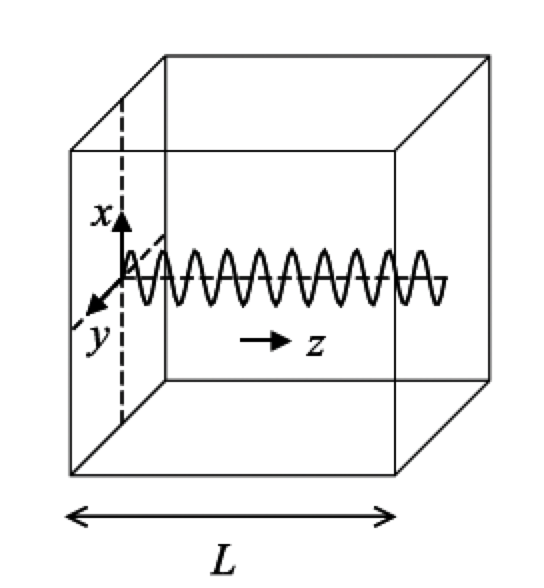
\includegraphics[width=0.45\textwidth]{figs/2022-04-27-12-37-33.png}
    \end{center}     
\end{frame}

\begin{frame}
      \frametitle{}
    经典解:
      \begin{enumerate}
        \IItem 电场:$\displaystyle E_{x}(z,t) = \sum\limits_{l=1}^{\infty } E_{0}  \sin \omega_l t \sin k_l z= \sum\limits_{l=1}^{\infty } a_l q_l (t) \sin (k_l z)$
        \IItem 磁场: $\displaystyle H_{y}(z,t) = \sum\limits_{l=1}^{\infty } H_{0}  \cos \omega_l t \cos k_l z = \sum\limits_{l=1}^{\infty } a_l \frac{\varepsilon_0}{k_l}q_l ' (t) \cos (k_l z)$  
    \end{enumerate}	  
    电磁场的能量密度: 
    \[ \omega = \frac{1}{2} (\varepsilon_0 E^2 _x + \mu_0 H^2 _y) \]
    经典哈密顿:
    \[ H = \frac{1}{2} \int_V (\varepsilon_0 E^2 _x + \mu_0 H^2 _y) dV \] 
\end{frame}

\begin{frame}
      \frametitle{}
    代入电磁场经典解, 利用腔模正交性, 得:
    \[ \begin{aligned}
        H &= \frac{1}{2} \int_V (\mu_0 \mathbf{H}^2 + \varepsilon_0 \mathbf{E}^2) dV \\ 
        &= \sum_l  \frac{1}{2}(p_l ^2 + \omega_l ^2 q_l ^2 ) \\ 
        &= \sum_l H_l  
     \end{aligned} 
    \] 
    电磁场总哈密顿是单模哈密顿的线性叠加.
\end{frame}

\begin{frame}
      \frametitle{单模量子化}
      单模哈密顿:
      \[ H_l  =  \frac{1}{2}(p_l ^2 + \omega_l ^2 q_l ^2 ) \]
      写出密顿运动方程
    \[ \begin{aligned}
        \frac{\mathrm{d}p_l}{\mathrm{d}t} &= - \frac{\partial H_l}{\partial q_l} = - \omega ^2 _l q_l \\ 
        \frac{\mathrm{d}q_l}{\mathrm{d}t} &= \frac{\partial H_l}{\partial p_l} =p_l
        \end{aligned} 
    \] 
    说明 $ p_l $ 和$q_l$ 是一对正则量.  可进行正则量子化!
\end{frame}

\begin{frame}    
    量子化条件
    \[  [\hat{q}_l,\hat{p}_l]=i\hbar \] 
    写在一起:
    \[ \hat{H}_l  =  \frac{1}{2}(\hat{p}_l ^2 + \omega_l ^2 \hat{q}_l ^2 )  \qquad \text{with} \quad [\hat{q_l},\hat{p_l}] =i\hbar\] 
    代入薛定谔方程,既可求得场的波函数! \\ {\vspace*{1em}}
  \end{frame}
  
  \begin{frame} 
  \frametitle{求解单模光场}
    单模哈密顿
    \[ \hat{H}_l  =  \frac{1}{2}(\hat{p}_l ^2 + \omega_l ^2 \hat{q}_l ^2 )  \qquad \text{with} \quad [\hat{q_l},\hat{p_l}] =i\hbar\] 
    谐振子哈密顿
    \begin{equation*}
        \hat{H} = \frac{\hat{p}^2 }{2m} + \dfrac{1}{2} m \omega ^2 \hat{x}^2   \qquad \text{with} \quad [\hat{x},\hat{p}]=i\hbar 
    \end{equation*}	
    比较: 如果令谐振子质量$m =1$, 则形式完全相同.  \\ 
    单模光场可视为单位质量的谐振子. 并称$\hat{q_l},\hat{p_l}$为电场和磁场算符\\ {\vspace*{1.3em}}
    * 机械振子通过动-势能的相互转换形成振荡, 光场通过电场能和磁场能的相互转换形成振荡!
\end{frame}

\begin{frame}   
  ~{\Bullet}具体求解与谐振子相同, 令:
    \[ \hat{Q}_l = \sqrt{\frac{\omega}{\hbar}}\hat{q_l}, \qquad \hat{P}_l = \sqrt{\frac{1}{\hbar \omega}} \hat{p_l} \]
    有:
    \[  \hat{H}_l= \frac{\hbar \omega }{2} (\hat{Q}^2 _l + \hat{P}^2 _l) \qquad \text{with} \quad [\hat{Q}_l,\hat{P}_l]=i \]
    令:
    \[ \hat{a}_l= \frac{1 }{\sqrt{2}} (\hat{Q} _l+ i\hat{P}_l ), \qquad \hat{a}^\dagger _l = \frac{1 }{\sqrt{2}} (\hat{Q}_l - i\hat{P}_l ) \]
    有
    \[
        \hat{a}_l = \frac{1}{\sqrt{2\hbar \omega_l}} (\omega_l\hat{q}_l+i \hat{p}_l)  , \qquad
        \hat{a}_l ^\dagger = \frac{1}{\sqrt{2\hbar \omega_l}} (\omega_l\hat{q}_l-i \hat{p}_l)  
    \]  
    可得产生湮灭形式:
    \[  \hat{H}_l= \hbar \omega \left(\hat{a}^\dagger _l \hat{a} _l + \frac{1 }{2}\right) \qquad \text{with} \quad [\hat{a}_l,\hat{a}^\dagger _l]=1 \]
\end{frame}

\begin{frame} 
\frametitle{}
~\\
    量子谐振子中取质量 $m=1$, 即得单模光场($\omega_l$)解 \\  \vspace*{1.3em}
    能量本征值
    \[ E_n=(n+\dfrac{1}{2})\hbar \omega_l \]
    能量本征态
    \[ \rs{n} \]
    位置表象的能量本征态
    \[ \lr{x}{n} = \frac{1}{\sqrt{n!2^n}} (\frac{\alpha}{\pi})^{\frac{1}{4}} e^{- \frac{1 }{2 } \xi^2} H_n(\xi) \]
    式中
    \[ \xi = \alpha x, \qquad \alpha =\sqrt{\frac{m \omega }{\hbar}} = \sqrt{\frac{\omega }{\hbar}}  \]
    解毕!
\end{frame}


\begin{frame}
  \frametitle{电磁场的其他物理量}
  ~\\
  根据
  \[
    \hat{a}_l = \frac{1}{\sqrt{2\hbar \omega_l}} (\omega_l\hat{q}_l+i \hat{p}_l)  , \qquad
    \hat{a}_l ^\dagger = \frac{1}{\sqrt{2\hbar \omega_l}} (\omega_l\hat{q}_l-i \hat{p}_l)  
    \]  
  反向求得: 
  \[ \begin{aligned}
     \hat{q}_l &= \sqrt{\frac{\hbar}{ 2\omega_l}} (\hat{a}_l+ \hat{a}_l ^\dagger) \\ 
     \hat{p}_l &= -i\sqrt{\frac{\hbar\omega_l}{2 }} (\hat{a}_l- \hat{a}_l ^\dagger)  
  \end{aligned} \] 
若光场的某物理量F的经典表示为:$F(q_l, p_l)$, 则其量子力学算符为: $F(\hat{q}_l, \hat{p}_l)$, 其产生湮灭算符形式也可求得. \\ {\vspace*{1.3em}}

即: 电磁场的所有经典物理量都可经由产生湮灭算求得!     
\end{frame}

\begin{frame}
    \frametitle{}
    \例 [1.求单模腔场电磁场分量的算符形式] {}
    \解 ~经典单模腔场解: 
    \[ \begin{aligned}
      E_{l}(z,t) &= a_l q_l (t) \sin (k_l z)\\
      H_{l}(z,t) &= b_l p_l (t) \cos (k_l z)
    \end{aligned}\] 
    算符:
    \[ \begin{aligned}
      \hat{E}_{x,l}(z,t) &= a_l \hat{q}_l (t) \sin (k_l z)\\
      \hat{H}_{y,l}(z,t) &= b_l \hat{p}_l (t) \cos (k_l z)
    \end{aligned}\] 
    代入
      \[ \begin{aligned}
        \hat{q}_l = \sqrt{\frac{\hbar}{ 2\omega_l}} (\hat{a}_l+ \hat{a}_l ^\dagger) , \qquad  
        \hat{p}_l = -i\sqrt{\frac{\hbar\omega_l}{2 }} (\hat{a}_l- \hat{a}_l ^\dagger)  
     \end{aligned} \] 
\end{frame}

\begin{frame} 
\frametitle{}
    产生湮灭算符描述的电场算符
    \[ 
      \hat{\mathbf{E}}_{x,l}( z,t) = E^0 _l \left(\hat{a}_l(t)+ \hat{a}_l ^\dagger(t) \right) \sin (k_l z)
      \] 
    式中 \[ E^0 _l = \sqrt{\frac{\hbar \omega_l }{\varepsilon_0 V}}\]
    三维形式
    \[ \hat{\mathbf{E}}_l(\mathbf{r},t) = E^0 _l \left(\hat{a}_l(t)+ \hat{a}_l ^\dagger(t) \right) \mathbf{E}_l(\mathbf{r}) \]
\end{frame}

\begin{frame}
  \frametitle{}
  \例 [2.试证明电场算符与占据数算符不对易] {\[ [\hat{n}, \hat{E}_x] = E_0 \sin{kz}(\hat{a}^{\dagger}-\hat{a})\]}
  \解 ~考虑单模场:
  \[ \begin{aligned}
    [\hat{n}, \hat{E}_x] &= \left[\hat{a}^{\dagger}_l \hat{a}_l, E^0 _l \left(\hat{a}_l+ \hat{a}_l ^\dagger \right) \sin (k_l z)\right] \\
    &= E^0 _l\sin (k_l z)\left[\hat{a}^{\dagger}_l \hat{a}_l,  \left(\hat{a}_l+ \hat{a}_l ^\dagger \right)\right]\\ 
    &= E^0 _l\sin (k_l z)\hat{a}^{\dagger}_l\left[ \hat{a}_l,  \left(\hat{a}_l+ \hat{a}_l ^\dagger \right)\right] + E^0 _l\sin (k_l z)\left[\hat{a}^{\dagger}_l ,  \left(\hat{a}_l+ \hat{a}_l ^\dagger \right)\right]\hat{a}_l\\
    &=  E^0 _l\sin (k_l z)\hat{a}^{\dagger}_l- E^0 _l\sin (k_l z)\hat{a}_l \\ 
    &= E_0 \sin{kz}(\hat{a}^{\dagger}-\hat{a})
  \end{aligned}\] 
  证毕!\\
  说明:电场越确定, 则光场的光子数越不确定,也即场强与相位不能同时确定。
\end{frame}

\section{2. 单模光场的量子涨落}

\begin{frame}
      \frametitle{}
    \例[3.试证明$Fock$ 态下电磁场的电场强度平均值为零]{}
    \证~
    设电磁场处于$Fock$ 态 $\rs{n}$, 取三维腔模进行计算
    \[ 
      \begin{aligned}
        \lcr{n}{\mathbf{E}(\mathbf{r,t})}{n} &= \lcr{n}{E^0  (\hat{a}+ \hat{a} ^\dagger)\mathbf{E}(\mathbf{r})}{n}   \\ 
        &= E^0 \mathbf{E}( \mathbf{r})\lcr{n}{\hat{a} }{n} + E^0 \mathbf{E}( \mathbf{r})\lcr{n}{\hat{a}^\dagger }{n}  \\ 
        &= 0+0 \\ 
        &=0 
      \end{aligned}
      \]   
      ~\\
      * 相位随机性导致测量平均值为零!  (证明见后)\\
      Fock态表象一般用于处理小粒子数的情况.  \\      
\end{frame}

\begin{frame}
    \frametitle{}
    \例[4.考虑一维单模驻波场, 求电场和磁场强度的量子涨落]{}
    \解~一维单模驻波场的电场和磁场算符为  
    \[ \begin{aligned}
      E_x(z,t)
      &= E_0  (a(t)+a^\dagger(t) )\sin (kz) \\
   \end{aligned} \]
   设光场处于$Fock$态$\rs{n}$, 有:
   \[ \lcr{n}{E_x(z,t)}{n} = \lcr{n}{H_y(z,t)}{n} =0\]
  \end{frame}

  \begin{frame}
   \[ \begin{aligned}
     \lcr{n}{E^2_x}{n} &= \lcr{n}{E^2_0 \sin^2 (kz) (a^\dagger(t)-a(t))^2}{n} \\
     &= E^2_0 \sin^2 (kz) \lcr{n}{2a^\dagger a+1}{n} \\ 
     &= 2 E^2_0 \sin^2 (kz) \lcr{n}{n+\frac{1}{2}}{n} \\ 
     &= 2 (n+\frac{1}{2})E^2_0 \sin^2 (kz)  
  \end{aligned} \]
  量子涨落: 
  \[
 \begin{aligned}
        \Delta E_x &= \sqrt{\langle E^2_x\rangle - \langle E_x\rangle ^2} \\
        &= \sqrt{2} \sqrt{n+\frac{1}{2}} E_0 \left|\sin kz \right| 
 \end{aligned} \]
 即使没有激发(n=0),依然存在真空涨落$ E_0 \left|\sin kz \right|  $  
\end{frame}

%%%%%%%%%%%%%%%%%%%%%%%%%%%%%%%%%%%%%%%%%%%%%%%%%%%%%%%%%%%%%%%%%%%
\begin{frame}
  \frametitle{课堂作业}
   \begin{block}{试证明如下重要结论}
   \[
  \begin{aligned}
   \lcr{n}{\hat{a} ^\dagger\hat{a} ^\dagger}{n} & = 0   \\     
   \lcr{n}{\hat{a} \hat{a} }{n} & =0   \\  
   \lcr{n}{\hat{a} ^\dagger\hat{a} }{n} & = n   \\   
   \lcr{n}{\hat{a} \hat{a} ^\dagger}{n} & = n+1   \\    
  \end{aligned}
  \]
   \end{block}
\end{frame}
%%%%%%%%%%%%%%%%%%%%%%%%%%%%%%%%%%%%%%%%%%%%%%%%%%%%%%%%%%%%%%%%%%%

\section{3. 光场随时间的演化}

\begin{frame}
 \frametitle{}
 {\Bullet}海森堡方程描述算符随时间的演化规律:
 \[ i\hbar\frac{\mathrm{d}F}{\mathrm{d}t} = [F,H] \]
 把$F= a $ 和光场哈密顿代入上式
 \[ \begin{aligned}
   \frac{\mathrm{d}a}{\mathrm{d}t} & =  \frac{1}{i \hbar} \left[a, \hbar \omega \left(\hat{a}^\dagger \hat{a} + \frac{1 }{2}\right)\right] \\
   &= i \omega (a^{\dagger} a a - a a^{\dagger}a)\\
   &= i \omega [a , a^{\dagger}] a \\ 
   &= - i \omega a
 \end{aligned}\] 
解得:
 \[ a(t)=a(0) e^{-i \omega t} = a e^{-i \omega t} \]  
同理,  
 \[ a ^\dagger(t)=a ^\dagger(0) e^{i \omega t} = a ^\dagger e^{i \omega t}\]  
\end{frame}

\begin{frame}
 \frametitle{}
 场算符随时间的演化:
\[ q_{l}(t)=\sqrt{\frac{\hbar}{2 \omega_{l}}}\left(a_{l} e^{-i \omega_{l} t}+a_{l}^{\dagger} e^{i \omega_{l} t}\right) \]
\[ p_{l}(t)=- i\sqrt{\frac{ \hbar \omega_{l}}{2}}\left(a_{l} e^{-i \omega_{l} t}-a_{l}^{\dagger} e^{i \omega_{l} t}\right) \]   
\end{frame}

\begin{frame}
 \frametitle{}
  场强随时间的演化 
  \[ 
    \begin{aligned}
      &E_{x}(z, t)=\sum_{l} \mathcal{E}_{l}^{(s)}\left(a_{l} e^{-i \omega t}+a_{l}^{\dagger} e^{i \omega t}\right) \sin \left(k_{l} z\right)  \\ 
      &B_{y}(z, t)=-i \sum_{l} \mathcal{B}_{l}^{(s)}\left(a_{l} e^{-i \omega t}-a_{l}^{\dagger} e^{i \omega t}\right) \cos \left(k_{l} z\right)  \\   
    \end{aligned} 
  \]
式中 $\mathcal{E}_{l}^{(s)}=\sqrt{\frac{\hbar \omega_{l}}{\varepsilon_{0} V}}, \quad
\mathcal{B}_{l}^{(s)}=\frac{\mu_0}{k_l}\sqrt{\frac{\varepsilon_{0}\hbar \omega_{l} ^3}{V}}$
\end{frame}

\section{4. 量子化相图}

\begin{frame}
  \frametitle{经典相图}
  考虑空腔中的一个线性极化的电磁波,如图
    \begin{center}
       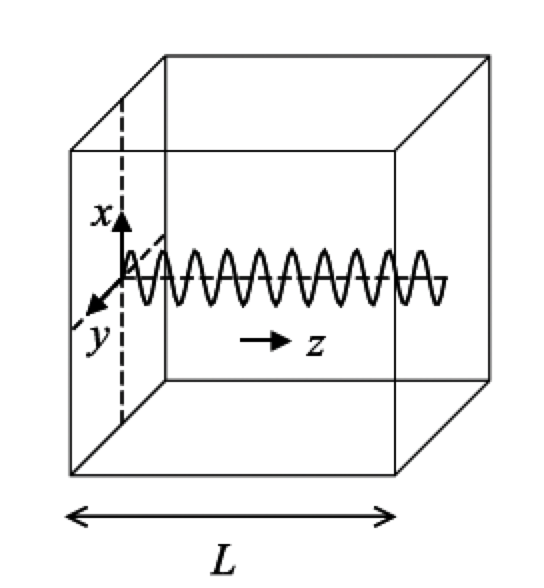
\includegraphics[width=0.24\textwidth]{figs/2022-04-27-12-37-33.png}
    \end{center}
   场分量如下:  
   \[ \begin{cases}
    E_{x}(z, t)=E_{0} \sin \omega t\sin k z  \\ 
    B_{y}(z, t)=B_{0} \cos \omega t \cos k z,  \quad \text{with} \quad B_{0} = E_{0} /c 
   \end{cases} \]
 \end{frame}
 
%\begin{frame}
% \frametitle{}
% 电磁场的能量密度为:
% \[ H=\frac{1}{2}\left(\epsilon_{0} {E}^{2}+\frac{1}{\mu_{0}} B^{2}\right) \]
% 电场能 (设模面积为A): 
% \[ \begin{aligned}
%  E_{\text {electric }} &=\frac{1}{2} \epsilon_{0} A \int_{0}^{L} {E}_{0}^{2} \sin ^{2} k z \sin ^{2} \omega t \mathrm{~d} z \\
%  &=\frac{1}{4} \epsilon_{0} A {E}_{0}^{2} \sin ^{2} \omega t \int_{0}^{L}(1-\cos 2 k z) \mathrm{d} z \\
%  &=\frac{1}{4} \epsilon_{0} V {E}_{0}^{2} \sin ^{2} \omega t
%  \end{aligned}
%    \]       
%\end{frame}
%
%\begin{frame}
% \frametitle{}
% 磁场能 :  
% \[\begin{aligned}
%  E_{\text {magnetic }} &=\frac{1}{2 \mu_{0}} A \int_{0}^{L} B_{0}^{2} \cos ^{2} k z \cos ^{2} \omega t \mathrm{~d} z \\
%  &=\frac{1}{4 \mu_{0}} A B_{0}^{2} \cos ^{2} \omega t \int_{0}^{L}(1+\cos 2 k z) \mathrm{d} z \\
%  &=\frac{1}{4 \mu_{0}} V B_{0}^{2} \cos ^{2} \omega t
%  \end{aligned} \] 
%总能量 :
%\[ H=\frac{V}{4}\left(\epsilon_{0} \mathcal{E}_{0}^{2} \sin ^{2} \omega t+\frac{B_{0}^{2}}{\mu_{0}} \cos ^{2} \omega t\right)
%   \]
%\end{frame}
%
%begin{frame}
% \frametitle{}
% 令: \[ q(t)=\left(\frac{\epsilon_{0} V}{2 \omega^{2}}\right)^{1 / 2} \mathcal{E}_{0} \sin \omega t \]
% \[ p(t)=\left(\frac{V}{2 \mu_{0}}\right)^{1 / 2} B_{0} \cos \omega t \equiv\left(\frac{\epsilon_{0} V}{2}\right)^{1 / 2} \mathcal{E}_{0} \cos \omega t \]
% 代回, 得总能:
%     \[ H=\frac{1}{2}\left(p^{2}+\omega^{2} q^{2}\right) \]
% 说明电磁场的振荡是电场能与磁场能之间的转换
%end{frame}

\begin{frame}
 \frametitle{}
 初始条件决定一个初始相位 $ \varphi$ \\ 
  {\Bullet}复函表示:  \[
    \begin{aligned}
         E_{x}(z, t) &= E_{0} \sin (\omega t+\varphi) \sin k z \\
         &=E_{0} (z,t) e^ {i\varphi}  \\
         &=  E_{0}(z,t) \cos\varphi  + i E_{0}(z,t) \sin\varphi \\ 
         &= E_1 (z,t) + i E_2 (z,t)
    \end{aligned}
    \]
  其中 $E_1(z,t), E_2(z,t) $是电场的实部和虚部 \\   
\end{frame}

\begin{frame}
   \begin{center}
      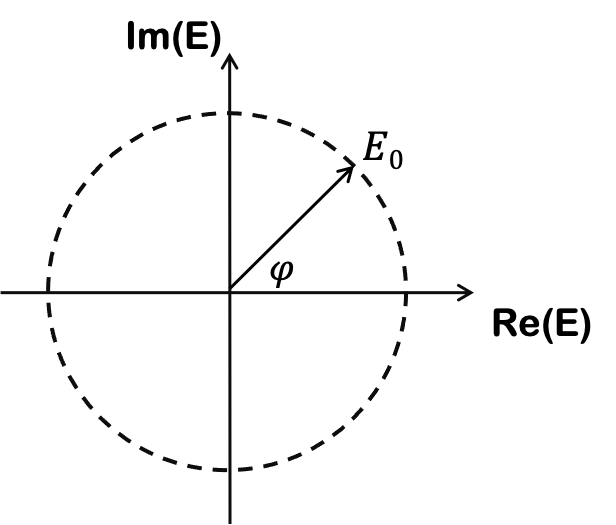
\includegraphics[width=0.4\textwidth]{figs/2.png}
   \end{center}
 \[ \begin{cases}
  Re(E)= E_{0}(z,t) \cos\varphi\\ 
  Im(E)= E_{0}(z,t) \sin\varphi\\ 
 \end{cases} \]
 电磁场的大小和相位角都是确定的.  
\end{frame}

\begin{frame}
  \frametitle{}
  定义电场的正交分量(field quadratures)
  \[ \begin{cases}
    X_{1}(t) = \sqrt{\frac{\omega}{2\hbar}}q(t)= \sqrt{\frac{\varepsilon_{0} V}{4 \hbar \omega}} {E}_{0} \sin \omega t\\ 
    X_{2}(t) = \sqrt{\frac{1}{2\hbar \omega}}p(t)= \sqrt{\frac{\varepsilon_{0} V}{4 \hbar \omega}} {E}_{0} \cos \omega t\\ 
   \end{cases} \]
   代入
   \[
  \begin{aligned}
       E_{x}(z, t) &=E_{0} \sin k z \sin (\omega t + \varphi) \\
       &=  E_{0} \sin k z (\cos\varphi \sin\omega t + \sin\varphi \cos\omega t) \\ 
       &= \sqrt{\frac{4 \hbar \omega}{\varepsilon_{0} V}} \sin k z\left(\cos \varphi X_{1}(t)+\sin \varphi X_{2}(t)\right) \\ 
       &=  X_{1}(z,t)+ i X_{2}(z,t)
  \end{aligned}
  \]
\end{frame}

\begin{frame}
  \begin{center}
     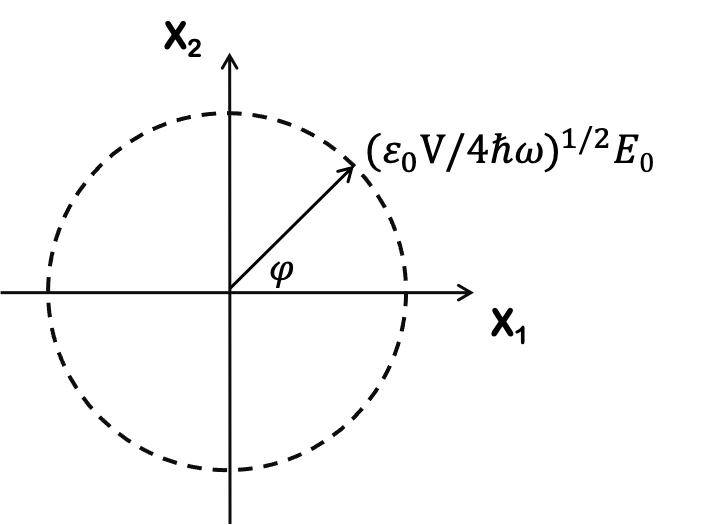
\includegraphics[width=0.5\textwidth]{figs/3.png}
  \end{center}
\end{frame}


\begin{frame}
  \frametitle{量子化相图}
  场正交分量可量子化:
  \[ \begin{cases}
    \hat{X}_{1}(t) = \sqrt{\frac{\omega_l}{2\hbar}}\hat{q}(t)=\frac{1}{2}\left(a+a^{^{\dagger}}\right)\\ 
    \hat{X}_{2}(t) = \sqrt{\frac{1}{2\hbar \omega_l}}\hat{p}(t)= \frac{1}{2 i}\left(a-a^{^{\dagger}}\right)\\ 
   \end{cases} \]
  \[ \text{with} \, [X_1, X_2] =\frac{i}{2} \]
  计算不确定度:
  \[ \Delta X_1 \Delta X_2  = \frac{1}{2\hbar}  \Delta q \Delta p \geq \frac{1}{2\hbar} \frac{\hbar}{2}=\frac{1}{4}  \]
\end{frame}

\begin{frame}
    \frametitle{} 
    \begin{center}
       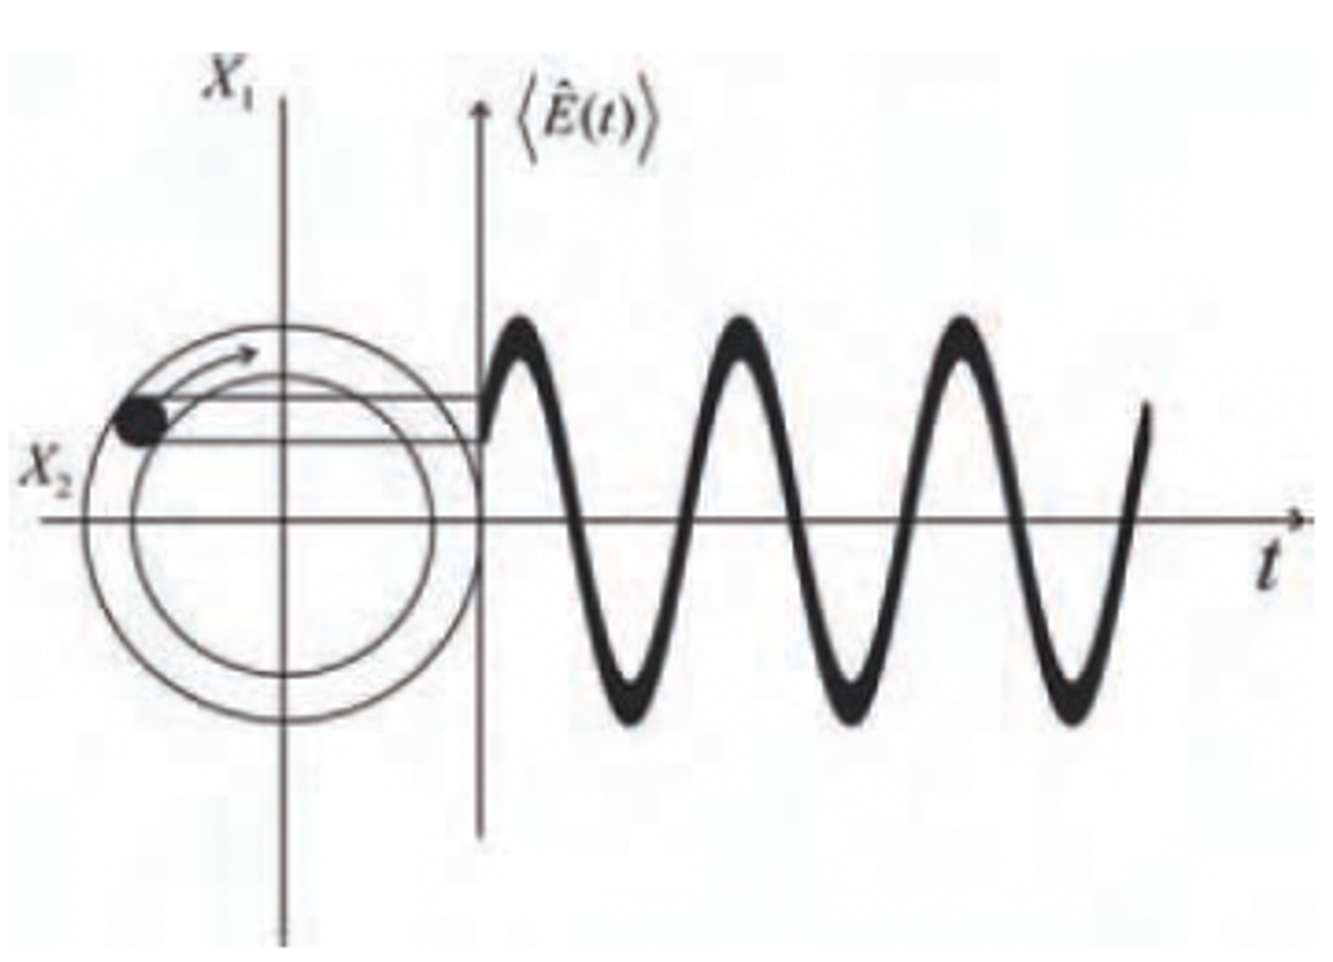
\includegraphics[width=0.55\textwidth]{figs/34.png}
    \end{center}
    \[ \Delta X_1 \Delta X_2  \geq  \frac{1}{4}  \]
    电磁场的大小和相位角都有一定的不确定性. 黑色区描述不可区分的简并态. 
\end{frame}

\begin{frame}
  \frametitle{}
  \例[5.试证明真空态是最小不确定度乘积态]{
   \[ \Delta X_1 \Delta X_2 =\dfrac{1}{4} \] 
  }
  \解~不确定度计算公式\[ \Delta x  = \sqrt{ \overline{x^2}- \overline{x}^2}\] 
\[ 
\begin{aligned}
  \overline{ X_1}  &= \lcr{n}{\frac{1}{2}\left(a+a^{\dagger}\right)}{n} \\ 
        &= 0 \\
  \overline{ X_2 } &= \lcr{n}{\frac{1}{2i}\left(a-a^{\dagger}\right)}{n} \\ 
        &= 0 
\end{aligned}\]
\end{frame}

\begin{frame}
  \frametitle{}
\[ 
\begin{aligned}
  \overline{X_1 ^2} &= \lcr{n}{\frac{1}{4}\left(a+a^{\dagger}\right)^2}{n} \\
        &= \frac{1}{4} \lcr{n}{\left(aa+a^{\dagger}a^{\dagger}+aa^{\dagger}+ a^{\dagger}a\right)}{n} \\
        &= \frac{1}{4} (2n+1)
\end{aligned}\]
\[
\begin{aligned}
  \overline{X_2 ^2} &= \lcr{n}{-\frac{1}{4}\left(a-a^{\dagger}\right)^2}{n} \\
  &= -\frac{1}{4} \lcr{n}{\left(aa+a^{\dagger}a^{\dagger}-aa^{\dagger}- a^{\dagger}a\right)}{n} \\
  &= \frac{1}{4} (2n+1)
\end{aligned}\]
\[ \Delta X_1 = \Delta X_2  =  \sqrt{ \overline{X^2}- \overline{X}^2} =\frac{1}{2}\sqrt{2n+1}\geq \frac{1}{2}\] 
\end{frame}

\begin{frame}
 \frametitle{}
  对于真空态
 \[ \Delta X_1 = \Delta X_2  = \frac{1}{2}\]
 即:
 \[ \Delta X_1 \Delta X_2  = \frac{1}{4}\]    
 证毕!\\ 
\end{frame}

\begin{frame}
 \frametitle{真空态相图}
真空态的经典电场能$E_0=0$, 电场矢量大小为零, 处于原点. 是相位完全不确定的态. 
      \begin{center}
         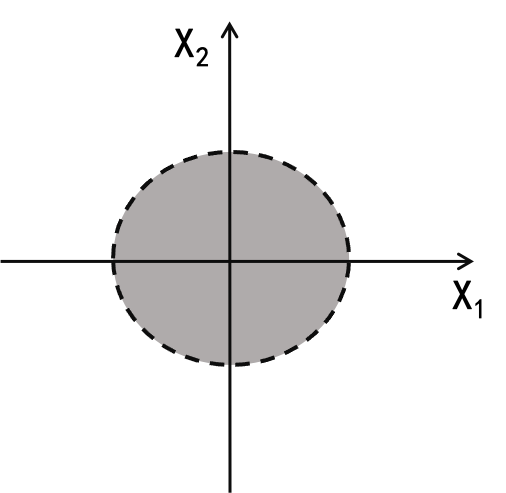
\includegraphics[width=0.28\textwidth]{figs/4.png}
      \end{center}
      \[ \Delta X_1 = \Delta X_2  = \frac{1}{2}\]
真空态的量子涨落为量子噪音的极限(极小值$\dfrac{1}{4}$) 
\end{frame}

\section{5. 相位算符}

\begin{frame} 
  \frametitle{相位算符的定义}
       经典光场的复振幅 
       \[ a= \left|a\right| e^{i\varphi}\]
       经典光场的正则分量
       \[ q(t) = a e^{-\omega t} + a e^{\omega t} = 2\left|a \right|\cos(\omega t + \varphi)\]
       (1) 那是否可写出一个相位算符呢?, 比如把湮灭算符写成
       \[ \hat{a} = \hat{g} e ^ {i \hat{\varphi}} \]
       这种写法是不行的, 因为
       $e ^ {i \hat{\varphi}}$与$e ^ {-i \hat{\varphi}}$ 并不是幺正的, 会导致 $\hat{\varphi}$不是厄密的,因而没有可测量意义. 
\end{frame}

\begin{frame} 
    \frametitle{}
    ~\\
       (2) 为保证厄密, Susskind–Glogower, 令
       \[ \rs{\varphi} = \sum_ {n=0} ^ \infty e^{i (n\varphi)} \rs{n} \]
       定义指数算符
       \[ \hat {e} \rs{\varphi}= e^{i {\varphi}}\rs{\varphi} \] 
        \[ \ls{\varphi}  e^{-i {\varphi}} = \ls{\varphi} \hat{e}^{\dagger}\]
      可得指数算符与产生湮灭算符的关系
      \[ \hat {e} = \frac{1}{\sqrt{\hat{n}+1}} \hat {a} =  \frac{1}{\sqrt{\hat {a}\hat {a}^{\dagger}}} \hat {a} \] 
      \[ \hat {e}^{\dagger} = \hat {a}^{\dagger} \frac{1}{\sqrt{\hat{n}+1}} = \hat {a}^{\dagger} \frac{1}{\sqrt{\hat {a}\hat {a}^{\dagger}}}  \] 
\end{frame}

\begin{frame} 
\frametitle{}
定义新的相位算符
\[\hat{C}= \frac{1}{2} (\hat {e} + \hat {e}^{\dagger})=\frac{1}{2}\left[ \frac{1}{\sqrt{\hat{n}+1}}a + a^{\dagger}  \frac{1}{\sqrt{\hat{n}+1}}\right]\]
\[\hat{S}= \frac{1}{2i} (\hat {e} - \hat {e}^{\dagger})=\frac{1}{2i}\left[ \frac{1}{\sqrt{\hat{n}+1}}a - a^{\dagger}  \frac{1}{\sqrt{\hat{n}+1}}\right]\]
       反向求得 
       \[\hat{a}= \sqrt{\hat{n}+1}(\hat{C}+i\hat{S})\]
       \[\hat{a}^{\dagger}= (\hat{C}-i\hat{S})\sqrt{\hat{n}+1}\]
\end{frame}

\begin{frame} 
\frametitle{}
    \例 [6. 试证明指数算符有如下性质]
    {\[ \hat {e} \rs{n} = \rs{n-1}, \qquad \hat {e}^{\dagger} \rs{n} = \rs{n+1}\]}
    \证 ~
    \[ \begin{aligned}
      \hat {e} \rs{n} & = \frac{1}{\sqrt{\hat{n}+1}} \hat {a} \rs{n}\\
      &= \frac{1}{\sqrt{\hat{n}+1}}  \sqrt{n} \rs{n-1} \\
      &= \frac{1}{\sqrt{(n-1)+1}}  \sqrt{n} \rs{n-1}  \\ 
      &= \rs{n-1}
    \end{aligned}\] 
\end{frame}

\begin{frame} 
\frametitle{相位算符的性质}
性质(1):
\[ \begin{aligned}
        S \rs{n} &= \frac{1}{2i} [\rs{n-1}+\rs{n-1}]\\
        S \rs{0} &=-\frac{1}{2i} \rs{1}\\
        S^2 \rs{n}&= \frac{1}{4} [\rs{n}+\rs{n}- \rs{n-2}-\rs{n+2}] \\  
     \end{aligned}\] 
\end{frame}

%\begin{frame} 
%\frametitle{}
%相干态的相位均值:
%    \[  \left\langle \alpha |C| \alpha   \right\rangle = %\left|\alpha\right|\cos\theta \exp(-\left|\alpha\right|%^2) \sum_n \frac{\left|\alpha\right|^{2n}}{n! \sqrt{n+1}%} \]
%    当 $\left|\alpha\right|^2\gg 1$时
%    \[  \left\langle \alpha |\cos \varphi| \alpha   %\right\rangle = \cos \theta (1+ \frac{1}{8\left|%\alpha\right|^2}+ \cdots )\]
%    \[  \left\langle \alpha |\sin \varphi| \alpha   %\right\rangle = \cos^2 \theta -\frac{\cos^2 \theta %-\frac{1}{2}}{2\left|\alpha\right|^2 } \]   
%\end{frame}

\begin{frame} 
\frametitle{}
性质(2):
\[ \begin{aligned}
        [C, S] & = \frac{1}{2}i \rl{0}{0}\\
        [C, \hat {n} ] & = i S \\ 
        [S, \hat {n} ] & = -i C \\ 
        C^2 + S^2 &= 1-\frac{1}{2} \rl{0}{0} 
     \end{aligned}\] 
(3) 数态的相位均值
   \[ \left\langle n|C|n \right\rangle = \left\langle n|S|n \right\rangle =0 \]
这正是光场电磁分量均值为零的原因
   \[ \left\langle n|C^2|n \right\rangle = \left\langle n|S^2|n \right\rangle = 
   \begin{cases}
    \frac{1}{2} \quad  n \ge 1 \\ 
    ~\\
    \frac{1}{4} \quad  n = 0
   \end{cases} \]
\end{frame}

\begin{frame} 
\frametitle{}
    \例 [7. 设光场处于数态叠加态, 求相位分布函数]{}
    \解 ~光场 
    \[ \rs{\psi} = \sum c_n \rs{n} \]
     方法(1) : \\
    相位表象的波函数
     \[ \lr{\varphi}{\psi} = \sum_ {n=0} ^ \infty e^{-i (n\varphi)} c_n \lr{n} {n} \]
     相位分布 
     \[ \begin{aligned}
       P(\varphi) &= \frac{1}{2 \pi} |\lr{\varphi}{\psi} |^2 \\
       &= \frac{1}{2 \pi} | \sum_ {n=0} ^ \infty e^{-i (n\varphi)} c_n  |^2 \\
     \end{aligned}\] 
     对于具体的叠加态, 可得分布函数
\end{frame}

\begin{frame} 
\frametitle{}
     方法(2) : \\
     密度算符
     \[ \rho = \rl{\psi}{\psi} \]
     相位分布
     \[ \begin{aligned}
      P(\varphi) &= \frac{1}{2 \pi} \lcr{\varphi}{\rho} {\varphi} \\
      &= \frac{1}{2 \pi} \lr{\varphi}{\psi} \lr{\psi}{\varphi} \\
      &= \cdots
    \end{aligned}\] 
     * 密度算符方法算混态更方便...
     \[ \rho = \sum_j P_j\rl{\psi_j}{\psi_j} \]
\end{frame}

\section{6. 自由光场的量子化}

\begin{frame}
      \frametitle{自由光场的单模量子化}
      自由空间电磁场为平面波(行波解):
      \[  \hat{e}_\sigma exp (\pm i (\omega_k t - \mathbf{k}\cdot \mathbf{r})), \qquad k^2 =\frac{\omega_k ^2}{c^2} \]
      式中 $\hat{e}_\sigma $ 为偏振方向上的单位矢量, $\sigma=\pm$ 代表两个振动方向, 它们相互正交且都与波矢$\mathbf{k}$正交. \\ \vspace*{1em} 
      经箱归一化, 可离散化行波, 得 
      \[ \mathbf{k} = \frac{2\pi}{L} (l_1 \mathbf{i} + l_2 \mathbf{j}+ l_3 \mathbf{k}), \qquad l_i= 0, \pm 1, \pm 2, \cdots \]
      行波本征模为
      \[ \mathbf{u}_{k\sigma} (\mathbf{r}) = \hat{e}_\sigma e^{i \mathbf{k}\cdot \mathbf{r}}\]
\end{frame} 

\begin{frame}
      \frametitle{}
    自由空间电磁场行波展开
      \[   \begin{aligned}
        \mathbf{E} (\mathbf{r},t) &=i \sum^\infty _{k,\sigma} (\frac{\hbar\omega_k}{2 \epsilon_0 V } )^{1/2} \hat{e}_\sigma [ a_{k\sigma} (t) e^{i \mathbf{k}\cdot \mathbf{r}} - a ^* _{k\sigma} (t)  e^{-i \mathbf{k}\cdot \mathbf{r}}] \\
      \mathbf{H} (\mathbf{r},t) &=i \sum^\infty _{k,\sigma} (\frac{\hbar\omega_k}{2 \mu_0 V } )^{1/2} (\hat{e}_k \times \hat{e}_\sigma) [ a_{k\sigma} (t) e^{i \mathbf{k}\cdot \mathbf{r}} - a ^* _{k\sigma} (t)  e^{-i \mathbf{k}\cdot \mathbf{r}}] 
      \end{aligned} \]
    箱内总能量:
      \[ \begin{aligned}
        H &= \frac{1}{2} \int_V (\mu_0 \mathbf{H}^2 + \epsilon_0 \mathbf{E}^2) dV \\ 
        &= \frac{1}{2}\sum^\infty _{k,\sigma} (p_{k\sigma} ^2 + \omega_k ^2 q_{k\sigma} ^2 )  \\ 
        & = \sum^\infty _{k,\sigma} H_{k\sigma}
      \end{aligned} 
      \] 
\end{frame}

\begin{frame}
      \frametitle{}
      单色行波的哈密顿
      \[ H_{k\sigma} = \frac{1}{2} (p_{k\sigma} ^2 + \omega_k ^2 q_{k\sigma} ^2)\]
      哈密顿运动方程
        \[ \begin{aligned}
        \frac{\mathrm{d}p_{k\sigma}}{\mathrm{d}t} &= - \frac{\partial H_{k\sigma}}{\partial q_{k\sigma}} = - \omega ^2 _{k\sigma} q_{k\sigma} \\ 
        \frac{\mathrm{d}q_{k\sigma}}{\mathrm{d}t} &= \frac{\partial H_{k\sigma}}{\partial p_{k\sigma}} =p_{k\sigma}
        \end{aligned} 
      \] 
\end{frame}

\begin{frame}        
      同理,正则量子化
      \[ \hat{H}_{k\sigma} = \frac{1}{2} (\hat{p}_{k\sigma} ^2 + \omega_k ^2 \hat{q}_{k\sigma} ^2) \qquad \text{with} \quad [\hat{p}_{k\sigma},\hat{q}_{k\sigma}] =i\hbar \]

      \[ \hat{H}_{k\sigma}= \hbar \omega_{k\sigma} \left(\hat{a}^\dagger _{k\sigma} \hat{a} _{k\sigma}+ \frac{1 }{2}\right) \qquad \text{with} \quad [\hat{a} _{k\sigma},\hat{a}^\dagger _{k\sigma}]=1 \]
      行波电场和磁场算符:
      \[ \begin{cases}
        \hat{\mathbf{E}} (\mathbf{r},t)&=i \sum^\infty _{k,\sigma} (\frac{\hbar\omega_k}{2 \epsilon_0 V } )^{1/2} \hat{e}_\sigma [ \hat{a} _{k\sigma} (t) e^{i \mathbf{k}\cdot \mathbf{r}} - \hat{a} ^\dagger _{k\sigma} (t)  e^{-i \mathbf{k}\cdot \mathbf{r}}] \\
        &= \hat{\mathbf{E}}^+(\mathbf{r},t)+ \hat{\mathbf{E}}^-(\mathbf{r},t) \\
        ~\\
      \hat{\mathbf{H}} (\mathbf{r},t) &=i \sum^\infty _{k,\sigma} (\frac{\hbar\omega_k}{2 \mu_0 V } )^{1/2} (\hat{e}_k \times \hat{e}_\sigma) [ \hat{a} _{k\sigma} (t) e^{i \mathbf{k}\cdot \mathbf{r}} - \hat{a} ^\dagger _{k\sigma} (t)  e^{-i \mathbf{k}\cdot \mathbf{r}}] 
      \end{cases} \]
\end{frame}

\begin{frame}
  \frametitle{}
  \例[8.考虑单模行波场, 求电场和磁场强度的量子涨落]{}
  \解~ 单模行波场的电场为
  \[ \mathbf{E}_l(\mathbf{r},t) = E_{0} (\hat{a}_l\exp^{-i \omega t + i \mathbf{k}\cdot \mathbf{r}} + \hat{a}_l ^\dagger \exp^{i \omega t - i \mathbf{k}\cdot \mathbf{r}})\]
  设光场处于$Fock$态$\rs{n}$, 电场的平均值: 
\[ 
\begin{aligned}
        \left\langle \mathbf{E}_l(\mathbf{r},t) \right\rangle &=\lcr{n}{\mathbf{E}_l(\mathbf{r},t)}{n} \\  
        &= \lcr{n}{E_{0} (\hat{a}_l \exp^{-i \omega t + i \mathbf{k}\cdot \mathbf{r}} +\hat{a}_l ^\dagger \exp^{i \omega t - i \mathbf{k}\cdot \mathbf{r}})}{n}\\ 
        &=0 
\end{aligned}\]
\end{frame}

\begin{frame}
  \frametitle{}
  \[ \begin{aligned}
    \left\langle \mathbf{E}^2_l(\mathbf{r},t) \right\rangle &=\lcr{n}{\mathbf{E}^2_l(\mathbf{r},t)}{n} \\  
    &= E^2_{0} \lcr{n}{(\hat{a}_l \exp^{-i \omega t + i \mathbf{k}\cdot \mathbf{r}} +\hat{a}_l ^\dagger \exp^{i \omega t - i \mathbf{k}\cdot \mathbf{r}})^2}{n}\\ 
    &= E^2_{0} \lcr{n}{\hat{a}_l\hat{a}_l ^\dagger + \hat{a}_l ^\dagger \hat{a}_l}{n}\\ 
    &= E^2_{0} \lcr{n}{\sqrt{(n+1)(n+1)} + \sqrt{nn}}{n}\\ 
    &= E^2_{0} (2n+1)
\end{aligned}\]
量子涨落: 
\[
\begin{aligned}
    \Delta \mathbf{E}_l &= \sqrt{\langle \mathbf{E}^2 _l \rangle - \langle \mathbf{E}_l \rangle ^2} \\
    &= E_0 \sqrt{2n+1}
\end{aligned} \]
即使没有激发(n=0),依然存在真空涨落$ E_0 $  
\end{frame}

\begin{frame} 
\frametitle{多模光场的量子化}
  能量是对所有模求和
   \[ \hat{H} = \sum_l \hbar \omega_l (\hat{n}_l + \frac{1}{2}) = \sum_l \frac{1}{2} \hbar \omega_l(a^{\dagger}_l a_l + a_la^{\dagger}_l ) \]
   能量本征态是各模数态的张量积
   \[ \rs{\{n_l\}}=\rs{n_1}\otimes \rs{n_2}\otimes \rs{n_3}\cdots\rs{n_l}\cdots = \rs{n_1, n_2, n_3, \cdots, n_l,\cdots }\]
  能量本征方程
  \[ \hat{H} \rs{\{n_l\}} = E \rs{\{n_l\}}\]
  根据张量空间运算法则
  \[ \hat{a}_l \rs{\{n_l\}} = \sqrt{n_l} \rs{n_1, n_2, n_3, \cdots, n_l-1,\cdots }\]
  \[  \ls{n_1, n_2, n_3, \cdots, n_l+1,\cdots }\sqrt{n_l+1}=  \ls{\{n_l\}}\hat{a}^{\dagger}_l \]
\end{frame}

\begin{frame} 
  \frametitle{}
  \例[9. 计算双模场算符Q的均值]{
    \[  Q= \Omega \sum_{i,j,k,l} a^{\dagger} _i a^{\dagger} _j a_k a_l, \qquad i,j,k,l =1,2 \]}
    \解 双模应对双光子态进行计算
    \[ \begin{aligned}
        \overline{Q}&= \left\langle n_1 n_2|Q|n_2n_1  \right\rangle \\
        &= \Omega[\left\langle n_1 n_2|a^{\dagger} _1 a^{\dagger} _1 a_1 a_1|n_2n_1  \right\rangle + \left\langle n_1 n_2|a^{\dagger} _1 a^{\dagger} _2 a_1 a_2|n_2n_1  \right\rangle \\ 
        & + \left\langle n_1 n_2|a^{\dagger} _1 a^{\dagger} _2 a_1 a_2|n_2n_1  \right\rangle  
        + \left\langle n_1 n_2|a^{\dagger} _2 a^{\dagger} _2 a_2 a_2|n_2n_1  \right\rangle]  \\
        &= \Omega [(n_1 ^2 -n_1) + (n_2 ^2 -n_2) +4n_1 n_2 ]
    \end{aligned}\]    
 \end{frame}

 \begin{frame} 
 \frametitle{}
     * 计算第一项 
  \[ \begin{aligned}
  \left\langle n_1 n_2|a^{\dagger} _1 a^{\dagger} _1 a_1 a_1|n_2n_1  \right\rangle  &= \left\langle n_1|a^{\dagger} _1 a^{\dagger} _1 a_1 a_1|n_1  \right\rangle \\ 
  &= \left\langle n_1|a^{\dagger} _1 (a_1a^{\dagger} _1 -1) a_1|n_1  \right\rangle \\ 
  &= \left\langle n_1|(a^{\dagger} _1 a_1a^{\dagger} a_1 - a^{\dagger} a_1) |n_1  \right\rangle \\ 
  &= \left\langle n_1|(a^{\dagger} _1 a_1)^2 |n_1 \right\rangle - \left\langle n_1| a^{\dagger} a_1 |n_1  \right\rangle\\ 
  &= \left\langle n_1|\hat{n}^2 _1 |n_1 \right\rangle - \left\langle n_1| \hat{n}_1 |n_1  \right\rangle\\ 
  &= n_1 ^2 -n_1
 \end{aligned}\]
 * 课堂作业: 计算第二项
\end{frame}

\begin{frame} 
  \frametitle{小结:}
    (1) 光场哈密顿可分解为一系列场谐振子哈密顿
    \[ \hat{H}_{k\sigma}= \sum_{k,\sigma}\hbar \omega_{k\sigma} \left(\hat{a}^\dagger _{k\sigma} \hat{a} _{k\sigma}+ \frac{1 }{2}\right) \qquad \text{with} \quad [\hat{a} _{k\sigma},\hat{a}^\dagger _{k\sigma}]=1 \]
    (2) 自由光场可表示为一系列量子化的平面波 
    \[\begin{aligned}
      \hat{\mathbf{E}} (\mathbf{r},t) &=i \sum^\infty _{k,\sigma} (\frac{\hbar\omega_k}{2 \epsilon_0 V } )^{1/2} \hat{e}_\sigma \left[ \hat{a} _{k\sigma} (t) e^{i \mathbf{k}\cdot \mathbf{r}} - \hat{a} ^\dagger _{k\sigma} (t)  e^{-i \mathbf{k}\cdot \mathbf{r}}\right] \\
      &= \hat{\mathbf{E}}^+(\mathbf{r},t)+ \hat{\mathbf{E}}^-(\mathbf{r},t)
    \end{aligned} \]
    (3) 腔场则可表示为一系列量子化的驻波
  \end{frame}

%%%%%%%%%%%%%%%%%%%%%%%%%%%%%%%%%%%%%%%%%%%%%%%%%%%%%%%%%%%%%%%%%%%
\begin{frame}
    \frametitle{课外作业}
    \begin{enumerate}
        \item  利用腔模正交性证明 \[ H= \sum_l H_l\]
        \item  计算电磁场真空态的量子涨落
        \item  试证明,只有光场处于两相临数态的叠加态时,电场算符的均值才不为零
        \item  已知光场处于如下混态, 求相位分布  \[ \rho = \frac{1}{2}(\rl{0}{0} + \rl{1}{1} ) \]
    \end{enumerate}
\end{frame}
%%%%%%%%%%%%%%%%%%%%%%%%%%%%%%%%%%%%%%%%%%%%%%%%%%%%%%%%%%%%%%%%%%%    % 光场量子化
%
%%%%%%%%%%%%%%%%%%%%%%%%%%%%%%%%%%%%%%%%%%%%%%%%%%%%%%%%%%%%%
\begin{frame} [plain]
    \frametitle{}
    \Background[1] 
    \begin{center}
    {\huge 第6-7讲:相干态}
    \end{center}  
    \addtocounter{framenumber}{-1}   
\end{frame}
%%%%%%%%%%%%%%%%%%%%%%%%%%%%%%%%%%%%%%%%%%%%%%%%%%%%%%%%%%%% 

\section{1. 相干态的定义}

\begin{frame}
 \frametitle{相干态的定义}
 相干态: 也叫做格劳伯态, 是罗伊·格劳伯于1963年提出来的一种量子力学纯态, 它是数态的相干叠加态. (2005年诺贝尔物理学奖)。
 \[ \rs{\alpha} = \sum_{n=0} ^{+\infty} c_n  \rs{n} = e^{-\frac{1}{2}\left|\alpha\right|^2}  \sum_{n=0} ^{+\infty}  \frac{\alpha^n}{\sqrt{n!}} \rs{n} \]
   \begin{center}
        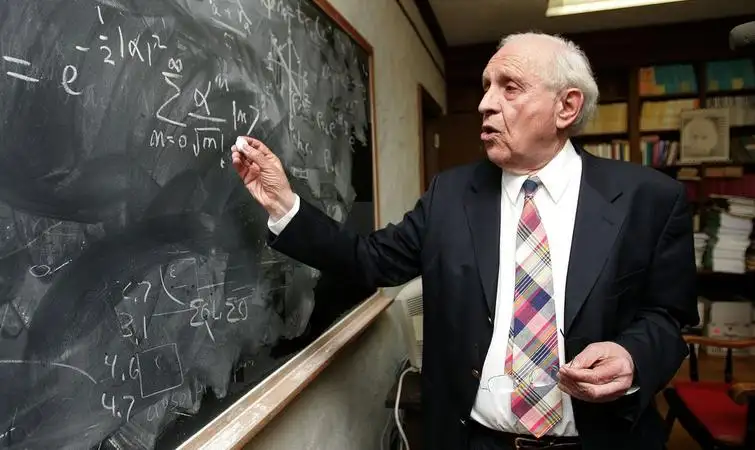
\includegraphics[width=0.5\textwidth]{figs/2022-04-27-11-50-32.png}
   \end{center}
\end{frame}

%\begin{frame}
% \frametitle{相干的经典经验}
%    经典相干三条件: 频率相同, 相差恒定, 传播方向相同.
% \begin{itemize}
%     \item 电谐振动的振动模式的空间传播形成电磁波
%     \item 频率相同的波是相干波
%     \item 谐振子拉离平衡位置(平移), 然后舒放 (起振)
%     \item 起振后谐振子的频率与拉离的距离无关 (固有频率)
%     \item 谐振子的能量与拉离的距离有关
% \end{itemize}
%    经验: 平移(拉离平衡位置) 产生相干态!    
%\end{frame}


\begin{frame} 
    \begin{tcolorbox4}[相干态基本命题:]
        \begin{enumerate}
            \item 湮灭算符的本征态是光场相干态
            \[ \hat{a}\rs{\alpha}= \alpha\rs{\alpha}\]
            \item 光场相干态源于真空态的平移
            \[ \hat{a} =  D(\alpha)  \rs{0}  \]
            \item 光场相干态具有超完备性
            \[ \frac{1}{\pi} \int \rl{\alpha}{\alpha}d ^2 \alpha =1\]
        \end{enumerate}  
    \end{tcolorbox4}
\end{frame}


\section{2. 湮灭算符的本征态}

\begin{frame}
    \frametitle{湮灭算符的本征态}
    设湮灭算符有属于本征值$\alpha$的本征态 $\rs{\alpha}$, 写本征方程: 
    \[ \hat{a}\rs{\alpha}= \alpha\rs{\alpha}\]
    \[ \ls{\alpha}\alpha^* =\ls{\alpha}\hat{a}^\dagger\]
    * 相干态是湮灭一个光子后,场的状态没有发生改变的态 (如何理解?)\\  {\vspace*{0.6em}}
    湮灭算符不厄密, 本征值不是实数, 对应经典的复振幅. 
    \[ \alpha =\left|\alpha\right| e^{i\varphi} = X_1 + i X_2\]
    \[ \alpha^* =\left|\alpha\right| e^{-i\varphi} = X_1 - i X_2\]
\end{frame}

\begin{frame}
    \frametitle{}     
    \例 [1. 试在$Fock$表象求湮灭算符的本征态]{}
    \解 ~对于本征方程
    \[ a \rs{\alpha} = \alpha \rs{\alpha} \]
    把本征态在$Fock$表象展开 
  \[\begin{aligned}
      a \rs{\alpha} &=\sum_{n=0} ^{+\infty} c_n a \rs{n} \\
      &=  \sum_{n=1} ^{+\infty} c_n \sqrt{n} \rs{n-1} \\
      &=  \sum_{n=0} ^{+\infty} c_{n+1} \sqrt{n+1} \rs{n} \\
      &=   \alpha \sum_{n=0} ^{+\infty} c_n  \rs{n}  
  \end{aligned} \]
\end{frame}

\begin{frame}
    \frametitle{}
    得递推公式
    \[\begin{aligned}
      c_{n+1} \sqrt{n+1} &=\alpha c_n \\
      c_{n} \sqrt{n} &=\alpha c_{n-1} \\
      c_{n}  &=\frac{\alpha}{\sqrt{n}} c_{n-1} \\
              &=\frac{\alpha^2}{\sqrt{n(n-1)}} c_{n-2} \\
              & \cdots  \\ 
              &=\frac{\alpha^n}{\sqrt{n!}} c_{0} \\
  \end{aligned} \]
  代回展开式
  \[ \rs{\alpha} = \sum_{n=0} ^{+\infty} c_n  \rs{n} = \sum_{n=0} ^{+\infty} \frac{\alpha^n}{\sqrt{n!}} c_{0} \rs{n} \]
\end{frame}

\begin{frame}
    \frametitle{}
    归一化
    \[ \begin{aligned}
      1=\lr{\alpha}{\alpha} &=\ls{n}|\sum_{n=0} ^{+\infty} \frac{\alpha^n}{\sqrt{n!}} c_{0}|^2 \rs{n} \\ 
      &= \ls{n}\left|c_0\right|^2 \sum_{n=0} ^{+\infty} \frac{\left|\alpha^2\right|^n}{n!}  \rs{n} \\ 
      &= \ls{n}\left|c_0\right|^2 e^{\left|\alpha\right|^2}  \rs{n} \\  
      &= \left|c_0\right|^2 e^{\left|\alpha\right|^2}  \\ 
      \to c_0 &=   e^{-\frac{1}{2}\left|\alpha\right|^2} \\
      \to c_n &=  e^{-\frac{1}{2}\left|\alpha\right|^2} \frac{\alpha^n}{\sqrt{n!}}  
  \end{aligned}\]
  \end{frame}
  
  \begin{frame} 
  \frametitle{}
       
  归一化的相干态
  \[ \boxed{\rs{\alpha} = e^{-\frac{1}{2}\left|\alpha\right|^2}  \sum_{n=0} ^{+\infty}  \frac{\alpha^n}{\sqrt{n!}} \rs{n}}\]
 ~\\ {\vspace*{2.3em}}

 完毕!

\end{frame}

\begin{frame}  
    \frametitle{}
    \例[ 求相干态在正则位置表象中的波函数]{}
       \[ \begin{aligned}
          \lr{q}{\alpha} & = \psi_\alpha(q) \\
          \lcr{q}{a}{\alpha} & = \alpha\psi_\alpha(q) \\
          \lcr{q}{\frac{1}{\sqrt{2\hbar \omega}}\left[ \omega q +\hbar \frac{\partial }{\partial q}\right]}{\alpha} & = \alpha\psi_\alpha(q) \\
          \frac{1}{\sqrt{2\hbar \omega}}\left[ \omega q +\hbar \frac{\partial }{\partial q}\right]\lr{q}{\alpha} & = \alpha\psi_\alpha(q) \\ 
          \frac{1}{\sqrt{2\hbar \omega}}\left[ \omega q +\hbar \frac{\partial }{\partial q}\right]\psi_\alpha(q) & = \alpha\psi_\alpha(q)\\   
       \end{aligned}\]  
   解方程, 得:
   \[\psi_\alpha(q) = (\frac{\omega}{\pi \hbar})^\frac{1}{4} \exp{[(Im \alpha)^2]}\exp\left\{ -\frac{\omega}{\pi \hbar} \left[ q-(\frac{2 \hbar}{\omega})^\frac{1}{2} \alpha \right]^2 \right\} \]
   \end{frame}

\section{3. 平移算子}

\begin{frame}
    \frametitle{}
    ~\\
    \例 [2. 试证明相干态是真空态的平移] {}
    \解~由数态展开 
    \[\begin{aligned}
          \rs{\alpha} &= \sum_{n=0} ^{+\infty} c_n  \rs{n}  \\
          &=  e^{-\frac{1}{2}\left|\alpha\right|^2}  \sum_{n=0} ^{+\infty}  \frac{\alpha^n}{\sqrt{n!}} \rs{n} \\ 
          &= e^{-\frac{1}{2}\left|\alpha\right|^2}  \sum_{n=0} ^{+\infty}  \frac{\alpha^n}{\sqrt{n!}} \frac{(\hat{a}^\dagger)^n}{\sqrt{n!}}\rs{0} \\ 
          &= e^{-\frac{1}{2}\left|\alpha\right|^2}  \sum_{n=0} ^{+\infty}  \frac{(\alpha\hat{a}^\dagger)^n}{n!}\rs{0} \\ 
          &=  e^{-\frac{1}{2}\left|\alpha\right|^2 + \alpha \hat{a}^\dagger }  \rs{0} 
  \end{aligned}    
    \]
\end{frame}


\begin{frame}
      \frametitle{平移算子}
      \[\begin{aligned}
        \rs{\alpha}
        &=  e^{-\frac{1}{2}\left|\alpha\right|^2 + \alpha \hat{a}^\dagger }  \rs{0} \\
        &=  e^{-\frac{1}{2}\left|\alpha\right|^2 + \alpha \hat{a}^\dagger -\alpha^{*} a}  \rs{0}  \\ 
        &=  D(\alpha)  \rs{0} 
    \end{aligned}    
    \]  
    完毕!\\ {\vspace*{1.3em}}
    *上式定义了新的算符$D(\alpha)$,称为平移(位移)算符
      \[D(\alpha)= e^{-\frac{1}{2}\left|\alpha\right|^2 + \alpha \hat{a}^\dagger -\alpha^{*} a}\]
      结论: 湮灭算符的本征态(相干态)是真空态平衡后的态. \\ 
\end{frame}
    

\begin{frame}[allowframebreaks=] 
    \frametitle{}      
    ~\\
    \例 [3. 试证明平移符可写成 ]{ \[ D(\alpha)=\exp \left(\alpha a^{\dagger}-\alpha^{*} a\right) \]}
    \解 ~(1) 先证明BH算符公式 :如果两算符满足
        \[[A,[A,B]] = [B, [A,B]]=0\]
        则有 
        \[e^{A+B}= e^A e^B e^{-\frac{1}{2}[A,B]} =  e^B e^A e^{\frac{1}{2}[A,B]}\]  
    \证~令 $ f(\xi) = e^{\xi A} e^{\xi B}$ 
       \[ \begin{aligned}
           \frac{\mathrm{d}f}{\mathrm{d}\xi} &=Ae^{\xi A} e^{\xi B} + e^{\xi A} Be^{\xi B} \\
           &= Ae^{\xi A} e^{\xi B} + e^{\xi A} Be^{\xi B} e^{-\xi A} e^{-\xi B} e^{\xi A} e^{\xi B} \\
           &= (A+e^{\xi A} Be^{-\xi A})e^{\xi A} e^{\xi B} \\ 
           &= (A+e^{\xi A} Be^{-\xi A}) f(\xi)
       \end{aligned}\] 
             
       令 $g(\xi)= e^{\xi A} Be^{-\xi A}$, 并做泰勒展开
       \[\begin{aligned}
               g(\xi) &= g(0)+ \xi \frac{\mathrm{d}g}{\mathrm{d}\xi}|_{\xi=0}+ \frac{1}{2!}\xi^2 \frac{\mathrm{d}^2g}{\mathrm{d}\xi^2}|_{\xi=0}+ \cdots \\ 
               &= B + \xi e^{\xi A}[A,B]e^{-\xi A}|_{\xi=0} + \frac{1}{2!}\xi^2 e^{\xi A}[A,[A,B]]e^{-\xi A}|_{\xi=0} + \cdots \\ 
               &= B + \xi[A,B] \\ 
           \frac{\mathrm{d}f}{\mathrm{d}\xi} &= ((A+ B) + \xi[A,B] )f(\xi) \\ 
           \frac{\mathrm{d}f}{f(\xi)} &= ((A+ B) + \xi[A,B] ) \mathrm{d}\xi\\ 
           f(\xi) &=  e^{((A+ B)\xi + \frac{\xi^2}{2} [A,B] )}\\ 
           e^{\xi A} e^{\xi B} &= e^{(A+ B)\xi} e^{\frac{\xi^2}{2} [A,B]}
           \end{aligned} \]
           取 $\xi=1$, 得:
           \[e^{A+B}= e^A e^B e^{\frac{1}{2}[A,B]}\] 
           同理, 有 
           \[e^{A+B} = e^{B+A} = e^B e^A e^{\frac{1}{2}[B,A]} =e^B e^A e^{-\frac{1}{2}[A,B]} \] 
           证毕! \\ 
    \end{frame}
    
    \begin{frame} 
    \frametitle{}
         
    (2) 再证明原题
    \[ 
  \begin{aligned}
      D(\alpha) &=\exp \left(\alpha a^{\dagger}-\alpha^{*} a\right) \\  
      &= e^{\alpha a^{\dagger}} e^{-\alpha^{*} a} e^{-[\alpha a^{\dagger},-\alpha^{*} a]/2}  \\
      &= e^{\alpha a^{\dagger}} e^{-\alpha^{*} a} e^{-[\left|\alpha\right| e^{i\varphi} a^{\dagger},-\left|\alpha\right| e^{-i\varphi} a]/2}  \\
      &= e^{\alpha a^{\dagger}} e^{-\alpha^{*} a} e^{-(\left|\alpha\right| e^{-i\varphi} a\left|\alpha\right| e^{i\varphi} a^{\dagger}- \left|\alpha\right| e^{i\varphi} a^{\dagger}\left|\alpha\right| e^{-i\varphi} a)/2}  \\
      &= e^{\alpha a^{\dagger}} e^{-\alpha^{*} a} e^{-(\left|\alpha\right|^2  (a a^{\dagger}-  a^{\dagger} a))/2}  \\
      &= e^{\alpha a^{\dagger}} e^{-\alpha^{*} a} e^{-\left|\alpha\right|^2 /2} \\
  \end{aligned}  
    \]
    原题证毕!
 \end{frame}

 \begin{frame}
    \frametitle{}
    \例 [4. 试证明平移算符$D$是针对相干态的平衡 ]{
        \[ D (\alpha_1) \rs{\alpha_2}= \rs{\alpha_1+ \alpha_2} \] 
    }
    \证 
  \[ 
    \begin{aligned}
        D(\alpha) &=\exp \left(\alpha a^{\dagger}-\alpha^{*} a\right) \\
        D (\alpha_1+ \alpha_2) &= \exp \left((\alpha_1+ \alpha_2) a^{\dagger}-(\alpha_1+\alpha_2)^{*} a\right) \\
        &= exp[-iIm(\alpha \beta^*)]D (\alpha_1) D(\alpha_2) \\
        & ~ \\
        D (\alpha) \rs{0} &= \rs{\alpha} \\
        D (\alpha_1+ \alpha_2) \rs{0} &= \rs{\alpha_1+ \alpha_2} \\
        D (\alpha_1) D(\alpha_2)\rs{0} &= \rs{\alpha_1+ \alpha_2} \\
        D (\alpha_1) \rs{\alpha_2} &= \rs{\alpha_1+ \alpha_2} \\
  \end{aligned}  
  \] 
  这正是"平移"算符的名称来源.
\end{frame}
 
 \begin{frame}
       \frametitle{} 
       \例 [5. 试证明平移算符是幺正算符 ]{}
       \证 ~
    \[ 
    \begin{aligned}
        D^\dagger (\alpha) &= (\exp \left(\alpha a^{\dagger}-\alpha^{*} a\right) )^\dagger \\
        &= \exp \left(\alpha^* a-\alpha a^\dagger \right)  \\
        &= \exp \left( (-\alpha) a^\dagger- (-\alpha)^* a \right)  \\
        &= D (-\alpha)  \\
    \end{aligned}  
    \]  
    \[ 
    \begin{aligned}
        D (\alpha)D^\dagger (\alpha) &= D^\dagger (\alpha)D (\alpha) \\
        &= \exp \left(\alpha^* a-\alpha a^\dagger \right) \exp \left(\alpha a^{\dagger}-\alpha^{*} a\right)  \\
        &=1
    \end{aligned}  
    \]  
    即
    \[   D^\dagger (\alpha)= D^{-1} (\alpha)  \]
    证毕! \hspace*{3em} 幺正变换不改变物理!
\end{frame}

\begin{frame}
      \frametitle{}
      \例 [6. 试证明位移算符有如下性质 ]{
        \[ \begin{aligned}
        (1)\ & a D (\alpha) =  D (\alpha) a  +  D (\alpha)\alpha \\
        (2)\ & D^\dagger (\alpha) a D (\alpha) = a + \alpha \\
        (3)\ & D^\dagger (\alpha) a^\dagger D (\alpha) = a^\dagger + \alpha^*    
    \end{aligned}  
    \] }
      \证~ (1)~
    \[ 
      \begin{aligned}
        (a D (\alpha) -  D (\alpha) a) \rs{\alpha} &= a D (\alpha) \rs{\alpha}- D (\alpha) a \rs{\alpha} \\ 
        &= a \rs{\alpha+\alpha} - \alpha D (\alpha) \rs{\alpha} \\
        &= 2\alpha D (\alpha) \rs{\alpha} -  \alpha D (\alpha) \rs{\alpha} \\
        &= \alpha D (\alpha) \rs{\alpha} \\
        (a D (\alpha) -  D (\alpha) a) \sum \rs{\alpha}\ls{\alpha } &=  \alpha D (\alpha) \sum\rs{\alpha}\ls{\alpha }  \\ 
        a D (\alpha) -  D (\alpha) a &=  D (\alpha) \alpha  \\ 
        a D (\alpha) &= D (\alpha)  a + D (\alpha) \alpha  \\ 
    \end{aligned}  
    \] 
\end{frame}

\begin{frame}
 \frametitle{}
 \证~ (2) 
   \[ 
    \begin{aligned}
        a D (\alpha) &=  D (\alpha) a  +  D (\alpha)\alpha  \\
        D^\dagger  a D (\alpha) &= D^\dagger D (\alpha) a  + D^\dagger D (\alpha)\alpha  \\
        &= a + \alpha
  \end{aligned}  
  \] 
  * 理解:对湮灭算子作平移(幺正)变换, 只是增加了一个平移量 \\ {\vspace*{1.3em}}
  \证 ~ (3) [课外作业]
\end{frame}

\section{4. 相干态的性质}

\begin{frame}
    \frametitle{光子数均值}
        \例[7.证明相干态 $\rs{\alpha}$光场的光子数均值就是平移值的模方]{}
        \证 ~由均值公式:    
    \[ \begin{aligned}
     \overline{n} &=\lcr{\alpha}{\hat{N}}{\alpha} \\ 
     &= \lcr{\alpha}{a^{\dagger} a  }{\alpha}  \\ 
     &= \alpha^* \alpha \\ 
     &= \left| \alpha\right|^2  \\ 
    \end{aligned}\]
    * 平移的大小(模方)正是平移所产生的相干光场的平均光子数。
\end{frame}

\begin{frame}
    \frametitle{光子数分布}
        \例[8.证明相干态 $\rs{\alpha}$的数态占据数服从Poisson分布]{}
        \证 ~    
    \[ \begin{aligned}
     P (n) &=\left|\lr{n}{\alpha}\right|^2 \\ 
    &= \left|\ls{n} e^{-\frac{1}{2}\left|\alpha\right|^2}  \sum_{m=0} ^{+\infty}  \frac{\alpha^m}{\sqrt{m!}} \rs{m} \right|^2\\
    &=  e^{-\left|\alpha\right|^2}  \sum_{m=0} ^{+\infty}  \frac{\alpha^{2m}}{m!} \delta_{nm} ^2  \\ 
    &=  e^{-\left|\alpha\right|^2}  \frac{\alpha^{2n}}{n!} \\
    &=  \frac{ \overline{n} ^{n} }{n!}e^{-\overline{n}} 
    \end{aligned}\]
    证毕!
\end{frame} 

\begin{frame}
    \frametitle{光子数的量子涨落}
        \例[9.证明相干态 $\rs{\alpha}$的光子数的标准差等于平移量的模]{}
        \解 ~光子数方的均值 
    \[ \begin{aligned}
    \overline{n^2}&=\lcr{\alpha}{\hat{N}^2}{\alpha} \\ 
    &= \lcr{\alpha}{a^{\dagger} a a^{\dagger} a  }{\alpha}  \\ 
    &= \lcr{\alpha}{a^{\dagger} (a^{\dagger}  a+1) a  }{\alpha}  \\ 
    &= \lcr{\alpha}{a^{\dagger} a^{\dagger}  a a  }{\alpha} + \lcr{\alpha}{a^{\dagger} a  }{\alpha}  \\ 
    &= \left| \alpha\right|^4 + \left| \alpha\right|^2
    \end{aligned}\]

\end{frame}

\begin{frame}
      \frametitle{}  
    光子数的量子涨落(标准差)
    \[
    \begin{aligned}
    \Delta n & = \sqrt{ \overline{n^2}- \overline{n}^2} \\ 
    & = \sqrt{ \left| \alpha\right|^4 + \left| \alpha\right|^2- (\left| \alpha\right|^2)^2} \\ 
    & = \sqrt{  \left| \alpha\right|^2} \\ 
    & = \sqrt{ \overline{n}} \\ 
    &= \left| \alpha\right|
    \end{aligned}    
    \]
\end{frame} 

\begin{frame}
    \frametitle{相干光场数态统计规律}
    {\Bullet}泊松分布: 描述单位时间(区间)随机事件发生的概率分布, 是稀有事件的二项分布(事例发生概率低而样本空间很大)
      \begin{center}
           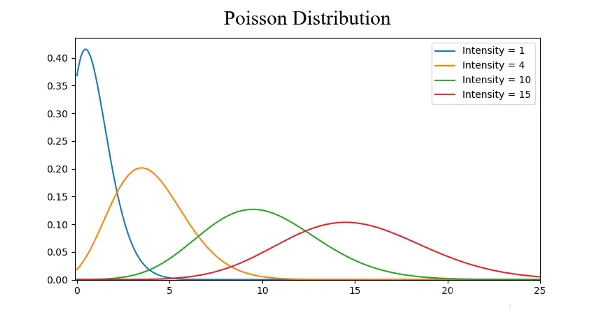
\includegraphics[width=0.55\textwidth]{figs/2022-04-27-09-17-50.png}
      \end{center}
   \[ P(X=k)=\frac{\lambda^{k}}{k !} e^{-\lambda} ; \qquad P (n) =  \frac{ \overline{n} ^{n} e^{-\overline{n}}}{n!} \]
   相干态: $ \rs{\alpha} =  D(\alpha)  \rs{0} $, 
   峰值位置: $ \overline{n} = \left| \alpha\right|^2 $, 展宽(量子涨落): $ \Delta n = \left| \alpha\right| $ 
\end{frame}

\begin{frame}
 \frametitle{场算符的量子涨落}
 \例[10.试证明所有的相干态都是最小不确定度乘积态]{
   \[ \Delta X_1 \Delta X_2 =\dfrac{1}{4} \] 
  }
 \证~湮灭算符不厄密, 总可以写成两厄密算符的如下形式
 \[ a = X_1 + i X_2, \, a ^\dagger = X_1 - i X_2, \qquad \text{with}\qquad  [X_1, X_2]= \frac{i}{2} \]
 对应场的正交分量算符: 
 \[ X_{1} =\frac{1}{2}\left(a + a^{\dagger}\right) = \sqrt{\frac{\omega}{2 \hbar} }~q\]
 \[ X_{2} = \frac{1}{2 i}\left(a - a^{\dagger}\right)= \sqrt{\frac{}{2 \hbar\omega} }~p\]
\end{frame}

\begin{frame}
 \frametitle{}
      先证明对易关系: 
    \[ \begin{aligned}
        \hat{X}_{1} \hat{X}_{2} & =\mathrm{i}\left(\hat{a}^{\dagger}+\hat{a}\right)\left(\hat{a}^{\dagger}-\hat{a}\right) / 4\\ 
        &=\mathrm{i}\left(\hat{a}^{\dagger} \hat{a}^{\dagger}+\hat{a} \hat{a}^{\dagger}-\hat{a}^{\dagger} \hat{a}-\hat{a} \hat{a}\right) / 4 \\ 
        \hat{X}_{2} \hat{X}_{1} & = \mathrm{i}\left(\hat{a}^{\dagger}-\hat{a}\right)\left(\hat{a}^{\dagger}+\hat{a}\right) / 4 \\ 
        & =\mathrm{i}\left(\hat{a}^{\dagger} \hat{a}^{\dagger}-\hat{a} \hat{a}^{\dagger}+\hat{a}^{\dagger} \hat{a}-\hat{a} \hat{a}\right) / 4 \\ 
        \left[\hat{X}_{1}, \hat{X}_{2}\right] & =\hat{X}_{1} \hat{X}_{2}-\hat{X}_{2} \hat{X}_{1} \\ 
        &= \mathrm{i}\left(\hat{a} \hat{a}^{\dagger}-\hat{a}^{\dagger} \hat{a}\right) / 2 \\ 
        & =\mathrm{i}\left[\hat{a}, \hat{a}^{\dagger}\right] / 2  \\ &=  \frac{i}{2} \\ 
        \Delta X_1 \Delta X_2 & \geq  \left| \left[\hat{X}_{1}, \hat{X}_{2}\right]  \right| /2  \\ 
        &= \frac{1}{4}
    \end{aligned}\]

\end{frame}

\begin{frame} 
 \frametitle{}
      电场的行波展开
      \[ \begin{aligned}
          E(\mathbf{r},t)  &= i  \sqrt{\frac{\hbar \omega}{2 \epsilon_0 V}} [a e^{i(\mathbf{k}\cdot \mathbf{r} -\omega t) }- 
          a^{\dagger} e^{-i(\mathbf{k}\cdot \mathbf{r}-\omega t)}]\\
          &=i  \sqrt{\frac{\hbar \omega}{2 \epsilon_0 V}} [X_1 \sin(\mathbf{k}\cdot \mathbf{r}-\omega t) + X_2 \cos(\mathbf{k}\cdot \mathbf{r}-\omega t)] 
      \end{aligned}\] 
      电场的驻波展开
      \[ \begin{aligned}
        E(\mathbf{r},t)  &= \frac{1}{2} E_0 [ a e^{ -\omega t}+ a^{\dagger} e^{ \omega t}] \\ 
        &= E_0 [X_1 \cos(\omega t)+ X_2 \sin(\omega t)]
      \end{aligned}\]
    式中
    \[ X_1 = \sqrt{\frac{\omega}{2\hbar}}q, \qquad X_2 = \sqrt{\frac{1}{2\hbar\omega}}p\]
\end{frame}
\begin{frame} 
    对相干态求均值
    \[
    \begin{aligned}
        \overline{ X_1}  &= \lcr{\alpha}{\frac{1}{2}\left(a+a^{\dagger}\right)}{\alpha} = \frac{1}{2}(\alpha+\alpha^*) \\
        \overline{X_2}  &= \lcr{\alpha}{\frac{1}{2i}\left(a-a^{\dagger}\right)}{\alpha} = \frac{1}{2i}(\alpha-\alpha^*) \\
    \end{aligned}\]
    对相干态求方的均值
    \[
    \begin{aligned}
      \overline{X^2 _1} &= \lcr{\alpha}{\frac{1}{4}\left(a+a^{\dagger}\right)^2} {\alpha}  \\ 
      &= \frac{1}{4}\lcr{\alpha}{\left(aa+a^{\dagger}a^{\dagger}+ aa^{\dagger} + a^{\dagger}a\right)} {\alpha}  \\
      &= \frac{1}{4}\lcr{\alpha}{\left(aa+a^{\dagger}a^{\dagger}+ 2a^{\dagger}a + 1 \right)} {\alpha} \\
      &= \frac{1}{4}(\alpha + \alpha^*)^2+ \frac{1}{4}
    \end{aligned}   
    \]
\end{frame}

\begin{frame}
      \frametitle{}
      \[
        \begin{aligned}
          \overline{X^2 _2} &= \lcr{\alpha}{-\frac{1}{4}\left(a-a^{\dagger}\right)^2} {\alpha}  \\ 
          &= -\frac{1}{4}\lcr{\alpha}{\left(aa+a^{\dagger}a^{\dagger}- aa^{\dagger} - a^{\dagger}a\right)} {\alpha}  \\
          &= -\frac{1}{4}\lcr{\alpha}{\left(aa+a^{\dagger}a^{\dagger}- 2a^{\dagger}a - 1 \right)} {\alpha} \\
          &= -\frac{1}{4}(\alpha - \alpha^*)^2 + \frac{1}{4}
        \end{aligned}   
        \]  
        求场的量子涨落:
        \[ \Delta X_1 = \sqrt{\overline{X^2 _1}- \overline{X_1}^2} = \frac{1}{2}\]
        \[ \Delta X_2 = \sqrt{\overline{X^2 _2}- \overline{X_2}^2} = \frac{1}{2}\]
        \[ \Delta X_1 \Delta X_2=\frac{1}{4}\]
    证毕!
\end{frame}

\begin{frame} 
\frametitle{相干态的相位分布}
对于相干态$\rs{\alpha}$, 取
\[ \alpha = \left|\alpha\right| e^{i\theta}\]
相位分布:
    \[\begin{aligned}
    P(\varphi) &=\frac{1}{2\pi} \left| \lr{\varphi}{\alpha} \right|^2 \\ 
    &= \frac{1}{2\pi} e^{-\left|\alpha\right|^2} \left|  \sum_{n=0} ^{+\infty}  e^{i[n(\varphi-\theta)]}\frac{|\alpha|^n}{\sqrt{n!}} \right|^2
    \end{aligned} \] 
当 $|\alpha|^2$很大时, 泊松分布可近似为高斯分布
\[ e^{-\left|\alpha\right|^2 /2}\frac{|\alpha|^{2n}}{n!} e^{-\left|\alpha\right|^2} \approx \frac{1}{\sqrt{2\pi \left|\alpha\right|^2}} \exp[-\frac{(n-\left|\alpha\right|^2)^2}{2\left|\alpha\right|^2}]\]   
\end{frame}

\begin{frame}
\frametitle{}
\begin{columns}
    \begin{column}[t]{0.6\linewidth}
        ~\\
    相位近似为峰位在$\varphi = \theta$处的高斯分布:
        \[ P(\varphi) \approx \sqrt{\frac{2 \left|\alpha\right|^2}{\pi}} \exp[-2\left|\alpha\right|^2(\varphi - \theta)^2]\]
   很明显,随着 $\left|\alpha\right|^2$的增大, 相位分布集中到$\varphi = \theta$附近。即相位变得越来越确定, 相干态趋相于经典态。
    \end{column}
    \begin{column}[t]{0.4\linewidth} 
          \begin{center}
               
\includegraphics[width=1.0\textwidth]{figs/33.png} 
          \end{center} 
    \end{column} 
\end{columns} 
\end{frame}

\begin{frame}
      \frametitle{相干态的相图}
    与真空态不同, 相干态的场矢量大小为$\left|\alpha\right|$, 是平移量的模! 
   \begin{center}
        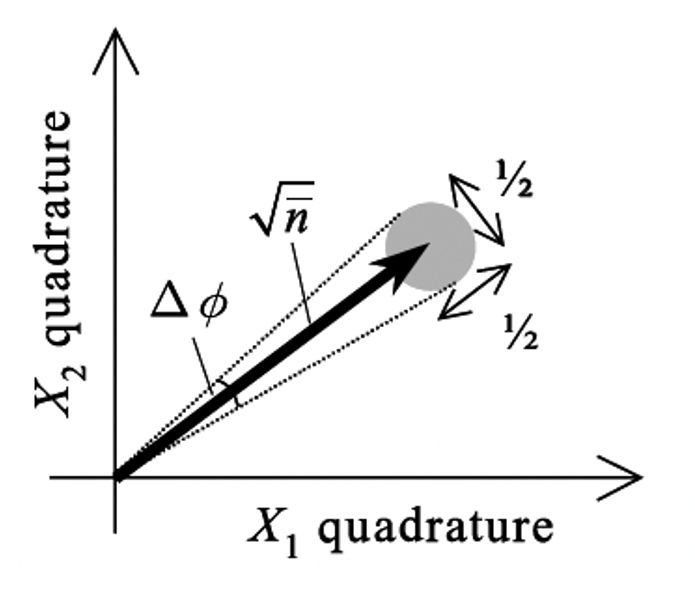
\includegraphics[width=0.35\textwidth]{figs/13.png}
   \end{center}
   相干态是真空态的幺正平移,因此涨落性质不变!\\ 
   但随着场强增大,其相位的不确定度从真空态的无限大变得越来越小,\\ 当场强足够大时, 相位的不确定度趋零,对应于有确定相位的经典电磁场.
\end{frame}

\begin{frame}
    \frametitle{相干态的产生}
  理论上,得要构造一个系统, 具有如下平移算符. 
  \[ D(\alpha)=\exp \left(\alpha a^{\dagger}-\alpha^{*} a\right) \]
  ~\\ {\vspace*{2.3em}} 
  实验上:\\
  (1)电流源辐射: 激发(平移)真空态产生相干辐射场.
\end{frame}

\begin{frame}
    ~\\
   (2)原子受激辐射: 大量同一种原子受激辐射, 产生与激源光子物理特性完全相同的光(激光).  
     \begin{center}
      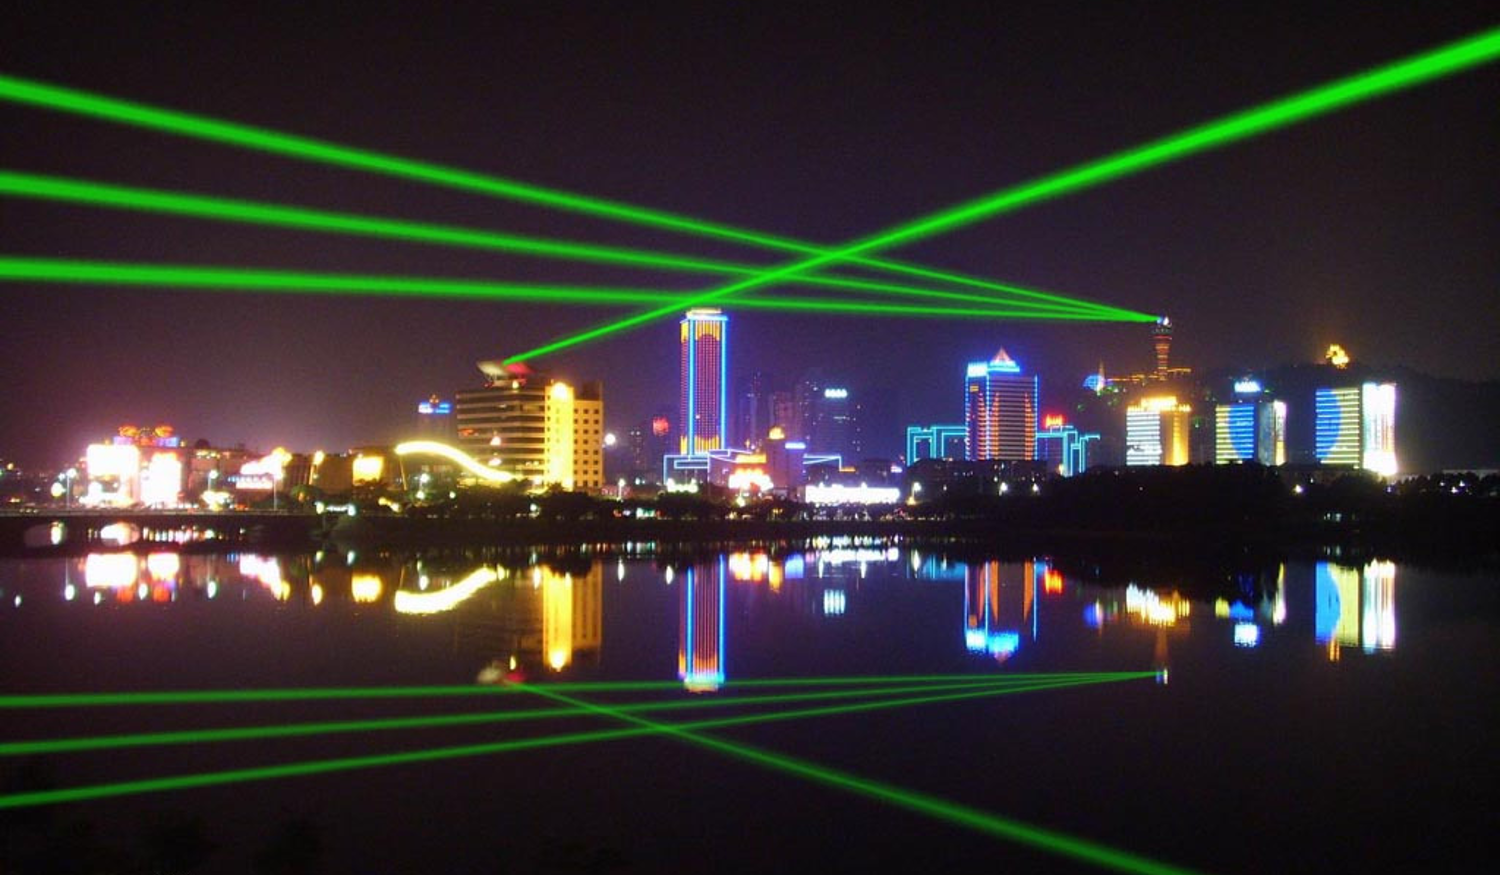
\includegraphics[width=0.35\textwidth]{figs/8.png}
    \end{center}   
 原子自发辐射发的光子,不具有相位、偏振态、传播方向上的一致性,是非相干光. 当有信号光子入射时, 处于高能级的原子可辐射一个与信号光子频率、相位、偏振态以及传播方向都相同的光子. 如果大量原子被激励(平移)到高能级,则可产生大量频率、相位、偏振态以及传播方向相同的相干光.  
\end{frame}

\begin{frame}
    \frametitle{相干态随时间的演化规律}
        \例[11. 已知$t=0$时刻的相干态为$\rs{\alpha (0)}$, 试求t时刻的相干态$\rs{\alpha (t)}$  ]{}
        \解 ~ 设光场哈密顿不显含时间, 其时间演化算符为
    \[ \begin{aligned}
     \hat{U}(t, 0)  &= e^{-i \hat{H}t / \hbar}\\ 
     &= e^{-i \hbar \omega ( a^\dagger a+\frac{1}{2} ) t / \hbar} \\ 
     &= e^{-i \omega t (a^\dagger a +\frac{1}{2} )}  \\ 
    \end{aligned}\]
    数态表象:
    \[ \begin{aligned}
        \rs{\alpha (t)} &= \hat{U}(t, 0) \rs{\alpha (0)} \\ 
        &= e^{-i \omega t ( a^\dagger a +\frac{1}{2} )} \rs{\alpha (0)} \\ 
        &= e^{-i \omega t ( a^\dagger a +\frac{1}{2} )} e^{-\frac{1}{2}\left|\alpha(0)\right|^2}  \sum_{n=0} ^{+\infty}  \frac{\alpha(0)^n}{\sqrt{n!}} \rs{n}  \\  
       \end{aligned}\]
\end{frame}

\begin{frame}
    \frametitle{}
    \[ \begin{aligned}
        \rs{\alpha (t)} &= e^{-i\frac{1}{2} \omega t}  e^{-\frac{1}{2}\left|\alpha(0)\right|^2} \sum_{n=0} ^{+\infty}  \frac{\alpha(0)^n}{\sqrt{n!}} e^{-i \omega t  a^\dagger a}  \rs{n}  \\
        &= e^{-i\frac{1}{2} \omega t}  e^{-\frac{1}{2}\left|\alpha(0)\right|^2}\sum_{n=0} ^{+\infty}  \frac{\alpha(0)^n}{\sqrt{n!}} e^{-i n \omega t }  \rs{n}  \\ 
        &= e^{-i\frac{1}{2} \omega t}  e^{-\frac{1}{2}\left|\alpha(0)\right|^2} \sum_{n=0} ^{+\infty}  \frac{(\alpha(0) e^{-i \omega t })^n}{\sqrt{n!}} \rs{n}  \\ 
        &= e^{-i\frac{1}{2} \omega t} e^{\left|e^{-i \omega t }\right|^2}   e^{-\frac{1}{2}\left|\alpha(0)e^{-i \omega t }\right|^2} \sum_{n=0} ^{+\infty}  \frac{(\alpha(0) e^{-i \omega t })^n}{\sqrt{n!}} \rs{n}  \\ 
        &= e^{-i\frac{1}{2} \omega t}  e^{\left|e^{-i \omega t }\right|^2}  \rs{\alpha(0) e^{-i \omega t} } \\ 
        &= \rs{\alpha(0) e^{-i \omega t}} \\ 
       \end{aligned}\]
\end{frame}

\begin{frame}
      \frametitle{}
      \[ \rs{\alpha (t)}= \rs{\alpha(0) e^{-i \omega t}}  \]
       说明: 随着时间的推移, 相干态的本征值只是获得一个相位 $e^{-i \omega t}$, 相干态本身变成了湮灭算符的属于本征值$ \alpha(0) e^{-i \omega t} $的本征态. \\ {\vspace*{0.6em}} 
       即, 随着时间的推移, 相干态只是获得一个相位振荡, 它还是湮灭算符的本征态, 所以相干特性不随时间发生变化. 这正是实验上发现稳定相干条纹的前提.
\end{frame}

\begin{frame} 
\frametitle{}
     数态在正则位置表象中的波函数
     \[\left\langle q|n \right\rangle = (2^n n!)^{-1/2} ( \frac{\omega}{\pi \hbar})^{1/4} \exp(-\xi^2 /2) H_n (\xi), \quad \text{with}~~ \xi= q/\sqrt{\omega/\hbar}\]
     相干态在正则位置表象中的波函数
     \[\begin{aligned}
         \left\langle q| \alpha \right\rangle & = \left\langle q \left| e^{-\frac{1}{2}\left|\alpha\right|^2}  \sum_{n=0} ^{+\infty}  \frac{\alpha^n}{\sqrt{n!}} \right| n \right\rangle \\
         &=( \frac{\omega}{\pi \hbar})^{1/4} e^{-|\alpha|^2 /2} e^{\xi^2 /2} e^{-(\xi - \alpha/\sqrt{2})^2}  \\
     \end{aligned}\] 
    因此,t时刻的波函数为: 
    \[\psi_\alpha (q,t) = \left\langle q| \alpha(t) \right\rangle = ( \frac{\omega}{\pi \hbar})^{1/4} e^{-|\alpha|^2 /2} e^{\xi^2 /2} e^{-(\xi - \alpha e^{-i \omega t/\sqrt{2}})^2} \]
    是一个中心位置随时间振荡的高斯函数!(频率$\omega/\sqrt{2}$)
\end{frame}

\begin{frame} 
    \frametitle{}
        \begin{center}
        \animategraphics[height=2in,loop]{30}{gif/test-}{1}{80} 
        \end{center} 
    相干态在正则位置表象表现为: 
    \begin{enumerate}
      \item 波包的形状保持不变
      \item 在中心位置附近做周期性振荡
    \end{enumerate}  
    \end{frame}

\begin{frame}
 \frametitle{}
    \begin{center}
    \animategraphics[height=2in,loop]{30}{gif/coh-}{1}{100} 
    \end{center}
    相干态在相图中表现为:
 \begin{enumerate}
     \item 场矢大小保持不变
     \item 相位随时间发生周期性振荡(频率$\omega$)
 \end{enumerate}
\end{frame}

\section{5. 相干态表象}

\begin{frame}
    \frametitle{相干态不正交}
        \例[12.试证明相干态不具正交性]{}
        \证 ~ 相干态
        \[\rs{\alpha}=e^{-\frac{1}{2}\left|\alpha\right|^2}  \sum_{n=0} ^{+\infty}  \frac{(\alpha\hat{a}^\dagger)^n}{n!}\rs{0} \] 
    代入内积公式
    \[ \begin{aligned}
     \lr{\alpha}{\beta} &= \lr{0\left|\sum_{n=0} ^{+\infty}\frac{(\alpha\hat{a}^\dagger)^n}{n!}}{\sum_{n=0} ^{+\infty}\frac{(\beta\hat{a}^\dagger)^n}{n!}\right|0} e^{-\frac{1}{2}(\left|\alpha\right|^2 +\left|\beta\right|^2)}\\ 
     &= e^{-\frac{1}{2}(\left|\alpha\right|^2 +\left|\beta\right|^2)} \sum_{n=0} ^{+\infty}\frac{(\alpha^*)^n (\beta)^n}{n!} \\ 
     &= e^{\alpha^* \beta -\frac{1}{2}(\left|\alpha\right|^2 +\left|\beta\right|^2)} \\ 
     \left|\lr{\alpha}{\beta} \right|^2 &= e^{-  \left| \alpha - \beta\right|^2} \not = 0 
    \end{aligned}\]
\end{frame}

\begin{frame}
    Analysing the two-slit experiment:
      \begin{center}
           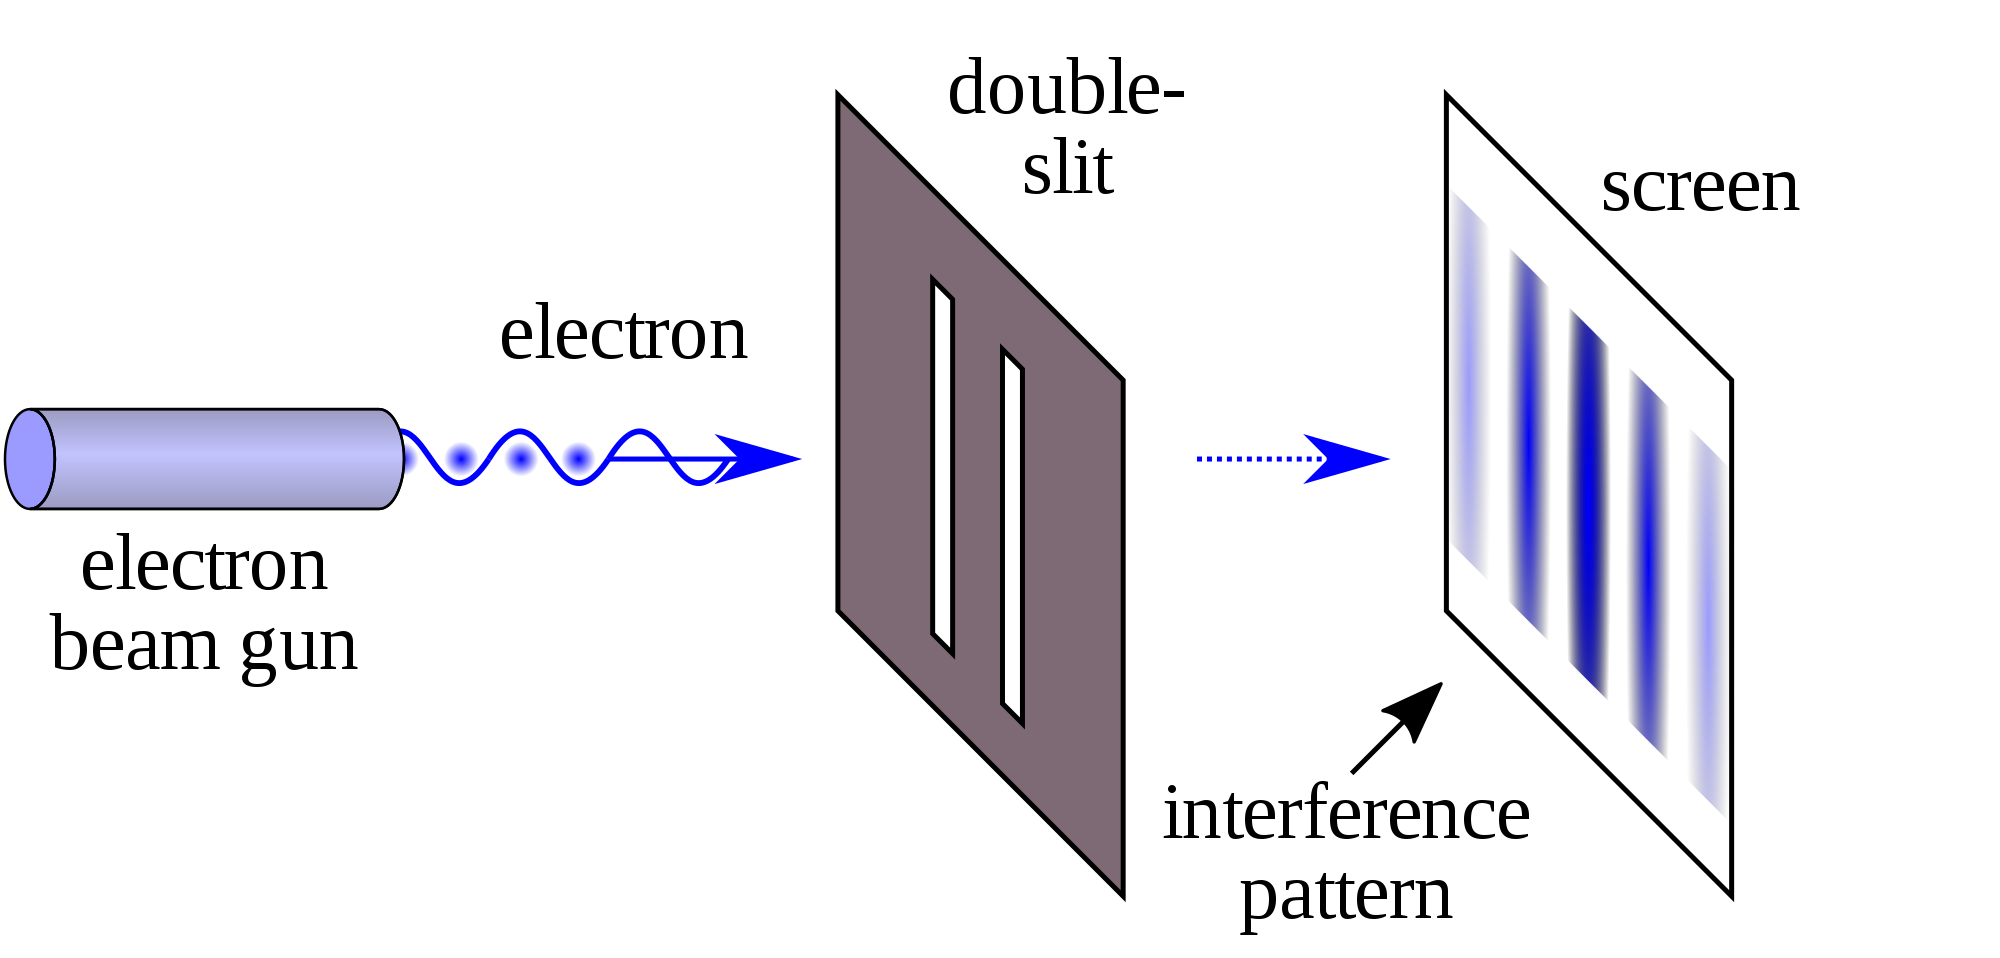
\includegraphics[width=0.6\textwidth]{figs/Etwoslitexp.png}
      \end{center}
    \begin{itemize}
        \Item Using wavefunction $\rs{\psi_1}$ to describe the state of the electron running across slit-1 and $\rs{\psi_2}$ for slit-2. when the both slits opened, the electron locates at the superposition state
            \[ \rs{\Psi}=c_1 \rs{\psi_1}+ c_2\rs{\psi_2} \]
    \end{itemize}
\end{frame}

\begin{frame}
    \tikzstyle{na} = [baseline=-.5ex]
    \begin{itemize}
        \Item based on statistical interpretation, the possiblity density of electron reaches certain point of screen should be
        \begin{equation*}
        \begin{split}
            \omega &=|\rs{\Psi}|^2 \\
            &= (\ls{\psi_1}c_1 + \ls{\psi_2}c_2 ) (c_1 \lr{\psi_1}+ c_2\lr{\psi_2}) \\
            & = |c_1|^2 |\rs{\psi_1}|^2 + |c_2|^2 |\rs{\psi_2}|^2  
            + \Myitem{t1}{red}{c_1 c_2 ^* \lr{\psi_2}{\psi_1} + c_1 ^* c_2 \lr{\psi_1}{\psi_2} } \\
        \end{split} 
        \end{equation*}
    \end{itemize}
    \begin{itemize}
        \Item 存在相干项(后两项),形成干涉条纹
        \Item 相干项不为零的条件: 
        \begin{enumerate}
            \item 叠加态: 即同时过两个缝, 否则有$\psi_1$ 或$\psi_2$为零,相干项为零
            \item 不正交性: $\rs{\psi_1}$与 $\rs{\psi_2}$不正交, 否则相干项为零
        \end{enumerate}
        \Item $\left|\lr{\alpha}{\beta} \right|^2 = e^{-  \left| \alpha - \beta\right|^2}$ 表明, 当$\alpha - \beta \to \infty $, 
        趋于正交, 相干项趋零.
    \end{itemize}
\end{frame}

\begin{frame}
 \frametitle{}
   \begin{center}
        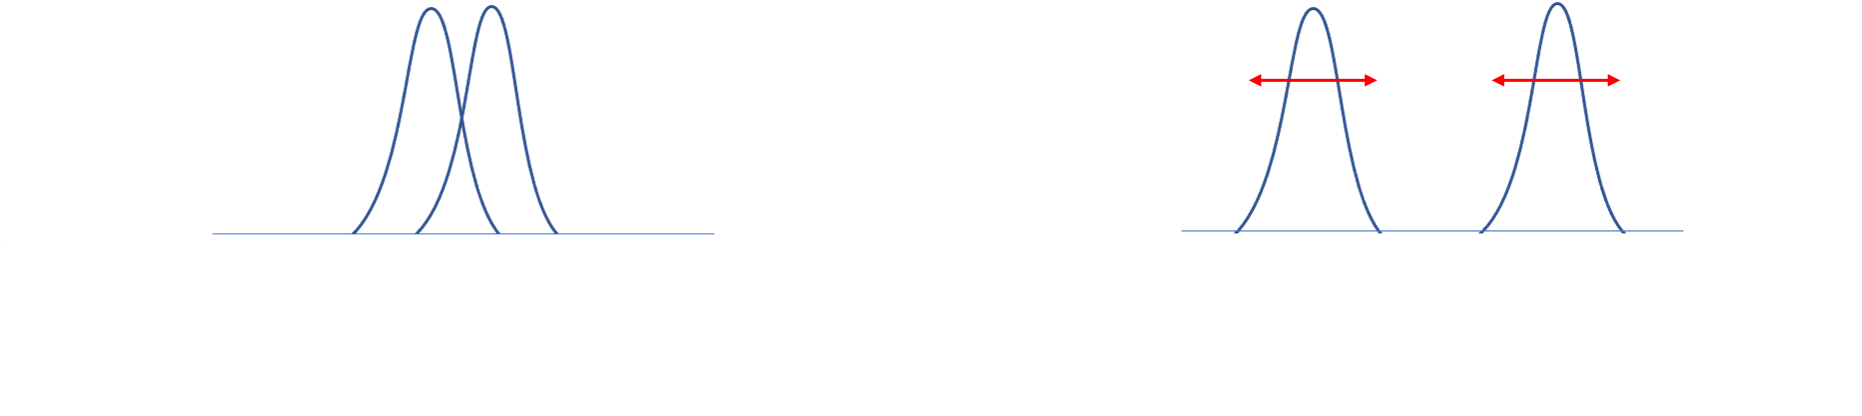
\includegraphics[width=1.0\textwidth]{figs/11.png}
   \end{center}
 当$\alpha - \beta \to \infty $, 两位移量差别大, 两波函数虽不正交但振荡过程中相互重叠部分趋零, 因此内积趋零, 干涉项趋零, 干涉条纹变弱趋无。
 
\end{frame}

\begin{frame}
 \frametitle{相干态的超完备性}
 \例[13.试证明相干态具有如下完备性关系]{
    \[ \frac{1}{\pi} \int \rl{\alpha}{\alpha}d ^2 \alpha =1 \] }
 \证 ~ 把相干态的数态展开式
    \[\rs{\alpha} = e^{-\frac{1}{2}\left|\alpha\right|^2}  \sum_{n=0} ^{+\infty}  \frac{\alpha^n}{\sqrt{n!}} \rs{n} \]
 代入上式左边:
 \[
    \begin{aligned}
        \frac{1}{\pi} \int \rl{\alpha}{\alpha}d ^2 \alpha &=  \frac{1}{\pi} \int \sum_{n,m=0} ^{+\infty} e^{-\left|\alpha\right|^2}  
        \frac{\alpha^n(\alpha^*)^m}{\sqrt{n!m!}}  \rs{n}\ls{m }d ^2 \alpha \\
        &= \sum_{n,m=0} ^{+\infty}  \frac{\rs{n}\ls{m }}{\pi \sqrt{ n!m!}}  \int  e^{-\left|\alpha\right|^2}  \alpha^n(\alpha^*)^m  d ^2 \alpha
    \end{aligned}    
 \]    
\end{frame}

\begin{frame}
 \frametitle{}
  转换到极坐标系进行计算
  \[ 
    \begin{aligned}
        \frac{1}{\pi} \int \rl{\alpha}{\alpha}d ^2 \alpha 
        &= \sum_{n,m=0} ^{+\infty}  \frac{\rs{n}\ls{m }}{\pi \sqrt{ n!m!}}  \int  e^{-\left|\alpha\right|^2}  \alpha^n(\alpha^*)^m  d ^2 \alpha \\ 
        &= \sum_{n,m=0} ^{+\infty}  \frac{\rs{n}\ls{m }}{\pi \sqrt{ n!m!}} 
        \int _0 ^ {+\infty}  e^{-r^2}  r^{n+m}  r dr   \int _0 ^ {2 \pi} e^{i(n-m)\theta} d\theta  \\ 
        &= \sum_{n,m=0} ^{+\infty}  \frac{\rs{n}\ls{m }}{\pi \sqrt{ n!m!}} 
        \int _0 ^ {+\infty}  e^{-r^2}  r^{n+m}  r dr   2 \pi \delta(n-m)  \\ 
        &= \sum_{n=0} ^{+\infty}  \frac{\rs{n}\ls{n }}{\sqrt{ n!n!}} 
        \int _0 ^ {+\infty}  e^{-r^2}  r^{n+n}  2r dr  \\ 
        &= \sum_{n=0} ^{+\infty}  \frac{\rs{n}\ls{n }}{n!} 
        \int _0 ^ {+\infty}  e^{-(r^2)}  (r^2)^{n}   d(r^2)  
    \end{aligned}    
 \]        
\end{frame}

\begin{frame}
 \frametitle{}
 \[ 
    \begin{aligned}
        \frac{1}{\pi} \int \rl{\alpha}{\alpha}d ^2 \alpha    
        &= \sum_{n=0} ^{+\infty}  \frac{\rs{n}\ls{n }}{n!} 
        \int _0 ^ {+\infty}  e^{-t}  t^n   dt  \\ 
        &= \sum_{n=0} ^{+\infty}  \frac{\rs{n}\ls{n }}{n!} 
        \Gamma(n+1)  \\ 
        &= \sum_{n=0} ^{+\infty}  \frac{\rs{n}\ls{n }}{n!} 
        n!  \\ 
        &= \sum_{n=0} ^{+\infty}  \rs{n}\ls{n } \\
        &= 1
    \end{aligned}    
 \] 
 证毕!
\[  \boxed{ \frac{1}{\pi} \int \rl{\alpha}{\alpha}d ^2 \alpha =1} \]
\end{frame}

\begin{frame} 
\frametitle{}
     * 相干态表象的过完备性: $\{\rs{\alpha}\}$的一个子集就可以构成一组完备基, 因此一个态函数在相干态表象中的展开系数是不唯一的.也称超完备性. \\ {\vspace*{0.3em}}
     \证~(1)线性不独立性
     \[ \begin{aligned}
         \int \alpha ^m \rs{\alpha} d^2 \alpha &= \sum_n \frac{\rs{n}}{\sqrt{n!}} \int_0 ^\infty \left|\alpha\right|^{n+m+1} e ^ {- \left|\alpha\right|^2 /2} \int_0 ^{2\pi} e ^{i(n+m)\varphi}  d \varphi =0\\
     \end{aligned}\] 
     (2) 相干态可以相互展开
     \[ \begin{aligned}
        \rs{ \beta } & = \frac{1}{\pi} \int \rs{\alpha} \left\langle \alpha | \beta \right\rangle  d ^2 \alpha \\ 
        &= \frac{1}{\pi} \int \rs{\alpha} e^{-  \left| \alpha - \beta\right|^2}  d ^2 \alpha
    \end{aligned}\] 
\end{frame}

\begin{frame} 
\frametitle{}
     (3) 对于$\{\rs{\alpha}\}$,设$\alpha = r e ^{i \varphi}$, 则$r$取一个固定值的子集就是一组完备基
      \[ \begin{aligned}
          \int _0 ^{2\pi} \rs{\alpha} e ^{-i m \varphi} d \varphi &= e^{- r^2 /2 \sum_n \frac{\rs{n} r^n}{\sqrt{n!}} } \int _0 ^{2\pi} e ^{i (n-m) \varphi} d \varphi \\
          &= 2\pi r^m e^{- r^2 /2}  \frac{\rs{m}}{\sqrt{m!}} \\
        \to \rs{m} &= \frac{r^{-m}}{2\pi}e^{ r^2 /2}  \int _0 ^{2\pi} \rs{\alpha} e ^{-i m \varphi} d \varphi 
      \end{aligned}\] 
      数态可以在这个子集上展开, 因此是完备的. 
\end{frame}

\begin{frame} 
\frametitle{}
      (4) 算符在相干态表象中的矩阵表示是不唯一的.
    \[\begin{aligned}
         F_{\alpha' \alpha} &= \left\langle \alpha' | F |\alpha \right\rangle \\ 
         &= \sum_m \sum_n  \left\langle \alpha' |m \right\rangle F_{mn} \left\langle n |\alpha \right\rangle \\
         &= F(\alpha^*, \alpha')e^{-(\left|\alpha\right|^2+ \left|\alpha'\right|^2)/2}  
    \end{aligned} \]
      式中 \[F(\alpha^*, \alpha')= \sum_m \sum_n F_{mn} \frac{(\alpha^*)^m (\alpha)^n}{\sqrt{m! n!}}\]
     称矩阵元的生成函数.
\end{frame}

\begin{frame} 
\frametitle{}
    (5)对角元已具有完全性 \\ {\vspace*{0.6em}}
      上式取$\alpha'=\alpha$, 得相干态表象矩阵的对角元。
      \[ \left\langle \alpha|F|\alpha \right\rangle\]
      通过这些对角元即可生成数态表象中的整个矩阵
      \[ \left\langle \alpha|F|\alpha \right\rangle e^{\alpha^* \alpha} = \sum_m \sum_n  \frac{(\alpha^*)^m (\alpha)^n}{\sqrt{m! n!}} \left\langle m|F|n \right\rangle\]
\end{frame}

\begin{frame} 
 \frametitle{}
        \begin{center}
             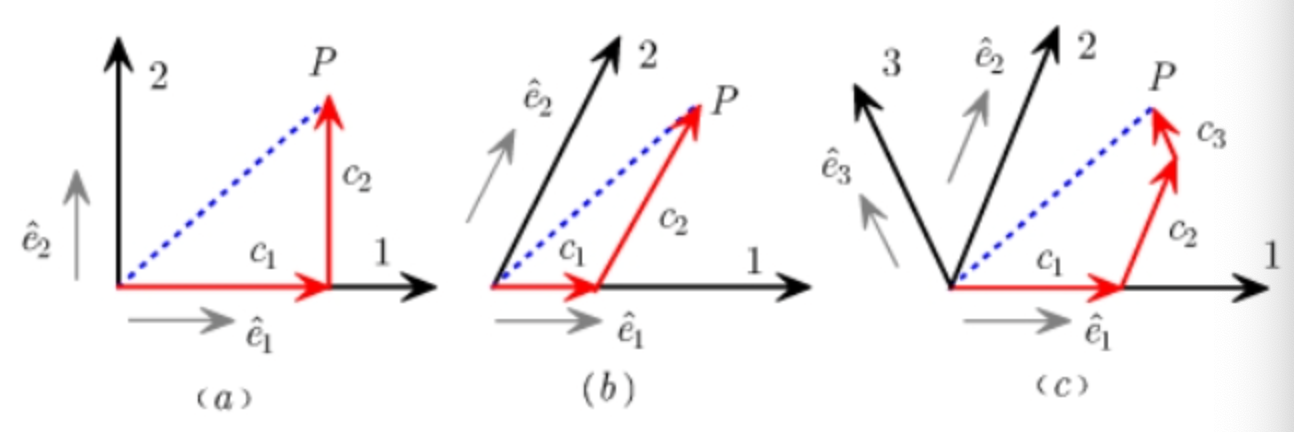
\includegraphics[width=1.0\textwidth]{figs/2022-05-11-11-10-06.png}
        \end{center}
    \begin{enumerate}
        \item 正交完备空间~表述唯一
        \item 非正交完备空间~表述唯一
        \item 非正交超完备空间~表述不唯一
    \end{enumerate}
\end{frame}

%%%%%%%%%%%%%%%%%%%%%%%%%%%%%%%%%%%%%%%%%%%%%%%%%%%%%%%%%%%%%%%%%%%
\begin{frame}
    \frametitle{课外作业}
    \begin{enumerate}
        \item 试证明相干态是最小不确定度乘积态
        \item 试求相干态在正则位置表象中的波函数
        \[\left\langle q| \alpha \right\rangle = ( \frac{\omega}{\pi \hbar})^{1/4} e^{-|\alpha|^2 /2} e^{\xi^2 /2} e^{-(\xi - \alpha/\sqrt{2})^2}  , \quad \text{with}~~ \xi= \frac{q}{\sqrt{\omega/\hbar}}\]
        \item 试求正则位置表象中相干态随时间的振荡表达式
        \item 证明
        \[D^\dagger (\alpha) a^\dagger D (\alpha) = a^\dagger + \alpha^* \]
        \[ \rs{\alpha }\ls{\alpha } a= \left( \alpha + \frac{\partial }{\partial \alpha^*} \rs{\alpha }\ls{\alpha } \right)\]
    \end{enumerate}
\end{frame}
%%%%%%%%%%%%%%%%%%%%%%%%%%%%%%%%%%%%%%%%%%%%%%%%%%%%%%%%%%%%%%%%%%    % 相干态
%%%%%%%%%%%%%%%%%%%%%%%%%%%%%%%%%%%%%%%%%%%%%%%%%%%%%%%%%%%%%%
\begin{frame} [plain]
    \frametitle{}
    \Background[1] 
    \begin{center}
    {\huge 第8-9讲:压缩态}
    \end{center}  
    \addtocounter{framenumber}{-1}   
\end{frame}
%%%%%%%%%%%%%%%%%%%%%%%%%%%%%%%%%%%%%%%%%%%%%%%%%%%%%%%%%%%% 

\section{1. 压缩态基本概念}

\begin{frame}
    \frametitle{}
    \begin{tcolorbox3}[前情回顾]
     \begin{itemize}
                \item 真空态是最小不确定度乘积态
                \item 相干态也是小不确定度乘积态
                \[ \Delta X_1 \Delta X_2 =\dfrac{1}{4}, \, \Delta X_1 = \Delta X_2 = \frac{1}{2} \] 
         \end{itemize}
    \end{tcolorbox3}
\end{frame}

\begin{frame}
 \frametitle{}
      \begin{center}
           \begin{tcolorbox2}[0.86]{压缩态的定义:}
            某正交分量的涨落被压缩的最小不确定度乘积态($\Delta X_i < \dfrac{1}{2}$)
            \[ \Delta X_1 \Delta X_2 =\dfrac{1}{4}, \, \Delta X_1 \not = \Delta X_2  \] 
            \centering
            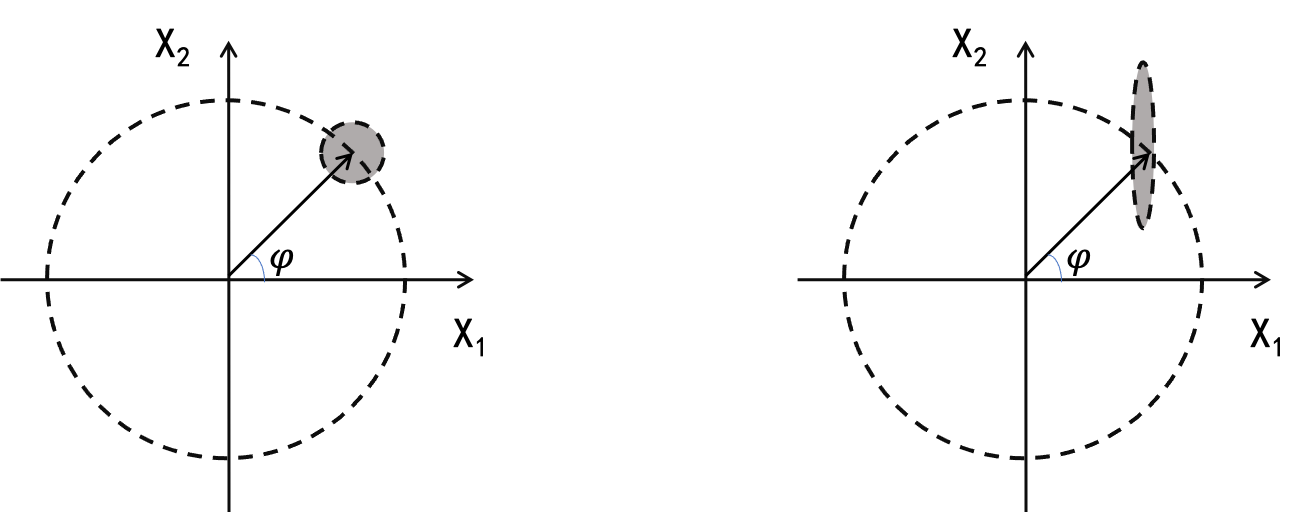
\includegraphics[width=0.66\textwidth]{figs/6.png}
          \end{tcolorbox2}  
      \end{center} 
\end{frame}

\begin{frame}
 \frametitle{}
 发展与影响:
 \begin{itemize}
     \item  1970年 D. Stoler[1], 提出压缩相干态概念。
     \item  1980年 压缩态得以实现并发展到最高可压缩80\%
     \item  随后逐渐应用到各种精密测量和量子通讯, 并在引力波测量中大显身手 
     \item 基此衍生的纠缠光子对技术,也已成为量子加密和量子计算的重要基础。
 \end{itemize}
 ~~ \\ {\vspace*{2.8em}}
 (1) D. ~Stoler, Phys. Rev.  A ~ 131, 2766(1970)    
\end{frame}

\begin{frame}
 \frametitle{谐振子基态的平移与压缩}
 谐振子哈密顿
 \[  H= \frac{p^2}{2m} +\frac{1}{2}m \omega^2 q^2\]
 作如下变化, 试求解谐振子 
 \[ (1) ~~H= \frac{p^2}{2m} +\frac{1}{2}m \omega^2 q^2 +c \]
 \[ (2) ~H= \frac{p^2}{2m} +\frac{1}{2}m \omega^2 q^2 +cq\]
 \[ (3) H= \frac{p^2}{2m} +\frac{1}{2}m \omega^2 q^2 +cq^2\]
 \end{frame}
 
 \begin{frame}
       \frametitle{}     
  \解 (1) 
    \[\begin{aligned}
    H &= \frac{p^2}{2m} +\frac{1}{2}m \omega^2 q^2 +c \\  
    H-c &= \frac{p^2}{2m} +\frac{1}{2}m \omega^2 q^2  \\ 
    H' &= \frac{p^2}{2m} +\frac{1}{2}m \omega^2 q^2  \\  
    H' &=\hbar \omega (n+\frac{1}{2}) \\ 
    H &= \hbar \omega (n+\frac{1}{2}) +c
    \end{aligned} \]  
* 基态能平移至 $\dfrac{1}{2}\hbar \omega + c$ \\ 
* 谐振子能级发生整体平衡, 不影响波包的形态.   
\end{frame}

\begin{frame}
 \frametitle{}
 (2) 

   \[\begin{aligned}
    H &= \frac{p^2}{2m} +\frac{1}{2}m \omega^2 q^2 +cq \\ 
    H-c_2 &= \frac{p^2}{2m} +\frac{1}{2}m \omega^2 (q+c_1)^2  \\ 
    H' &= \frac{p^2}{2m} +\frac{1}{2}m \omega^2 (q')^2  \\ 
   \end{aligned} \]    
  
 * 能级和位置都发生整体平移, 不影响谐振子基态波包的形态 \\ 
 * 基态位置的平移,导致相干态的产生。
\end{frame}

\begin{frame}
 \frametitle{}
  (3)  
    \[\begin{aligned}
        H &= \frac{p^2}{2m} +\frac{1}{2}m \omega^2 q^2 +cq^2 \\ 
        H &= \hbar \omega (a^\dagger a +\frac{1}{2}) +cq^2  \\ 
        H  &= \hbar \omega (a^\dagger a +\frac{1}{2}) +c \frac{\hbar}{2m \omega} (a^2 + a^{\dagger 2} + 2 a^\dagger a +1 ) \\ 
        H-c_2 &= c_0\hbar \omega (a^\dagger a +\frac{1}{2}) +c_1 (a^2 + a^{\dagger 2})  \\ 
        H' &= c_0\hbar \omega (a^\dagger a +\frac{1}{2}) +c_1 (a^2 + a^{\dagger 2})  \\ 
    \end{aligned} \]    
    * 这是一个收缩的势阱。\\
    * 增加的$a^2$ 和 $a^{\dagger 2}$ 涉及到光子的二次产生和湮灭过程, 谐振子基态波包的形态发生变化,导致压缩态的产生。
\end{frame}

\begin{frame}
 \frametitle{}  
 {\Bullet}考虑如下哈密顿 
 \[\begin{aligned}
     H &= \frac{(p/\xi)^2}{2m} +\frac{1}{2}m \omega^2 (\xi q)^2  \\ 
 \end{aligned} \]    
 直接对正则位置和动量进行了伸缩操作, 因此求解过程与原来的完全一样. 基态还是最小不确定度乘积态
 \[ \Delta X_1 \Delta X_2 =\dfrac{1}{4}\] 
 但涨落却变为 
 \[ \Delta X_1  = \frac{1}{2 \xi^2}, \, \Delta X_2  = \frac{\xi^2}{2}\]  
 当$\left|\xi\right|>1$, 是对 $X_1 $ 的压缩. 当$\left|\xi\right|<1$, 是对 $X_2 $ 的压缩. 
\end{frame}

\section{2. 压缩算符}

\begin{frame}
 \frametitle{压缩算符的定义}
 \begin{center}
    \begin{tcolorbox2}[0.86]{}
    基于双光子过程, 定义
    \[ \hat{S}(\xi) = e^{\frac{1}{2}[\xi^* \hat{a}^2 - \xi \hat{a}^{\dagger 2}]}\]
    为压缩算符。其中$\xi= r e^{i\theta}$是压缩参量, $r$ 为压缩幅,描述压缩的大小; $\theta$ 为压缩角,描述压缩的方向. \\
    有:  
    \[ \hat{S}^\dagger(\xi) = e^{-\frac{1}{2}[\xi^* \hat{a}^2 - \xi \hat{a}^{\dagger 2}]}\]
   \end{tcolorbox2}  
\end{center}    
\end{frame}

\begin{frame}
 \frametitle{}
 \例 [1. 试证明压缩算符有如下性质]{
    \begin{enumerate}
        \item 压缩算符不是厄密算符
        \item 压缩算符是幺正算符
    \end{enumerate}
    } 
    \证 ~ (1) 由定义,有 $S \not = S^\dagger$, 因此 压缩算符不是厄密算符 \\ 
    ~{\hspace*{2.5em}}(2) 做计算
    \[\begin{aligned}
        S S^\dagger = S^\dagger S = e^{-\frac{1}{2}[\xi^* a^2 - \xi (a^{\dagger}) ^2]} e^{\frac{1}{2}[\xi^* a^2 - \xi (a^{\dagger}) ^2]} =e^0 =1
    \end{aligned} \]
     有$S^\dagger = S^{-1} $,  压缩算符是幺正算符, 证毕! \\ {\vspace*{1.3em}}
     * 与平移一样,压缩也只是一种幺正变换过程。
\end{frame}

\begin{frame}
 \frametitle{真空压缩态与相干压缩态}
  \begin{enumerate}
      \item 压缩算符作用于真空态,产生真空压缩态
     \[ \rs{0,\xi }= S(\xi) \rs{0 }  \]
      \item 压缩算符作用于相干态,产生相干压缩态
    \[\begin{aligned}
          \rs{\alpha,\xi } &= S(\xi) \rs{\alpha } \\ 
          &=  S(\xi) D(\alpha) \rs{0} \\
          & \not = D(\alpha)S(\xi) \rs{0} 
    \end{aligned} \]  
  \end{enumerate}
  显然,真空压缩态只是相图在原点的特殊压缩态. \\ 
  若不考虑具体是对真空态还是相干态的压缩时, 压缩态可略写为 $\rs{\xi }$
\end{frame}

\begin{frame}
    \frametitle{}
    \例 [2. 试证明产生湮灭算符对压缩态的期望值为]{
    \[ \langle\xi|a| \xi\rangle=\alpha \cosh r- \alpha^{*}  e^{i\theta}\sinh r , \quad \left\langle\xi\left|a^{\dagger}\right| \xi\right\rangle=\alpha^{*} \cosh r -\alpha  e^{-i\theta}\sinh r \]
    } 
    \证 ~存在$BCH$ 算符公式
    \[ e^A B e^{-A} = B+ [A,B] + \frac{1}{2!}[A,[A,B]] + \cdots \]
    先做算符计算
    \[\begin{aligned}
        S^\dagger a S &= e^{-\frac{1}{2}[\xi^* a^2 - \xi (a^{\dagger}) ^2]} a  e^{\frac{1}{2}[\xi^* a^2 - \xi (a^{\dagger}) ^2]} \\ 
        &=  a -\xi a^\dagger + \frac{1}{2!} \left|\xi\right|^2 a - \frac{1}{3!} \xi \left|\xi\right|^2 a^\dagger + \cdots \\  
        &=  a \left( 1 + \frac{\left|\xi\right|^2 }{2!} + \frac{\left|\xi\right|^4}{4!} + \cdots\right) - a^\dagger \left(  \xi  + \frac{\xi \left|\xi\right|^2}{3!} +   \frac{\xi \left|\xi\right|^4}{5!} + \cdots \right)\\ 
        &= a \cosh r- a^{\dagger}  e^{i\theta}\sinh r 
  \end{aligned} \]      
   \end{frame}

   \begin{frame}
    \frametitle{}
    再计算期望值
    \[\begin{aligned}
        \langle\xi |a| \xi\rangle &= \lcr {\alpha} {S^\dagger a S}{\alpha}  \\ 
        &= \lcr {\alpha} { a \cosh r- a^{\dagger}  e^{i\theta}\sinh r}{\alpha}  \\ 
        &= \lcr {\alpha} {\alpha \cosh r- \alpha^{*}  e^{i\theta}\sinh r }{\alpha}  \\ 
        &= \alpha \cosh r- \alpha^{*}  e^{i\theta}\sinh r 
  \end{aligned} \] 
  同理 
  \[  S^\dagger a S = a^{\dagger} \cosh r -a  e^{-i\theta}\sinh r \]
  \[ \left\langle\xi\left|a^{\dagger}\right| \xi\right\rangle=\alpha^{*} \cosh r -\alpha  e^{-i\theta}\sinh r\]
   \end{frame}


   \begin{frame}
    \frametitle{}
    记双曲函数为: \[ \begin{gathered}
        \mu=\cosh r=\frac{e^{r}+e^{-r}}{2} \\
        \nu=e^{i \theta} \sinh r=\frac{e^{r}-e^{-r}}{2}
        \end{gathered} \]
    则有:
    \[\begin{aligned}
        S^\dagger a S &= \mu a - \nu a^{\dagger}  \\ 
        S^{\dagger} a^{\dagger} S &=\mu a^{\dagger}-\nu^{*} a \\
        \end{aligned} \]   
    同理,有:
        \[\begin{aligned}
            S a S^{\dagger} &=\mu a+\nu a^{\dagger}  = a(\xi) \\
            S a^{\dagger} S^{\dagger} &=\mu a^{\dagger}+\nu^{*} a   = a^{\dagger} (\xi) 
            \end{aligned} \]   
   \end{frame}

   \begin{frame}
    \frametitle{}
    对压缩态有如下均值: 
       \[ \begin{aligned}
           \langle a\rangle &= \langle\xi |a| \xi\rangle = \mu\alpha - \nu \alpha^{*}  = \alpha_{-}\\
           \left\langle a^{\dagger}\right\rangle &= \langle\xi |a^{\dagger}| \xi\rangle = \mu \alpha^{*}-\nu^{*} \alpha = \alpha_{-} ^*\\
           \langle a(\xi)\rangle &= \langle\xi |a(\xi)| \xi\rangle = \mu\alpha + \nu \alpha^{*}  = \alpha_{+}\\
           \left\langle a^{\dagger}(\xi)\right\rangle &= \langle\xi |a^{\dagger}(\xi)| \xi\rangle = \mu \alpha^{*}+\nu^{*} \alpha = \alpha_{+} ^*\\
           \left\langle a^{2}\right\rangle &=\alpha^{2} \mu^{2}+\alpha^{* 2} \nu^{2}-2|\alpha|^{2} \mu \nu-\mu \nu \\
           \left\langle a^{\dagger 2} \right\rangle &=  \alpha^{* 2} \mu^{2}+ \alpha^{2}\nu^{* 2}-2|\alpha|^{2} \mu \nu^*-\mu \nu^* \\ 
           \left\langle a^{\dagger} a\right\rangle &=|\alpha|^{2}\left(\mu^{2}+|\nu|^{2}\right)-\alpha^{* 2} \mu \nu-\alpha^{2} \mu \nu^{*}+|\nu|^{2}
           \end{aligned}\]
   \end{frame}

 %  \begin{frame}
 %   \frametitle{}
 %   \例 [3.  试证明压缩态是压缩湮灭算符$ a(\xi)= S(\xi) a S^\dagger%(\xi) $的本征态 ]{
 %       ~\\ 
 %   \[ \boxed{S a S^\dagger \rs{\alpha,\xi } = \alpha \rs{\alpha,%\xi } }\]}
 %   \证~  
 %   \[\begin{aligned}
 %       S a S^\dagger \rs{\alpha,\xi } &= S a S^\dagger S \rs%{\alpha } \\ 
 %       &= S a \rs{\alpha } \\ 
 %       &= S \alpha \rs{\alpha } \\ 
 %       &= \alpha  S \rs{\alpha } \\ 
 %       &= \alpha   \rs{\alpha,\xi }  \\ 
 %       a(\xi) \rs{\alpha, \xi } &= \alpha \rs{\alpha, \xi }
 %   \end{aligned} \]
 %   证毕! \\ 
 %  \end{frame}

   \begin{frame}
    \frametitle{相干压缩态与压缩相干态}
         先压缩还是先平移? (我们定义左边的先!)
         \[\begin{aligned}
            \rs{\alpha,\xi } &=  S(\xi) D(\alpha) \rs{0} \\
            \rs{\xi, \alpha} &=  D(\alpha) S(\xi)\rs{0} \\
        \end{aligned} \]
        
    \end{frame}
    
    \begin{frame} 
    \frametitle{}  
    \例 [3.  求相干压缩态与压缩相干态的关系]{
        \[\rs{\alpha,\xi } = \rs{\xi, \alpha_{+}}, \qquad  \rs{\xi, \alpha } = \rs{\alpha_{-},\xi}\]
    }
     \解 ~ 先做算符计算
        \[\begin{aligned}
            S(\xi) D(\alpha) & = S(\xi) D(\alpha)S^\dagger (\xi) S(\xi) \\ 
            & = D(\alpha,\xi) S(\xi) \\ 
            &=  D(\alpha_{+}) S(\xi)  
        \end{aligned} \]
    \end{frame}


    \begin{frame}
     \frametitle{} 

        \[\begin{aligned}
            \rs{\alpha,\xi } & = S(\xi) D(\alpha) \rs{0}  \\ 
            &= S(\xi) D(\alpha)S^\dagger (\xi) S(\xi) \rs{0} \\ 
            &= D(\alpha_{+}) S(\xi) \rs{0} \\ 
            &= D(\alpha_{+}) \rs{\xi} \\ 
            &= \rs{\xi, \alpha_{+}} 
        \end{aligned} \]
        同理: 
        \[\begin{aligned}
            \rs{\xi, \alpha }& = \rs{\alpha_{-},\xi} \\
        \end{aligned} \]
    \end{frame}
    
    \begin{frame}
          \frametitle{}
          \例 [4.试证明相干压缩态满足本征方程]{ ~\\ \[  \boxed{a(\xi) \rs{\alpha, \xi}= \alpha_{+}  \rs{\alpha, \xi}}\]}
    \证~
    \[\begin{aligned}
        a(\xi) \rs{\alpha, \xi} &= S(\xi) a S ^\dagger (\xi) \rs{\alpha, \xi}  \\ 
        &= S(\xi) a S ^\dagger (\xi) \rs{\xi, \alpha_{+}}  \\ 
        &= S (\xi)  a  \rs{0, \alpha_{+}} \\ 
        &= S (\xi) \alpha_{+}  \rs{0, \alpha_{+}} \\ 
        &= \alpha_{+} S (\xi)  \rs{0, \alpha_{+}} \\ 
        &= \alpha_{+}  \rs{\xi, \alpha_{+}} \\ 
        &= \alpha_{+}  \rs{\alpha, \xi}  
    \end{aligned} \]
   \end{frame}

\section{3. 压缩态光场的性质}

\begin{frame}
 \frametitle{}
 \例 [5. 试计算压缩光场正交分量的量子涨落 ]{
    \[ \Delta X_1 \Delta X_2 =\dfrac{1}{4}, \qquad  \Delta X_1 = \frac{1}{2} e^{-r} , \qquad \Delta X_2 = \frac{1}{2} e^r\]}
    \解~  
    \[\begin{aligned}
        \left\langle X_1 \right\rangle &= \lcr {\xi} {X_1} {\xi} = \lcr {\xi,\alpha} {X_1} {\alpha,\xi}\\
        &= \frac{1}{2}\lcr {\alpha} {S^\dagger(a+ a^{\dagger})S } {\alpha}\\
        &= \frac{1}{2}(\lcr {\alpha} {S^\dagger a S + S^\dagger a^{\dagger}S } {\alpha} )  \\ 
        &= \frac{1}{2}(\left\langle a \right\rangle + \left\langle a^\dagger \right\rangle)  \\ 
        &= \frac{1}{2}( \alpha \cosh r- \alpha^{*}  e^{i\theta}\sinh r + \alpha^{*} \cosh r -\alpha  e^{-i\theta}\sinh r ) \\ 
        &= \frac{1}{2} \mathrm{e}^{-r} (\alpha + \alpha^*)  
    \end{aligned} \]
\end{frame}

\begin{frame}
 \frametitle{}
 \[\begin{aligned}
    \left\langle X_1 ^2 \right\rangle &= \lcr {\xi} {X_1 ^2} {\xi}\\
    &= \frac{1}{4}\lcr {\xi} {(a+ a^{\dagger})^2 } {\xi}\\
    &= \frac{1}{4}(\lcr {\xi} { a^2 + a^{\dagger 2 }  + a a^{\dagger} + a^{\dagger} a } {\xi} )  \\ 
    &= \frac{1}{4}(\lcr {\xi} { a^2 + a^{\dagger 2 }  + 2 a^{\dagger} a +1 } {\xi} )  \\ 
    &= \frac{1}{4}( \left\langle a^2 \right\rangle + \left\langle a^{\dagger 2 } \right\rangle + \left\langle 2 a^{\dagger} a \right\rangle ) + \frac{1}{4} e^{-2r}    \\ 
    &= \frac{1}{4} \mathrm{e}^{-2r} (\alpha + \alpha^*)^2 +  \frac{1}{4} e^{-2r} 
\end{aligned} \]
\end{frame}

\begin{frame}
    \frametitle{}
    \[\begin{aligned}
       \Delta X_1 &= \sqrt{ \left\langle X_1 ^2 \right\rangle - \left\langle X_1 \right\rangle ^2 } \\ 
       &=\frac{1}{2} e^{-r}  
   \end{aligned} \]     
   同理, 有: 
   \[\begin{aligned}
    \left\langle X_2 \right\rangle &= \frac{1}{2i} \mathrm{e}^{r} (\alpha - \alpha^*) \\ 
    \Delta X_2 &= \frac{1}{2} e^{r}  
\end{aligned} \]  
    很明显, 若 $r \not = 0$, 则$\Delta X_1, \Delta X_2$必有一个小于 1/2, 另一个大于1/2. \\ 
    即总有一个方向被压缩!
\end{frame}

\begin{frame}
      \frametitle{}
  对于真空压缩态$\alpha=0$, 
  \[\begin{aligned}
    \left\langle X_1 \right\rangle=\left\langle X_2 \right\rangle &= 0 \\ 
    \left\langle X_1 ^2 \right\rangle=\left\langle X_2 ^2 \right\rangle & \not = 0 \\ 
    \Delta X_1 \Delta X_2 = \frac{1}{2} e^{-r} \frac{1}{2} e^{r} &= \dfrac{1}{4}
\end{aligned} \]  

对于相干压缩态$\alpha \not = 0$, 
\[\begin{aligned}
  \left\langle X_1 \right\rangle=\left\langle X_2 \right\rangle & \not = 0 \\ 
  \left\langle X_1 ^2 \right\rangle=\left\langle X_2 ^2 \right\rangle & \not = 0 \\ 
  \Delta X_1 \Delta X_2 = \frac{1}{2} e^{-r} \frac{1}{2} e^{r} &= \dfrac{1}{4}
\end{aligned} \] 

* 压缩态的一个正交分量被压缩,而另一个被等比例放大. 依然是最小不确定度乘积态!
\end{frame}


\begin{frame}  
    \frametitle{坐标轴的旋转}
    正交分量算符的旋转:    
    $$\left\{\begin{matrix}
        Y_1=X_1\cos\theta /2 +X_2\sin\theta /2\\
        Y_2=-X_1\sin\theta /2 +X_2\cos\theta /2
    \end{matrix}\right.$$
    $$\begin{bmatrix}
        Y_1 \\
        Y_2
    \end{bmatrix}
    =
    \begin{bmatrix}
        \cos\theta /2 & \sin\theta /2\\
        -\sin\theta /2 & \cos\theta /2
    \end{bmatrix}
    \begin{bmatrix}
        X_1 \\
        X_2
    \end{bmatrix}$$
    $$ R_{\theta /2}=
    \begin{bmatrix}
        \cos\theta  /2 &\sin\theta /2\\
        -\sin\theta /2 &\cos\theta /2
    \end{bmatrix} ,\qquad
    R_{\theta  /2} ^{\dagger}=
    \begin{bmatrix}
        \cos\theta /2 & -\sin\theta /2\\
        \sin\theta /2 &\cos\theta /2
    \end{bmatrix} $$
    代入 $X_1, X_2$, 得到用产生湮灭算符表述的形式: 
    $$\left\{\begin{matrix}
        Y_1=\frac{1}{2}(a e^{-i \theta /2 }+a^\dagger e^{i \theta /2 })\\
        Y_2=\frac{1}{2i}(a e^{-i \theta /2 }-a^\dagger e^{i \theta /2 })
    \end{matrix}\right.$$
   \[ \]
\end{frame}

\begin{frame}
 \例 [6.  对压缩态,求旋转正交分量算符的的均值和涨落]{
 }
  \解~ 先计算如下均值: 
  \[ \begin{aligned}
    \lcr{\xi}{Y_1 }{\xi} &= \frac{1}{2} \mathrm{e}^{-r} (\alpha \mathrm{e}^{-i\frac{\theta}{2}}+ \alpha^* \mathrm{e}^{i\frac{\theta}{2}})   \\ 
    \lcr{\xi}{Y_2 }{\xi} &= \frac{1}{2i} \mathrm{e}^{-r} (\alpha \mathrm{e}^{-i\frac{\theta}{2}}- \alpha^* \mathrm{e}^{i\frac{\theta}{2}})   \\ 
    \lcr{\xi}{Y_1 ^2 }{\xi} &=  \frac{1}{4} \mathrm{e}^{-2r} (\alpha \mathrm{e}^{-i\frac{\theta}{2}}+ \alpha^* \mathrm{e}^{i\frac{\theta}{2}})^2 +  \frac{1}{4} e^{-2r}  \\ 
    \lcr{\xi}{Y_2 ^2 }{\xi} &= -\frac{1}{4} \mathrm{e}^{-2r} (\alpha \mathrm{e}^{-i\frac{\theta}{2}}- \alpha^* \mathrm{e}^{i\frac{\theta}{2}})^2  +  \frac{1}{4} e^{ 2r}  \\ 
\end{aligned}\]

\end{frame}

\begin{frame}
  再计算涨落:  \\
  \[\begin{aligned}
    \Delta Y_1 &= \sqrt{ \left\langle Y_1 ^2 \right\rangle - \left\langle Y_1 \right\rangle ^2 } \\ 
    &=\frac{1}{2} e^{-r}  \\ 
 \Delta Y_2 &= \frac{1}{2} e^{r}  \\ 
\end{aligned} \]  
 不确定度关系: 
 \[  \Delta X_1 \Delta X_2 = \frac{1}{2} e^{-r} \frac{1}{2} e^{r} = \dfrac{1}{4} \]

 \begin{itemize}
     \item $ r>0, \Delta Y_1 < \frac{1}{2} $, 压缩振幅 
     \item $ r<0, \Delta Y_2 < \frac{1}{2} $, 压缩相位
 \end{itemize}


\end{frame}

\begin{frame}
 \frametitle{}
 压缩态相图
   \begin{center}
        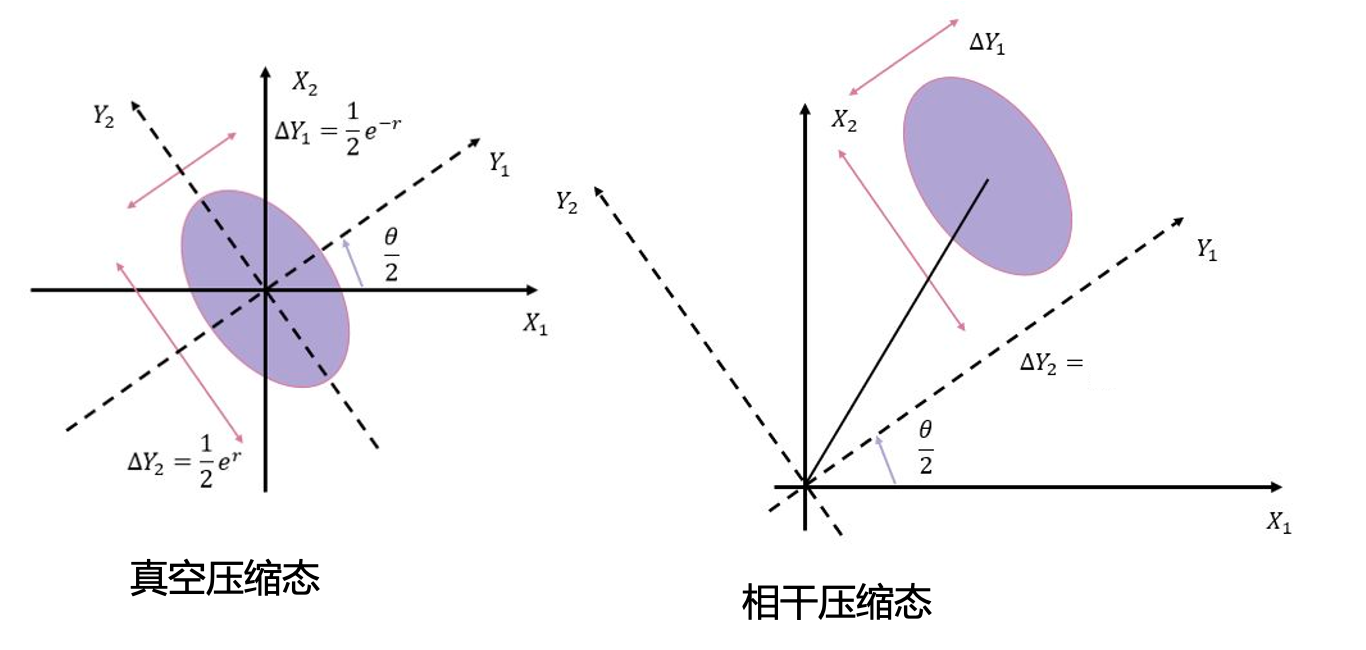
\includegraphics[width=1.0\textwidth]{figs/2022-05-02-13-13-46.png}
   \end{center}   
\end{frame}

\begin{frame}
    \frametitle{}
    压缩态相图
      \begin{center}
           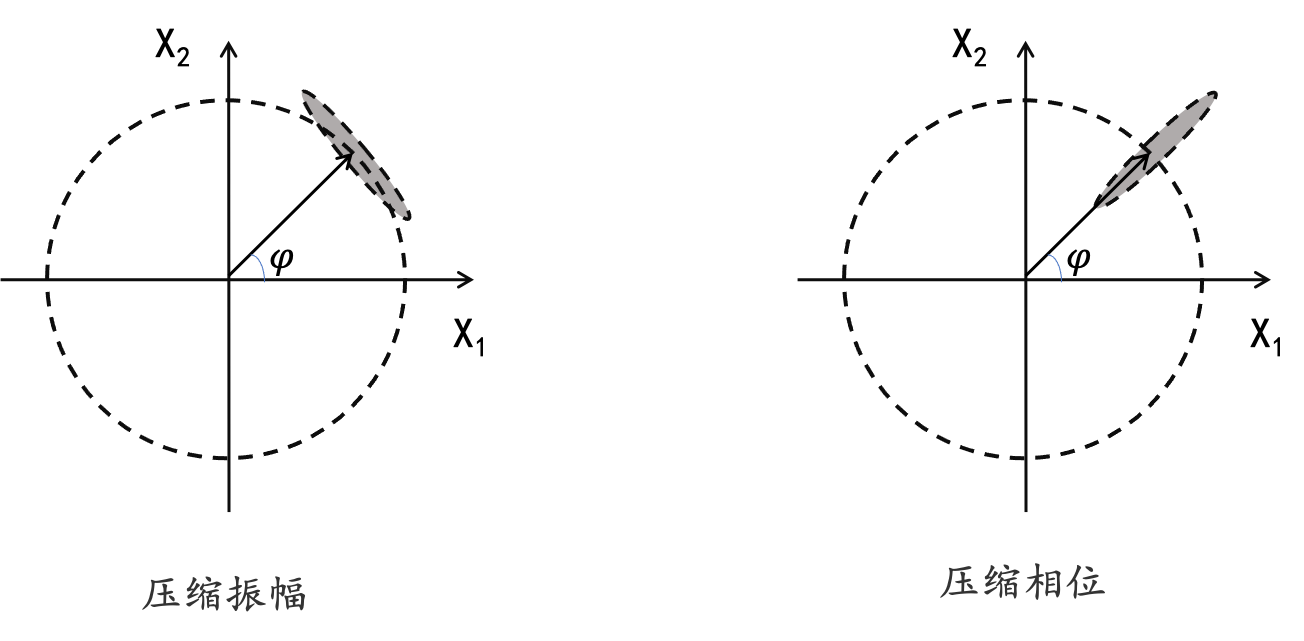
\includegraphics[width=1.0\textwidth]{figs/9.png}
      \end{center}   
   \end{frame}

\begin{frame}
 \frametitle{}
      电场分量的量子涨落:
      \[ \overline{ (\Delta \mathbf{E}(\mathbf{r},t))^2} = \frac{1}{L^3} (\frac{2\hbar \omega}{\varepsilon_0}) [ \overline{ (\Delta X_1)^2} \sin ^2 (\omega t - \mathbf{k}\cdot \mathbf{r}) + \overline{ (\Delta X_2)^2} \cos ^2 (\omega t - \mathbf{k}\cdot \mathbf{r}) ]\]
\end{frame}

   \begin{frame}
    \frametitle{}
    压缩态波形图
      \begin{center}
           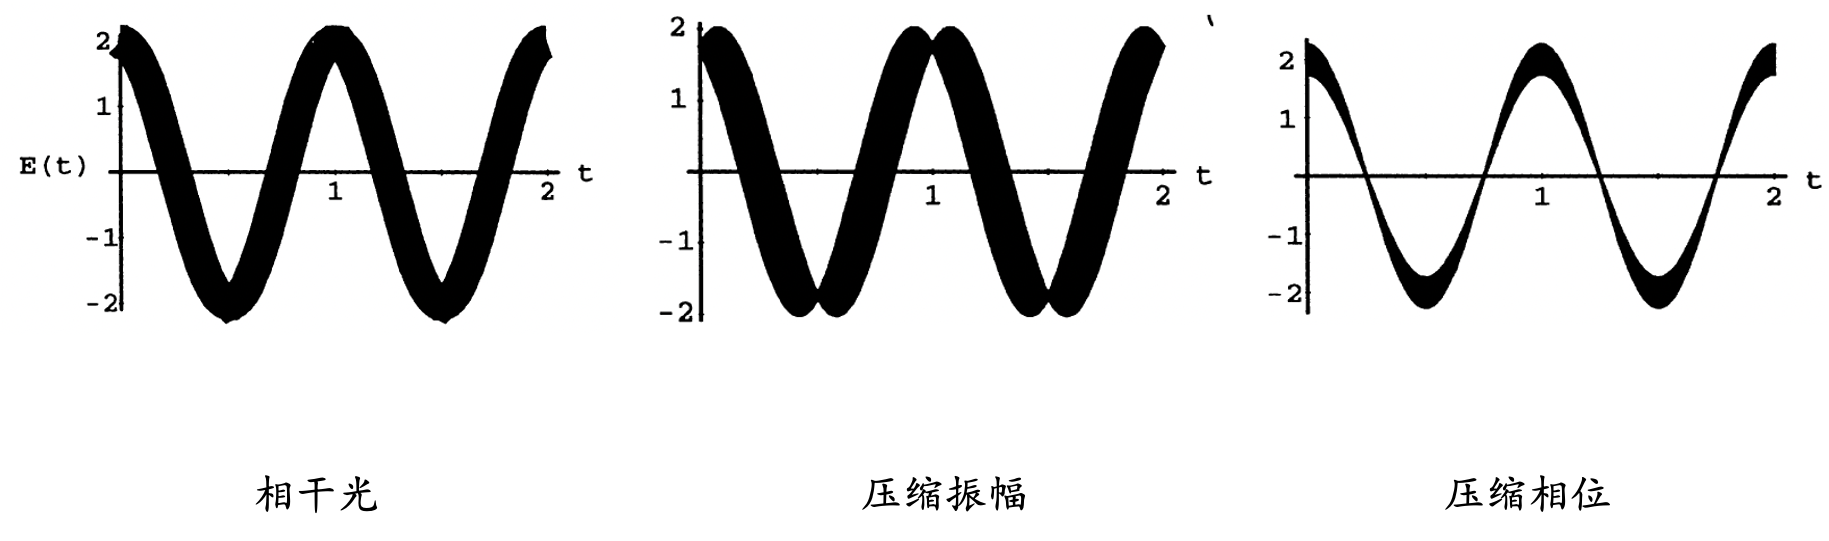
\includegraphics[width=1.0\textwidth]{figs/12.png}
      \end{center}   
   \end{frame}

\begin{frame}
    \例 [7.  求压缩态光子数的均值和涨落]{
    }
     \解~ 先计算均值: 
      \[ \begin{aligned}
        \overline{n} & = \left\langle a^{\dagger} a\right\rangle  \\ 
        &= \lcr{\xi} {a^{\dagger} a} {\xi} \\ 
        &= \lcr{\xi} {|\alpha|^{2}\left(\mu^{2}+|\nu|^{2}\right)-\alpha^{* 2} \mu \nu-\alpha^{2} \mu \nu^{*}+|\nu|^{2}} {\xi} \\ 
        &= (\mu \alpha^* _{+} - \nu^* \alpha _{+})(\mu \alpha _{+} - \nu \alpha ^* _{+}) + \left| \nu ^2 \right| \\ 
        &= \left|\alpha^2\right| + \left| \nu ^2 \right| \\ 
        &= \left|\alpha^2\right| + \sinh ^2 (r)
       \end{aligned}\]  
       如果是真空压缩态, $\alpha=0 $, 光子数均值为 $\sinh ^2 (r)$  
   \end{frame}

   \begin{frame}
    \frametitle{}
    \[ \begin{aligned}
        \overline{n^2} & = \left\langle (a^{\dagger} a)^2\right\rangle  \\ 
        &= \lcr{\xi} {a^{\dagger} a a^{\dagger} a} {\xi} \\ 
        &= \lcr{\xi} {a^{\dagger} (a a^{\dagger}) a} {\xi} \\ 
        &= \lcr{\xi} {a^{\dagger} (a^{\dagger} a +1) a} {\xi} \\ 
        &= \lcr{\xi} {a^{\dagger 2 }  a ^2 + a^{\dagger }a} {\xi} \\ 
        &= \lcr{\xi} {a^{\dagger 2 }  a ^2 } {\xi} +  \lcr{\xi} { a^{\dagger} a} {\xi} \\ 
        &= \overline{a^{\dagger 2 }  a ^2 } + \overline{n}
       \end{aligned}\] 
       式中,双光子项为 
       \[  \overline{a^{\dagger 2 }  a ^2 } = \left| \alpha ^4 \right| + \mu ^2 \left|\nu^2\right| - \mu (\alpha^2 \nu^* +cc) + 4 \left|\alpha^2 \right| \left|\nu^2\right| + 2 \left|\nu ^4\right|\] 
   \end{frame}

   \begin{frame}
    \frametitle{}
        粒子数涨落: 
    \[\begin{aligned}
             \Delta n & =\sqrt{ \overline{n^2} - (\overline{n})^2 } \\ 
             &= \sqrt{ \overline{a^{\dagger 2 }  a ^2 } + \overline{n} - (\overline{n})^2 }
    \end{aligned} \]
        占据数分布: 
      \begin{center}
           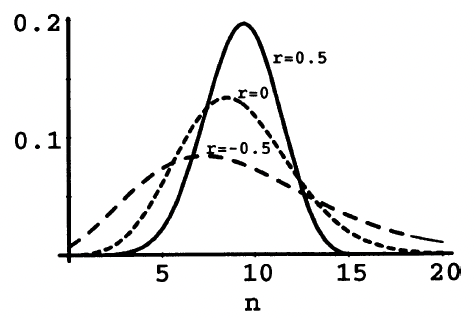
\includegraphics[width=0.5\textwidth]{figs/2022-05-03-23-54-35.png}
      \end{center}

   \end{frame}

   \begin{frame}
    \frametitle{压缩态随时间的演化} 
    \例 [7.  求压缩态随时间的演化规律]{
    }
    \解~ 增加时间演化因子, 场的正交分量为: 
    $$\left\{\begin{matrix}
        Y_1=\dfrac{1}{2}(a e^{-i (\omega t + \theta /2) }+a^\dagger e^{i (\omega t + \theta /2) })\\ 
        ~\\
        Y_2=\dfrac{1}{2i}(a e^{-i (\omega t + \theta /2) }-a^\dagger e^{i (\omega t + \theta /2) })
    \end{matrix}\right.$$
   \end{frame}

   \begin{frame}
    \frametitle{}
     对于压缩态,求均值, 可得: 
    \[ 
        \begin{aligned}
            &\left\langle Y_{1}(t)\right\rangle=\frac{1}{2} e^{-r}\left(\alpha e^{-i\left(\omega t+\frac{\theta}{2}\right)}+\alpha^{*} e^{i\left(\omega t+\frac{\theta}{2}\right)}\right) \\
            &\left\langle Y_{2}(t)\right\rangle=\frac{1}{2 i} e^{r}\left(\alpha e^{-i\left(\omega t+\frac{\theta}{2}\right)}-\alpha^{*} e^{i\left(\omega t+\frac{\theta}{2}\right)}\right) \\
            &\Delta Y_{1}(t)=\frac{1}{2} e^{-r} \\
            &\Delta Y_{2}(t)=\frac{1}{2} e^{r}
            \end{aligned} \]
    均值随时间谐振,即波包整体做简谐运动;场正交涨落值不变,波包形状不变  \\ 
   \end{frame}

   \begin{frame} 
   \frametitle{相图的变化}
   \begin{center}
    \animategraphics[height=2in,loop]{30}{gif/cohs-}{1}{100} 
    \end{center} 
   \end{frame}

   \begin{frame} 
    \frametitle{位置表象中的变化}
    \begin{center}
     \animategraphics[height=1.8in,loop]{30}{gif/vs-}{1}{120}   \animategraphics[height=1.8in,loop]{30}{gif/cohs1-}{1}{120}
     \end{center} 
    \end{frame}

   \section{4. 压缩态的产生}

   \begin{frame}
    \frametitle{压缩态的产生}
  理论上,应基于非线性效应,构造含双光子过程的系统, 具有如下压缩算符. 
  \[ S(\xi) = e^{\frac{1}{2}[\xi^* a^2 - \xi (a^{\dagger}) ^2]}\]

  \begin{itemize}
      \item  参量放大下转换
      \item  铁电原子系综三阶非线性效应 ~~ 四波混频
      \item  光纤的三阶非线性效应
      \item  二次谐波
      \item  共振荧光
  \end{itemize}

  \end{frame}
  
  \begin{frame}
        \frametitle{参量下转换}
  非线性介质具有多光子过程: \\ 
  介质中, 电位移矢量与场强和极化矢量有如下关系:
  \[ \mathbf{D}=\epsilon_0 \mathbf{E} + \mathbf{P}  \]
  通常, 可以认为 $\mathbf{P}$ 对 $\mathbf{E}$ 是线性的. 
  \[\mathbf{P}(\omega)= \epsilon_0 \chi(\omega) \mathbf{E}(\omega) \]
  实际上, 它的Taylor展开如下: (线性只是其一阶近似).
  \[ P_{i}=\varepsilon_{0}\left[\chi_{i j}^{(1)} E_{j}+\chi_{i j k}^{(2)} E_{j} E_{k}+\chi_{i j k l}^{(3)} E_{j} E_{k} E_{l}+\cdots\right] \]
  考虑二阶项, 对应材料吸收一种频率的光子,产生倍频成份新光子. 称为非线性介质的参量下转换. 
\end{frame}

\begin{frame}
 \frametitle{}
        \begin{center}
             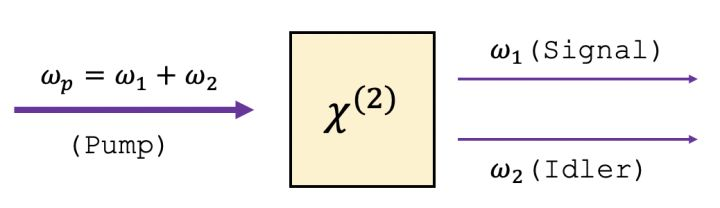
\includegraphics[width=0.7\textwidth]{figs/2022-05-02-20-00-04.png}
        \end{center}
        考虑简并参量放大 (OPA) $\omega_s = \omega_i = \omega = \frac{1}{2} \omega_p$, 这个过程的哈密顿 可写成: 
    \[ 
        \begin{aligned}
            H_{nl} & = \gamma  \Phi\left(k_{p} ; k_{1}, k_{2}\right) a_{k_{p}} ^ \dagger  a_{k_{1}} a_{k_{2}} - \gamma  \Phi\left(k_{p} ; k_{1}, k_{2}\right) a_{k_{p}} a_{k_{1}}^{\dagger} a_{k_{2}}^{\dagger} \\ 
            &= i \hbar \chi ^{(2)} (\omega_p, \omega) [ a^2 b^\dagger -  a ^{\dagger 2} b ]
            \end{aligned} \]
    其中, $a$和$b$分别不信号场($\omega$) 光子和泵浦场($\omega_p$)光子的湮灭算符.  \\ 
    当满足一定的相位匹配条件时, 信号波将被放大,并伴随有与信号波同频率的空闲波产生. 
\end{frame}

\begin{frame}
 \frametitle{}
     通常泵浦源为激光, 是相干态, 带上时间, 有:
    \[ b(t) = \beta e ^{-i \omega_p t} = \beta e ^{-i 2 \omega t} \]
    信号波与空闲波同频,有:
     \[ H_{nl} = i \frac{\hbar}{2} \chi [ a^2 e ^{i 2 \omega t} -  a ^{\dagger 2} e ^{-i 2 \omega t}]  \]
     时间演化算符正好具有压缩算符的形式: 
     \[U(\xi, t) = e^{- i \frac{H_{nl}}{\hbar} t}  =  e^{\frac{1}{2}[\xi^* a^2 - \xi a^{\dagger 2} ]} \]
    对比定义, 可确定各参数.
    \[ \xi = r e ^ {i \theta } \]
\end{frame}

\begin{frame}
      \frametitle{}
      
现加上一阶项, 得总哈密顿: 
     \[ 
       \begin{aligned}
           H & = H_l + H_{nl} \\ 
           &= \hbar \omega a ^{\dagger } a  + \frac{1}{2}\hbar \omega  - i \frac{\hbar}{2} \chi [ a^2 e ^{i 2 \omega t} -  a ^{\dagger 2} e ^{-i 2 \omega t}]  \cdots  (1) 
           \end{aligned} \]

 取相互作用绘景: 
 \[ a_I(t) = a(t) e ^{i \omega t},  \qquad a^\dagger _I(t) = a^\dagger (t) e ^{-i \omega t} \cdots  (2)\] 
 把(1)(2)代入海森堡方程, 有: 
 \[ 
    \begin{aligned}
        \frac{\mathrm{d}a_I(t)}{\mathrm{d}t} & = \frac{1}{i \hbar} [a_I(t), H ] = \chi a^\dagger _I(t)  \\ 
        \frac{\mathrm{d}a^\dagger _I(t)}{\mathrm{d}t} & = \frac{1}{i \hbar} [a^\dagger _I(t), H ] = \chi a_I(t)  \\
    \end{aligned} \]
    解得: 
    \[ a_I(t) = a_I(0) \cosh(\chi t )e^{-\omega t} - i \frac{\alpha_0}{\left|\alpha_0\right|} a^\dagger_I(0) \sinh(\chi t ) e^{\omega t}\]
\end{frame}   

\begin{frame}
 \frametitle{}
 根据  \[ \hat{X}_{1} =\frac{1}{2}\left(a + a^{\dagger}\right)\]
 \[ \hat{X}_{2} = \frac{1}{2 i}\left(a - a^{\dagger}\right)\]
写出相互作用绘景下的场方程: 
\[ \frac{\mathrm{d}X_1}{\mathrm{d}t} =  \chi X_1 , \qquad  \frac{\mathrm{d}X_2}{\mathrm{d}t} = - \chi X_2  \]
解得: 
\[ X_1(t) = X_1 (0) e ^{\chi t}\]
\[ X_2(t) = X_2 (0) e ^{-\chi t}\]
\end{frame}

\begin{frame}
 \frametitle{}
    量子涨落(均方差): 
    \[\overline{(\Delta X_1(t))^2} = \overline{(\Delta X_1(0))^2}  e^{2\chi t}  \]
    \[\overline{(\Delta X_2(t))^2} = \overline{(\Delta X_2(0))^2}  e^{-2\chi t}  \]
    经典条件下, 除了泵浦激光源, 还必须提供信息光. \\ 
    量子条件下,无需信息光,可以直接从真空态激发, 称为自发参量下转换. 
    \[ \rs{\beta} \rs{0}_s  \rs{0}_i \to \rs{\beta} \rs{1}_s  \rs{1}_i \]
    取$t=0$, 处于真空态(相干态), 有:
    \[\overline{(\Delta X_1(0))^2} = \overline{(\Delta X_2(0))^2} =\frac{1}{4}\]
    当$t>0$, 场分量$X_2$被有效压缩, 压缩的程度与三个因素有关: (1) 二阶非线性极化系数$\chi^{(2)}$, (2) 泵浦激光源强度 $\beta$,  (3) 时间 $t$ 
\end{frame}

\begin{frame}
    \frametitle{}
    \begin{center}
        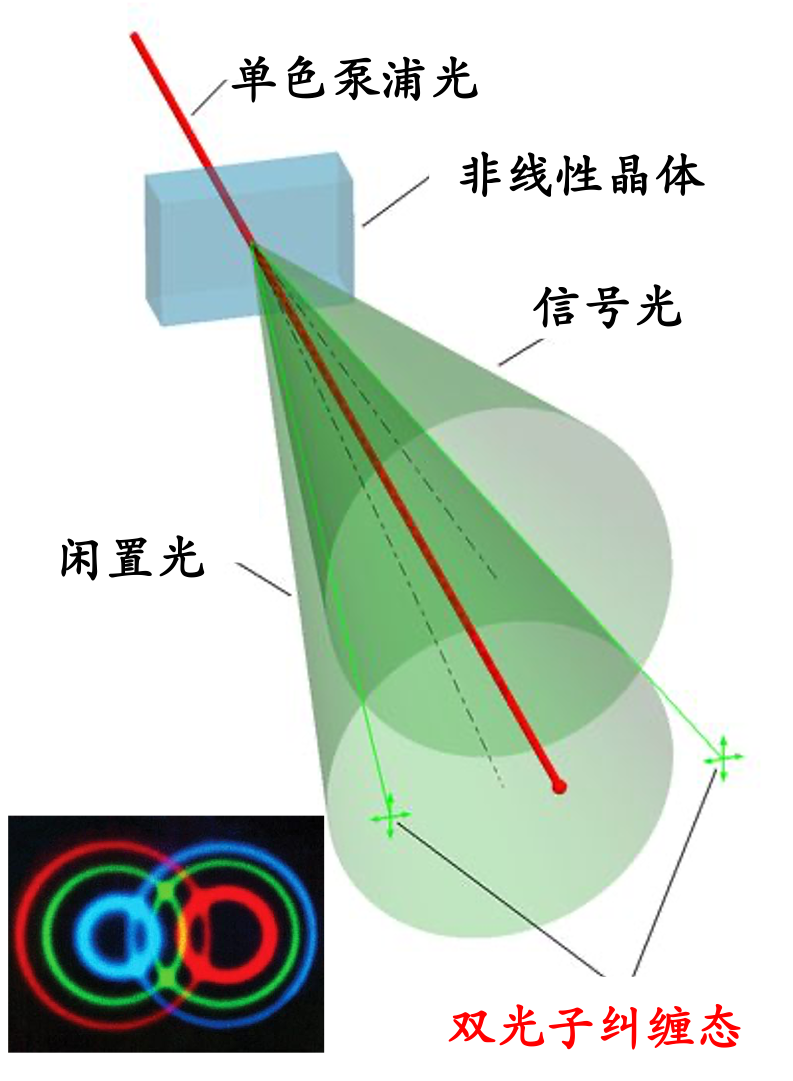
\includegraphics[width=0.29\textwidth]{figs/32.png}
    \end{center} 
    应用:
 \begin{enumerate}
     \item 单光子源 : 测得闲置光子,则必有信号光子! 由于产生光子对的概率很低, 同一时刻产生两个信号光子的概率趋零. 因此是单光子源。
     \item 纠缠光子双: 闲置光子与信号光子同时产生, 存在多个自由度的纠缠
 \end{enumerate} 
\end{frame}

\section{5. 双光子纠缠态}

\begin{frame} 
    \frametitle{量子纠缠的定义}
    {\Bullet} ~双量子比特是单量子比特的张量积,因此可写成四个计算基矢的叠加态:
    \[\rs{\psi} =(a_0\rs{0}+a_1\rs{1})\otimes (b_0\rs{0}+b_1\rs{1})=\alpha_{00}\rs{00}+\alpha_{01}\rs{01}+\alpha_{10}\rs{10}+\alpha_{11}\rs{11}\]
    {\Bullet} 定义:如果双量子比特的态函数不能写在单量子比特函数的张量积,则称它们所处的状态为量子纠缠态
    \[\rs{\psi} \neq \rs{\psi_{1}} \otimes \rs{\psi_{2}} \]
\end{frame} 

\begin{frame} 
    \frametitle{}
    \例 [8. 试确定下列态哪些是纠缠态]{}
    {\[ \Psi_1=\frac{\rs{00}+\rs{11}}{\sqrt{2}}; \qquad \Psi_2=\frac{\rs{01}+\rs{10}}{\sqrt{2}} ; \qquad \Psi_3=\frac{\rs{00}+\rs{10}}{\sqrt{2}} \]}
    \解~ $\Psi_3$不是纠缠态
    \[\begin{aligned}
        \Psi_3 &= \frac{\rs{00}+\rs{10}}{\sqrt{2}} \\
        &= \frac{\rs{0}+\rs{1}}{\sqrt{2}}\otimes \rs{0} \\
        &= \frac{\rs{0}+\rs{1}}{\sqrt{2}}\otimes (\rs{0}+0\rs{1}) \\
        &= \rs{\psi_{1}} \otimes \rs{\psi_{2}} 
    \end{aligned}\] 
\end{frame} 

\begin{frame}
    \frametitle{量子擦除实验}
    光子对的制备:激光与非线性光学介质发生作用时,产生多种非线性光学效应,比如:自发参量下转换(SPDC): 
    \begin{center}
        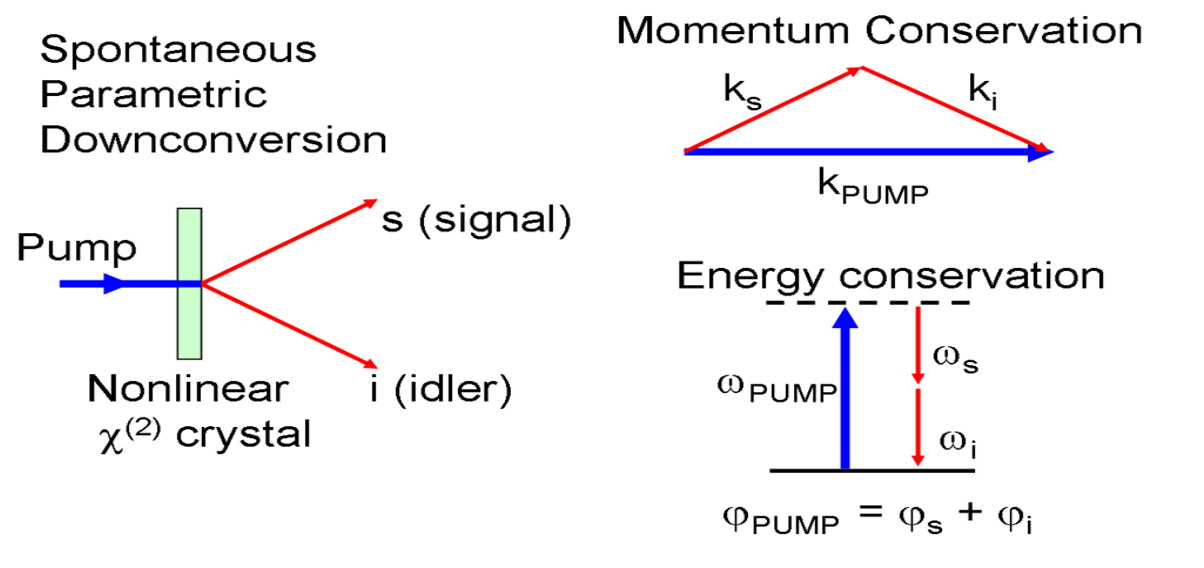
\includegraphics[width=0.7\textwidth]{figs/31a.png}
    \end{center}
    每一个光子在被非线性晶体散射时,以一定概率转化为频率相同波矢不同的光子对(信号光子和闲置光子),是纠缠光子对。
\end{frame}

\begin{frame}
    \frametitle{量子擦除实验}
    \begin{center}
        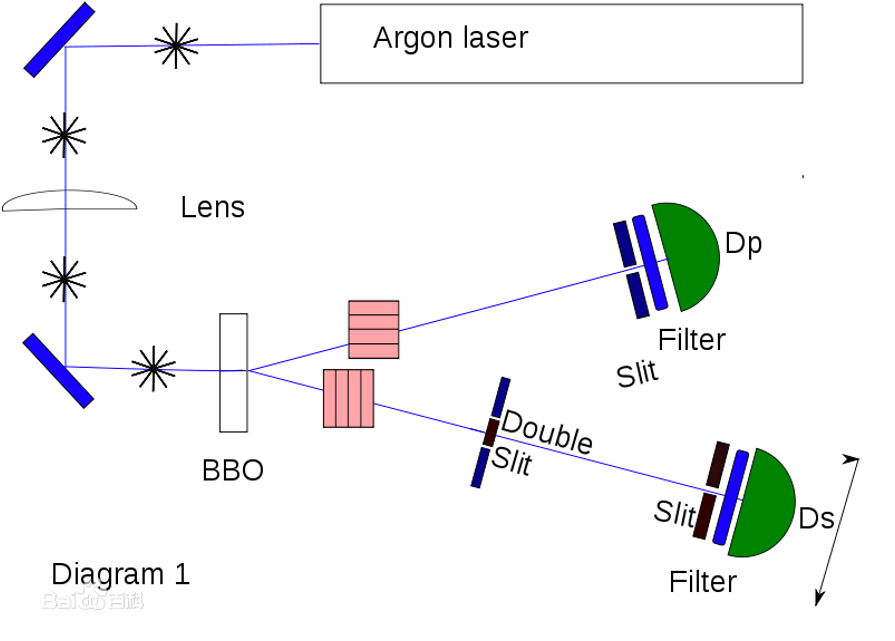
\includegraphics[width=0.55\textwidth]{figs/c1.png}
    \end{center}
    BBO晶体产生光子对,下路径光子过双缝形成干涉条纹.
\end{frame} 

\begin{frame}
    \frametitle{}
    \begin{center}
        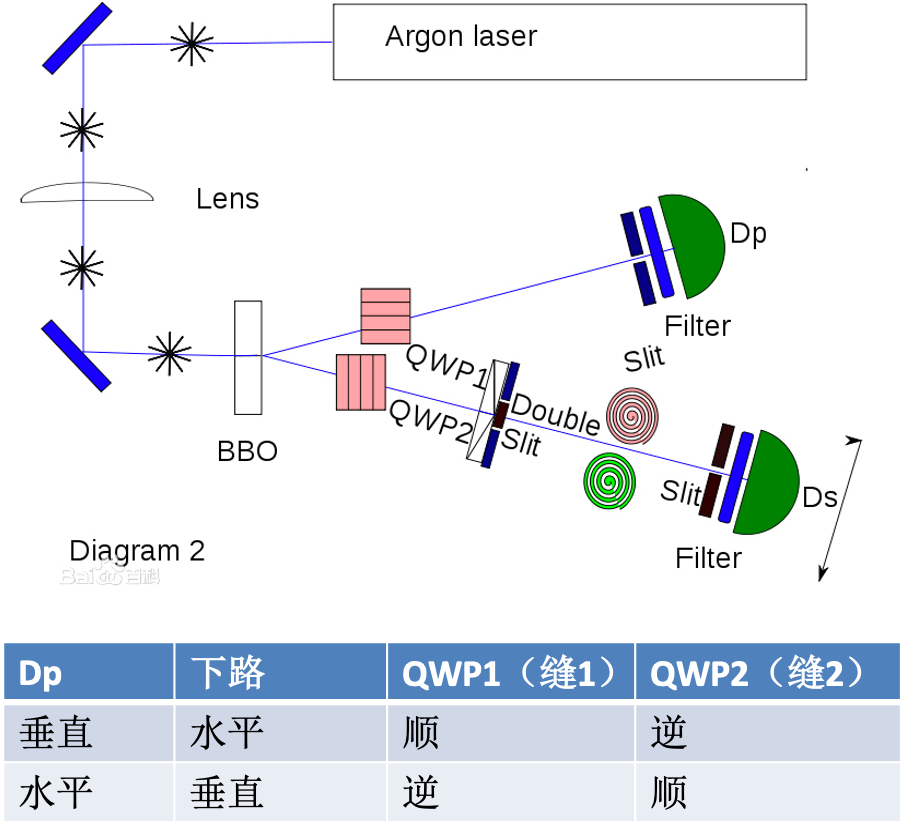
\includegraphics[width=0.6\textwidth]{figs/c2.png}
    \end{center}
    插入四分之一波片(QWP)进行路径测试,干涉条纹消失
\end{frame} 

\begin{frame}
    \frametitle{}
    \begin{center}
        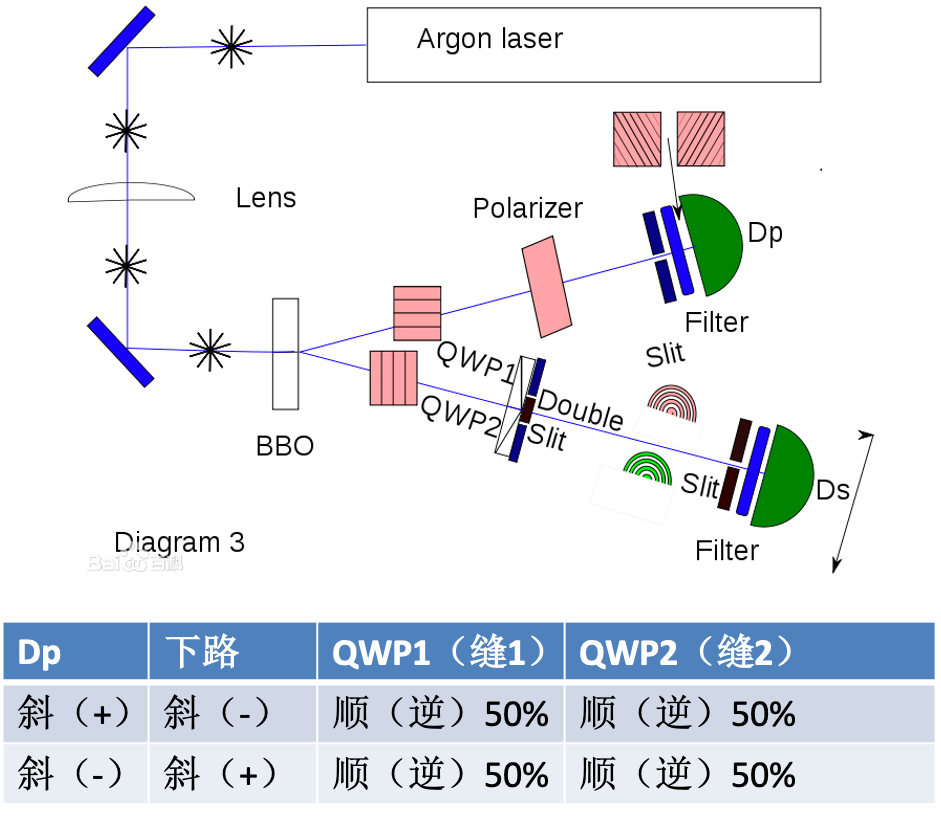
\includegraphics[width=0.6\textwidth]{figs/c3.png}
    \end{center}
    上光路径插入起偏器(Polarizer)下光路干涉条纹重新出现!
\end{frame} 

\begin{frame}
    问题: 起偏器改变的是上光子的偏振,为什么下光路干涉条纹重新出现?\\ \vspace{0.8em}
    结论: 自发参量下转换产生的是纠缠光子对,存在超距离相互作用
\end{frame} 

\begin{frame} 
    \frametitle{~EPR态}
    \begin{center}
        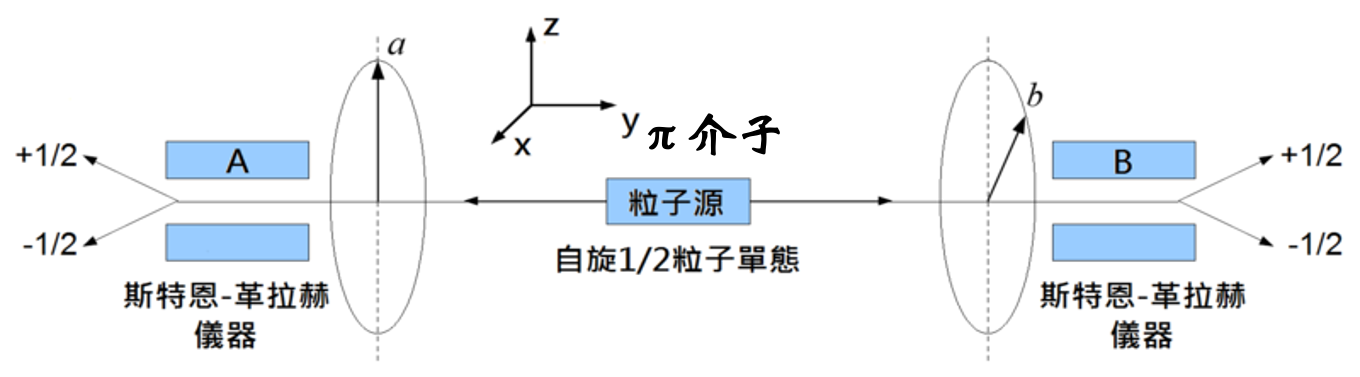
\includegraphics[width=0.78\textwidth]{figs/28a.png}
    \end{center}
    {\Bullet} 是否存在超距离相互作用?\\
    {\Bullet} 电子EPR态是纠缠态\[\rs{EPR}=\frac{\rs{\uparrow \downarrow }-\rs{\uparrow \downarrow }}{\sqrt{2}} = \frac{\rs{01 }-\rs{10 }}{\sqrt{2}} \]
    {\Bullet} 光子EPR态也是纠缠态\[\rs{EPR}=\frac{\rs{\leftarrow \rightarrow }-\rs{\rightarrow \leftarrow }}{\sqrt{2}} = \frac{\rs{01 }-\rs{10 }}{\sqrt{2}} \]
\end{frame} 

\begin{frame}
    \frametitle{贝尔(Bell)不等式}
    \begin{center}
        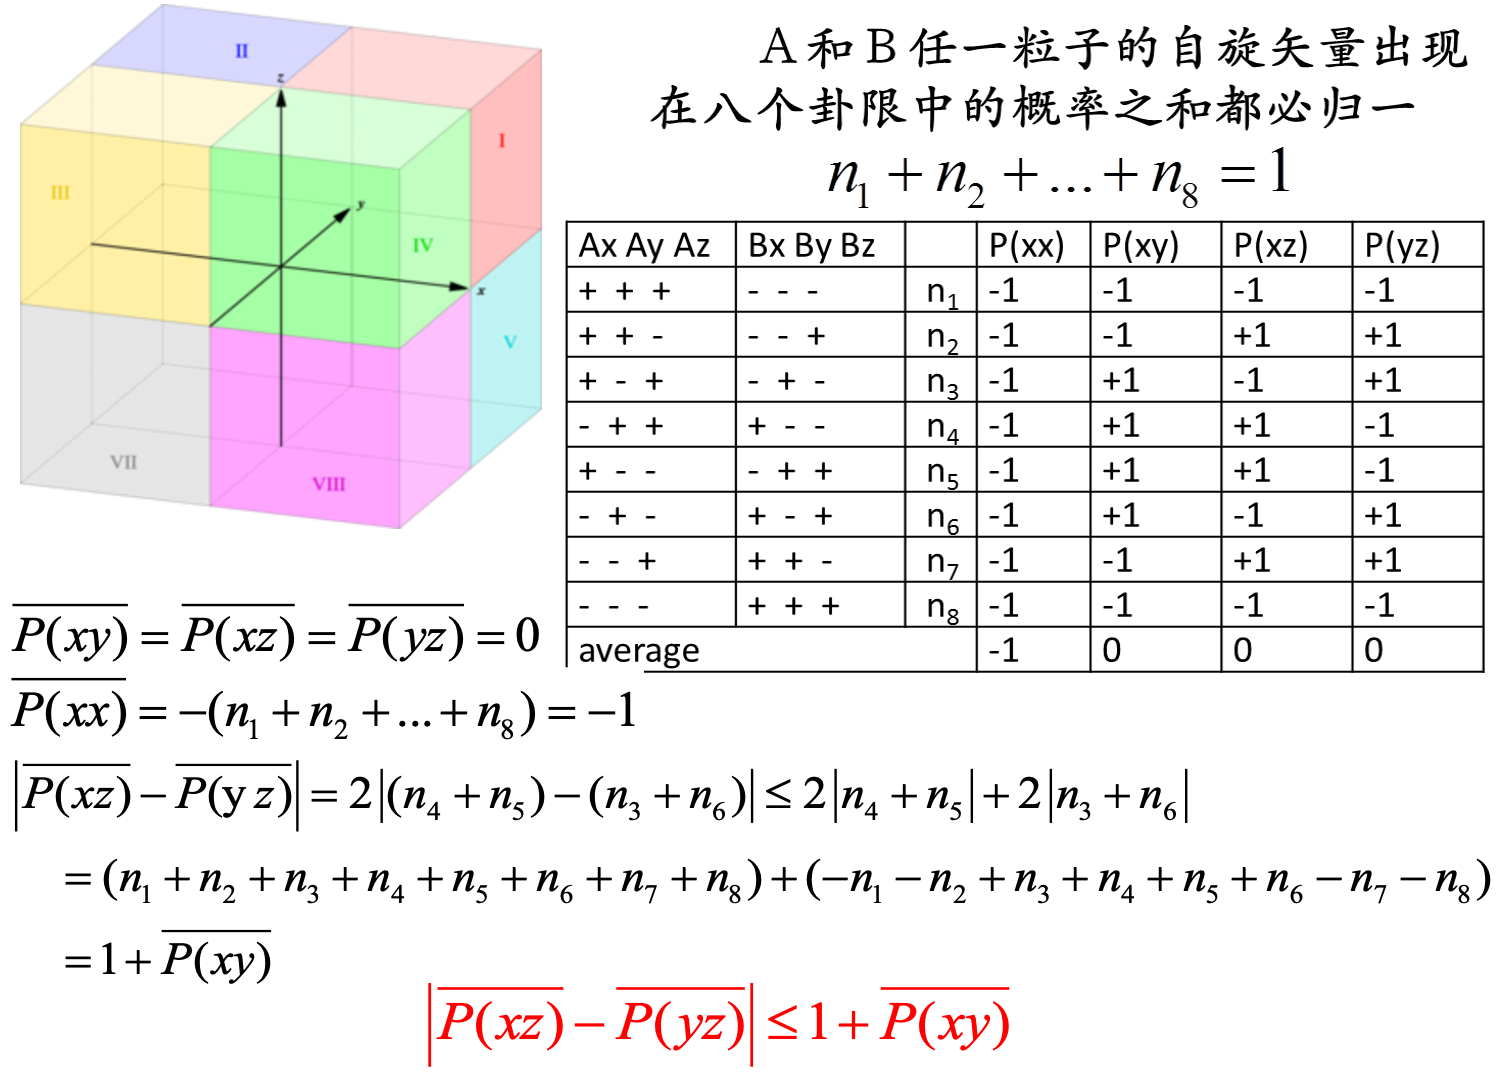
\includegraphics[width=0.75\textwidth]{figs/29a.png}
    \end{center}
\end{frame} 

\begin{frame} 
    \frametitle{贝尔态}
    \[\rs{\beta_{00}}=\frac{\rs{00}+\rs{11}}{\sqrt{2}} =\frac{1}{\sqrt{2}} \begin{bmatrix}
        1 \\
        0 \\
        0 \\
        1
     \end{bmatrix} ; \qquad \rs{\beta_{01}}=\frac{\rs{00}-\rs{11}}{\sqrt{2}} = \frac{1}{\sqrt{2}} \begin{bmatrix}
        1 \\
        0 \\
        0 \\
        -1
     \end{bmatrix} \]
    \[\rs{\beta_{10}}=\frac{\rs{01}+\rs{10}}{\sqrt{2}} =\frac{1}{\sqrt{2}} \begin{bmatrix}
        0 \\
        1 \\
        1 \\
        0
     \end{bmatrix} ; \qquad \rs{\beta_{11}}=\frac{\rs{01}-\rs{10}}{\sqrt{2}} =\frac{1}{\sqrt{2}} \begin{bmatrix}
        0 \\
        1 \\
        -1 \\
        0
     \end{bmatrix} \]
\end{frame}

\begin{frame}
    \frametitle{}
    \例 [9. 试证明贝尔态构成正交归一完备集]{}
    \证~归一性 \[\begin{aligned}
        \lr{\beta_{00}}{\beta_{00}} &= \frac{(\ls{00}+\ls{11})(\rs{00}+\rs{11})}{2} \\
        &= \frac{\lr{00}{00}+\lr{00}{11}+\lr{11}{00}+\lr{11}{11}}{2} \\
        &= \frac{1+0+0+1}{2} = 1 
    \end{aligned}\]
    正交性 \[\begin{aligned}
        \lr{\beta_{00}}{\beta_{01}} &= \frac{(\ls{00}+\ls{11})(\rs{00}-\rs{11})}{2} \\
        &= \frac{\lr{00}{00}+\lr{00}{11}+\lr{11}{00}-\lr{11}{11}}{2} \\
        &= \frac{1+0+0-1}{2} = 0 
    \end{aligned}\]
\end{frame}

\begin{frame}
    \frametitle{}
    \例 [10. 试证明贝尔态是纠缠态]{}
    \证~反正法,有单态
    \[ \rs{a} = a_0\rs{0}+a_1\rs{1}; \qquad \rs{b} = b_0\rs{0}+b_1\rs{1}\]
    设贝尔态可以写成单态的张量积
    \[ \begin{aligned}
    \beta_{00} &= \rs{a}\otimes \rs{b} \\
    \frac{\rs{01}+\rs{10}}{\sqrt{2}} &= (a_0\rs{0}+a_1\rs{1}) \otimes (b_0\rs{0}+b_1\rs{1}) \\
    &= a_0b_0\rs{00}+ a_0b_1\rs{01}+a_1b_0\rs{10}+a_1b_1\rs{11}
    \end{aligned}\]
    上式要成立,要求$a_0b_1\ne 0, a_1b_0 \ne 0; \quad \to \quad a_0b_1a_1b_0\ne 0$ \\
    上式要成立,要求$a_0b_0= 0, a_1b_1 = 0; \quad \to \quad a_0b_1a_1b_0= 0$ \\
    自相矛盾,证毕!
\end{frame}

\section{6. 压缩态的探测}

\begin{frame}
    \frametitle{平衡零差探测}
           \begin{center}
                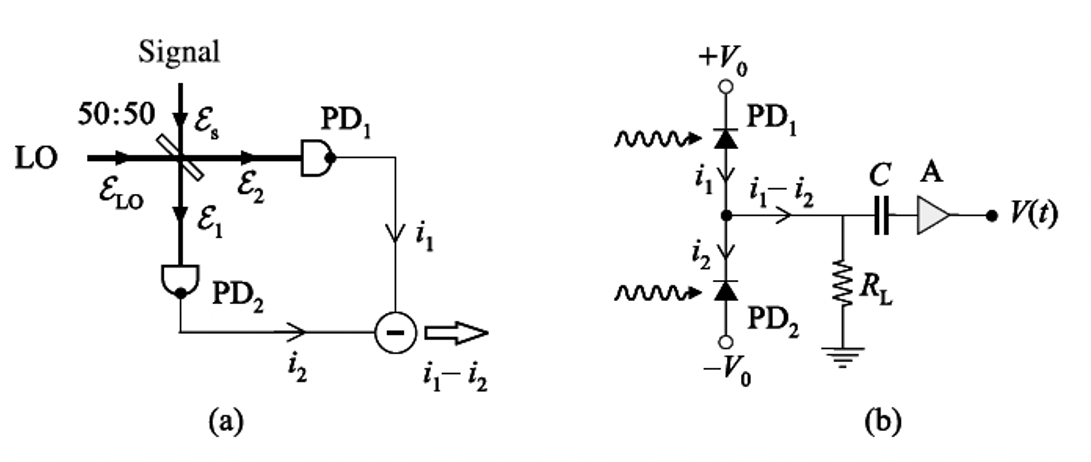
\includegraphics[width=0.8\textwidth]{figs/14.png}
           \end{center}
       基于一个平衡分束器(50:50)和两个光电二极管(PD)的平衡零差探测器实验装置图. ~~  
       LO: 本地振荡器, A: 放大器. 本地振荡器发出探测光场, 把信号光场(Signal)的信息带入输出电压V(t)中,从而实现对信号光场的探测.  
   \end{frame}
   
   
   \begin{frame}
       \frametitle{}~
       {\Bullet}信号分析: {\vspace*{0.3em}}
       零差意指两光场同频(中心频率~$\omega$~), 因此, 这是两光场相干问题. \\ 探测光场是强场 (经典处理) , 信号光场是弱场(量子化), 设两光场的相位差为$\phi$, 
       \[ E_L e^{i\phi} = E_L(\cos\phi + \sin\phi)\]
       \[ E_s  =  E_s ^{X_1}  + i E_s ^{X_2}\]
       注意到半波损失,输入输出关系为:
       \[ E_1  =  \frac{1}{\sqrt{2}} (E_L e^{i\phi} + E_s) = \frac{1}{\sqrt{2}} [ (E_L\cos\phi + E_s ^{X_1} ) + i (E_L\sin\phi + E_s ^{X_2} ) ]\]
       \[ E_2  =  \frac{1}{\sqrt{2}} (E_L e^{i\phi} - E_s) = \frac{1}{\sqrt{2}} [ (E_L\cos\phi - E_s ^{X_1} ) + i (E_L\sin\phi - E_s ^{X_2} ) ] \] 
      \end{frame}
   
      \begin{frame}
       \frametitle{}
       \[ \begin{aligned}
           V(t) &\propto  i_1 - i_2 \\ 
           &\propto  E_1 E^* _1 - E_2 E^* _2  \\ 
           &= 2 E_L ( \cos \phi E_s ^{X_1} + \sin \phi E_s ^{X_2} )
       \end{aligned} \]
       增加移相器\\  
       (1)  $\phi= 0, \pi, 2\pi, \cdots $, 可测得信号光场的$X_1$
       \[ V_1 \propto 2 E_L E_s ^{X_1} \]
       (2)  $\phi= \frac{\pi}{2}, \frac{3\pi}{2}, \cdots $, 可测得信号光场的$X_2$
       \[ V_2 \propto 2 E_L E_s ^{X_2} \]
       因此, 平衡零差探测可用来测量压缩态
      \end{frame}
   
      \begin{frame}
       \frametitle{}
       {\Bullet}噪声分析: \\ 
       如果没有信号光场的输入, 则相当于是真空场的输入, 噪声正是与探测光场同频的真空态的正交分量. 称为散粒噪声(shot-noise)  
   \end{frame}
   
   \begin{frame}
         \frametitle{}
         ~~\\ 
       {\Bullet}真空压缩态测量 \\ 
       如果是真空态被压缩, 则  $ V_1 \not= V_2$, 因此, 平衡零差探测可用来测量真空压缩态
         \begin{center}
              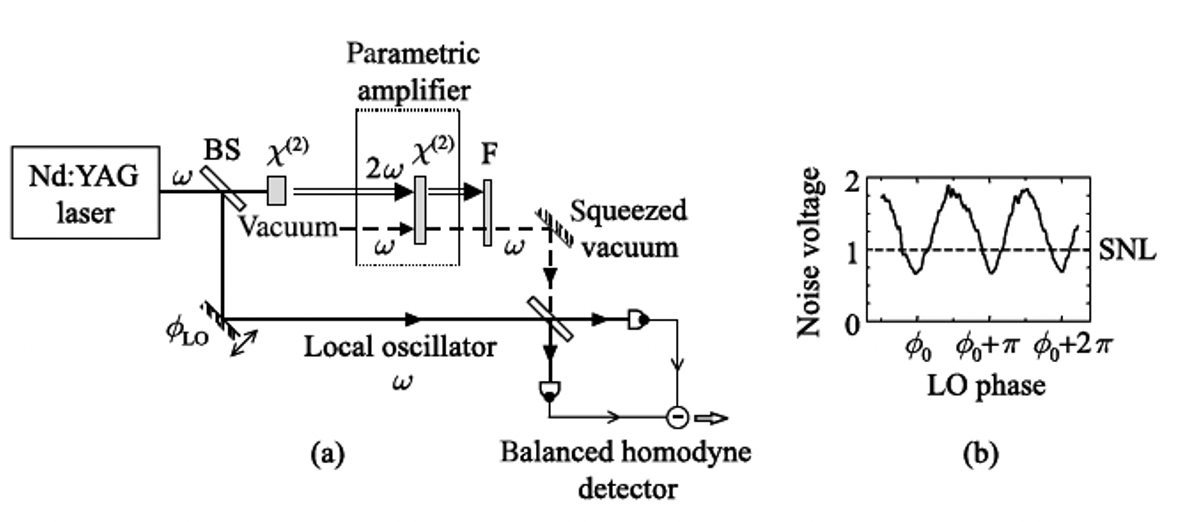
\includegraphics[width=0.9\textwidth]{figs/15.png}
         \end{center}
      \end{frame}    % 压缩态
%

\begin{frame}
    \frametitle{前情回顾}
    \begin{itemize}
        \item 量子化光场~~真空态~~产生湮灭算符 
        \item 相干态~~ 平移算符 ~~相图
        \item 压缩态~~ 压缩算符
        \item 数态表象~~数态展开
        \item 参量下转换~~平衡零差探测 
    \end{itemize}     
\end{frame}

%%%%%%%%%%%%%%%%%%%%%%%%%%%%%%%%%%
\begin{frame} [plain]
    \frametitle{}
    \Background[1] 
    \begin{center}
    {\huge 第10-11讲:光子统计}
    \end{center}  
    \addtocounter{framenumber}{-1}   
\end{frame}
%%%%%%%%%%%%%%%%%%%%%%%%%%%%%%%%%%

\section{1. 光子计数}

\begin{frame}
 \frametitle{计数技术概要}
    {\Bullet} 盖革-米勒计数器
    \begin{center}
        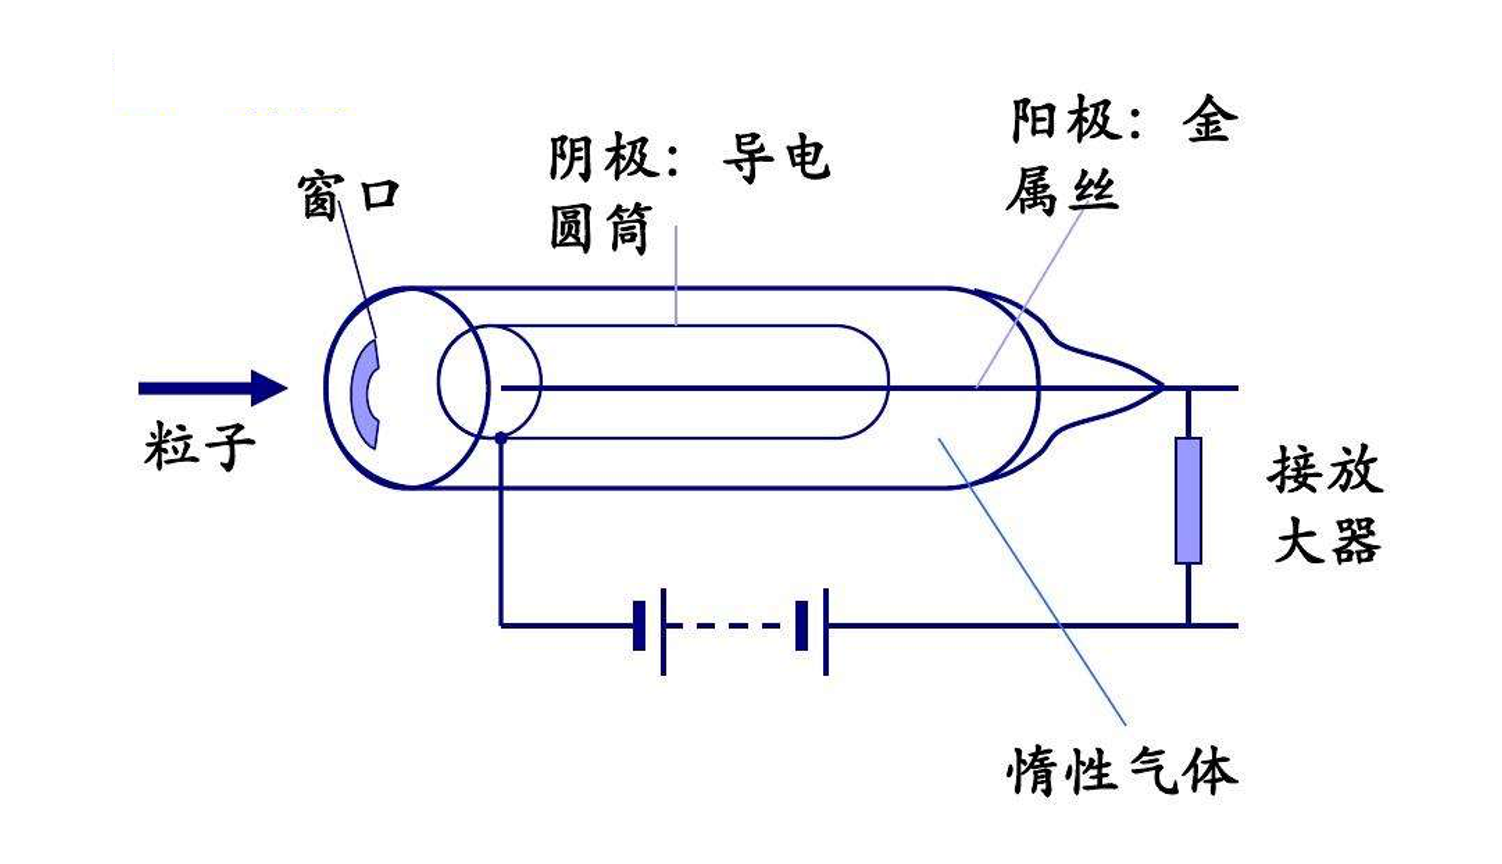
\includegraphics[width=0.7\textwidth]{figs/16.png}
    \end{center}  
\end{frame}

\begin{frame}
 \frametitle{}
 工作原理: 设备初始电压略低于管内稀薄气体击穿电压的, 一个带电粒子射入气体, 原子受激发射紫外光子, 光子射到阴极产生光电子, 光电子向阳极漂移,电离沿途气体,引起离子增殖, 形成自激放电. 输出一个脉冲电流信号.\\  {\vspace*{0.6em}}
      特点: 非常灵敏, 造价低廉、使用方便、探测范围 \\ 
      缺点: 不适合极快速计数, 不能区别粒子类型 \\ 
      著名成果: \\ 
      \begin{enumerate}
          \item 1911年, 卢瑟福用来计数$\alpha$粒子, 提出有核原子模型
          \item 1937年, 测定了宇宙射线的角分布
          \item 目前依然是核物理学和粒子物理学中不可缺少的探测器 
      \end{enumerate}
\end{frame}

\begin{frame}
 \frametitle{}
    {\Bullet} 单光子计数\\  {\vspace*{0.6em}}
    光子流量 ($\varPhi $): 单位时间通过的光子数 \\  光流强度 (P): 单位时间通过的光的能量 \\ 
    对于单色光(频率$\omega $), 有关系式:
    $$ ~~P = \varPhi  \cdot \hbar \omega  $$ \\ 
    当P降低到$10^{-16} W $时, 称为弱光, 可见光子流量约为 ~1~ ms 每光子, 必须考虑单光子计数
\end{frame}

\begin{frame}
      \frametitle{}
      {\Bullet} 真空光电倍增管\\ 
      \begin{center}
           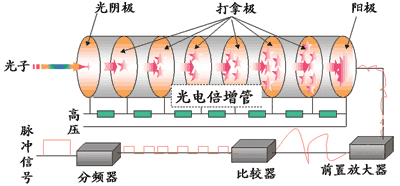
\includegraphics[width=0.6\textwidth]{figs/2022-05-04-16-57-37.png}
      \end{center}
      工作原理: 单光子在光阴极打出一个光电子, 光电子打在第一倍增极并被拿住, 第一倍增极发出数倍的二次电子, ...经数十级打拿增殖, 在阳极回路输出一个脉冲电流信号.  \\ {\vspace*{0.6em}}
    信噪比: (1) 光场的统计涨落, (2) 光阴极热电子, (3) 脉冲堆积效应
\end{frame}

\begin{frame}
 \frametitle{}
    {\Bullet} 雪崩光电二极管\\  {\vspace*{0.6em}}
      \begin{center}
           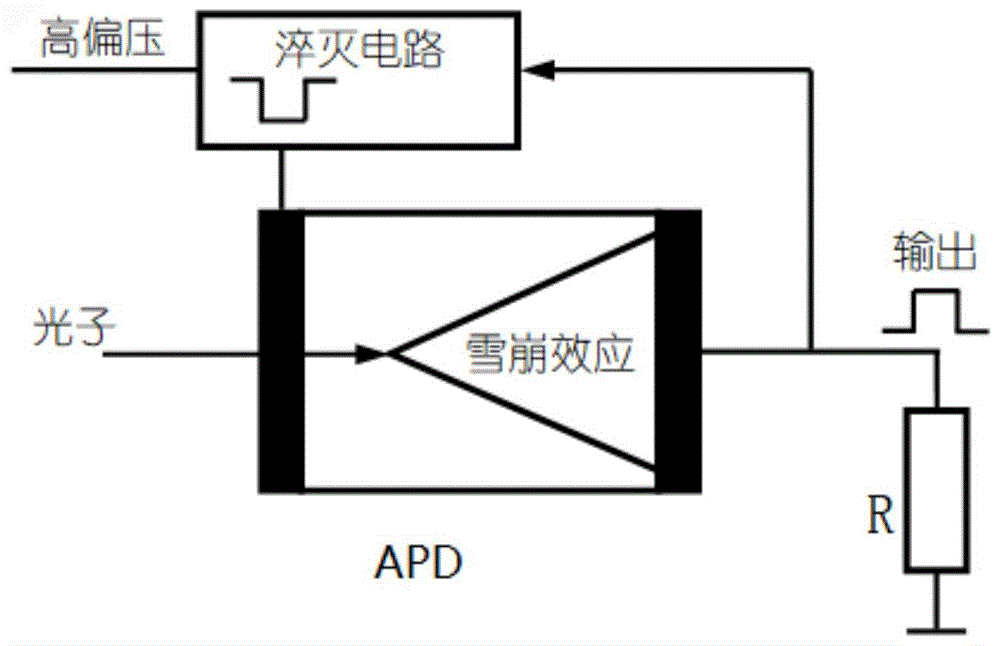
\includegraphics[width=0.45\textwidth]{figs/2022-05-04-18-25-01.png}
      \end{center}

    工作原理: PN 结工作在反向击穿电压附近, 吸收光子时, 光生载流子在强电场下运动,沿途原子电离实现载流子雪崩式增殖, 产生击穿脉冲电流信号.  \\  {\vspace*{0.6em}}

    特点: 在一个探测周期内最多只能完成一次计数. \\ 
    信噪比: (1) 光场的统计涨落, (2) 热生载流子, (3) 脉冲堆积效应 
\end{frame}

\begin{frame}
 \frametitle{}
 {\Bullet} 光场统计分布对计数的影响\\ 
 \begin{enumerate}
     \item 漏掉光子(没有脉冲)
     \item 漏掉计数(没有脉冲峰重叠)
     \item 每次计数窗口的计数不同,波动大.
     \item ...
 \end{enumerate} 
 \begin{center}
      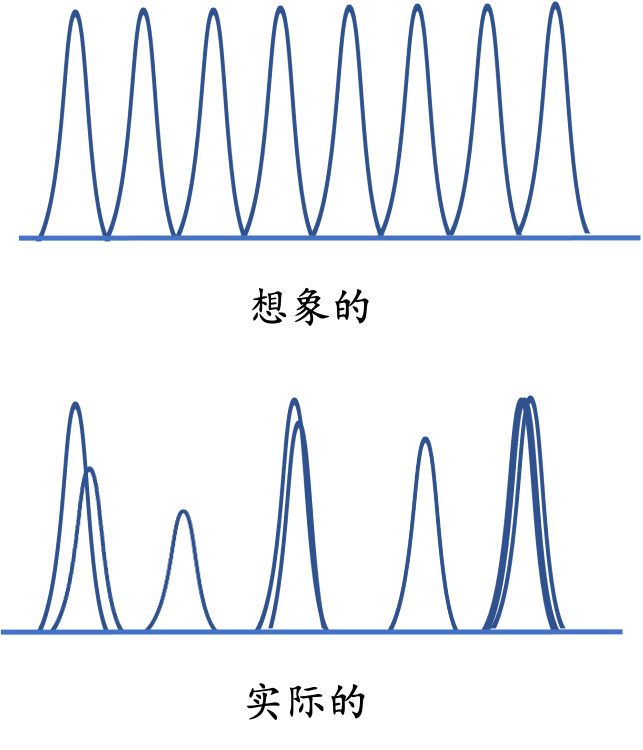
\includegraphics[width=0.35\textwidth]{figs/17.png}
 \end{center} 
\end{frame}

\begin{frame}
 \frametitle{光子计数率}
    光子流量: 
 \[ \varPhi =  \frac{P}{\hbar \omega} = \frac{I A}{\hbar \omega} \, \text{photons} \cdot s^{-1}  \]
    设备的量子效率 ($\eta$), 计数窗口时长为T, 则能被计数的平均光子数: 
    \[\overline{N}(T)=\eta \varPhi T=\frac{\eta P T}{\hbar \omega}\]
    设备的计数率 (count rate): 
    \[ R= \frac{\overline{N}(T)}{T} = \frac{ \eta P }{\hbar \omega} = \eta\varPhi \, \text{counts} \cdot s^{-1} \]
\end{frame}

\begin{frame}
 \frametitle{}
 定性分析: \\ {\vspace*{0.6em}}
      弱光计数:  通常, 量子效率 ($\eta$)约为 10\%, 计数率(R)上限约为 $10^6$ (存在死时间,约为 $1\mu s$), 因此用这种方法能计数的光场强度(P) 上限约为 $10^{-12} W $  \\  {\vspace*{0.6em}}
 定量分析: \\ {\vspace*{0.6em}}
      设一光束的光子能量为 $2.0 eV$, 光流强度为 $1 nW$, 则光子流量: 
      \[ \varPhi =  \frac{P}{\hbar \omega} = \frac{10^{-9}}{2.0 \times 1.6 \times 10^{-19}} = 3.1 \times 10^{9} \, \text{photons} \cdot s^{-1}  \]
      取光速$c=3\times 10 ^8 \, \text{m} \cdot s^{-1} $ , 表明每3米长的光束约中含31个光子. \\ 
      取计数时长 $T= 1 ns$, 对应的光束长度为 $30 cm$, 所含的光子数目约为 $3.1$, 因此光场必须量子化. \\ 
\end{frame}

\begin{frame}
      \frametitle{}
      把光分成多个$30 cm$的光束, 并不是每个光束都含$3.1$个光子, 其统计波动有可能是比较大的, 比如 \\
      \[ 0, 1, 2, 0, 6, 10, 0, 0, \cdots  \]
      如果光束长度为 $3 cm$, 其所含的光子数为$0.31$, 则光子数分布大约长这样:
      \[0,0,1, 1, 0, 0, 0, 1, 2, 0, 0, 0, \cdots \]
      此时, {\color{red}{光子的统计分布}}对计数的影响是决定性的
\end{frame}

\section{ 2. 三类统计光场}

\begin{frame}
 \frametitle{推导}
      考虑经典单色光场: 
      \[ E(x,t) = E_0 \sin (k x - \omega t + \varphi )\]
      一个理想的单模激光器发出的正是这种光, 称为相干光. 它的能量(光强)为:
      \[ <I> = \frac{1}{2} c \epsilon_0 n E_0 ^2\]
      考虑一个长为 L 光束, 其光流强度P是常数, 则所含的平均光子数为:
      \[\overline{n} = \varPhi \cdot \frac{L}{c} \]
      现在把它分成N段, 每段长度为 $L/N$, 当 $N\gg \overline{n} $时, 在不计一段有多个光子的低概率事件条件下,则在某段找到一个光子的概率为 
      \[ p= \frac{\overline{n}}{N} \] 
      现在的情况就是有 $n$ 个段含(一个)光子, (N-n)段不含光子. 
\end{frame}

\begin{frame}
      \frametitle{}
      ~\\
      这是一个N个独立的成功(含光子)/失败(不含光子)试验模型, 每次试验成功的概率为$p$, 则成功次数($n$)的离散概率分布服从二项分布
      \[ P(n) = C^n _N  p^n (1-p)^{N-n} \]
    \begin{center}
             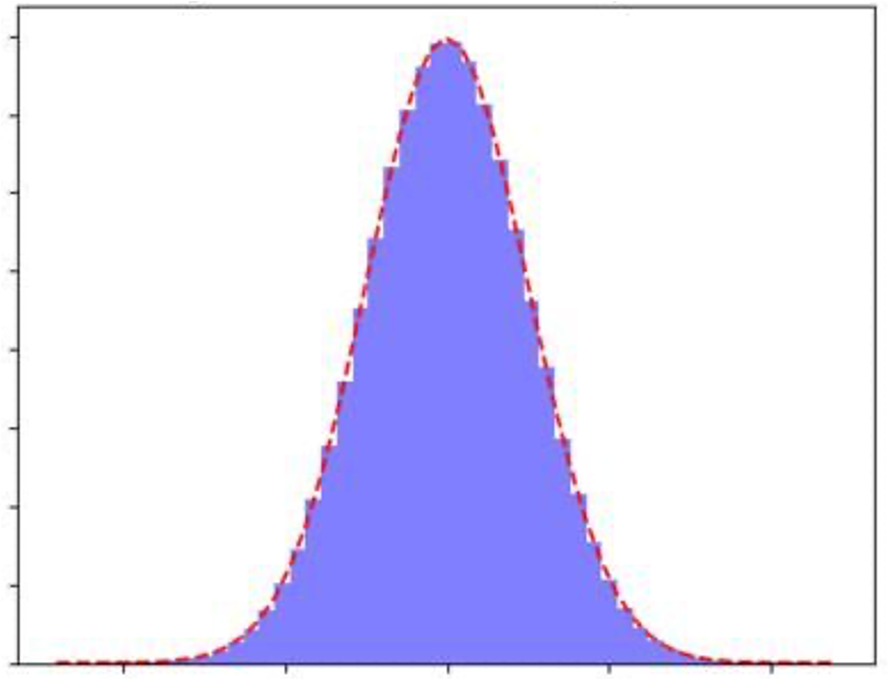
\includegraphics[width=0.5\textwidth]{figs/18.png}
    \end{center}
\end{frame}

\begin{frame}
      \frametitle{}
    把 $p= \dfrac{\overline{n}}{N}$ 代入, 有
      \[\begin{aligned}
          P(n) &= C^n _N  p^n (1-p)^{N-n} \\ 
             &= \frac{N!}{n! (N-n)!} p^n (1-p)^{N-n} \\ 
             &=  \frac{N!}{n! (N-n)!} (\frac{\overline{n}}{N} ) ^n (1-\frac{\overline{n}}{N})^{N-n} \\ 
             &= \frac{1}{n!} \left(\frac{N!} {(N-n)!N^n} \right) \overline{n}^n (1-\frac{\overline{n}}{N})^{N-n}  , 
      \end{aligned}\]
      取 $ N \to \infty , \cdots $
    \end{frame}

\begin{frame}
 \frametitle{}
    利用斯特林公式 
       \[\lim _{N \rightarrow \infty}[\ln N !]=N \ln N -N \]
    有: 
       \[\begin{aligned}
        \lim _{N \rightarrow \infty}\left[ \ln \left(  \frac{N!} {(N-n)!N^n} \right) \right]  &=  0 \\ 
        \lim _{N \rightarrow \infty}\left(  \frac{N!} {(N-n)!N^n} \right) &= 1  \qquad  \cdots (1)
    \end{aligned}\]
    利用公式 
    \[\lim _{N \rightarrow \infty} \left( 1-\frac{1}{N} \right)^N =\frac{1}{e}\]
    \[\begin{aligned}
        \lim _{N \rightarrow \infty} \left(1-\frac{\overline{n}}{N} \right)^{N-n}&=   \lim _{N \rightarrow \infty} \left(1-\frac{1}{N / \overline{n}} \right)^{(N / \overline{n}) \overline{n}}\\ 
         & = e^{-\overline{n}} \qquad  \cdots (2)
    \end{aligned}\]
\end{frame}

\begin{frame}
 \frametitle{}
      把(1)(2)代回, 有: 
      \[\begin{aligned}
        P(n) &= \frac{1}{n!} \overline{n}^n e^{-\overline{n}}  \\ 
        &= \frac{\overline{n}^n}{n!} e^{-\overline{n}}, \qquad (n=0, 1, 2, \cdots )
    \end{aligned}\]
    正是相干光场Fock态表中推导的泊松公布!, 且有:
    \[ \overline{n}= \left|\alpha\right|^2\]
    说明: 相干态光场是真随机等概率分布光场
\end{frame}

\begin{frame}
 \frametitle{定性分析}
     (1)  泊松公布要求试验次数(n) 为非负整数. \\ 
     {\Bullet}光子数只能是非负整数 \\ {\vspace*{0.3em}}
     (2)  泊松公布要求每次试验成功的概率相同. \\ 
     {\Bullet}随着N的增加, 光束在能量空间被分成一个个的波包, 相干态光子真随机等概率分布. \\ {\vspace*{0.3em}}
     (3)  取 $ N \to \infty $ 相当于经典长度无限可分. 有量子长度最小, 到达最小长度,即取得最大的N
     (4)  泊松公布要求每次试验是相互独立的. 即前一次试验结果不影响后面的试验. \\ 
     {\Bullet}光子是玻色子, 前一个光子的占据情况不影响后一个光子. \\ {\vspace*{0.3em}}
\end{frame}

\begin{frame}
 \frametitle{定量分析}
    * 分布的归一性: 
    \[\begin{aligned}
        P(n) &= \frac{\overline{n}^n}{n!} e^{-\overline{n}} \\ 
        \sum_{n=0} ^{\infty} P(n) &= \sum_{n=0} ^{\infty}\frac{\overline{n}^n}{n!} e^{-\overline{n}}  \\ 
        &= e^{-\overline{n}} \sum_{n=0} ^{\infty}\frac{\overline{n}^n}{n!} \\ 
        &= e^{-\overline{n}} \left( 1+ \overline{n} + \frac{\overline{n}^2}{2!} +\frac{\overline{n}^3}{3!} + \cdots \right) \\ 
        &= e^{-\overline{n}} \times e^{\overline{n}}  \\ 
        &= 1
    \end{aligned}\]   
\end{frame}

\begin{frame}
 \frametitle{}
  (1) 密度矩阵: 
  \[\begin{aligned} 
 \rho &=\rl{\alpha}{\alpha} \\ 
 &= \sum P(n) \rl{n}{n} \\ 
 & = \sum \frac{\overline{n}^n}{n!} e^{-\overline{n}} \rl{n}{n}  \\ 
 & = \sum \frac{\left|\alpha\right|^{1n}}{n!} e^{-\left|\alpha\right|^2} \rl{n}{n}  \\ 
\end{aligned}\] 
\end{frame}

\begin{frame}
 \frametitle{}
 (2) 均值:
 \[\begin{aligned} 
    \overline{n}  \equiv  Tr(\rho a^{\dagger} a) & \equiv  \sum_{n=0} ^{\infty} n  P(n) \\ 
    &= e^{-\overline{n}} \sum_{n=0} ^{\infty} n \frac{\overline{n}^n}{n!} \\ 
    &= e^{-\overline{n}} \left( 0+ \overline{n} + 2\frac{\overline{n}^2}{2!} +3\frac{\overline{n}^3}{3!} + \cdots \right) \\  
    &= \overline{n} e^{-\overline{n}} \left( 1+ \overline{n} + 2\frac{\overline{n}^2}{2!} +3\frac{\overline{n}^3}{3!} + \cdots \right) \\ 
    &= \overline{n} e^{-\overline{n}} \times e^{\overline{n}}  \\ 
    &= \overline{n} 
\end{aligned}\]     
\end{frame}

\begin{frame}
 \frametitle{}
   (3) 递推式: 
 \[\begin{aligned}
     P(n) &= \frac{\overline{n}^n}{n!} e^{-\overline{n}} \\ 
     &= \frac{\overline{n}^{n-1} \overline{n} }{(n-1)! n} e^{-\overline{n}} \\ 
     &= \frac{\overline{n}}{n}\frac{\overline{n}^{n-1}  }{(n-1)! } e^{-\overline{n}} \\ 
     &= \frac{\overline{n}}{n} P(n-1)\\ 
 \end{aligned}\]   
  表明:
  \begin{enumerate}
      \item $P(n)> P(n-1), \text{if} \quad  \overline{n}> n $
      \item $P(n)< P(n-1), \text{if} \quad \overline{n}< n $
  \end{enumerate}
\end{frame}

\begin{frame}
 \frametitle{}
     (4) 方差(variance): (涨落)
      \[\begin{aligned}
        Var(n) &= \overline{ (\Delta n)^2 }  \\ 
        &= \overline{ n^2} - \overline{n}^2 \\
        &= \sum_{n=0} ^{\infty} n^2 P(n) -\overline{n}^2 \\ 
        &= \sum_{n=0} ^{\infty} (n^2-n) +n P(n) -\overline{n}^2 \\ 
        &= \sum_{n=0} ^{\infty} n(n-1) P(n) + \overline{n} -\overline{n}^2 \\
    \end{aligned}\]  
\end{frame}

\begin{frame}
 \frametitle{}
 \[\begin{aligned}
    \sum_{n=0} ^{\infty} n(n-1) P(n)  & =  \sum_{n=0} ^{\infty} n(n-1) \frac{\overline{n}^n}{n!} e^{-\overline{n}}  \\
    &= e^{-\overline{n}} \sum_{n=0} ^{\infty} n(n-1) \frac{\overline{n}^n}{n!} \\ 
    &= e^{-\overline{n}} (0+0+ 2 \frac{\overline{n}^2}{2!} +  6 \frac{\overline{n}^3}{3!} + \cdots  ) \\ 
    &= \overline{n}^2 e^{-\overline{n}} (1 +  6 \frac{\overline{n}^1}{3!} + 12 \frac{\overline{n}^2}{4!}  \cdots  ) \\ 
    &= \overline{n}^2 e^{-\overline{n}} (1+ \overline{n} +  2 \frac{\overline{n}^2}{2!} + 3 \frac{\overline{n}^3}{3!}  \cdots  ) \\ 
    &= \overline{n}^2 e^{-\overline{n}} \sum_{n=0} ^{\infty} \frac{\overline{n}^n}{n!} = \overline{n}^2 \sum_{n=0} ^{\infty}  P(n)\\ 
    & = \overline{n}^2
\end{aligned}\]  
\end{frame}

\begin{frame}
    \frametitle{}
         \[\begin{aligned}
            \overline{ (\Delta n)^2 }  &= \sum_{n=0} ^{\infty} n(n-1) P(n) + \overline{n} -\overline{n}^2 \\
           &= \overline{n}^2  + \overline{n} -\overline{n}^2 \\ 
           &= \overline{n}
       \end{aligned}\]  
   \end{frame}

   \begin{frame}
    \frametitle{}
     (5) 标准偏(standard deviation)
     \[ \Delta n = \sqrt{\overline{ (\Delta n)^2 }}  = \sqrt{\overline{n}}  =\left|\alpha\right|  \]
     波动(fluctuations):
     \[ \frac{\Delta n}{n}\]
     随着光子平均数的增大, 统计波动变得越来越小
\end{frame}

\begin{frame}
      \frametitle{特点: 平均粒子数唯一决定泊松光场的数态分布}
      \[P(n) = \frac{\overline{n}^n}{n!} e^{-\overline{n}}, \qquad \overline{ (\Delta n)^2 } = \overline{n}, \qquad  \Delta n = \sqrt{\overline{n}}, \qquad \overline{n}= \left|\alpha\right|^2\]
       \begin{center}
            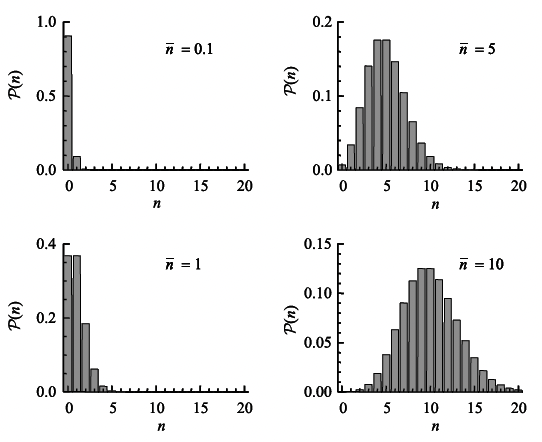
\includegraphics[width=0.53\textwidth]{figs/2022-05-06-09-01-55.png}
       \end{center}
   \end{frame}

%%%%%%%%%%%%%%%%%%%%%%%%%%%%%%%%%%%%%%%%%%%%%%%%%%%%%%%%%%%%%%%%%%%
\begin{frame}
    \frametitle{课堂作业}
     \begin{block}{ 1. An attenuated beam from an argon laser operating at
        514 nm (2.41 eV) with a power of 0.1 pW is detected with a photoncounting
        system of quantum efficiency 20\% with the time interval set at
        0.1 s. \\
        {\hspace*{1.5em}} Calculate (a) the mean count value, and (b) the standard deviation
        in the count number.}
     \end{block}
\end{frame}
%%%%%%%%%%%%%%%%%%%%%%%%%%%%%%%%%%%%%%%%%%%%%%%%%%%%%%%%%%%%%%%%%%%
 
\begin{frame}
 \frametitle{}
      \解~激光是相干光,服从泊松分布\\ 
      光子流量: 
      \[ \varPhi =  \frac{P}{\hbar \omega} = \frac{10^{-13}}{2.41 \times 1.6 \times 10^{-19}} = 2.59 \times 10^{5} \, \text{photons} \cdot s^{-1}  \]
      平均粒子数: 
      \[\overline{n}(T)=\eta \varPhi T= 0.2 \times 2.59 \times 10^{5} \times 0.1 =  5180 \]
      标准偏: 
      \[ \Delta n = \sqrt{\overline{n}} = 72   \]
\end{frame}

\begin{frame}
 \frametitle{三种统计}
      一个完美的相干光场,光子数服从泊松分布规律. 特点:  \[ \Delta n = \sqrt{\overline{n}}    \]
      因此, 基于标准偏与平均光子数的关系, 光场统计分为三类:
      \begin{enumerate}
          \item 亚泊松统计 (sub-Poissonian statistics) 
          \[ \Delta n < \sqrt{\overline{n}}    \]
          \item 泊松统计 (Poissonian statistics)
          \[ \Delta n = \sqrt{\overline{n}}    \]
          \item 超泊松统计 (super-Poissonian statistics)
          \[ \Delta n > \sqrt{\overline{n}}    \]
      \end{enumerate}
\end{frame}

\begin{frame}
 \frametitle{}
 \begin{center}
    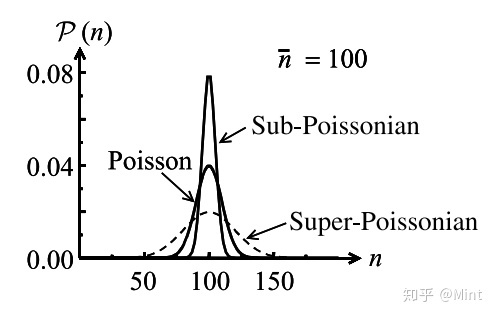
\includegraphics[width=0.6\textwidth]{figs/2022-05-06-10-46-42.png}
\end{center}
方差: 越小, 分布越集中, 说明系统越稳定. 因此, 稳定性关系为: \\ 
\[\text{亚泊松统计} > \text{泊松统计} > \text{超泊松统计} \]
\end{frame}

\begin{frame}
 \frametitle{三种光场}
 \begin{enumerate}
    \item 亚泊松光场: 非经典光场 (单光子源, 压缩态,光子反聚束, Fock态光 ,$\cdots$)
    \[ 0 \leq \Delta n < \sqrt{\overline{n}}    \]
    \item 泊松光场: 相干光场面(理想激光器)  
    \[ \Delta n = \sqrt{\overline{n}}    \]
    \item 超泊松光场: 经典光场(非理想激光器, 混沌光束, 光子聚束, 热辐射场,$\cdots$ )
    \[ \Delta n > \sqrt{\overline{n}}    \]
\end{enumerate}
    * 相干光做为泊松光是最接近经典光的量子光, 也是最接近量子光的经典光! \\ 
    * 非经典光压缩了相干光的展宽(压缩态); 相干光的展宽对应着恒定光强~ $I(t)=I(0)$ ; 经典光阔展了相干光的展宽,对应非恒定光流强度~ $I(t) \not = I(0)$, 即存在光子数波动 . 
\end{frame}

\begin{frame}
 \frametitle{~1. 单模热光场}
    热体辐射的电磁场称为热光场, 也称黑体辐射场. \\ 
    黑体可看成一系列的谐振子. 考虑一个频率为$\omega$的谐振子激发的单模光场, 能量为:
    \[ E_n = (n+\frac{1}{2}) \hbar \omega \] 
    考虑光子数服从玻尔兹曼分布
    \begin{equation*}
        P(n) =\frac{N_{n}}{N}=\frac{\exp \left(-\frac{E_{n}}{k_B T}\right)}{\sum_{n} \exp \left(-\frac{E_{n}}{k_B T}\right)}
    \end{equation*}
\end{frame}

\begin{frame}
 \frametitle{}
 代入能量(不考虑真空能):
    \[\begin{aligned}
     P(n) &=\frac{\exp \left(-\frac{n \hbar \omega }{k_B T}\right)}{\sum_{n} \exp \left(-\frac{n \hbar \omega }{k_B T}\right)} \\ 
     &= \frac{\exp^n \left(-\frac{\hbar \omega }{k_B T}\right)}{\sum_{n} \exp^n \left(-\frac{\hbar \omega }{k_B T}\right)} \\ 
     &= \frac{x^n}{\sum_{n} ^\infty x^n } \\ 
     x&= \exp \left(-\frac{\hbar \omega }{k_B T}\right) <1
    \end{aligned} \]
运用等比列数列求各公式
\[ S_n= \frac{a_1(1-q^n)}{1-q} \]
    \[\sum_{n} ^\infty x^n = \frac{x^0(1-x^n)}{1-x} = \frac{1}{1-x}\] 
\end{frame}

\begin{frame}
 \frametitle{}
 \[\begin{aligned}
    P(n) &= \frac{x^n}{\sum_{n} ^\infty x^n } \\ 
    &= x^n (1-x) \\ 
   \end{aligned} \]
   \[\begin{aligned}
    \overline{n} &= \sum_{n} ^\infty  n P(n)  \\ 
    &= \sum_{n} ^\infty  n x^n (1-x) \\ 
    &= (1-x)x \frac{\mathrm{d} }{\mathrm{dx}}\left( \sum_{n} ^\infty x^n \right)  \\
    &=  (1-x)x \frac{\mathrm{d} }{\mathrm{dx}}\left( \frac{1}{1-x} \right) \\
    &=  (1-x)x \frac{1} {1-x^2} = \frac{x}{1-x} \\ 
   \end{aligned} \]
\end{frame}

\begin{frame}
    \frametitle{}
    \[\begin{aligned}
        x & = \frac{\overline{n}}{\overline{n}+1} \\ 
        &~\\
        P(n) &= x^n (1-x) \\ 
        &=  \frac{1}{\overline{n}+1}\left( \frac{\overline{n}}{\overline{n}+1} \right)^n \\ 
        &=  \frac{\overline{n}^n}{(1+\overline{n})^{n+1}} \\ 
        &= \left( 1-\exp(-\frac{\hbar \omega}{k_B T} )
  \right) \exp(-n \frac{\hbar \omega}{k_B T}) 
      \end{aligned} \]
    称为玻色-爱因斯坦分布. \\  {\vspace*{2.3em}}
\end{frame}

\begin{frame}
 \frametitle{特点分析}
  (1) 分布
  \[ P(n) =\frac{1}{\overline{n}+1}\left( \frac{\overline{n}}{\overline{n}+1} \right)^n \]  
  最大值总出现在$n=0$处,  随着n的增加, 呈指数衰减.
    \begin{center}
         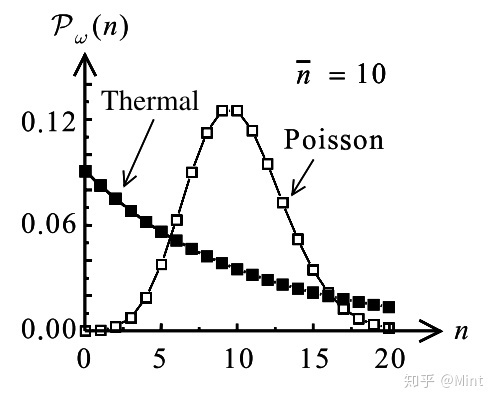
\includegraphics[width=0.4\textwidth]{figs/2022-05-06-14-46-00.png}
    \end{center}    
\end{frame}

\begin{frame}
    \frametitle{}   
    (2) 密度算符 
    \[ \begin{aligned}
        \rho &= \sum _n P(n) |n\left\rangle \right\langle n| \\
        &= \left( 1-\exp(-\frac{\hbar \omega}{k_B T} )
        \right) \sum _n \exp(-n \frac{\hbar \omega}{k_B T}) |n\left\rangle \right\langle n| \\ 
        &= \left( 1-\exp(-\frac{\hbar \omega}{k_B T} )
        \right) \exp(- \frac{\hbar \omega}{k_B T} a^{\dagger} a) \\
        &= \sum_n \frac{(\overline{n})^n}{(1+\overline{n})^{n+1}} |n\left\rangle \right\langle n| \\
        &= \frac{(\overline{n})^{a^{\dagger} a}}{(1+\overline{n})^{a^{\dagger} a+1}} 
    \end{aligned}\] 
\end{frame}

\begin{frame} 
\frametitle{}
    (3) 均值: (正是统计物理学的玻色分布, 化学势 $\mu=0 $)
    \[ \overline{n} \equiv Tr(\rho a^{\dagger} a) = \frac{x}{1-x} = \frac{1}{\exp(\hbar \omega / k_B T) -1}  \] 
     * 均值与温度存在直接的函数关系! \\ 
     ~\\ 
    (4) 方差(涨落):
    \[ Var(n) \equiv \overline{ (\Delta n)^2 } \equiv \overline{ n^2 } - \overline{ n }^2  = \overline{ n }^2 + \overline{ n }\]   
    表明热光场的量子涨落比相干光大出一个$\overline{ n }$ 
   \end{frame}

   \begin{frame}
    \frametitle{}
        计算细节:
    \[\begin{aligned}
        \overline{n^2} &= \sum_{n} ^\infty  n^2 P(n)  \\ 
        &= \sum_{n} ^\infty  n^2 P(n) \\ 
        &= \sum_{n} ^\infty  (n^2-n +n) P(n) \\ 
        &= \sum_{n} ^\infty  (n-1)n  P(n)  + \sum_{n} ^\infty  n  P(n)  \\    
        &= \overline{(n-1)n}  + \overline{n}   
    \end{aligned} \]     
   \end{frame}

   \begin{frame}
    \frametitle{}
    \[\begin{aligned}
        \overline{(n-1)n } &= \sum_{n} ^\infty  (n-1)n  P(n)   \\ 
        &= \sum_{n} ^\infty  (n-1)n  x^n (1-x)  \\    
        &= (1-x)x^2 \frac{\mathrm{d}^2 }{\mathrm{dx^2}}\left( \sum_{n} ^\infty x^n \right)  \\
        &=  (1-x)x \frac{\mathrm{d}^2 }{\mathrm{dx^2}}\left( \frac{1}{1-x} \right) \\
        &=  2 \overline{n}^2\\ 
    \end{aligned} \]   
     \[ Var(n) \equiv \overline{ n^2 } - \overline{ n }^2  = \overline{(n-1)n}  + \overline{n} - \overline{ n }^2= \overline{ n }^2 + \overline{ n }\]  
   \end{frame}

   \begin{frame} 
    \frametitle{}
    黑体辐射场的能量密度由普朗克公式给出:
    \[\begin{aligned}
        \rho(\omega, T) d \omega &=\frac{\hbar \omega ^3}{\pi ^2 c^{3}} \frac{1}{e^{\hbar \omega / K_B T}-1} d \omega \\ 
        &= \frac{\hbar \omega ^3}{\pi ^2 c^{3}} d \omega \overline{n}  \\
        &= \frac{ \omega ^2}{\pi ^2 c^{3}} \overline{\varepsilon}(\omega) d \omega \\ 
        &= g(\omega)d \omega \overline{\varepsilon}(\omega)  
    \end{aligned}\]
    普朗克公式给出的正是光子数分布和光子数密度
   \end{frame}

   \begin{frame} 
    \frametitle{}
     根据统计物理力学, 热涨落源于能量对时间的微分
    \[\begin{aligned}
        \overline{ (\Delta E)^2 }  &= k_B T^2 \frac{\partial \overline{E} }{\partial T } \\ 
        \overline{ (\Delta E)^2 } d \omega &= k_B T^2 \frac{\partial  }{\partial T } (V \rho(\omega, T)  d \omega)  \\
   &= k_B T^2 V d \omega \frac{\partial \rho(\omega, T) }{\partial T } \\ 
   &= (\hbar \omega \rho  + \frac{\pi ^2 c^{3}}{\omega ^2} \rho^2) V d \omega
    \end{aligned} \]    
   \end{frame}

   \begin{frame} 
    \frametitle{}
    热涨落也源于粒子数的涨落
    \[\begin{aligned}
        \overline{ (\Delta E)^2 } d \omega &= g(\omega)d \omega \times \overline{ (\Delta \varepsilon)^2 } \times V \\ 
        &= \frac{ \omega ^2}{\pi ^2 c^{3}} d \omega \overline{ (\Delta (n\hbar \omega))^2 } \times V \\ 
        &= \frac{ \omega ^2}{\pi ^2 c^{3}} \overline{ \Delta (n)^2 } (\hbar \omega)^2 V d \omega 
    \end{aligned} \]  
    两式比较, 得:
    \[\begin{aligned}
        \overline{ \Delta (n)^2 } &=  \frac{\pi ^2 c^{3}}{\hbar \omega ^3}\rho + (\frac{\pi ^2 c^{3}}{\hbar \omega ^3}\rho )^2 \\ 
        &=  \frac{\pi ^2 c^{3}}{\hbar \omega ^3} \frac{\hbar \omega ^3}{\pi ^2 c^{3}} \overline{n}  + (\frac{\pi ^2 c^{3}}{\hbar \omega ^3}\frac{\hbar \omega ^3}{\pi ^2 c^{3}} \overline{n}  )^2 \\ 
        &= \overline{n} + \overline{n}^2
    \end{aligned} \]
    体现了涨落的波粒二象性本质: 粒子性项 $\overline{ n }$,  波动性项 $\overline{ n }^2$ 
   \end{frame}

   \begin{frame} 
    \frametitle{}
    * 若 n 是连续变量, 则应只体现波动性. 
    \[  P(n) =\frac{N_{n}}{N}=\frac{\exp \left(-\frac{n\hbar \omega }{k_B T}\right)}{ \int_{n=0} ^\infty dn \exp \left(-\frac{n\hbar \omega}{k_B T}\right)} = \frac{e^{-nx}}{\int_{n=0} ^\infty  e^{-nx} dn}\]
    \[ \overline{n } = \int_{n=0} ^\infty n P(n)  dn = \int_{n=0} ^\infty n \frac{e^{-nx}}{\int_{n=0} ^\infty  e^{-nx}dn}  dn\]
    \[ \overline{n^2 } = \int_{n=0} ^\infty n^2 \frac{e^{-nx}}{\int_{n=0} ^\infty  e^{-nx}dn}  dn = 2 \overline{n }^2 \]
    \[ Var(n) \equiv \overline{ n^2 } - \overline{ n }^2  = 2\overline{ n }^2 - \overline{ n }^2 = \overline{ n }^2 \] 
    只有波动性带来的项 $\overline{ n }^2$ , 没有了粒子性带来的项 $\overline{ n }$  
\end{frame}

\begin{frame} 
    \frametitle{~2.多模热光场}
    单模热光场是一阶相干的, (任何单模激发的光场都是一阶相干的) . \\
    实际上, 热激发的是多模场, 设模式数目为$n_k$, 则密度算符 
    \[ \begin{aligned}
        \rho &= \sum_{\{n_k\}} |\{n_k\} \left\rangle \right\langle \{n_k\} | \prod_k
        \frac{(\overline{n_k})^{n_k}}{(1+\overline{n_k})^{n_k+1}} \\
    \end{aligned}\] 
    由于各模相位不同, 削弱了波动性带来的涨落:
    \[ \overline{ (\Delta n)^2 } = \frac{\overline{ n }^2}{n_k} + \overline{ n } \] 
    当  $n_k \to \infty$, 热光场趋于泊松分布. \[ \overline{ (\Delta n)^2 } = \overline{ n }\] 
\end{frame}

\begin{frame} 
 \frametitle{~3. 混沌光束}
 实验室常用的两种光源:
 \begin{enumerate}
     \item 激光器: 相干泊松光
     \item 气体放电管: 部分相干混沌光
 \end{enumerate}
   \begin{center}
        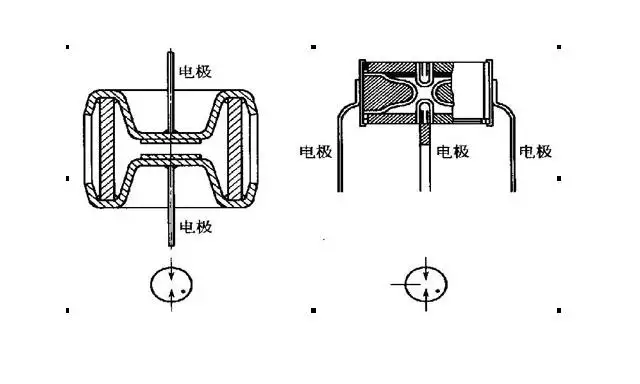
\includegraphics[width=0.7\textwidth]{figs/2022-05-07-11-10-12.png}
   \end{center}
\end{frame}

\begin{frame}
 \frametitle{}
 混沌光束是部分相干光, 光子流量不是常数($\varPhi (t) $) 
 探测器的计数率 (计数期内探测到的光子数):  
    \[R(t)= \int _{t=0} ^ {T} \eta \varPhi (t)  dt\]
 有均值:
\[ \overline{n}  = < R(t)> \]
\[ \overline{n^2}  = < R^2 (t)> \]
均方差:
\[\begin{aligned}
    \overline{(\Delta n)^2} &= < R^2 (t)> - < R(t)>^2 \\ 
    &= \overline{R}(t)+\overline{R}^2(t)
\end{aligned}\]
\end{frame}

\begin{frame}  
 \frametitle{分析}
 \begin{itemize}
     \Item 如果测量时间(T)与相干时间$\tau_c$ 相当, 第二项的影响会很大. 服从超泊松统计.
     \Item 如果$T\gg \tau_c$, 第二项因相位平均趋零,即波动性影响消失. 服从泊松统计.
 \end{itemize}    
\end{frame}

\begin{frame} 
 \frametitle{4. Fock态光场}
 对于相干光,光子流量是常数. 当测量时间(T)变得足够短, 短到每次测得的光子数刚好为1. 
   \begin{center}
        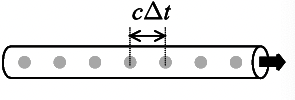
\includegraphics[width=0.4\textwidth]{figs/2022-05-07-14-58-04.png}
   \end{center}
 则相当于单光子源. 变成Fock态光场 \\
 有均值(数密度):
 \[ \overline{n}= Tr(\rho a^{\dagger} a)= n\] 
 方差 (涨落): 
 \[ Var(n) = \overline{(\Delta n)^2} =0 \]
\end{frame}

\begin{frame} 
 \frametitle{损耗导致光场统计退化}
    光束通过光学损耗材料会损失光子, 可以用光学分束器来模拟
      \begin{center}
           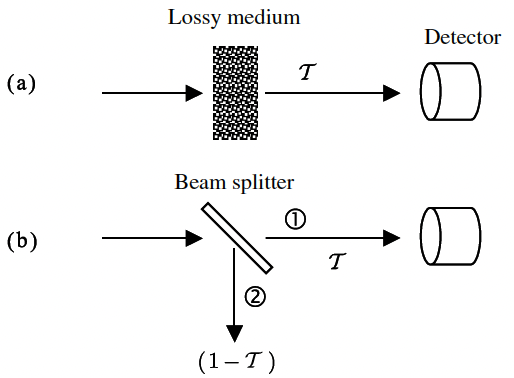
\includegraphics[width=0.6\textwidth]{figs/2022-05-07-15-10-50.png}
      \end{center}      
\end{frame}

\begin{frame} 
 \frametitle{}
    光学分束器模型有可有效表述如下现象:
 \begin{itemize}
    \Item 光源发出的光子没有被全部收集.
    \Item 光的吸收, 光的反射, 光的散射等导致的光子损失.
    \Item 光学探测器的量子效应低导致某些光子没有被探测到.
\end{itemize} 
\end{frame}

\begin{frame} 
 \frametitle{}
   \begin{center}
        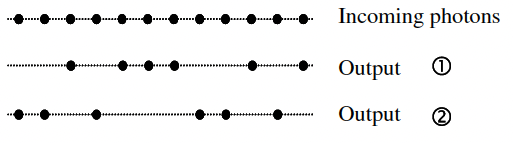
\includegraphics[width=0.7\textwidth]{figs/2022-05-07-15-17-44.png}
   \end{center}
\begin{itemize}
    \item 入射光束的光子流量是常数(相干光), 光子被光随机损耗后, 出射光束的光子流量不再是常数. 
    \item 对于透射率很小的材料, 出射光束的光子流量完全变成了关于时间的随机函数, 变成了非相干光(退相干).
\end{itemize} 
* 光场的统计特性决定于两方面: (1)  光束本身的统计特性, (2) 探测器   
\end{frame}

\section{ 3. 光的探测理论}

\begin{frame} 
 \frametitle{半经典探测理论}
 半经典理论认为: 光束是一系列电磁波构成, 也是一束光子流. 电磁波强度对应光子数
   \begin{center}
        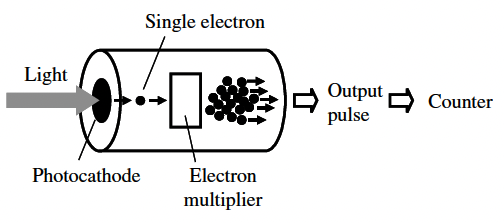
\includegraphics[width=0.7\textwidth]{figs/2022-05-07-15-48-38.png}
   \end{center}      
\end{frame}

\begin{frame} 
 \frametitle{}
    设电磁波强度为$I(t)$, 在  $ \Delta t $ 时间内,测到一次光电发射事件的概率为 
    \[ P (1:, t, t+\Delta t) = \xi I(t) \Delta t \]
    只要$ \Delta t \to 0$, 同时测得两次或两次以上的光电发射事件的概率几乎为零. 因此, 没有测到光电发射事件的概率为 
    \[ P (0:, t, t+\Delta t) = 1- P (1:, t, t+\Delta t) =1- \xi I(t) \Delta t \]
    在$0, t+ \Delta t$时间段内, 测得$n$次光电发射事件的概率为:
    \[\begin{aligned}
        P (n:, 0, t+\Delta t) &= P (n:, 0, t) P (0:, t, t+\Delta t) + P (n-1:, 0, t) P (1:, t, t+\Delta t) \\ 
        &= P (n:, 0, t) (1- \xi I(t) \Delta t ) + P (n-1:, 0, t) \xi I(t) \Delta t 
    \end{aligned}\]
    
\end{frame}

\begin{frame} 
 \frametitle{}
 令 \[ P_n (t)= P (n:, 0, t), \qquad P_n (t+\Delta t)=P (n:, 0, t+\Delta t)\]
 上式可改定为:
 \[ \frac{P_n (t+\Delta t)- P_n (t)}{\Delta t } =\xi I(t) [P_{n-1} (t) -P_{n} (t) ]  \]  
 令$ \Delta t \to 0$, 得微分形式:
 \[ \frac{\mathrm{d}P_n (t)}{\mathrm{d}t} =\xi I(t) [P_{n-1} (t) -P_{n} (t) ]  \]
 令$P_0 (0)=0$, 解方程得:
\[ P_n (t) = \frac{\left[ \int_0 ^t \xi I(t') d t' \right]^n }{n!} \mathrm{e}^{- \int_0 ^t \xi I(t') d t'  } \]
\end{frame}

\begin{frame} 
 \frametitle{}
    对于相干光, $I(t)=I(0)$, 光电发射事件均数为:
    \[ \overline{n} = \xi I(0) t = Ct\]
    上式简化为:
    \[ \begin{aligned}
        P_n (t) &= \frac{(Ct)^n }{n!} \mathrm{e}^{- Ct }\\
        &= \frac{\overline{n}^n }{n!} \mathrm{e}^{- \overline{n} }\\
    \end{aligned}\] 
    正是泊松分布! 这说明: \\ \vspace*{0.3em}
    \begin{itemize}
        \item 光电发射就是一个电子随机从光束吸收量子化能量的过程, 如果光强与时间无关. 
        \item 从半经典理论不可能得到亚泊松分布的光场, 因为强度若与时间相关,则必然超泊松分布
        \item 要考虑单光子源,压缩光, 光子反聚束, Fock态光等,必发展全量子探测理论 
    \end{itemize}
\end{frame}

\begin{frame} 
 \frametitle{全量子探测理论}
 全量子探测理论依赖于全量子的光与物质的相互作用. 这里, 我们只给出基本结论: 探测器的量子效率
 \[ \eta = \overline{N} /\overline{n} \]
 探测器记数的方差与光子数方差之间的关系:
 \[ (\Delta N )^2 = \eta^2 (\Delta n )^2 + \eta(1-\eta)\overline{n}  \]
 分析: 
    \begin{enumerate}     
    \item $\eta=1$, $\Delta N= \Delta n$. 理想探测如实描述游光场统计特征
     \item $(\Delta n )^2=\overline{n}$, $\Delta N= \eta \overline{n}= \overline{N} $. 对于泊松光场,探测器总给出泊松分布,无关量子效率的大小.
     \item $\eta \ll 1$, $\Delta N= \eta \overline{n}= \overline{N}$. 量子效率极低的探测器总给出泊松分布, 无关光场本身的统计特性.
    \end{enumerate}
\end{frame}

\begin{frame} 
 \frametitle{光电探测的噪声}
      光电流:
      \[ i=  \eta e \varPhi = \eta e \frac{P}{\hbar \omega} \]
      响应率: 
      \[ \frac{i}{P}= \frac{\eta e }{\hbar \omega} \]
      光子数的波动导致光电流是含时的:
      \[ i(t)=  \overline{i} + \Delta i (t) \]
      另外, 电路本身有噪声, 因此, 总的噪声强度为:
      \[ P_{\text{noise}}(t)= (\Delta i (t))^2 R_L \]
\end{frame}

\begin{frame} 
 \frametitle{}
 对于泊松光
 \[ (\Delta N)^2 = \overline{N} \qquad \to \qquad (\Delta i)^2 \propto \overline{i} \]
 经傅里叶变换, 从时域(t)变成频率(f), 噪声公式
 \[(\Delta i)^2 = 2e (\Delta f) \overline{i} \]
 \[ P_{\text{noise}}(f)= 2e R_L (\Delta f) \overline{i} \]
 噪声的两个来源: (1)频率波动$(\Delta f)$, (2) 光电流波动 $\overline{i}$
\end{frame}

\begin{frame} 
      \frametitle{}   
    \begin{center}
        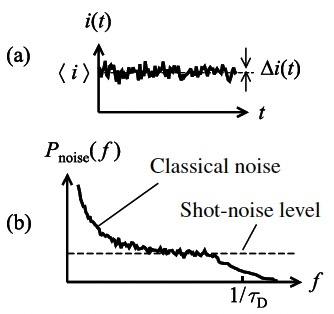
\includegraphics[width=0.35\textwidth]{figs/2022-05-08-09-51-35.png}
    \end{center}
    光源的经典噪声应来源于光源(激光器)的驱动电路及腔中镜片的热振动, 因此只出现在低率区. 高频区的噪声称为散粒噪声, 来源于光子统计. \\
    散粒噪声的特点: 
    \begin{enumerate}
        \item 电流方差与电流平均值成正比
        \item 噪声谱是白的,即不依赖于光子频率.
    \end{enumerate}
\end{frame}

\begin{frame} 
 \frametitle{* 增益与噪声}
      光电放大器的增益系数: $\gamma $ \\ 
      增益: G, 
      \[ G= \exp (\gamma L) \]
      (L 为光电信号线性区域的长度)\\
      信号-噪声率(SNR):
      \[\text{SNR}= \frac{\left\langle I \right\rangle^2}{\left (\langle \Delta I)^2 \right\rangle}  \]
\end{frame}

\begin{frame} 
 \frametitle{}
    量子化SNR: 
    \[\text{SNR}= \frac{\overline{n}}{\left (\langle \Delta n)^2 \right\rangle}  \]
    对于相干光:
    \[\text{SNR}= \frac{\overline{n}}{\left (\langle \Delta n)^2 \right\rangle} = \frac{\overline{n}}{\left (\langle \sqrt{\overline{n}})^2 \right\rangle} = \overline{n}\]  
    噪声系数 (NF): 
    \[\text{NF}=\frac{\text{SNR}_{in}}{\text{SNR}_{out}} = 2-\frac{1}{G} \]
\end{frame}

%%%%%%%%%%%%%%%%%%%%%%%%%%%%%%%%%%%%%%%%%%%%%%%%%%%%%%%%%%%%%%%%%%%
\begin{frame} 
    \frametitle{课外作业}
    A 10 mW He:Ne laser operating at 632.8 nm is detected with a photodiode of responsivity of 0.43 $AW^{−1}$ via a load resistor of 50 Ω. Calculate:
    \begin{enumerate}
        \item the quantum efficiency of the detector
        \item the average photocurrent
        \item the root-mean-square current fluctuations within a band-width of 100 kHz,
        \item  the noise power measured in dBm units after amplification by an
        amplifier with a power gain of 20 dB in the same 100 kHz bandwidth.
    \end{enumerate}
\end{frame}
%%%%%%%%%%%%%%%%%%%%%%%%%%%%%%%%%%%%%%%%%%%%%%%%%%%%%%%%%%%%%%%%%%%  % 光子探测与计数
%\begin{frame}
    \frametitle{前情回顾}
    \begin{itemize}
        \item 量子化光场~~真空态~~产生湮灭算符 
        \item 相干态~~ 平移算符 ~~相图
        \item 压缩态~~ 压缩算符
        \item 数态表象~~数态展开
        \item 参量下转换~~平衡零差探测 
        \item 光子计数 ~~ 亚泊松~~泊松~~超泊松光场 
    \end{itemize}     
\end{frame}

%%%%%%%%%%%%%%%%%%%%%%%%%%%%%%%%%%
\begin{frame} [plain]
    \frametitle{}
    \Background[1] 
    \begin{center}
    {\huge 第12-13讲:关联函数}
    \end{center}  
    \addtocounter{framenumber}{-1}   
\end{frame}

\section{1. 经典关联函数}
\begin{frame} 
    \frametitle{杨氏干涉实验}
    \begin{columns}
    \begin{column}[t]{0.4\linewidth}
    \begin{itemize}
        \item 光源带宽 $\Delta \omega $  
        \item 路程差 $\Delta s = |s_1 - s_2|$ 
        \item 相干条件 $\Delta s \le \dfrac{c}{\Delta \omega}$ 
        \item 相干长度 $\Delta s_{coh} = \dfrac{c}{\Delta \omega}$
        \item 相干时间 $\Delta t_{coh} = \dfrac{1}{\Delta \omega}$
    \end{itemize}
    \end{column}
    \begin{column}[t]{0.6\linewidth} 
        \begin{center}
        \includegraphics[width=1.0\textwidth]{figs/2022-06-02-14-02-17.png} 
        \end{center} 
        \end{column} 
        \end{columns} 
    \end{frame}

\begin{frame} 
\frametitle{}
    在$t$时刻, 探测器处的场
    \[ \mathbf{E}(\mathbf{r},t) = K_1\mathbf{E}(\mathbf{r}_1,t-s_1/c) + K_2\mathbf{E}(\mathbf{r}_2,t-s_2/c)\]
    测得的光强:
    \[ I (\mathbf{r}) = <|\mathbf{E}(\mathbf{r},t)|^2> = \lim_{T\to \infty} \frac{1}{T}\int_0 ^T \mathbf{E}(\mathbf{r},t)|^2 dt\]
    假设测量过程是一个平稳随机过程, 基于各态历经假说, 时间平均可转化为系综平均.
    \[ \begin{aligned}
        I (\mathbf{r}) =~&K^2 _1\mathbf{E}^2(\mathbf{r}_1,t_1) + K^2 _2\mathbf{E}^2(\mathbf{r}_2,t_2)\\
        &+ 2 Re{[K^* _1 K _2 \mathbf{E}^*(\mathbf{r}_1,t_1)\mathbf{E}(\mathbf{r}_2,t_2)]}\\
        &= I^2_1 + I^2_2 + 2\sqrt{I_1 I_2}Re{[K_1 K _2 g^{(1)}(\mathbf{x}_1, \mathbf{x}_2)]}
    \end{aligned}\] 
\end{frame}

\begin{frame} 
\frametitle{关联函数}
    式中定义了张量
    \[ \mathbf{x}= (\mathbf{r},t)\]
    和一阶关联函数
    \[g^{(1)}(\mathbf{x}_1, \mathbf{x}_2) = \frac{<\mathbf{E}^*(\mathbf{x_1}) \mathbf{E}(\mathbf{x}_2) >}{<|\mathbf{E}(\mathbf{x}_1)|^2><|\mathbf{E}(\mathbf{x}_1)|^2>}\]
    令 
    \[K_i = |K_i| e^ {i\phi_i}, \qquad g^{(1)}(\mathbf{x}_1, \mathbf{x}_2) = |g^{(1)}(\mathbf{x}_1, \mathbf{x}_2)| e^ {i\varphi_{12}}\]
    得:
    \[ I (\mathbf{r}) = I^2_1 + I^2_2 + 2\sqrt{I_1 I_2}|K_1 K _2| |g^{(1)}(\mathbf{x}_1, \mathbf{x}_2)| \cos(\varphi_{12}+ \phi_1 + \phi_2)\] 
\end{frame}

\begin{frame} 
\frametitle{}
    分析: 相位信息对应干涉
    \begin{itemize}
        \item 完全相干 $|g^{(1)}(\mathbf{x}_1, \mathbf{x}_2)|=1$
        \item 部分相干 $|g^{(1)}(\mathbf{x}_1, \mathbf{x}_2)| < 1$
        \item 不相干 $~~~|g^{(1)}(\mathbf{x}_1, \mathbf{x}_2)| =0 $
    \end{itemize}
    对于同一位置出发经过不同路程到达探测器的两束光, 有
    \[g^{(1)}(\mathbf{r}, t; \mathbf{r}, (t+\tau) )= g^{(1)} (\tau)\]
    称为自关联函数
\end{frame}

\section{2. HBT 实验}

\begin{frame} 
\frametitle{HBT 实验背景}
\begin{itemize}
    \item 1956年Hanbury Brown和Twiss两哥们想测量天狼星的直径
    \item 迈克尔逊干涉仪却测天狼星边界两束光场的干涉条纹, 结果没有干涉条纹
    \item 原因: 天狼星离地球太远(8.6光年),传播路径上的扰动导致相位信息信息混乱
    \item 哥俩想光强相对于相位稳定得多, 测测它们的光强试试
    \item 发现光强的相干性!
\end{itemize}
\end{frame}

\begin{frame} 
 \frametitle{实验原理}
   \begin{center}
        \includegraphics[width=1.0\textwidth]{figs/2022-05-08-12-30-39.png}
   \end{center}
   Nature(Nature 177, 27 (1956). Nature 178, 1046 (1956). 
\end{frame}

\begin{frame}
 \frametitle{}
 迈克耳逊恒星干涉仪原理: 相位相干 \\ 
 由于地球与恒星的距离(L)远大于恒星的直径(D), 满足角度放大条件.
 \[ \delta \theta_s =\frac{D}{L}\] 
 时间和空间相干性, 导致迈克耳逊恒星干涉仪存在角度极限:
 \[ \delta \theta_r\leq 1.22 \frac{\lambda}{d}\] 
 当 $d> 1.22 \lambda /\delta \theta_s$, 则没有干涉条纹.  \\ \vspace*{1.3em}
 因此, 当两镜片间距(d)变大到某点时,干涉条纹刚好消失, 由此可得$\theta_s$, 进而得恒星直径(D). 
\end{frame}

\begin{frame} 
 \frametitle{}
 但是$d$增大时,保持两镜片的稳定性会变得越来越困难(不稳定会导致角度误差放大). 因此, 迈克耳逊恒星干涉仪不能用来测量很大的恒星. \\ {\vspace*{2.3em}}
 计算迈克耳逊恒星干涉仪的光强
 \[ \begin{aligned}
     E&= E_k (e^{\mathbf{ik}\cdot \mathbf{r}_1}+ e^{\mathbf{ik}\cdot \mathbf{r}_2}) + E_{k'} (e^{\mathbf{ik'}\cdot \mathbf{r}_1}+ e^{\mathbf{ik'}\cdot \mathbf{r}_2}) \\ 
     I&= \kappa \left\langle E^* E \right\rangle \\
     &= \kappa \left\langle 2 \left| E_k\right|^2 + 2\left| E_{k'}\right|^2 + \left|E_k\right|^2 (e ^{i \mathbf{k}\cdot(\mathbf{r}_1-\mathbf{r}_2)+c.c.})  \right\rangle \\
 \end{aligned}\]
\end{frame}

\begin{frame} 
\frametitle{}
 取 $\left| E_{k}\right|^2 \approx \left| E_{k'}\right|^2 = I_0$, $\mathbf{r}_0 = \dfrac{\mathbf{r}_1 - \mathbf{r}_2}{2}$,    
 光强为
 \[ I = 4 \kappa I_0 \left\{ 1+\cos\left[ (\mathbf{k} + \mathbf{k}')\cdot \mathbf{r}_0\right] \cos\left( (\mathbf{k} - \mathbf{k}')\cdot \mathbf{r}_0 \right)  \right\}\]
分析: \\ 
 (1) $\mathbf{k} - \mathbf{k}'$大气的扰动相互抵消, 因此, 调节位置, 可使 \[\cos\left( (\mathbf{k} - \mathbf{k}')\cdot \mathbf{r}_0 \right)=1 \]
(2) 问题在
\[ \cos\left[ (\mathbf{k} + \mathbf{k}') \cdot \mathbf{r}_0 \right] \]
没有办法处理. 这是一个变化很快的敏感项, 大气的扰动和仪器的噪声涨落可导致其平均值归零, 从而限制了迈克耳逊恒星干涉仪的使用 
\end{frame}

\begin{frame} 
\frametitle{}
 HB-T实验革新点: \\
 \begin{enumerate}
     \item 改平面镜为凹面镱, 可以收集更多的光, 可测量更暗些的恒星
     \item 改相位干涉(关联)为强度干涉(关联), 可测量更大的恒星
 \end{enumerate}
 目前,HBT实验已成为量子光学的奠基性实验!
\end{frame}

\begin{frame} 
 \frametitle{}
    首先,要在理论上证明两光强度之间是存在关联的!   
    \begin{center}
        \includegraphics[width=0.6\textwidth]{figs/2022-05-08-13-20-54.png}
   \end{center}
   量子力学中,如果两函数不正交(内积不为零),则它们线性相关, 是有关联的.
   \[ \int \psi^*_1(\mathbf{r_1},t) \psi_2(\mathbf{r_2},t+ \tau) \mathbf{dr}dt \not = 0 \]
因此, HB-T 实验本质上是求两光场波函数的内积问题.
\end{frame}

\section{3. 半经典关联函数}

 \begin{frame} 
  \frametitle{一阶关联函数}
  根据半经典测量理论,光强为$I(\mathbf{r},t)$光照在光电探测器上, 在 $\Delta t $ 时间内, 发生光电发射事件(测得光子)的差分概率为 
\[  P (\mathbf{r},t) \Delta t = \eta \left\langle I(\mathbf{r},t) \right\rangle \Delta t \]  
代入电场强度, 有:   
\[ \begin{aligned}
    P (\mathbf{r},t) \Delta t &= \eta \left\langle I(\mathbf{r},t) \right\rangle \Delta t \\ 
    & = \eta \left\langle E^* (\mathbf{r},t) E (\mathbf{r},t)\right\rangle \Delta t \\
    &=\eta G^{1} (\mathbf{r},t) \Delta t  \\
\end{aligned}\] 
 \end{frame}

 \begin{frame} 
  \frametitle{}
  上式中,定义了对时间的内积函数:
\[ \boxed{ G^{(1)} (\mathbf{r},t) = \left\langle E^* (\mathbf{r},t) E (\mathbf{r},t)\right\rangle} = \int E^* (\mathbf{r},t) E (\mathbf{r},t) dt \]
  称为一阶关联函数, 它描述了光场的自相关性.\\ 
  \[ \begin{aligned}
    P (\mathbf{r},t) \Delta t &=\eta G^{1} (\mathbf{r},t) \Delta t  \\
   \end{aligned}\] 
   表明: 探测器发生光电发射事件的概率,用一阶关联函数描述. 
 \end{frame}

 \begin{frame}   
    \frametitle{二阶关联函数}
   如果有两个探测器, 则
    \[ \begin{aligned}
      P (\mathbf{r_1},t_1) \Delta t_1 &=\eta \left\langle E^*_1 (\mathbf{r_1},t_1) E_1 (\mathbf{r_1},t_1)\right\rangle \Delta t_1  \\
      P (\mathbf{r_2},t_2) \Delta t_2 &=\eta \left\langle E^*_2 (\mathbf{r_2},t_2) E_2 (\mathbf{r_2},t_2)\right\rangle  \Delta t_2  \\
     \end{aligned}\] 
    两探测器相互独立测量, 则两探测器都测得光子的概率为:
    \[ \begin{aligned}
        P_2 (\mathbf{r_1},t_1; \mathbf{r_2},t_2)  &= P (\mathbf{r_1},t_1) \Delta t_1 P (\mathbf{r_2},t_2) \Delta t_2\\
        &= \eta_1 \eta_2 \left\langle E^*_1 (\mathbf{r_1},t_1) E_1 (\mathbf{r_1},t_1)\right\rangle  \left\langle E^*_2 (\mathbf{r_2},t_2) E_2 (\mathbf{r_2},t_2)\right\rangle \Delta t_1 \Delta t_2 \\
    \end{aligned}\] 
    如果两探测器做联合测量, 则:
    \[ \begin{aligned}
        P_2 (\mathbf{r_1},t_1; \mathbf{r_2},t_2)  
        &= \eta_1 \eta_2 \left\langle E^*_1 (\mathbf{r_1},t_1) E_1 (\mathbf{r_1},t_1) E^*_2 (\mathbf{r_2},t_2) E_2 (\mathbf{r_2},t_2)\right\rangle \Delta t_1 \Delta t_2 \\
        &= \eta_1 \eta_2  G^{(2)} (\mathbf{r_1},t_1; \mathbf{r_2},t_2) \Delta t_1 \Delta t_2 
    \end{aligned}\]
\end{frame}

\begin{frame} 
 \frametitle{}
 上式,定义了二阶关联函数:
 \[ \boxed{ \begin{aligned}   
 G^{(2)} (\mathbf{r_1},t_1; \mathbf{r_2},t_2)  &= \left\langle E^*_1 (\mathbf{r_1},t_1) E_1 (\mathbf{r_1},t_1) E^*_2 (\mathbf{r_2},t_2) E_{2} (\mathbf{r_2},t_2)\right\rangle \\ 
 &= \left\langle I_1 (\mathbf{r_1},t_1) I_2 (\mathbf{r_2},t_2)\right\rangle
\end{aligned}} \]
它描述两不同位置的光场之间的相关性. 或者说两不同探测器测得的两光强之间的相关性. \\ 
\end{frame}

\begin{frame} 
\frametitle{}
同一位置不同时刻的两次测量的关联函数:
\[ \begin{aligned}
    G^{(2)}(\tau) &= G^{(2)}(t; t+ \tau) \\
    &= \left\langle E^* (t) E (t) E^* (t+ \tau) E (t+ \tau)\right\rangle \\
    &= \left\langle I (t)  I (t+ \tau)\right\rangle \\ 
\end{aligned}\] 
\end{frame}

\begin{frame}
\frametitle{}
归一化的关联函数为:
\[  g^{(1)} (\mathbf{r},t) =  \frac{\left\langle E^* (\mathbf{r},t) E (\mathbf{r},t)\right\rangle} {\left\langle E^* (\mathbf{r},t)\right\rangle\left\langle E (\mathbf{r},t)\right\rangle}  \]
\[ \begin{aligned}   
    g^{(2)} (\mathbf{r_1},t_1; \mathbf{r_2},t_2)  
    &= \frac{\left\langle I_1 (\mathbf{r_1},t_1) I_2 (\mathbf{r_2},t_2)\right\rangle}{\left\langle I_1 (\mathbf{r_1},t_1)\right\rangle\left\langle I_2 (\mathbf{r_2},t_2)\right\rangle}
   \end{aligned} \]
\end{frame}

 \begin{frame} 
  \frametitle{分析}
  同一时刻的相关性
  \[  g^{(2)}(0) = \frac{\left\langle I (t)  I (t+ \tau)\right\rangle} {\left\langle I (t) \right\rangle \left\langle I (t+ \tau)\right\rangle} =  \frac{\left\langle I^2 (t)  \right\rangle}{\left\langle I (t)\right\rangle^2 }  \geq 1\]
  对于相干态, $  \left\langle I^2 (t)  \right\rangle = \left\langle I (t) \right\rangle^2, \quad g^{(2)}(0) =1 $ \\ 
  对于混沌光束, $ \left\langle I^2 (t)  \right\rangle > \left\langle I(t) \right\rangle^2, \quad g^{(2)}(0) >1 $
\end{frame}

\begin{frame} 
      \frametitle{}   
  设光束的相干时间为$\tau_c$ (原子能级的寿命),当$\tau\gg \tau_c$, 没有时间相干性, 则 
  \[ I (t) = \left\langle I \right\rangle  + \Delta I (t) =  \left\langle I  \right\rangle  \] 
  \[ \begin{aligned}
    g^{(2)}(\tau) &= \frac{\left\langle I (t)  I (t+ \tau)\right\rangle }{\left\langle I (t) \right\rangle \left\langle  I (t+ \tau)\right\rangle }\\ 
    &= \frac{\left\langle \left\langle I  \right\rangle  \left\langle I  \right\rangle \right\rangle}{\left\langle I \right\rangle^2} \\
    &= 1 
\end{aligned}\]     
\end{frame}
  
 \begin{frame} 
  \frametitle{}
      对于相干态, 恒有 $ I (t)= I (0) =I$ 
      \[ \begin{aligned}
        g^{(2)}(\tau) &= \frac{\left\langle I (t)  I (t+ \tau)\right\rangle}{\left\langle I (t) \right\rangle \left\langle I (t+ \tau)\right\rangle} \\ 
        &= \frac{\left\langle I^2\right\rangle}{ \left\langle I\right\rangle ^2} \\
        &= 1   
    \end{aligned}\] 
      \begin{center}
           \includegraphics[width=0.5\textwidth]{figs/2022-05-08-15-34-39.png}
      \end{center} 
    * 半经典二阶关联函数只能描述经典光和相干光的光强相关性,不能给出非经典光的物理图像.
 \end{frame}

 \begin{frame} 
  \frametitle{}
  热辐射光场的一阶关联函数:
  \[ g^{(1)}(\tau) = \frac{\sum_k \overline{n}_k \omega_k \exp{(-i \omega_k \tau)} }{\sum_k \overline{n}_k \omega_k}, \quad g^{(2)}(\tau) =1+ \left|g^{(1)}(\tau) \right|^2\]
  对于高斯混沌光束: 
       \[g^{(2)}(\tau) =1 + e^{-\pi (\frac{\tau}{\tau_c})^2 } \]
  对于洛伦兹混沌光束
       \[g^{(2)}(\tau) =1 + e^{-2 \frac{\left|\tau\right|}{\tau_0} } \]
         \begin{center}
              \includegraphics[width=1.0\textwidth]{figs/2022-05-08-16-01-24.png}
         \end{center}
 \end{frame}

\section{3. 量子关联函数}

 \begin{frame} 
  \frametitle{ 光子HB-T实验}
         \begin{center}
              \includegraphics[width=0.8\textwidth]{figs/2022-05-08-16-13-39.png}
         \end{center}
     如光强很弱, 则要使用单光子探测器进行计数, 则应采用全量子光学方法处理
 \end{frame}

 \begin{frame} 
    \frametitle{}
    ~\\
    {\Bullet}平稳随机过程假设\\
    (1) 统计的稳定性(statistically stationary)\\ 
    对任意时间$T$,下面的联合测量概率恒成立.
         \[ P_{n}\left(x_{n}, t_{n} ; x_{n-1}, t_{n-1} ; \ldots ; x_{1}, t_{1}\right)=P_{n}\left(x_{n}, t_{n}+T ; x_{n-1}, t_{n-1}+T ; \ldots ; x_{1}, t_{1}+T\right)\]
    (2) 性质: \\ 
    时间原点选取不影响概率
    \[ P_1(x,t)=P_1(x,0)\]
    对空间的概率积分不依赖于时间原点选取
    \[ \left\langle x(t) \right\rangle = \int x P_1(x,t)dx=  \int x P_1(x,0)dx  \]
    \end{frame}

 \begin{frame} 
  \frametitle{}
  {\Bullet} 单光子探测器, 测得的光子数(计数)服从泊松分布(平稳随机过程)
       \[  P_n = \frac{\overline{n}^n }{n!} \mathrm{e}^{- \overline{n} }\]
       计数均值:
    \[ \begin{aligned}
        \overline{n} &= \sum_n n P_n\\
        &=\sum_n n \frac{\overline{n}^n }{n!} \mathrm{e}^{- \overline{n} } \\
        &= \left\langle \sum_n n \frac{(\eta I)^n }{n!} \mathrm{e}^{- \eta I }  \right\rangle \\ 
        &= \left\langle (\eta I) \frac{\mathrm{d}}{\mathrm{d}(\eta I)}\sum_n  \frac{(\eta I)^n }{n!} \mathrm{e}^{-\eta I }  \right\rangle \\
        &=  \left\langle \eta I \right\rangle = \eta \left\langle I \right\rangle
    \end{aligned}\] 
 \end{frame}

 %\begin{frame} 
 % \frametitle{}
 % 平方数均值:
 % \[ \begin{aligned}
 %   \overline{n^2} &= \sum_n n^2 P_n\\
 %   &= \sum_n n(n-1) P_n +\sum_n n  P_n \\ 
 %   &= \eta \left\langle I \right\rangle + \eta^2 \left\langle I^2 \right\rangle 
 %   \end{aligned}\] 
 %   均方差:
 %   \[ \begin{aligned}
 %       \left\langle (\Delta n)^2 \right\rangle &= \overline{n^2} -\overline{n}^2 \\ 
 %       &= \overline{n} + \eta^2 \left\langle I^2 \right\rangle 
 %   \end{aligned}\]     
 %\end{frame}

 \begin{frame}  
  \frametitle{}
      若两探测器量子效率相同,根据二阶关联函数的定义, 有:
      \[ \begin{aligned}
        g^{(2)}(\tau) &= \frac{\left\langle I_1 (t)  I_2 (t+ \tau)\right\rangle }{\left\langle I_1 (t) \right\rangle  \left\langle I_2 (t+ \tau)\right\rangle }\\ 
        &=  \frac{\left\langle n_1 (t)  n_2 (t+ \tau)\right\rangle}{\left\langle n_1 (t)\right\rangle \left\langle n_2 (t+ \tau)\right\rangle}
    \end{aligned}\] 
    ~\\ {\vspace*{2.3em}} 
    * 计数的相关性体现光强相关性.
 \end{frame}

 \begin{frame} 
  \frametitle{}
       {\Bullet}考虑理想光子计数器. 它在时空点$(\mathbf{r}, t)$处吸收一个光子(即探测到一个光子), 导致场从初态$\rs{i }$ 跃迁到$\rs{f}$态. \\
       光场可表示为正频部分和负频部分:
       \[ \hat{E} = \hat{E}^{(+)} + \hat{E}^{(-)} =\sum_j \epsilon_j a_j e^{-i(v_j t - \mathbf{k}\cdot \mathbf{r})} + \sum_j \epsilon_j a^{\dagger} _j e^{i(v_j t - \mathbf{k}\cdot \mathbf{r})}\]
       正频是湮灭算符随时间振荡的总和, 与光子被吸收(湮灭)有关,\\ 
       探测概率等于跃迁概率:
       \[T_{if} = \left| \lcr{f}{E^{(+)}(\mathbf{r}, t)}{i} \right|^2\] 
       总探测概率是对所有可能的$\rs{f}$态求和
       \[ \begin{aligned}
           \omega'_1(\mathbf{r}, t) = \sum_f T_{if} &= \sum_f \left| \lcr{f}{E^{(+)}(\mathbf{r}, t)}{i} \right|^2 \\ 
           &= \sum_f \lcr{i}{E^{(-)}(\mathbf{r}, t)}{f} \lcr{f}{E^{(+)}(\mathbf{r}, t)}{i}   \\
           &= \lcr{i}{E^{(-)}(\mathbf{r}, t)E^{(+)}(\mathbf{r}, t)}{i}  
       \end{aligned}\] 
 \end{frame}

 \begin{frame} 
  \frametitle{}
       若初态是真空态:
       \[ \rho = \rl{0 }{0 }\]
       \[\omega'_1(\mathbf{r}, t)= \lcr{0}{E^{(-)}(\mathbf{r}, t)E^{(+)}(\mathbf{r}, t)}{0} =0 \]
       表示对真空态,探测到一个光子的概率为零. \\ 
      通常,得考虑初态是叠加态$\rs{\psi} = \sum_i a_i\rs{i}$, 或混态, 其密度算符分别为
       \[\rho = \rl{\psi}{\psi} = \sum_i a^*_i a_i\rl{i}{i}; \quad \rho = \sum_n P_n\rl{\psi_n}{\psi_n} = \sum_{n,i} P_n a^*_i a_i\rl{i}{i};  \]
       对应的概率为:
    \[\begin{aligned}
        \omega_1(\mathbf{r}, t)
        &= \sum_i \lcr{i}{a^* _i E^{(-)}(\mathbf{r}, t)E^{(+)}(\mathbf{r}, t) a_i}{i} \\ 
        &= \sum_i a^*_i a_i\rl{i}{i}{E^{(-)}(\mathbf{r}, t)E^{(+)}(\mathbf{r}, t)} \\ 
        &= Tr( \rho E^{(-)}(\mathbf{r}, t)E^{(+)}(\mathbf{r}, t))
    \end{aligned} \] 
 \end{frame}

\begin{frame} 
    \frametitle{}
    基于$\omega_1(\mathbf{r}, t)$, 定义一阶关联函数:
    \[ G^{(1)}(\mathbf{r_1}, \mathbf{r_2},; t_1, t_2) = Tr( \rho E^{(-)}(\mathbf{r_1}, t_1)E^{(+)}(\mathbf{r_2}, t_2)) \]   
    使用记号 $x_i= (\mathbf{r}_i, t_i)$,简写为:
    \[ G^{(1)}(x_1; x_2) = Tr( \rho E^{(-)}(x_1)E^{(+)}(x_2)) \]  
    令$\mathbf{r_1}=\mathbf{r_2}=r,t_1=t, t_2=t+\tau$, 
    \[ G^{(1)}(\mathbf{r} ;t, t+\tau) = Tr( \rho E^{(-)}(\mathbf{r}, t)E^{(+)}(\mathbf{r}, t+\tau)) \] 
    令$\mathbf{r_1}=\mathbf{r_2}=r,t_1=t_2=t$, 退化为测得一个光子的概率
    \[ G^{(1)}(\mathbf{r}, t) = Tr( \rho E^{(-)}(\mathbf{r}, t)E^{(+)}(\mathbf{r}, t))=\omega_1(\mathbf{r}, t) \] 
    很明显, 一阶关联函数描述各种时位条件下测得一个光子事件的概率
   \end{frame}

   \begin{frame} 
    \frametitle{}
    {\Bullet}考虑有两个探测器,在两个不同时-位点各探测到一个光子,则两事件的联合概率为
    \[ \begin{aligned}
        \omega'_2(\mathbf{r_1}, t_1;\mathbf{r_2}, t_2) &= \sum_f \left| \lcr{f}{E^{(+)}(\mathbf{r_1}, t_1)E^{(+)}(\mathbf{r_2}, t_2)}{i} \right|^2 \\ 
        &= \lcr{i}{E^{(-)}(\mathbf{r_1}, t_1)E^{(-)}(\mathbf{r_2}, t_2)E^{(+)}(\mathbf{r_1}, t_1)E^{(+)}(\mathbf{r_2}, t_2)}{i} \\ 
        \omega_2(\mathbf{r_1}, t_1;\mathbf{r_2}, t_2)&=  Tr(\rho E^{(-)}(\mathbf{r_1}, t_1)E^{(-)}(\mathbf{r_2}, t_2)E^{(+)}(\mathbf{r_1}, t_1)E^{(+)}(\mathbf{r_2}, t_2) )
    \end{aligned}\] 
    可定义二阶关联函数:\\ 
    $~ {\hspace*{2em}} G^{(2)}(\mathbf{r_1}, \mathbf{r_2}, \mathbf{r_3}, \mathbf{r_4}; t_1, t_2, t_3, t_4) = $ \[ ~ {\hspace*{3em}} Tr(\rho E^{(-)}(\mathbf{r_1}, t_1)E^{(-)}(\mathbf{r_2}, t_2)E^{(+)}(\mathbf{r_3}, t_3)E^{(+)}(\mathbf{r_4}, t_4) ) \]
    使用记号 $x_i= (\mathbf{r}_i, t_i)$, 简写为:
    \[ G^{(2)}(x_1, x_2; x_3,x_4) = Tr(\rho E^{(-)}(x_1)E^{(-)}(x_2)E^{(+)}(x_3)E^{(+)}(x_4)) \]
\end{frame}

\begin{frame} 
      \frametitle{}
      {\Bullet} 描述$n$个探测器,则使用$n$阶关联函数, 定义为:\\ 
        $~ {\hspace*{2em}} G^{(n)}(x_1,x_2,\cdots, x_n;x_{n+1},\cdots, x_{2n})= $ 
        \[ Tr(\rho E^{(-)}(x_1)E^{(-)}(x_2)\cdots E^{(-)}(x_n) E^{(+)}(x_1)\cdots E^{(+)}(x_n)) \]
        若令 $\tau = t_2-t_1$
    \[\begin{aligned}
        G^{(1)}(\mathbf{r_1}, \mathbf{r_2},; t_1, t_2) &= G^{(1)}(\mathbf{r_1}, \mathbf{r_2},; \tau) \\ 
        &= Tr( \rho E^{(-)}(\mathbf{r_1})E^{(+)}(\mathbf{r_2}, \tau)) 
    \end{aligned} \]
    若令 $\tau_1 = t_3-t_1; \tau_2 = t_4-t_2$ \\
    \[\begin{aligned}
    G^{(2)}(\mathbf{r_1}, \mathbf{r_2}, \mathbf{r_3}, \mathbf{r_4}; & t_1, t_2, t_3, t_4) \\ 
    &= G^{(2)}(\mathbf{r_1}, \mathbf{r_2}, \mathbf{r_3}, \mathbf{r_4};\tau_1,\tau_2 )  \\
    &=  Tr(\rho E^{(-)}(\mathbf{r_1})E^{(-)}(\mathbf{r_2})E^{(+)}(\mathbf{r_3}, \tau_1)E^{(+)}(\mathbf{r_4}, \tau_2) ) 
   \end{aligned} \]
   \end{frame}

   \begin{frame} 
    \frametitle{}
    归一化的场关联函数:
        \[g^{(1)} (x_1,x_2)= \frac{G^{(1)}(x_1; x_2) }{[G^{(1)}(x_1) G^{(1)}(x_2)]^{1/2} }\]
        \[g^{(2)} (x_1, x_2; x_3,x_4)= \frac{G^{(2)}(x_1,x_2; x_3, x_4) }{[G^{(1)}(x_1) G^{(1)}(x_2)G^{(1)}(x_3) G^{(1)}(x_4)]^{1/2} }\]
    ~\\ {\vspace*{1.3em}}
   * 一阶关联函数是一个探测器测得一个光子的概率\\ 
   * 二阶关联函数是二个探测器各测得一个光子的联合概率 \\ 
   * $n$阶关联函数是n个探测器各测得一个光子的联合概率 
   \end{frame}
\begin{frame} [label=current] 
\frametitle{}
    关联函数的产生湮灭算符表示 (平稳随机过程假设)
    \[ \begin{aligned}
        g^{(2)}(\tau) 
        &=  \frac{\left\langle n_1 (t)  n_2 (t+ \tau)\right\rangle}{\left\langle n_1 (t)\right\rangle \left\langle n_2 (t+ \tau)\right\rangle} \\ 
        &=  \frac{\left\langle a^{\dagger} (t)  a^{\dagger} (t+ \tau)\right\rangle}{\left\langle a^{\dagger} a \right\rangle ^2} \\
        g^{(1)}(\tau) &=  \frac{\left\langle a^{\dagger} (t)  a (t+ \tau)\right\rangle}{\left\langle a^{\dagger} a \right\rangle } \\
    \end{aligned}\] 
\end{frame}

\section{4. 反聚束}

   \begin{frame} 
    \frametitle{单光子干涉}
        单光子干涉实验是延迟选择实验的简化版\\ 
        装置如下.
          \begin{center}
               \includegraphics[width=0.4\textwidth]{figs/19.png}
          \end{center}
        实验现象: 通过改变光程差,可有效控制光子计数.
   \end{frame}

   \begin{frame} 
    \frametitle{}
    分析: \\ 
    (1) 这是单光子单模场, 分束器在$t$时刻对光子做第一次测量, 关联函数为:
    \[ \begin{aligned}
        g^{(1)} (\mathbf{r},t) &= \frac{G^{(1)}(x_1) }{[G^{(1)}(x_1)]^{1/2} } \\
        G^{(1)}(x_1) &= \omega_1(\mathbf{r}, t)  \\
        &= Tr( \rho E^{(-)}(\mathbf{r}, t)E^{(+)}(\mathbf{r}, t))\\ 
        &= \lcr{1}{a^{\dagger}(t)a(t)}{1}\\
        &=1\\ 
        g^{(1)} (\mathbf{r},t) &=1
    \end{aligned}\] 
   \end{frame}

   \begin{frame} 
    \frametitle{}
    (2) 探测器在$t$时刻对光子做测量, 光走第一条光路, 时间为 $t-s_1/c$, 光走第二条光路, 时间为 $t-s_2/c$,光程差为$\delta s = s_2-s_1$, 关联函数为可写为:
    \[ \begin{aligned}
        g^{(1)} (\delta s) &= \frac{G^{(1)}(t-s_1/c, t-s_2/c ) }{[G^{(1)}(t-s_1/c) G^{(1)}(t-s_2/c ) ]^{1/2} } \\
        &= \frac{\left\langle a^{\dagger}(t-s_1/c) a(t-s_2/c) \right\rangle}{\left\langle a^{\dagger} a \right\rangle}  \\
        &= e^{i \omega  \frac{\delta s}{c}} \\
        &= \cos{\omega  \frac{\delta s}{c}}+ i \sin {\omega  \frac{\delta s}{c}}
    \end{aligned}\] 
    若 $ \delta s= n\lambda $ 时, 测得光子的概率为100\% \\ 
    若 $ \delta s= \frac{n}{2}\lambda $ 时, 测得光子的概率为0! \\
    * 说明单个光子的确同时走两条路径, 并与自己发生干涉. 这不可能用经典光学进行解释.也不可能用半经典光学进行解释!
   \end{frame}

   \begin{frame}
    \frametitle{ HB-T 符合计数测量}
           \begin{center}
                \includegraphics[width=0.5\textwidth]{figs/2022-05-09-13-44-06.png}
           \end{center}
        关心的是两个探测器测得的光强的相关性问题. 对应二阶关联函数$g^{(2)}$
   \end{frame}

   \begin{frame} 
    \frametitle{}
    \[\begin{aligned}
     g^{(2)} (t_1, t_2) &= \frac{G^{(2)}(t_1,t_2) }{[G^{(1)}(t_1) G^{(1)}(t_2)]^{1 /2} }\\ 
     &=  \frac{\left\langle a_3 ^{\dagger}(t_1)a_4^{\dagger}(t_2)a_3(t_1)a_4(t_2)  \right\rangle}{ \left\langle a_3^{\dagger}(t_1)a_3(t_1) \right\rangle  \left\langle a_4^{\dagger}(t_2)a_4(t_2) \right\rangle}  \\ 
     g^{(2)} (\tau) &= \frac{\left\langle a_3^{\dagger}(0)a_4^{\dagger}(\tau)a_3(0)a_4(\tau)  \right\rangle}{ \left\langle a_3^{\dagger}(0)a_3(0) \right\rangle  \left\langle a_4^{\dagger}(\tau)a_4(\tau) \right\rangle} \\ 
     g^{(2)} (0) &= \frac{\left\langle a_3^{\dagger}a_4^{\dagger}a_3a_4  \right\rangle}{ \left\langle a_3^{\dagger}a_3 \right\rangle  \left\langle a_4^{\dagger}a_4 \right\rangle} \\ 
    \end{aligned} \]
    下面的计算与输入的具体态相关. 
\end{frame}

\begin{frame} 
 \frametitle{}
 分束器处 in-场与out-场之间的场强关系:
 \[\begin{aligned}
    &\mathcal{E}_{3}=\left(\mathcal{E}_{1}-\mathcal{E}_{2}\right) / \sqrt{2} \\
    &\mathcal{E}_{4}=\left(\mathcal{E}_{1}+\mathcal{E}_{2}\right) / \sqrt{2}
    \end{aligned}\]
对应in-场与out-场的湮灭算符关系:
\[\begin{aligned}
    &a_{3}=\left(a_{1}-a_{2}\right) / \sqrt{2} \\
    &a_{4}=\left(a_{1}+a_{2}\right) / \sqrt{2}
    \end{aligned}\]
设1端的输入态函数为$\rs{\psi_1}$, 2端的输入态函数是真空态$\rs{0_2}$
总的输入态:
\[\rs{\Psi}= \rs{\psi_1}\rs{0_2} \]
\end{frame}

\begin{frame} 
 \frametitle{}
    \[\begin{aligned}
        \left\langle a_3^{\dagger}a_3 \right\rangle &=  \left\langle \psi_1|\ls{0_2}  a_3^{\dagger}a_3 |\rs{\psi_1}0_2\right\rangle \\ 
        &=\frac{1}{2}\left\langle \psi_1|\ls{0_2} \left(a^{\dagger}_{1}-a^{\dagger} _{2}\right)\left(a_{1}-a_{2}\right) |\rs{\psi_1}0_2\right\rangle  \\ 
        &=\frac{1}{2}\left\langle \psi_1|\ls{0_2} \left(a^{\dagger}_{1}a_{1} - a^{\dagger}_{1}a_{2} - a^{\dagger}_{2}a_{1} + a^{\dagger}_{2}a_{2} \right) \rs{\psi_1}|0_2\right\rangle  \\
        &= \frac{1}{2}\left\langle \psi_1| a^{\dagger}_{1}a_{1}  |\psi_1\right\rangle \\ 
        &= \frac{1}{2}\left\langle \psi_1| n_1 |\psi_1\right\rangle \\ 
    \left\langle a_4^{\dagger}a_4 \right\rangle &= \frac{1}{2}\left\langle \psi_1| n_1 |\psi_1\right\rangle       
    \end{aligned} \]
\end{frame}

\begin{frame} 
 \frametitle{}
 \[\begin{aligned}
    \left\langle a_3^{\dagger}a_4^{\dagger}a_3 a_4\right\rangle &= \frac{1}{4}\left\langle \Psi|(a^{\dagger} _{1}-a^{\dagger}_{2}) (a^{\dagger}_{1} + a^{\dagger}_{2})(a_{1}-a_{2})(a_{1}+a_{2})   |  \Psi \right\rangle \\ 
    &= \frac{1}{4}\left\langle \psi_1|a^{\dagger} _{1}a^{\dagger} _{1}a_{1}a_{1}   |  \psi_1 \right\rangle \\ 
    &= \frac{1}{4}\left\langle \psi_1|a^{\dagger} _{1}(a_{1}a^{\dagger} _{1} - 1)a_{1}   |  \psi_1 \right\rangle \\ 
    &= \frac{1}{4}\left\langle \psi_1| n_1(n_1-1) |  \psi_1 \right\rangle
\end{aligned} \]  
\end{frame}

\begin{frame} 
 \frametitle{}
 \[\begin{aligned}
    g^{(2)} (0) &= \frac{\left\langle a_3^{\dagger}a_4^{\dagger}a_3a_4  \right\rangle}{ \left\langle a_3^{\dagger}a_3 \right\rangle  \left\langle a_4^{\dagger}a_4 \right\rangle} \\
    &=  \frac{\frac{1}{4}\left\langle \psi_1| n_1(n_1 -1) |  \psi_1 \right\rangle}{\frac{1}{2}\left\langle \psi_1| n_1 |\psi_1\right\rangle \frac{1}{2}\left\langle \psi_1| n_1 |\psi_1\right\rangle } \\ 
    &=  \frac{\left\langle \psi_1| n_1(n_1-1) |  \psi_1 \right\rangle}{\left\langle \psi_1| n_1 |\psi_1\right\rangle^2 } \\ 
    &= \frac{\left\langle \hat{n}_1(\hat{n}_1-1)   \right\rangle}{\left\langle \hat{n}_1 \right\rangle^2 }
   \end{aligned} \] 
\end{frame}

\begin{frame} 
      \frametitle{}
    讨论:(1) 若是单光子源, 光场是$Fock$场
    \begin{enumerate}
        \item 若$\rs{\psi_1  }=\rs{0} $ \\ 
         \[g^{(2)}(0) = \frac{\left\langle 0| n_1(n_1-1) |  0 \right\rangle}{\left\langle 0| n_1 |0\right\rangle^2 } =0\]

        \item 若$\rs{\psi_1  }=\rs{n} $  \\ 
         \[g^{(2)}(0)= \frac{\left\langle n| n_1(n_1-1) |  n \right\rangle}{\left\langle n| n_1 |n \right\rangle^2 }=\frac{n(n-1)}{n^2}=1-\dfrac{1}{n}<1\]
    \end{enumerate}
   \end{frame}

   \begin{frame}
    \frametitle{}
    讨论:(2) 若是理想激光光源, 光场是相干场, 上式要对$\rs{\alpha}$态求平均. 
    \[ g^{(2)}(0) = \frac{\left\langle \alpha | a^{\dagger} _{1}a^{\dagger} _{1}a_{1}a_{1} | \alpha  \right\rangle}{ \left\langle \alpha |a^{\dagger} _{1} | \alpha\right\rangle ^2} =  \frac{\alpha^* \alpha^* \alpha \alpha }{(\alpha^* \alpha)^2 } = 1 \] 
    讨论:(3) 若是混沌光束(非理想激光光源)
    \[\begin{aligned}
        g^{(2)}(0) = \frac{\left\langle n_1(n_1-1) \right\rangle}{\left\langle n_1 \right\rangle^2 } &=\frac{\left\langle  (a^{\dagger}a)^2 \right\rangle - \left\langle a^{\dagger}a  \right\rangle}{ \left\langle  a^{\dagger} a \right\rangle ^2} \\
        &=\frac{(\Delta n)^2 + \left\langle  a^{\dagger} a \right\rangle ^2 - \left\langle a^{\dagger}a  \right\rangle}{ \left\langle  a^{\dagger} a \right\rangle ^2} \\
        &= 1 + \frac{(\Delta n)^2 - \left\langle a^{\dagger}a  \right\rangle}{ \left\langle  a^{\dagger} a \right\rangle ^2} \\ 
        &= 1 + \frac{\left\langle  a^{\dagger} a \right\rangle ^2 + \left\langle a^{\dagger}a  \right\rangle - \left\langle a^{\dagger}a  \right\rangle}{ \left\langle  a^{\dagger} a \right\rangle ^2} =2     
    \end{aligned} \]
\end{frame}

%\begin{frame} 
%      \frametitle{}
%      
%    \[\begin{aligned}
%        g^{(2)}(0)&= \frac{\left\langle a^{\dagger}a^%{\dagger}a a   \right\rangle}{ \left\langle  a^%{\dagger} a \right\rangle ^2} \\ 
%        &=\frac{\left\langle a^{\dagger}(a^{\dagger}a) %a   \right\rangle}{ \left\langle  a^{\dagger} %a \right\rangle ^2} \\
%        &=\frac{\left\langle a^{\dagger}(aa^{\dagger}%-1) a   \right\rangle}{ \left\langle  a^%{\dagger} a \right\rangle ^2} \\
%        &= \frac{\left\langle  a^{\dagger}aa^{\dagger} %a -a^{\dagger}a  \right\rangle}{ \left\langle  %a^{\dagger} a \right\rangle ^2} 
%    \end{aligned} \]
%    \end{frame}
%    
%    \begin{frame} 
%          \frametitle{}
%    \[\begin{aligned}
%        g^{(2)}(0)
%        &=\frac{\left\langle  (a^{\dagger}a)^2 %\right\rangle - \left\langle a^{\dagger}a  %\right\rangle}{ \left\langle  a^{\dagger} a %\right\rangle ^2} \\
%        &=\frac{(\Delta n)^2 + \left\langle  a^%{\dagger} a \right\rangle ^2 - \left\langle a^%{\dagger}a  \right\rangle}{ \left\langle  a^%{\dagger} a \right\rangle ^2} \\
%        &= 1 + \frac{(\Delta n)^2 - \left\langle a^%{\dagger}a  \right\rangle}{ \left\langle  a^%{\dagger} a \right\rangle ^2} \\ 
%        &= 1 + \frac{\left\langle  a^{\dagger} a %\right\rangle ^2 + \left\langle a^{\dagger}a  %\right\rangle - \left\langle a^{\dagger}a  %\right\rangle}{ \left\langle  a^{\dagger} a %\right\rangle ^2} \\
%        &=2     
%    \end{aligned} \]
%   \end{frame}

\begin{frame} 
    \frametitle{小结}
    基于二阶关联函数对光场分类:
    \begin{itemize}
        \item 反聚束光(antibunched light): $g^{(2)}(0)<1$, 非经典光, 单光子光源, 亚泊松分布 
        \item 相干光 (Coherent light) : $g^{(2)}(0)=1$, 激光, 泊松分布 (随机分布)
        \item 聚束光 (bunched light) : $g^{(2)}(0)>1$ , 经典光, 混沌光束, 过泊松分布 
    \end{itemize}
      \begin{center}
           \includegraphics[width=0.4\textwidth]{figs/2022-05-09-10-30-03.png}
      \end{center}       
\end{frame}

\begin{frame}  
    \frametitle{}
    光强与光子聚束 
      \begin{center}
           \includegraphics[width=0.5\textwidth]{figs/2022-05-09-11-42-49.png}
      \end{center}
\end{frame}

\begin{frame}  
    \frametitle{}
    二阶关联函数随时间的变化关系
      \begin{center}
           \includegraphics[width=0.8\textwidth]{figs/21.png}
      \end{center}
\end{frame}

\begin{frame} 
    \frametitle{反聚束光实验制备}
    ~ \\
    \begin{enumerate}
        \item 单原子
        \item 掺杂在晶体中的荧光染料分子
        \item 半导体量子点
        \item 金刚石色心
    \end{enumerate}
          \begin{center}
               \includegraphics[width=0.43\textwidth]{figs/2022-05-09-12-08-59.png}
          \end{center}
\end{frame}

\begin{frame} 
\frametitle{HB-T 星光测量}
     \[ \begin{aligned}
        G^{(2)}&(x_1, x_2; x_3,x_4) = \left\langle E^{(-)}(x_1)E^{(-)}(x_2)E^{(+)}(x_3)E^{(+)}(x_4) \right\rangle \\
        &= \left\langle 1_k, 1_{k'} \left| E^{(-)}(x_1)E^{(-)}(x_2)E^{(+)}(x_3)E^{(+)}(x_4) \right| 1_{k'}, 1_k \right\rangle \\
        &= \sum_{\{ n\}} \left\langle 1_k, 1_{k'} \left| E^{(-)}(x_1)E^{(-)}(x_2)  \left| \{ n\} \left\rangle  \right\langle \{ n\} \right| E^{(+)}(x_3)E^{(+)}(x_4) \right| 1_{k'}, 1_k \right\rangle \\
        &= \left\langle 1_k, 1_{k'} \left| E^{(-)}(x_1)E^{(-)}(x_2)  \left| 0 \left\rangle  \right\langle 0 \right| E^{(+)}(x_3)E^{(+)}(x_4) \right| 1_{k'}, 1_k \right\rangle \\ 
        &= \left\langle 0 \left| E^{(+)}(x_1)E^{(+)}(x_2)  \left| 1_k, 1_{k'}  \left\rangle^*  \right\langle 0 \right| E^{(+)}(x_3)E^{(+)}(x_4) \right| 1_{k'}, 1_k \right\rangle
     \end{aligned}\] 
    代入:
    \[\hat{E}^{(+)} (x_i) + \hat{E}^{(-)}(x_i) =\epsilon_k a_k e^{-i(v_k t - \mathbf{k}\cdot \mathbf{r}_i)} + \epsilon_k a^{\dagger} _k e^{i(v_k t - \mathbf{k}\cdot \mathbf{r}_i)}\]
    进行计算, 并令 $x_{1}=x_3, x_2=x_4$, 可得: 
    \[ G^{(2)} = 2 \left|\epsilon_k\right|^4 \left\{ 1+ \cos (\mathbf{k} - \mathbf{k}')\cdot (\mathbf{r}- \mathbf{r}')  \right\}\]
\end{frame}


\begin{frame} 
\frametitle{}
     分析: \\ 
     \[ G^{(2)} = 2 \left|\epsilon_k\right|^4 \left\{ 1+ \cos (\mathbf{k} - \mathbf{k}')\cdot (\mathbf{r}- \mathbf{r}')  \right\}\]
     (1) 干涉项源于夹角(对应恒星直径) \\ 
     \[\cos (\mathbf{k} - \mathbf{k}')\cdot (\mathbf{r}- \mathbf{r}') \]
     (2) 公式中没有敏感项
     \[ \cos\left[ (\mathbf{k} + \mathbf{k}') \cdot \mathbf{r}_0 \right] \]
     因此可以测得更大更远的恒星星光 \\ 
     (3) 公式可写成平均粒子数形式(设两光束光强相同)
     \[ G^{(2)} = 2 \left|\epsilon_k\right|^4 \left\{ \left|n^2\right| - \left|n\right|+ \left| n \right|^2\cos (\mathbf{k} - \mathbf{k}')\cdot (\mathbf{r}- \mathbf{r}')  \right\}\]
     光强关联的本质在于光子数均值及涨落的关联 \\
     (4) 所有的HB-T测量都是基于二阶关联函数的测量
\end{frame}

\begin{frame} 
\frametitle{}
     (5) 对于两电子(费米子), 其反对易关系导致二阶关联函数取如下形式:
     \[ G^{(2)} = 2 \left|\epsilon_k\right|^4 \left\{ 1- \cos (\mathbf{k} - \mathbf{k}')\cdot (\mathbf{r}- \mathbf{r}')  \right\}\]
     两电子之间也存在二阶关联.
\end{frame}

\section{5. 应用实例~~量子成像与量子雷达}

\begin{frame} 
\frametitle{量子成像}
量子成像又称为双光子关联成像、强度关联成像或鬼成像.
\end{frame}
%%%%%%%%%%%%%%%%%%%%%%%%%%%%%%%%%%%%%%%%%%%%%%%%%%%%%%%%%%%%%%%%%%%
\begin{frame} 
    \frametitle{课外作业}
    对于热辐射场, 混沌光束, 激光, 压缩光, Fock光, 真空态
    \begin{enumerate}
        \item 写出 $\overline{n}$ 和 $\overline{n^2}$
        \item 写出分布函数 $P(n)$
        \item 写出二阶关联函数 $g^{(2)}(0)$
    \end{enumerate}
\end{frame}
%%%%%%%%%%%%%%%%%%%%%%%%%%%%%%%%%%%%%%%%%%%%%%%%%%%%%%%%%%%%%%%%%%%  % 光场统计 关联函数
%\begin{frame}
    \frametitle{前情回顾}
    \begin{itemize}
        \item 光场量子化~~真空态~~数态~~产生湮灭算符 
        \item 相干态~~压缩态~~辐射场 
        \item 光子计数 ~~ 关联函数~~反聚束
    \end{itemize}     
\end{frame}

%%%%%%%%%%%%%%%%%%%%%%%%%%%%%%%%%%
\begin{frame} [plain]
    \frametitle{}
    \Background[1] 
    \begin{center}
    {\huge 第14-15讲:光场的表示}
    \end{center}  
    \addtocounter{framenumber}{-1}   
\end{frame}

\section{2. 数态表象 }

\begin{frame} 
\frametitle{数态表象的定义}
{\Bullet}全同粒子的波函数 \\ 
   N个全同费米子描述为反对称的斯莱特行列式
   \[ \Phi_{A}\left(q_{1}, q_{2}, \cdots, q_{N}\right)=C\left|\begin{array}{cccc}
    \phi_{1}\left(q_{1}\right) & \phi_{1}\left(q_{2}\right) & \cdots & \phi_{1}\left(q_{N}\right) \\
    \cdots & \cdots & \cdots & \cdots \\
    \phi_{i}\left(q_{1}\right) & \phi_{i}\left(q_{2}\right) & \cdots & \phi_{i}\left(q_{N}\right) \\
    \cdots & \cdots & \cdots & \cdots \\
    \phi_{j}\left(q_{1}\right) & \phi_{j}\left(q_{2}\right) & \cdots & \phi_{j}\left(q_{N}\right) \\
    \cdots & \cdots & \cdots & \cdots \\
    \phi_{k}\left(q_{1}\right) & \phi_{k}\left(q_{2}\right) & \cdots & \phi_{k}\left(q_{N}\right)
    \end{array}\right|\]
    N个全同玻色子描述为对称的置换函数
    \[\Phi_{S}\left(q_{1}, q_{2}, \cdots, q_{N}\right)=C \sum_{P} P [\phi_{i}\left(q_{1}\right) \phi_{j}\left(q_{2}\right) \cdots \cdots \phi_{k}\left(q_{N}\right)] \]
\end{frame}

\begin{frame} 
\frametitle{}
  全同粒子体系, 一个占据数分布对应一个态函数. \\ 
   比如2个费米子占据三个单态 : 占据数分布只有三个 {110}, {101}, {011}, \\  波函数可写成
   \[\rs{110}, \quad \rs{101}, \quad \rs{011}\]
   比如2个玻色子占据三个单态 : 占据数分布只有六个 {110}, {101}, {011}, {200}, {020}, {002},\\ 波函数可写成
   \[ \rs{110}, \quad \rs{101}, \quad \rs{011}, \quad \rs{200}, \quad \rs{020}, \quad \rs{002} \]
   这种基于占据数描述全同粒子体系的方法, 叫占据数表象. \\ {\vspace*{0.3em}}

  {\Bullet}单模光场所有光子的能量都是$\hbar \omega $. 能量本征态 $\rs{n}$ 表示存在n个场激发. 因此, $\rs{n}$正好表示具有 n个光子的场, 称为光场的数态表象. 也称$Fock$表象.
\end{frame}

\begin{frame} 
 \frametitle{数态表象的性质}
   完备性与正交归一性
   \[\sum_n \rl{n}{n} =1, \qquad \left\langle n|m\right\rangle = \delta _{nm} \]
   数态展开
   \[ \rs{\Psi} = \sum_n a_n \rs{n}\] 
   密度算符
  \[ \begin{aligned}
    \rho  = 1\cdot \rho \cdot 1  &= (\sum_n \rl{n}{n}) \rho (\sum_m \rl{m}{m}) \\ 
    &= \sum_n\sum_m \rl{n}{n}\rho\rl{m}{m} \\
    &= \sum_n\sum_m \rho_{nm}\rl{n}{m} 
  \end{aligned}\]
\end{frame}

\begin{frame}  
 \frametitle{}
 * 矩阵元: $ {\hspace*{4em}} \rho_{nm} = \lcr{n}{\rho}{m} $ \\ 
 取 $n=m$, 得矩阵的迹
 \[ Tr (\rho) = \sum_n \rho_{nn}\rl{n}{n} \]
 $\rho_{nn}$是对角元,描述测得场处于数态$\rs{n }$的概率\\ {\vspace*{0.6em}} 
 \证~ (1) 对于纯态  
 \[ \begin{aligned}
    \rho_{nn} & = \lcr{n}{\rho}{n} \\ 
    &= \lcr{n}{\rl{\psi}{\psi}}{n} \\ 
    &= a^*_n a_n \\ 
    &= \omega_n
  \end{aligned}\]   
\end{frame}

\begin{frame}  
 \frametitle{}
 (2) 对于混态  
 \[ \begin{aligned}
    \rho_{nn} & = \lcr{n}{\rho}{n} \\ 
    &= \lcr{n}{\sum_i P_i \rl{\psi_i}{\psi_i}}{n} \\ 
    &= \sum_i P_i \lcr{n}{ \rl{\psi_i}{\psi_i}}{n} \\ 
    &= \sum_i P_i a^*_{n} a_{n} \\ 
    &= \sum_i P_i \left|a_{n}\right|^2
  \end{aligned}\]  
  总之:数态表象,是个很好的表象.
\end{frame}

\section{3. 相干态表象}

\begin{frame} 
 \frametitle{相干态表象}
    过完备性
   \[\frac{1}{\pi}\sum_\alpha \rl{\alpha}{\alpha} =1 \]
   \[\frac{1}{\pi}\int d^2 \alpha \rl{\alpha}{\alpha} =1 \]
   相干态展开
   \[ \begin{aligned}
    \rs{\Psi} &= \frac{1}{\pi} \int c_\alpha \rs{\alpha} d^2 \alpha \\ 
  \end{aligned}\]
   归一性
   \[\left\langle \alpha|\alpha\right\rangle = 1 \]
   非正交性:
   \[ \left\langle \alpha| \beta \right\rangle =e^{-  \left| \alpha - \beta\right|^2} = e^{\alpha^* \beta -\frac{1}{2}(\left| \alpha \right|^2 +\left| \beta \right|^2  )  } \]
\end{frame}

\begin{frame} 
\frametitle{}
  例: 试证明 $\int  \alpha^k \rs{\alpha} d^2 \alpha =0, \quad k=1,2,\cdots $ \\
  \证~ 把相干态做数态展开
  \[ \begin{aligned}
    \rs{\alpha} &=  e^{-\frac{\left|\alpha\right|^2}{2}}  \sum_n \frac{\alpha^n}{\sqrt{n!}} \rs{n} , \quad  \alpha= \left|\alpha\right| e^{i\varphi} \\
    \int  \alpha^k \rs{\alpha} d^2 \alpha &= \int   e^{-\frac{\left|\alpha\right|^2}{2}} \alpha^k  \sum_n \frac{\alpha^n}{\sqrt{n!}} \rs{n} d^2\alpha \\ 
    &= \sum_n \frac{\rs{n} }{\sqrt{n!}} \iint  e^{-\frac{\left|\alpha\right|^2}{2}} \alpha^{k+n}  \left|\alpha \right| d \left|\alpha\right|d\varphi\\
    &= \sum_n \frac{\rs{n} }{\sqrt{n!}} \int_0 ^{\infty} e^{-\frac{\left|\alpha\right|^2}{2}} \left|\alpha\right|^{k+n+1} d \left|\alpha\right| \int_0 ^{2\pi} e^{i(k+n)\varphi} d\varphi\\
    &=0
  \end{aligned}\] 
  * $k+n$是正整数, 角度积分为零.
\end{frame}

\begin{frame} 
\frametitle{}
  例: 试证明相干态的单元分解式
  \[ a^{\dagger} \rl{\alpha}{\alpha}= \left( \alpha^* + \frac{\partial }{\partial \alpha }\right) \rl{\alpha}{\alpha}, \qquad  \rl{\alpha}{\alpha} a = \left( \alpha + \frac{\partial }{\partial \alpha^* }\right) \rl{\alpha}{\alpha} \] 
  \证~ 相干态是真空态的平移
  \[ \begin{aligned}
    \rs{\alpha} &= e^{-\frac{1}{2} \alpha^* \alpha} e^{\alpha a^{\dagger}} \rs{0}, \qquad      \ls{\alpha} = e^{-\frac{1}{2} \alpha^* \alpha}  \ls{0} e^{\alpha^* a}\\
    \rs{\alpha}\ls{\alpha} &= e^{ - \alpha^* \alpha} e^{\alpha a^{\dagger}}\rs{0}\ls{0}e^{\alpha^* a}\\
    \frac{\partial }{\partial \alpha} \rs{\alpha}\ls{\alpha} &= - \alpha^* e^{ -\alpha^* \alpha} e^{\alpha a^{\dagger}}\rs{0}\ls{0}e^{\alpha^* a} + a^{\dagger} \alpha^*e^{ -\alpha^* \alpha} e^{\alpha a^{\dagger}}\rs{0}\ls{0}e^{\alpha^* a}\\
    &= - \alpha^* \rs{\alpha}\ls{\alpha} + a^{\dagger} \rs{\alpha}\ls{\alpha} \\ 
    \to a^{\dagger} \rl{\alpha}{\alpha} &= \left( \alpha^* + \frac{\partial }{\partial \alpha }\right) \rl{\alpha}{\alpha} 
  \end{aligned}\] 
  情况不太好,好象所有计算都得展开到数态表象中进行. 
\end{frame}

\begin{frame} 
  \frametitle{$R$ 表示}
  试着在自身表象计算密度算符...
  \[ \begin{aligned}
    \rho  &= \sum_\alpha\sum_\beta \rho_{\alpha \beta}\rl{\alpha}{\beta} \\
    &= \frac{1}{\pi^2} \iint \lcr{\alpha} {\rho} {\beta} \rl{\alpha}{\beta} d^2 \alpha d^2 \beta  \\
    &=\frac{1}{\pi^2} \iint d^2 \alpha d^2 \beta \rl{\alpha}{\beta} \lcr{\alpha} {\rho} {\beta} e^{\frac{1}{2}(\left|\alpha\right|^2+ \left| \beta\right|^2)}e^{-\frac{1}{2}(\left|\alpha\right|^2+ \left| \beta\right|^2)} \\ 
    &= \frac{1}{\pi^2} \iint d^2 \alpha d^2 \beta \rl{\alpha}{\beta} R(\alpha^*, \beta)e^{-\frac{1}{2}(\left|\alpha\right|^2+ \left| \beta\right|^2)} 
  \end{aligned}\]
  \end{frame}
  
  \begin{frame} 
      \frametitle{} 
  上式,定义了 $R(\alpha^*, \beta) $ 函数
  \[ \begin{aligned}
    R(\alpha^*, \beta) &= \lcr{\alpha} {\rho} {\beta} e^{\frac{1}{2}(\left|\alpha\right|^2+ \left| \beta\right|^2)} \\
    &= \sum_{n,m} \rho_{nm} \frac{(\alpha^*)^n (\beta)^m}{\sqrt{n! m!}}\\
  \end{aligned}\] 
  把$\rho_{\alpha\beta} $用$R(\alpha^*, \beta) $ 取得后, 好象不用到数态表象中进行计算. \\ 
  但是:由于相干态不正交,通过上式在数态中计算$R$函数是相当复杂的,且存在非对称元!
 \end{frame}

 \begin{frame} 
 \frametitle{相干态各种表示的基本思想}
    密度算符的$R$表示还是太复杂, 有没有相对简单的表示呢? 比如只存在对角元$C$数且
    能否这样:
    \[ \overline{F}^{(n)}(a, a^{\dagger}) = \left\langle \rho F \right\rangle = \int P(\alpha) F^{(n)} (\alpha, \alpha^{\dagger}) d^2 \alpha \]
    或这样:
    \[ \overline{F}^{(a)}(a, a^{\dagger}) = \left\langle \rho F \right\rangle = \int Q(\alpha) F^{(a)}(\alpha, \alpha^{\dagger}) d^2 \alpha\]
    或这样:
    \[ \overline{F}^{(s)}(a, a^{\dagger}) = \left\langle \rho F \right\rangle = \int W(\alpha) F^{(s)}(\alpha, \alpha^{\dagger}) d^2 \alpha\]
 \end{frame}

\begin{frame}  
  \frametitle{~$P$表示}
    继续把密度算符在相干态表象展开
    \[ \begin{aligned}
      \rho  &= \sum_\alpha\sum_\beta \rho_{\alpha \beta}\rl{\alpha}{\beta} \\
      &= \frac{1}{\pi^2} \iint \rho_{\alpha \beta}\rl{\alpha}{\beta} d^2 \alpha d^2 \beta 
    \end{aligned}\]
    *  式中的矩阵元为: 
    \[ \begin{aligned}
        \rho_{\alpha \beta} = \lcr{\alpha}{\rho}{\beta} &= \lcr{\alpha}{\rl{\psi}{\psi}}{\beta} \\ 
        &= \sum_{n,m=0} ^{+\infty} \frac{\rho_{nm}}{\sqrt{n!m!}} a^{\dagger n } \rs{0 } \ls{0} a^{ m } 
      \end{aligned}\]
    取 $\alpha=\beta$, 
    \[ \rho = \frac{1}{\pi^2} \iint \rho_{\alpha \alpha}\rl{\alpha}{\alpha} d^2 \alpha d^2 \alpha \]   
   \end{frame}

   \begin{frame} 
    \frametitle{}
    四重积分,计算太复杂, 改写:
    \[ \begin{aligned}
        \rho & = \frac{1}{\pi^2} \iint \rho_{\alpha \alpha}\rl{\alpha}{\alpha} d^2 \alpha d^2 \alpha \\ 
        & =  \int \left( \int\frac{d^2 \alpha}{\pi^2} \rho_{\alpha \alpha}\right)\rl{\alpha}{\alpha}  d^2 \alpha \\ 
        & =  \int P(\alpha) \rl{\alpha}{\alpha}  d^2 \alpha
      \end{aligned}\] 
    的确是可以的 \\ {\vspace*{0.3em}}
    引入记号:
    \[ \delta(\alpha^* -a^{\dagger})\delta(\alpha -a) = \frac{1}{\pi^2}\int e^{\beta^* (\alpha^* -a^{\dagger})}e^{-\beta (\alpha -a )} d^2 \beta\]
    定义对角元函数:
    \[ P(\alpha) = \frac{1}{\pi^2} \int \rho_{\alpha \alpha}d^2 \alpha=Tr[\rho \delta(\alpha^* -a^{\dagger})\delta(\alpha -a)]=\frac{1}{\pi} \overline{\rho}^{(a)}(\alpha, \alpha^*) \]
    它描述场处于相干态$\rs{\alpha }$的概率, 称为{\color{red}{准概率-$P$函数}}.
    \end{frame}
    
    \begin{frame} 
          \frametitle{~$P$ 函数的性质}    
    (1) 总概率归一
    \[ \begin{aligned}
       \sum_\alpha P(\alpha) = \int d^2 \alpha P(\alpha) &= \int d^2 \alpha P(\alpha) \cdot 1 \\ 
        &= \int d^2 \alpha P(\alpha) Tr(\rl{\alpha}{\alpha} ) \\ 
        &= Tr(\int d^2 \alpha P(\alpha) \rl{\alpha}{\alpha} )\\ 
        &= Tr(\rho)\\ 
        &=1
    \end{aligned}\] 
    \end{frame}
    
    \begin{frame} 
          \frametitle{}
    (2) 用$P$表示平均光子数
    \[ \begin{aligned}
        \overline{n} &= Tr(\rho \hat{n} ) \\ 
        &= Tr(\rho a^{\dagger} a )\\
        &=Tr\left(\int d^2 \alpha P(\alpha) \rl{\alpha}{\alpha}   a^{\dagger} a \right) \\
        &= \int d^2 \alpha P(\alpha) \ls{\alpha}   a^{\dagger} a \rs{\alpha} \\
        &= \int d^2 \alpha P(\alpha) \alpha^* \alpha \\ 
        &= \int P(\alpha) \left|\alpha\right|^2 d^2 \alpha \\ 
    \end{aligned}\] 
    * 想象$\left|\alpha\right|^2$代表$\rs{\alpha}$的光子数, $P(\alpha)$代表处于$\rs{\alpha}$的概率, 这个公式很好理解. 看来效果还不错!
   \end{frame}

   \begin{frame} 
   \frametitle{}
   (3) 用$P$表示均值公式:
   \[ \begin{aligned}
   \overline{F} &= \sum_i P_i \overline{F_i} \\ 
   &= \sum_i P(\alpha_i) \left\langle \alpha_i  |F(a, a^{\dagger}) | \alpha_i \right\rangle\\ 
   &= \int P(\alpha) \left\langle \alpha |F(a, a^{\dagger}) | \alpha\right\rangle d^2 \alpha \\ 
   &= \int P(\alpha) \overline{F}^{<n>} (\alpha, \alpha^*)   d^2 \alpha \\ 
 \end{aligned}\]
  ~\\
  * 真的很如意. 不过要注意, 算符得用正规序.
  \end{frame}

   \begin{frame} 
    \frametitle{}
    (4) 场处于任意相干态$\rs{\beta }$概率的$P$表示 
    \[ \begin{aligned}
        \rho_{\beta \beta} &= \left\langle \beta|\rho | \beta \right\rangle \\
        &=\left\langle \beta\left|\int P(\alpha) \rl{\alpha}{\alpha}  d^2 \alpha \right| \beta \right\rangle   \\
        &= \int  d^2 \alpha  P(\alpha) \left\langle \beta \rl{\alpha}{\alpha}\beta\right\rangle \\ 
        &= \int  d^2 \alpha  P(\alpha) \left|\lr{\beta}{\alpha} \right|^2 \\ 
        &= \int  d^2 \alpha  P(\alpha) e^{-\left|\alpha-\beta\right|^2} \\ 
        &= \delta(\alpha-\beta)\delta(\alpha^*-\beta^*)
    \end{aligned}\]  
    说明:虽然$P(\alpha)$代表处于$\rs{\alpha}$的概率,但是不能用$P(\beta)$描述处于$\rs{\beta}$态的概率. 
    \[ P(\beta) = \frac{1}{\pi} \int \rho_{\beta \beta}d^2 \beta \not = \rho_{\beta \beta} \]
   \end{frame}

\begin{frame} 
\frametitle{}
    (5) P函数的傅里叶变换
    \[ \begin{aligned}
      \rho_{-\beta \beta} &= \left\langle -\beta|\rho | \beta \right\rangle \\
    &= \left\langle -\beta \left|\int P(\alpha) \rl{\alpha}{\alpha} \right| \beta \right\rangle  d^2 \alpha  \\ 
    &= \int P(\alpha) d^2 \alpha \lr{-\beta}{\alpha} \lr{\alpha} {\beta} \\ 
    &=\int P(\alpha)  e^{-\left|\beta\right|^2} e^{-\left|\alpha\right|^2} e^{\beta \alpha^* - \beta^* a} d^2 \alpha\\ 
    \rho_{-\beta \beta} e^{\left|\beta\right|^2} &= \int [P(\alpha) e^{-\left|\alpha\right|^2}] e^{\beta \alpha^* - \beta^* a} d^2 \alpha\\  
    \to P(\alpha) e^{-\left|\alpha\right|^2}&= \frac{1}{\pi^2}\int [\rho_{-\beta \beta} e^{\left|\beta\right|^2} ] e^{\beta^* \alpha - \beta a^*} d^2 \beta
    \end{aligned}\]  
    即:分布函数 $P(\alpha) e^{-\left|\alpha\right|^2}$与密度算符$ \rho_{-\beta \beta} e^{\left|\beta\right|^2} $互为傅里叶变换.
\end{frame}

   \begin{frame} 
    \frametitle{~$P$表示的应用实例}
    例: 设光场处于相干态$\rs{\gamma}$,求密度算符的$P$表示\\ 
    \解~ $\rs{\gamma}$态的密度算符为
    \[ \rho = \rl{\gamma}{\gamma}\]
    \[ \begin{aligned}
      \rho_{-\beta \beta} &= \left\langle -\beta|\rho | \beta \right\rangle \\
      &= \left\langle -\beta| \gamma \right\rangle \left\langle \gamma| \beta \right\rangle
      \\
      &=  e^{-\left|\beta\right|^2} e^{-\left|\gamma\right|^2} e^{\beta \gamma^* - \beta^*\gamma } \\ 
      \rho_{-\beta \beta} e^{\left|\beta\right|^2}  &=  e^{-\left|\gamma\right|^2} e^{\beta \gamma^* - \beta^*\gamma } \\ 
      P(\alpha) e^{-\left|\alpha\right|^2}&= \frac{1}{\pi^2}\int [ e^{-\left|\gamma\right|^2} e^{\beta \gamma^* - \gamma^* a}  ]  e^{\beta^* \alpha - \beta a^*}  d^2 \beta \\ 
      &= e^{-\left|\gamma\right|^2} \delta(\alpha^*-\gamma^*) \delta(\alpha-\gamma) \\ 
      &= e^{-\left|\gamma\right|^2} \delta^2(\alpha-\gamma)
    \end{aligned}\] 
    \end{frame}
  
    \begin{frame} 
    \frametitle{}
    \[ \begin{aligned}
      \to P(\alpha) & = \delta^2(\alpha-\gamma)\\ 
      \rho &= \rl{\gamma}{\gamma}= \int P(\alpha) \rl{\alpha}{\alpha}  d^2 \alpha \\ 
      &= \int \delta^2(\alpha-\gamma)\rl{\alpha}{\alpha}  d^2 \alpha
    \end{aligned}\]  
    \end{frame}

    \begin{frame} 
    \frametitle{}
    例: 设光场处于数态$\rs{n}$,求密度算符的$P$表示\\ 
    \解~ $\rs{n}$态的密度算符为
    \[ \rho = \rl{n}{n}\]
    \[ \begin{aligned}
      \rho_{-\beta \beta} &= \left\langle -\beta|\rho | \beta \right\rangle \\
      &= \left\langle -\beta | n \right\rangle \left\langle n | \beta \right\rangle \\ 
      &= \left\langle n| e^{-\frac{\left|-\beta\right|^2}{2}}  \sum_n \frac{(-\beta)^n}{\sqrt{n!}}| n \right\rangle \left\langle n | e^{-\frac{\left|\beta\right|^2}{2}}  \sum_n \frac{\beta^n}{\sqrt{n!}} |n \right\rangle\\ 
      &= e^{-\left|\beta\right|^2} \frac{(- \left|\beta\right|^2)^n}{n!}\\ 
      \rho_{-\beta \beta} e^{\left|\beta\right|^2} &= \frac{(- \left|\beta\right|^2)^n}{n!}\\ 
    \end{aligned}\]   
    \end{frame}

    \begin{frame} 
    \frametitle{}
    \[ \begin{aligned}
      P(\alpha) e^{-\left|\alpha\right|^2}&= \frac{1}{\pi^2}\int [\frac{(- \left|\beta\right|^2)^n}{n!}  ]  e^{\beta^* \alpha - \beta a^*}  d^2 \beta \\ 
    &= \frac{1}{n!\pi^2}\int (- \left|\beta\right|^2)^n    e^{\beta^* \alpha - \beta a^*}  d^2 \beta \\ 
    \end{aligned}\]
    积分是发散的,不可能表示为一个正常函数.\\
    但是,可以看出, 它是一个可以取负值的函数. 因此,在非经典光场, $P(\alpha) $失却了经典概率的含义. 表现出奇特的量子特性.
    \end{frame}

    \begin{frame} 
      \frametitle{~$Q$ 表示}
      (1) 正规排序密度算符定义$Q$函数:
      \[ Q(\alpha) = Tr[\rho \delta(\alpha-a)\delta(\alpha^*-a^{\dagger})]=\frac{1}{\pi} \overline{\rho}^{(n)}(\alpha, \alpha^*) \]
      * 注意与P函数对比:
      \[ P(\alpha) = Tr[\rho \delta(\alpha^* -a^{\dagger})\delta(\alpha -a)]=\frac{1}{\pi} \overline{\rho}^{(a)}(\alpha, \alpha^*) \]
      (2) 反正规排序算符的均值公式:
      \[ \left\langle F^{(a)}(a, a^{\dagger}) \right\rangle = \int Q(\alpha) \overline{F}^{(a)} (\alpha, \alpha^{*}) d^2 \alpha\]
      (3) 与$P$函数的关系( 傅里叶变换):
      \[ Q(\alpha) = \frac{1}{\pi} \int  d^2 \alpha' P(\alpha') e^{-\left|(\alpha'-\alpha)\right|^2}\]
    \end{frame}

  \begin{frame} 
  \frametitle{}
      (4) $Q$函数是非负正定有界的, 证明如下:
      \[ \begin{aligned}
      Q(\alpha) &= \frac{1}{\pi} \left\langle \alpha|\rho | \alpha \right\rangle  \\
       &= \frac{1}{\pi} \left\langle \alpha \left| \sum_i P_i \rl{\psi_i} {\psi_i} \right| \alpha \right\rangle \\
       &= \frac{1}{\pi} \sum_i P_i \left\langle \alpha \rl{\psi_i} {\psi_i}\alpha \right\rangle \\ 
       &= \frac{1}{\pi} \sum_i P_i |\lr{\psi_i}{\alpha}|^2
       \leq \frac{1}{\pi}
      \end{aligned}\] 
      因此,$Q$ 函数更适合于描述没有经典对应的纯量子态的概率. 
  \end{frame}

  \begin{frame} 
  \frametitle{}
     (5) $Q$函数与密度算符有如下简单关系
  \[ Q(\alpha) = \frac{1}{\pi} \left\langle \alpha |\rho|\alpha \right\rangle \]
  ~ \证 
  \[ \begin{aligned}
    Q(\alpha) &= Tr[\rho \delta(\alpha-a)\delta(\alpha^*-a^{\dagger})]\\
    &= Tr[\rho \delta(\alpha-a)\cdot 1 \cdot\delta(\alpha^*-a^{\dagger})]\\
    &= \frac{1}{\pi} Tr \int \rho \delta(\alpha-a) \rl{\beta}{\beta}\delta(\alpha^*-a^{\dagger}) d^2 \beta\\ 
    &= \frac{1}{\pi} Tr( \rho \rl{\alpha}{\alpha} )  \\
    &= \frac{1}{\pi} \lcr{\alpha}{\rho}{\alpha}
  \end{aligned}\] 
  \end{frame}

  \begin{frame} 
  \frametitle{}
    例: 求数态的$Q$表示 \\ 
    \解 设体系处于数态纯态$\rs{n}$, 
    \[ \begin{aligned}
      Q(\alpha)  &= \frac{1}{\pi} \left\langle \alpha|\rho | \alpha \right\rangle  \\
      &= \frac{1}{\pi} \sum_i P_i |\lr{\psi_i}{\alpha}|^2 \\ 
      &= \frac{1}{\pi}\lr{n}{\alpha}|^2 \\ 
      &= \frac{\left|\alpha\right|^{2n}}{n!\pi} e^{-\left|\alpha\right|^2} 
      \end{aligned}\] 
  \end{frame}

  \begin{frame} 
    \frametitle{}
      例: 求相干态的$Q$表示 \\ 
      \解 设体系处于相干纯态$\rs{\beta}$, 
      \[ \begin{aligned}
        Q(\alpha)  &= \frac{1}{\pi} \left\langle \alpha|\rho | \alpha \right\rangle  \\
        &= \frac{1}{\pi} \sum_i P_i |\lr{\psi_i}{\alpha}|^2 \\ 
        &= \frac{1}{\pi}\lr{\beta}{\alpha}|^2 \\ 
        &= \frac{1}{\pi} e^{-\left|(\alpha-\beta)\right|^2}
        \end{aligned}\] 
        这正是原点在$\beta$的高斯分布函数.
    \end{frame}

  \begin{frame} 
    \frametitle{}
       例: 求压缩态的$Q$表示 \\ 
       \解~ 设压缩纯态为$\rs{\beta,\xi}$, 则其密度算符为
       \[ \rho = |\beta,\xi \left\rangle \right\langle \xi, \beta |\]
       $Q$函数为:
       \[ \begin{aligned}
        Q(\alpha) &= \frac{1}{\pi} \sum_i P_i |\lr{\psi_i}{\alpha}|^2 \\ 
        &= \frac{1}{\pi}|\lr{\xi, \beta}{\alpha}|^2 \\ 
        &= \frac{1}{\pi}|\lr{\alpha}{\beta, \xi}|^2 \\
        &= \frac{1}{\pi}|\lcr{\alpha}{S(\xi)D(\beta)}{0}|^2 \\
        &= \frac{1}{\pi}|\lcr{\alpha}{S(\xi)}{\beta}|^2 
        \end{aligned}\] 
    \end{frame}

    \begin{frame} 
    \frametitle{}
    * 求$\lcr{\alpha}{ S(\xi) }{\beta}$\\ 
    \[ \begin{aligned}
      \lcr{\alpha}{S(\xi)}{\beta} &= \frac{1}{\alpha^*}\lcr{\alpha}{ a^{\dagger} S}{\beta} \\ 
      &= \frac{1}{\alpha^*}\lcr{\alpha}{ S S^{\dagger} a^{\dagger} S}{\beta} \\ 
      &= \frac{1}{\alpha^*}\lcr{\alpha}{ S (a^{\dagger} \cosh r- a e ^{-i2\varphi} \sinh r )}{\beta} \\
      &= \frac{1}{\alpha^*} [\cosh r(\frac{1}{2}\beta^* + \frac{\partial }{\partial \beta}) - \beta e ^{-i2\varphi} \sinh r ] \lcr{\alpha}{ S(\xi) }{\beta}
      \end{aligned}\]  
      这是一个有关$\lcr{\alpha}{ S(\xi) }{\beta}$的方程, 可解出:$\lcr{\alpha}{ S(\xi) }{\beta}$, 代回 $\cdots $
    \end{frame}

    \begin{frame} 
    \frametitle{}
  \[\begin{aligned}
    Q(\alpha) = & \frac{\text{sech} (r)}{\pi} \left\{ -(\left|\alpha\right|^2 + \left|\beta\right|^2) + (\alpha^* \beta +\beta^* \alpha) \text{sech}(r) \right.\\ 
    & \left. -\frac{1}{2} \left[ e^{i 2 \varphi}( \alpha^{* 2} +\beta^{* 2})+ e^{-i 2 \varphi}( \alpha^{* 2} -\beta^{* 2}) \right] \tanh (r)\right\}
  \end{aligned} \]
    \begin{columns}
        \begin{column}[t]{0.46\linewidth}
        ~~\\
         令 
         \[\begin{aligned}
            Q(\alpha) & \equiv  Q(X_1,X_2) \\ 
            X_1 &= \frac{1}{2} (\alpha + \alpha^*) \\
            X_2 &= \frac{1}{2} (\alpha - \alpha^*) \\
          \end{aligned} \]
        \end{column}
        \begin{column}[t]{0.46\linewidth}
            \begin{center}
               \includegraphics[width=0.95\textwidth]{figs/22.png}
            \end{center}
        \end{column}
      \end{columns}
  \end{frame}

  \begin{frame} 
  \frametitle{}
      例: 已知体系的$Q(\alpha)$函数, 试求$P(\alpha)$函数 \\ 
      \解~ 它们之间存在傳里叶变换关系 
      \[ \begin{aligned}
        Q(\alpha) &= \frac{1}{\pi} \int  d^2 \alpha' P(\alpha') e^{-\left|(\alpha'-\alpha)\right|^2}\\
        &= \frac{1}{\pi} \int  d^2 \alpha' P(\alpha') e^{-\left|\alpha'\right|^2} e^{-\left|\alpha\right|^2} e^{\alpha'\alpha^*  +(\alpha')^* \alpha  } \\ 
        Q(\alpha)e^{\left|\alpha\right|^2} &= \frac{1}{\pi} \int  d^2 \alpha' [P(\alpha') e^{-\left|\alpha'\right|^2}]  e^{\alpha'\alpha^*  +(\alpha')^* \alpha  } \\ 
        P(\alpha') e^{-\left|\alpha'\right|^2} &= \frac{1}{\pi} \int  d^2 \alpha [Q(\alpha)e^{\left|\alpha\right|^2}]  e^{-\alpha'\alpha^*  -(\alpha')^* \alpha  } \\
        P(\alpha')  &= \frac{e^{\left|\alpha'\right|^2}}{\pi} \int  d^2 \alpha [Q(\alpha)e^{\left|\alpha\right|^2}]  e^{-\alpha'\alpha^*  -(\alpha')^* \alpha  } 
      \end{aligned}\] 
  \end{frame}

  \begin{frame} 
    \frametitle{~$Winger$ 表示}
    (1) 对称排序密度算符定义$Winger$函数:
    \[ W(\alpha) =\frac{1}{\pi} \overline{\rho}^{(s)}(\alpha, \alpha^*)\]
    (2) 对称排序排序算符的均值公式:
    \[ \left\langle F^{(s)} (a, a^{\dagger}) \right\rangle = \int W(\alpha) \overline{F}^{(s)} (\alpha, \alpha^{*}) d^2 \alpha\]
    (3) 相干纯态$\rs{\beta}$的Winger函数:
    \[ W(\alpha) = \frac{2}{\pi} e^{-2\left| (\alpha-\beta) \right|^2}\]
  \end{frame}

  \begin{frame} 
  \frametitle{}
    (4) 纯数态$\rs{n}$的Winger函数:
    \[ W(\alpha) = \frac{2}{\pi} (-1)^n e^{-2\left| \alpha\right|^2} L_n(4\left|\alpha\right|^2)\]
    式中, $L_n$是拉盖尔多项式 \\ {\vspace*{0.3em}}
    (5) 与$P$函数的关系( 傅里叶变换)
    \[W(\alpha) = \frac{2}{\pi} \int  d^2 \alpha' P(\alpha') e^{-2\left|(\alpha'-\alpha)\right|^2}\]
  \end{frame}

   %%%%%%%%%%%%%%%%%%%%%%%%%%%%%%%%%%%%%%%%%%%%%%%%%%%%%%%%%%%%%%%%%%%
   \begin{frame} 
       \frametitle{课外作业}
       \begin{enumerate}
           \item 试证明  \[Tr f(a, a^{\dagger}) = \frac{1}{\pi}Tr \int f(a, a^{\dagger}) \rl{\alpha}{\alpha} d^2 \alpha\]
           \item 试证明  \[Tr f(a, a^{\dagger}) = \frac{1}{\pi}Tr \int \ls{\alpha} f(a, a^{\dagger}) \rs{\alpha} d^2 \alpha\]
           \item 设压缩态为$\rs{\beta,\xi}$, 求光子数分布:
           \[ p(n) = \left| \lr{n}{\beta,\xi} \right|^2\]
       \end{enumerate}
   \end{frame}
   %%%%%%%%%%%%%%%%%%%%%%%%%%%%%%%%%%%%%%%%%%%%%%%%%%%%%%%%%%%%%%%%%%%  % 光场表示
%\begin{frame}
    \frametitle{前情回顾}
    \begin{itemize}
        \item 光场量子化~~真空态~~数态~~产生湮灭算符 
        \item 相干态~~压缩态~~辐射场 
        \item 光子计数 ~~ 关联函数~~反聚束
        \item 光场表象
    \end{itemize}     
\end{frame}

%%%%%%%%%%%%%%%%%%%%%%%%%%%%%%%%%%
\begin{frame} [plain]
    \frametitle{}
    \Background[1] 
    \begin{center}
    {\huge 第16-17讲:光与原子的相互作用}
    \end{center}  
    \addtocounter{framenumber}{-1}   
\end{frame}



\begin{frame} 
\frametitle{}
{\Bullet}光与物质相互作用在光谱学、传感、催化、量子信息学和激光等领域发挥着重要作用。通常光被视为电磁平面波,与物质的相互作用可视为非常弱,在量子电动力学中只考虑低阶项。\\
  \begin{center}
       \includegraphics[width=0.2\textwidth]{figs/23.png}
  \end{center}
{\Bullet}当光被限制在微小区域区域(尺度与波长相当)时,不能被视为平面波. 具体丰富的量子化效应。
\end{frame}

\section{1. 光-原子系统的哈密顿}

\begin{frame} 
 \frametitle{}
 \begin{tcolorbox2}[1.0]{哈密顿}
    量子力学的核心是薛定谔方程;最重要是给出正确的哈密顿; 如果哈密顿错了,一切都错了.正确的H量是所有工作的基础。
  \end{tcolorbox2}
 光场含时, 体系服从含时薛定谔方程
      \[ i \hbar \frac{\partial \psi}{\partial t} = H \psi \]
      哈密顿分解成原子哈密顿$H_S$, 光场哈密顿 $H_F(t)$和光与原子相互作用$H_I(t)$三项
      \[H= H_S+H_F+H_I(t) \]
\end{frame}

\begin{frame} 
\frametitle{}
    ~\\
      {\Bullet}真空中,原子的哈密顿 $H_S$ 可分解成四部分:
     \[ H_S = H_c + \sum H_e + \sum H_{ce} + \sum H_{ee}\]
     分别为核的动能$H_c$ , 电子的动能$H_e$, 电子与核的的相互作用能$H_{ce}$, 电子与电子的相互作用能$H_{ee}$. \\ {\vspace*{0.3em}}
     若不含时,决定了薛定谔方程的解为:
      \[ \psi_n(\mathbf{r},t)= \psi_n(\mathbf{r})e ^{-i E_n t/\hbar} \]
    基中, $\psi_n(\mathbf{r})$, 是能量本征解
\end{frame}

\begin{frame} 
 \frametitle{}
 {\Bullet} 光场哈密顿$H_F(t)$可做模式分解
 \[ H_F(t)= \sum_{k,\sigma}\hbar \omega_{k\sigma} \left(\hat{a}^\dagger _{k\sigma} \hat{a} _{k\sigma}+ \frac{1 }{2}\right) \qquad \text{with} \quad [\hat{a} _{k\sigma},\hat{a}^\dagger _{k\sigma}]=1 \]
 解的具体形式由限域边界条件决定. \\ {\vspace*{2.3em}}
 
 比如, 一维单模腔场解为:
 \[\begin{aligned}
   \hat{\mathbf{E}}_{x,l}( z,t) =& \sqrt{\frac{\hbar\omega_l}{ 2\epsilon_0 L }} (\hat{a}_l(t)+ \hat{a}_l ^\dagger(t)) \sin(k_l z) \\ =&E^0 _l (\hat{a}_l(t)+ \hat{a}_l ^\dagger(t)) E_l(z)\\
   \end{aligned} 
   \]
\end{frame}

\begin{frame} 
\frametitle{}
{\Bullet} 相互作用项$H_I(t)$可理解为原子的电子云密度($\rho(\mathbf{r})$)对光场势($\Phi(\mathbf{r})$)的积分
    \[ H_I = \int_V d^3 \mathbf{r} \rho(\mathbf{r}) \Phi(\mathbf{r})\]
    式中, V是相互作用所发生的体积.\\ {\vspace*{0.3em}} 
    把$\Phi(\mathbf{r})$泰勒展开
    \[\begin{aligned}
        \Phi(\mathbf{r}) &= \Phi(0) + \mathbf{r}\cdot \nabla \Phi(0) + \frac{1}{2} \sum_{i,j} r_i r_j \frac{\partial^2 }{\partial r_i \partial r_j }\Phi(0) + \cdots , \\ 
        &= \Phi(0) - \mathbf{r}\cdot \mathbf{E}(0) - \frac{1}{2} \sum_{i,j} r_i r_j \frac{\partial }{\partial r_i }E_j(0) + \cdots , \\ 
        &= \Phi(0) - \mathbf{r}\cdot \mathbf{E}(0) - \frac{1}{6} \sum_{i,j} (3r_i r_j-r^2\delta_ij) \frac{\partial }{\partial r_i }E_j(0) + \cdots , \\ 
        &= \Phi(0) - \mathbf{r}\cdot \mathbf{E}(0) - \frac{1}{6} \sum_{i,j} Q_{ij}\frac{\partial }{\partial r_i }E_j(0) + \cdots , \\ 
    \end{aligned} \]
    代回, 得
\end{frame}

\begin{frame} 
\frametitle{}
    \[ H_I = q\Phi(0) - q\mathbf{r}\cdot \mathbf{E}(0) - \frac{1}{6} \sum_{i,j} qQ_{ij}\frac{\partial }{\partial r_i }E_j(0) + \cdots \]
    \begin{enumerate}
        \item 第一项为电荷与光场势的相互作用
        \item 第二项为光场导致原子极化产生的偶极矩$\mu=q\mathbf{r}$与电场的相互作用
        \item 第三项为光场导致原子极化产生的四极矩与电场的相互作用
    \end{enumerate}
    通常,只考虑偶极相互作用. 
    \[ H_I = - q\mathbf{r}\cdot \mathbf{E}(0)\]
\end{frame}

\begin{frame} 
    \frametitle{}
    {\Bullet} 波恩近似下,可单列电子薛定谔方程
    \[ i \hbar \frac{\partial \psi}{\partial t} = H \psi \quad \cdots  (1)\]
    * 定域规范不变性(local guage invariance)导出的电子哈密顿:
    \[ H=-\frac{\hbar^{2}}{2 m}\left[\nabla-i \frac{e}{\hbar} \mathbf{A}(\mathbf{r}, t)\right]^{2}+e U(\mathbf{r}, t)+ H_{ec}\]
    光场的作用分解成矢势$\mathbf{A}$和标势$U$ 两项.  \\
    正确的H量要求定域规范变换条件下
    \[ \begin{aligned}
        \psi( \mathbf{r},t) & \to \psi( \mathbf{r},t)  e^ {i \chi(\mathbf{r}, t)}\\
        \mathbf{A}(\mathbf{r}, t)  & \to \mathbf{A}(\mathbf{r}, t)e^ {i \chi(\mathbf{r}, t)} \\
        U(\mathbf{r}, t) & \to U(\mathbf{r}, t) e^ {i \chi(\mathbf{r}, t)} 
    \end{aligned}\] 
    宏观物理量保持不变
\end{frame}

\begin{frame} 
\frametitle{}
    通常,电子哈密顿也可写成为
    \[ H(t)= H_e + H_{ec} + H_{eo}(t) = H_0 + H_I(t)\]
    光与原子相互作用表现为电子的跃迁(二能级). $H_0$决定的两能级的波函数为:
       \[ \psi_1(\mathbf{r},t)= \psi_1(\mathbf{r})e ^{-i E_1 t} \]
       \[ \psi_2(\mathbf{r},t)= \psi_2(\mathbf{r})e ^{-i E_2 t} \]
    空间函数是能量本征态:
       \[ H_0\psi_1(\mathbf{r})= E_1 \psi_1(\mathbf{r}) \]
       \[ H_0\psi_2(\mathbf{r})= E_2 \psi_2(\mathbf{r}) \]

\end{frame}

\section{2. 半经典理论}

\begin{frame} 
\frametitle{}
{\Bullet} 二能级系统的状态用叠加态描述
       \[ \begin{aligned}
          \psi(\mathbf{r},t) & = c_1 \psi_1(\mathbf{r})e ^{-i E_1 t /\hbar} + c_2 \psi_2(\mathbf{r})e ^{-i E_2 t \hbar}  \\
          &= c_1 \rs{1} e ^{-i \omega_1 t} + c_2 \rs{2} e ^{-i \omega_2 t}  \\
          &= c_1(t) \rs{1}  + c_2(t) \rs{2} \quad \cdots (2)
       \end{aligned}\] 
    存在
       \[ \left|c_1 \right|^2 + \left|c_2\right|^2 =1 \] 
{\Bullet} 二能级系统的哈密顿
    \[\begin{aligned}
    H_0 &= (\rs{1} \ls{1} + \rs{2} \ls{2})H_0(\rs{1} \ls{1} + \rs{2} \ls{2})    \\ 
    &= \hbar \omega_1 \rs{1} \ls{1} + \hbar \omega_2 \rs{2} \ls{2}  \quad \cdots (3)
    \end{aligned} \]    
\end{frame}

\begin{frame} 
\frametitle{}
    若光场用经典场描述, 偶极近似下光与原子的相互作用为:
    \[\begin{aligned}
       H_I(t) & = - e \mathbf{r}\cdot \mathbf{E}_0\cos \omega_0 t   \\
       &= - e  (\rs{1} \ls{1} + \rs{2} \ls{2}) \mathbf{r}(\rs{1} \ls{1} + \rs{2} \ls{2})\cdot \mathbf{E}_0\cos \omega_0 t  \\ 
       &= -e(\mathbf{r}_{12} \rs{1} \ls{2}+ \mathbf{r}_{21} \rs{2} \ls{1})\cdot \mathbf{E}_0\cos \omega_0 t \quad \cdots (4)
    \end{aligned} \]
    把(2)(3)(4)代回方程(1), 
    \[ \begin{aligned}
        i \hbar \frac{\partial }{\partial t} (c_1(t) \rs{1}  &+ c_2(t) \rs{2}) = (H_0 - e \mathbf{r}\cdot \mathbf{E}_0\cos \omega_0 t)   (c_1(t) \rs{1}  + c_2(t) \rs{2})\\
        &= (\hbar \omega_1 \rs{1} \ls{1} + \hbar \omega_2 \rs{2} \ls{2} - e(\mathbf{r}_{12} \rs{1} \ls{2}+ \mathbf{r}_{21} \rs{2} \ls{1})\cdot \mathbf{E}_0\cos \omega_0 t)\\ 
        &{\hspace*{2em}} \times (c_1(t) \rs{1}  + c_2(t) \rs{2})
    \end{aligned}\] 
    基于正交归一性,得关于展开系数的方程组... 
\end{frame}

\begin{frame} 
 \frametitle{}
 \[ \begin{cases}
    \frac{\mathrm{d}c_1(t)}{\mathrm{d}t}=\frac{\mathrm{i}}{2} \Omega_{\mathrm{R}}\left(\mathrm{e}^{\mathrm{i}\left(\omega-\omega_{0}\right) t}+\mathrm{e}^{-\mathrm{i}\left(\omega+\omega_{0}\right) t}\right) c_{2}(t) \\ 
    ~\\
    \frac{\mathrm{d}c_2(t)}{\mathrm{d}t}=\frac{\mathrm{i}}{2} \Omega_{\mathrm{R}}\left(\mathrm{e}^{-\mathrm{i}\left(\omega-\omega_{0}\right) t}+\mathrm{e}^{\mathrm{i}\left(\omega+\omega_{0}\right) t}\right) c_{2}(t)
 \end{cases} \]
 * 式中$\omega= \omega_2-\omega_1= (E_2-E_1)/\hbar$, $~~\Omega_R$为Rabi频率 \\ 
  对于线性极化光场 $\mathbf{E}=\left|\mathbf{E}_0\right| \hat{e}_x \cos \omega_0 t $, $\Omega_R$简化为:
 \[ \begin{aligned}
     \Omega_R & =\frac{\left\langle 1| e \mathbf{r}\cdot \mathbf{E}_0 |2 \right\rangle }{\hbar}\\
     &= \frac{e}{\hbar}\int \psi^* _1(\mathbf{r})\mathbf{r}\cdot \mathbf {E}_0 \psi _2(\mathbf{r}) \mathbf{dr}\\
     &= \frac{e\left|\mathbf{E}_0\right|}{\hbar} \left\langle 1| x|2 \right\rangle \\
     &= \frac{\left|\mathbf{E}_0\right|}{\hbar} X_{12}
 \end{aligned}\] 
 \end{frame}
 
 \begin{frame} 
 \frametitle{}   
 式中 $X_{12} = e\left\langle 1| x|2 \right\rangle$, \\
 上式也可写成 \[\hbar \Omega_R= \left| \mathbf{E}_0 \right| X_{12}\]
 清晰地描述了光场对双能级系统的驱动能力(量)的大小的决定因素. 
\end{frame}

\begin{frame} 
\frametitle{}
{\Bullet} 继续解方程
\[ \begin{cases}
    \frac{\mathrm{d}c_1(t)}{\mathrm{d}t}=\frac{\mathrm{i}}{2} \Omega_{\mathrm{R}}\left(\mathrm{e}^{\mathrm{i}\left(\omega-\omega_{0}\right) t}+\mathrm{e}^{-\mathrm{i}\left(\omega+\omega_{0}\right) t}\right) c_{2}(t) \\ 
    ~\\
    \frac{\mathrm{d}c_2(t)}{\mathrm{d}t}=\frac{\mathrm{i}}{2} \Omega_{\mathrm{R}}\left(\mathrm{e}^{-\mathrm{i}\left(\omega-\omega_{0}\right) t}+\mathrm{e}^{\mathrm{i}\left(\omega+\omega_{0}\right) t}\right) c_{1}(t)
 \end{cases} \]
 \解~ (1) 旋波近似(Rotating wave approximation), 高频项$e^{\pm i(\omega+\omega_0) t}$变化快, 平均后被认为可略去 \\ {\vspace*{0.3em}} 令: $C_1(t) = c_1(t) e^{i \omega_1 t}, \quad C_2(t) = c_2(t) e^{i \omega_2 t} $, 原方程化为
\[ \begin{cases}
    \frac{\mathrm{d}C_1(t)}{\mathrm{d}t}= i \frac{\Omega_R}{2} e^{-i \omega_0} ~e^{ -i(\omega-\omega_0) t} C_2 \\ 
    ~\\
    \frac{\mathrm{d}C_2(t)}{\mathrm{d}t}= i \frac{\Omega_R }{2} e^{-i \omega_0} ~e^{ i(\omega-\omega_0) t} C_1 \\ 
    \end{cases} \]
\end{frame}

\begin{frame} 
\frametitle{}
    方程的通解可写成:
    \[ \begin{cases}
        C_1 = (a_1e^{i\Omega t /2} + a_2 e^{-i\Omega t /2}) e^{i \Delta t /2} \\ 
        ~\\ 
        C_2 = (b_1e^{i\Omega t /2} + b_2 e^{-i\Omega t /2}) e^{-i \Delta t /2} \\ 
        \end{cases} \] 
    式中的失谐频率$\Delta$和有效拉比频率 $\Omega$为:
    \[ \Delta = \omega - \omega_0, \qquad \Omega= \sqrt{\Omega^2 _R + \Delta^2}\]
    待定系数由初始条件$c_1(t)|_{t=0} = c_1(0),c_2(t)|_{t=0} = c_2(0)$确定. 
\end{frame}

\begin{frame} 
\frametitle{}
     方程的解为:
     \[ \begin{cases}
        C_1(t) = \left\{ C_1(0) \left[ \cos \frac{ \Omega t}{2} - \frac{i \Delta}{2}\sin \frac{ \Omega t}{2}  \right] + \frac{i\Omega_R}{\Omega} e^{-i \omega_0} C_2(0) \sin \frac{ \Omega t}{2}  \right\} e^{i \Delta t /2} \\ 
        ~\\ 
        C_2(t) = \left\{ C_2(0) \left[ \cos \frac{ \Omega t}{2} + \frac{i \Delta}{2}\sin \frac{ \Omega t}{2}  \right] + \frac{i\Omega_R}{\Omega} e^{i \omega_0} C_1(0) \sin \frac{ \Omega t}{2}  \right\} e^{-i \Delta t /2}
        \end{cases} \] 
    式中 $ C_i(t) = c_i(t) e^{i \omega_i t}, \quad i=1,2 $ , 即 $c_1(t), c_2(t)$ 得解. \\ {\vspace*{1.3em}}
代回, 得电子波函数: 
\[ \psi(\mathbf{r},t) = c_1(t) \rs{1}  + c_2(t) \rs{2} \]
\end{frame}

% \begin{frame} 
% \frametitle{}
% {\Bullet}讨论:
%     宏观偶极矩的微观表示
%     \[ P(t)= e \lcr{\psi(\mathbf{r},t)} {\mathbf{r}}{\psi(\mathbf{r},% t)}\]
%     若 $c_1(0)=1, \Delta=\omega - \omega_0=0,$ 共振驱动下,有
%     \[ P(t) \propto \sin \Omega_R t \]
%     粒子数反转 
%     \[ w(t) = \left|c_1(t)\right|^2 -\left|c_2(t)\right|^2 \propto % \sin \Omega_R t \]
%     ~\\
%     * 偶极矩 $\to $ 拉比振荡 $\to $ 粒子数反转 
% \end{frame}

\begin{frame} 
\frametitle{}
{\Bullet} 继续解方程
\[ \begin{cases}
    \frac{\mathrm{d}c_1(t)}{\mathrm{d}t}=\frac{\mathrm{i}}{2} \Omega_{\mathrm{R}}\left(\mathrm{e}^{\mathrm{i}\left(\omega-\omega_{0}\right) t}+\mathrm{e}^{-\mathrm{i}\left(\omega+\omega_{0}\right) t}\right) c_{2}(t) \\ 
    ~\\
    \frac{\mathrm{d}c_2(t)}{\mathrm{d}t}=\frac{\mathrm{i}}{2} \Omega_{\mathrm{R}}\left(\mathrm{e}^{-\mathrm{i}\left(\omega-\omega_{0}\right) t}+\mathrm{e}^{\mathrm{i}\left(\omega+\omega_{0}\right) t}\right) c_{1}(t)
 \end{cases} \]
    \解 ~(2) 弱场近似, 比如黑体辐射场. \\ 
    取初态\[ \psi(\mathbf{r},0) = c_1(0) \rs{1}  + c_2(0) \rs{2} = \rs{1}  \]
    由于光场很弱, 对原子的微扰很小, 激发到 $\rs{2}$ 的原子数会很小, 总有$c_1(t)\gg c_2(t)$, 
    因此,可以近似地认为 $c_1(t)=1$, 方程变为:
    \[ \begin{cases}
        \frac{\mathrm{d}c_1(t)}{\mathrm{d}t}=0 \\ 
        \frac{\mathrm{d}c_2(t)}{\mathrm{d}t}=\frac{\mathrm{i}}{2} \Omega_{\mathrm{R}}\left(\mathrm{e}^{-\mathrm{i}\left(\omega-\omega_{0}\right) t}+\mathrm{e}^{\mathrm{i}\left(\omega+\omega_{0}\right) t}\right) 
     \end{cases} \]
\end{frame}

\begin{frame} 
\frametitle{}
解得:
\[ c_2(t)=\frac{\mathrm{i}}{2} \Omega_{\mathrm{R}}\left[ \frac{ e^{-i \Delta t}-1}{-i \Delta  } + \frac{ e^{i (\omega + \omega_0) t}-1}{i (\omega + \omega_0) }\right] \]
对于共振激发,失谐频率$\Delta \ll (\omega + \omega_0)$, 第二项可以省略不计\\
\[ \left|c_2(t) \right|^2 = (\frac{\Omega_{\mathrm{R}}}{2})^2 (\frac{\sin (\Delta t /2)}{\Delta /2})^2\]
如果是完全共振, $\Delta =0$  
\[ \left|c_2(t) \right|^2 = (\frac{\Omega_{\mathrm{R}}}{2})^2 t^2\]  
处于激发态的原子数随时间指数增长. 
\end{frame}

\begin{frame} 
\frametitle{}
实验上, 原子的谱线总有展宽$\omega\sim \omega \pm \frac{1}{2} \delta \omega$, 因此完全共振是不可能发生的.
\[ \left|c_2(t) \right|^2 = \frac{\mu_{12} ^2}{2\epsilon_0 \hbar^2} \int _{\omega - \frac{1}{2}  \delta \omega} ^ {\omega - \frac{1}{2}  \delta \omega} E(\omega)(\frac{\sin (\Delta t /2)}{\Delta /2})^2 d \omega\]
上式利用了公式
\[ \frac{1}{2} \epsilon_0 E^2_0 =\int E(\omega) d \omega\] 
考虑到谱线是一个尖峰, 可用$E(\omega_0)$取代$E(\omega)$, 积分得:
\[ \left|c_2(t) \right|^2 = \frac{\pi}{\epsilon_0 \hbar^2}\mu_{12} ^2 E(\omega_0) t \]  
\end{frame}

\begin{frame} 
\frametitle{}
    根据爱因斯坦系数的定义式
    \[ \frac{\mathrm{d}N_2}{\mathrm{d}t} = B_{12}E(\omega_0) N_1\]
    有
    \[ w_{12} = B_{12}E(\omega_0) = \frac{\left|c_2(t) \right|^2 }{t}\]
    \[ \to B_{12} = \frac{\pi}{3 \epsilon_0 \hbar^2} \mu_{12} ^2 \]
    说明: 爱因斯坦系数只适用于弱光场的情况.  
\end{frame}

\begin{frame} 
    \frametitle{}
    {\Bullet} 继续解方程
    \[ \begin{cases}
        \frac{\mathrm{d}c_1(t)}{\mathrm{d}t}=\frac{\mathrm{i}}{2} \Omega_{\mathrm{R}}\left(\mathrm{e}^{\mathrm{i}\left(\omega-\omega_{0}\right) t}+\mathrm{e}^{-\mathrm{i}\left(\omega+\omega_{0}\right) t}\right) c_{2}(t) \\ 
        ~\\
        \frac{\mathrm{d}c_2(t)}{\mathrm{d}t}=\frac{\mathrm{i}}{2} \Omega_{\mathrm{R}}\left(\mathrm{e}^{-\mathrm{i}\left(\omega-\omega_{0}\right) t}+\mathrm{e}^{\mathrm{i}\left(\omega+\omega_{0}\right) t}\right) c_{1}(t)
     \end{cases} \]
        \解 ~(3) 强场近似, 比如激光. \\ 
        取旋波近似去除$\pm(\omega + \omega_0)$项, \\
        考虑完全共振, $\Delta =0$  方程变为:
        \[ \begin{cases}
            \frac{\mathrm{d}c_1(t)}{\mathrm{d}t}=\frac{i}{2} \Omega_{\mathrm{R}} c_2(t)\\ 
            \frac{\mathrm{d}c_2(t)}{\mathrm{d}t}=\frac{i}{2} \Omega_{\mathrm{R}} c_1(t)\\
         \end{cases} \]
    \end{frame}

    \begin{frame} 
    \frametitle{}
         取初值条件$c_1(0)=1, c_2(0)=0$, \\ 
         方程的解为:
         \[ \begin{cases}
            c_1(t)&=\cos(\Omega_{\mathrm{R}} t /2)\\ 
            c_2(t)&=i\sin(\Omega_{\mathrm{R}} t /2)\\ 
         \end{cases} \]
        跃迁概率:
         \[ \begin{cases}
            |c_1(t)|^2&=\cos^2(\Omega_{\mathrm{R}} t /2)\\ 
            |c_2(t)|^2&=\sin^2(\Omega_{\mathrm{R}} t /2)\\ 
         \end{cases} \]
         考虑非完全共振, 有:
         \[|c_2(t)|^2=\frac{\Omega^2 _{\mathrm{R}}}{\Omega ^ 2}\sin^2(\Omega_{\mathrm{R}} t /2)\]
    \end{frame}

    \begin{frame} 
    \frametitle{}
          \begin{center}
               \includegraphics[width=0.6\textwidth]{figs/2022-05-22-12-48-32.png}
          \end{center} 
        强光场条件下,原子的激发形成拉比振荡. 在某些时间段,可出现粒子数反转. \\ 
\end{frame}

\begin{frame} 
\frametitle{}
\begin{center}
    \includegraphics[width=0.6\textwidth]{figs/2022-05-22-13-14-30.png}
\end{center} 
        实验上,很难出现拉比振荡和粒子数反转, 因为\\ 
        (1) 拉比频率$\Omega_R = \frac{\left|\mathbf{E}_0\right|}{\hbar} X_{12}$与场强相关, 场强不大时, 拉比频率会大于原子的辐射寿命, 随机地自发辐射会消除相干叠加态, 导致振幅不断衰减. 因此,只有足够强的相干光场条件下,才能看到拉比振荡
    \end{frame}

\section{3. 全量子理论}

\begin{frame} 
\frametitle{哈密顿的构成}
     写出光-原子相互作用系统的哈密顿
     \[ H= H_a + H_o + H_{I}\]
\end{frame}

\begin{frame} 
\frametitle{}
    {\Bullet} 二能级系统(量子比特)的数学抽象 \\ 
    两能态分别表示为
    \[\rs{1}, \rs{2}\]
    构成正交归一完全基
    \[ \lr{i}{j}= \delta_{ij}, \quad \sum_i \rs{i} \ls{i} =1 ; \quad i,j=1,2\]
    态矢的展开
    \[\begin{aligned}
        \rs{\psi} &=\alpha\rs{1}+\beta\rs{2}, \qquad (|\alpha|^2+|\beta|^2=1)\\ 
        &=e^{i\gamma} \left(\cos\frac{\theta}{2}\rs{1}+e^{i\varphi} \sin\frac{\theta}{2}\rs{2}\right) \\
        &=\cos\frac{\theta}{2}\rs{1}+e^{i\varphi} \sin\frac{\theta}{2}\rs{2}
      \end{aligned}\]
    * 态矢由两个复数$\alpha,\beta$唯一确定, 也可由两个角度量$\theta, \varphi$ 唯一确定.
\end{frame}

\begin{frame} 
    \frametitle{} 
    ~\\
  在($r,\theta,\varphi$)坐标系中,由于$r\equiv 1$, 量子比对应$Bloch$球面上的一个点。
  \begin{center}
    \includegraphics[width=0.4\textwidth]{figs/240.png}
\end{center} 
($\theta, \varphi$) 确定球面上的一唯点
\end{frame}

\begin{frame} 
    \frametitle{}
    因此, 
    \[\rs{\psi} =\alpha\rs{1}+\beta\rs{2} = \cos\frac{\theta}{2}\rs{1}+e^{i\varphi} \sin\frac{\theta}{2}\rs{2}\] 
    态函数展开系数构成矩阵表示\\
   \[
    \begin{matrix} 
    \rs{\psi} =\begin{pmatrix}
            \alpha\\
            \beta
    \end{pmatrix} =\begin{pmatrix}
        \cos\frac{\theta}{2}\\
        e^{i\varphi} \sin\frac{\theta}{2}
    \end{pmatrix}
    &    
    \rs{1} 
    =\begin{pmatrix}
        1\\
        0
    \end{pmatrix}
    &
    \rs{2} 
    =\begin{pmatrix}
        0\\
        1
    \end{pmatrix}
    \end{matrix}    
    \]
密度矩阵定义于外积:
 \[ \rho =\rl{\psi}{\psi} = \begin{pmatrix}
    \alpha\\
    \beta
\end{pmatrix} \begin{pmatrix}
    \alpha^* & \beta^*
\end{pmatrix}  = \begin{pmatrix}
    \alpha \alpha^*   &  \alpha \beta^* \\
    \alpha^* \beta   & \beta \beta^* 
\end{pmatrix} \]
 是一个$2\times 2$的矩阵
\end{frame}

\begin{frame} 
    \frametitle{}
    泡利矩阵是$2\times 2$空间的正交归一完全集 \\
    密度矩阵在这个完全集上的展开
    \[\begin{aligned}
        \rho =\rl{\psi}{\psi} 
    &=
    \begin{pmatrix}
        \cos\frac{\theta}{2}\\
        e^{i\varphi} \sin\frac{\theta}{2}
    \end{pmatrix}
    \begin{pmatrix}
        \cos\frac{\theta}{2} & e^{i\varphi} \sin\frac{\theta}{2}
    \end{pmatrix}
 \\
    &= \frac{1}{2}I +\frac{1}{2}\sin\theta\cos\varphi\sigma_x +\frac{1}{2}\sin\theta\sin\varphi\sigma_y+ \frac{1}{2}\cos\theta\sigma_z 
\end{aligned}\]
式中,泡利矩阵为
\[
I= \begin{pmatrix}
    1 & 0 \\
    0 & 1 
\end{pmatrix}, \quad
\sigma_x =
\begin{pmatrix}
    0 & 1 \\
    1 & 0 
\end{pmatrix}, \quad
\sigma_y =
\begin{pmatrix}
    0 & -i \\
    i & 0 
\end{pmatrix}, \quad
\sigma_z =
\begin{pmatrix}
    1 & 0 \\
    0 & -1 
\end{pmatrix}
\]
\end{frame}

\begin{frame} 
\frametitle{}
{\Bullet}二能级原子系统哈密顿的矩阵表示 \\ 
  定义$\hbar\omega= E_2-E_1, \quad  E_1+ E_2= 0 $
   \[\begin{aligned}
    H_a &= \begin{pmatrix}
        E_2 & 0\\ 
        0 & E_1 
     \end{pmatrix} \\
     &= \frac{E_2+E_1}{2} \begin{pmatrix}
        1 & 0\\ 
        0 & 1 
     \end{pmatrix} 
      + \frac{1}{2}\hbar \omega  \begin{pmatrix}
        1 & 0\\ 
        0 & -1 
     \end{pmatrix} \\
      &= \frac{1}{2}\hbar \omega \sigma_z  \\ 
      &= \hbar \omega S_z
    \end{aligned} \]   
\end{frame}

\begin{frame} 
\frametitle{}
   对应泡利算符:
    \[\begin{aligned}
        \sigma_z &=  (\rs{2} \ls{2}-\rs{1} \ls{1})\\ 
        \sigma_{+} &= \rs{2} \ls{1} \\ 
        \sigma_{-} &= \rs{1} \ls{2} \\ 
        \sigma_x &= (\sigma_{+}+ \sigma_{-}) \\ 
        \sigma_y &= \frac{1}{i}(\sigma_{+}- \sigma_{-}) \\ 
        S_i & =\frac{1}{2} \sigma_i, (i=x,y,z)
    \end{aligned} \]    
\end{frame}

\begin{frame} 
\frametitle{}
{\Bullet} 光场哈密顿采用全量子描述
\[ H_o = \sum_k \hbar \omega_k (a^{\dagger} _k a_k+\frac{1}{2})\]
对于单模光场
\[ H_o =  \hbar \omega_0 (a^{\dagger}  a + \frac{1}{2})\]
\end{frame}

\begin{frame} 
\frametitle{}
{\Bullet} 相互作用哈密顿   
\[ \begin{aligned}
    H_{I} & =  - \mathbf{d}\cdot \mathbf{E}(t)\\
    &= e\mathbf{r} \cdot \mathbf{E}(t) \\
    \mathbf{d} & = \mathbf{d}\rs{1}\ls{2}  + \mathbf{d}\rs{2}\ls{1} \\ 
    &= \mathbf{d}_{12} (\sigma_+ + \sigma_-) \\ 
    \mathbf{E}(\mathbf{r}) &= \sum_k \mathbf{e}_k \sqrt{ \frac{\hbar\omega_k}{2 \epsilon_0 V}} [{a}_k e^{i \mathbf{k}\cdot \mathbf{r}} + {a}^{\dagger} _k e^{-i \mathbf{k}\cdot \mathbf{r}} ] \\ 
    H_{I} & = \sum_k  \hbar g_k ({a}_k e^{i \mathbf{k}\cdot \mathbf{r}} + {a}^{\dagger} _k e^{-i \mathbf{k}\cdot \mathbf{r}} )(\sigma_+ + \sigma_-) 
\end{aligned}\] 
式中 $g$, 称为光场与原子的耦合常数,也称单光子拉比频率,偶极矩近似下为 
\[ g_k = \sqrt{ \frac{\omega_k}{2  \epsilon_0 \hbar V}} e \mathbf{r}\cdot\mathbf{e}_k \]
\end{frame}

\begin{frame} 
\frametitle{}
     \[ H_{I}  = \sum_k  \hbar g_k ({a}_k e^{i \mathbf{k}\cdot \mathbf{r}} + {a}^{\dagger} _k e^{-i \mathbf{k}\cdot \mathbf{r}} )(\sigma_+ + \sigma_-) \]
     产生四项
     \[ {a}^{\dagger} \sigma_+, \quad {a}^{\dagger} \sigma_-, \quad {a} \sigma_+, \quad {a} \sigma_- \]
     第一项和第四项为零
     \[ H_{I}  = \sum_k  \hbar g_k ({a}_k \sigma_+ e^{i \mathbf{k}\cdot \mathbf{r}} + {a}^{\dagger} _k \sigma_- e^{-i \mathbf{k}\cdot \mathbf{r}} )\]
     对于单模共振光场(简化 $\mathbf{r}=0$ )
     \[ H_{I} = \hbar g (a\sigma_+  +  a ^{\dagger} \sigma_{-} )\]
     式中,
     \[ g = \sqrt{ \frac{\omega}{2  \epsilon_0 \hbar V}} e \mathbf{r}\cdot\mathbf{e} \]
\end{frame}

\begin{frame} 
    \frametitle{}
        小结: 光与原子相互作用系统的哈密顿
             \[ H= \frac{1}{2}\hbar \omega \sigma_z + \sum_k \hbar \omega_k (a^{\dagger} _k a_k+\frac{1}{2}) + \sum_k \hbar g_k ( a_k \sigma_++  a_k ^{\dagger} \sigma_{-} )\]
        对于单模光场 (JC model)
    \[\begin{aligned}
        H &= \frac{1}{2}\hbar \omega \sigma_z + \hbar \omega_0 (a^{\dagger}  a +\frac{1}{2}) + \hbar g ( a \sigma_+ + a ^{\dagger} \sigma_{-}) 
    \end{aligned} \] 
    $Ficek$的书中写成了"自旋"算符的形式 
    \[\begin{aligned}
        H &= \hbar \omega S_z + \hbar \omega_0 (a^{\dagger}  a +\frac{1}{2}) - \frac{1}{2} i \hbar g (S^{+} a - S^{-} a ^{\dagger})
    \end{aligned} \]
    注意:与量子力学中的自旋算符小有差别 
    \[ S_i =\frac{\hbar}{2} \sigma_i, (i=x,y,z)\]
    \end{frame}

\begin{frame} 
    \frametitle{态函数}
        光与原子相互作用系统的态函数可以写成
        \[ \psi= \rs{n_o, n_a} \]
        式中 $n_o$,描述光场的数态, $n_a= 0$, or $1$, 描述原子的二个能级. \\ 
        对于无相互作用体系($g=0$)
        \[ \psi= \rs{n_o, n_a} = \rs{n_o}\otimes \rs{n_a} =\rs{n_o n_a} \]
        光与原子的两个态函数相互独立地演化. \\ 
        有相互作用时($g \not = 0$), 两体系的态函数存在关联!\\ 
    \end{frame}

    \begin{frame} 
    \frametitle{}
    {\Bullet} 对于共振吸收: $\Delta = \omega - \omega_0 =0 $
    设初态为 \[ \psi(0)= \rs{n, 1} \]
    则原子吸收一个光子后的状态为 \[ \psi(t)= \rs{n-1, 2} \]
    设初态为 \[ \psi(0)= \rs{n-1, 2} \]
    则原子放出一个光子后的状态为 \[ \psi(t)= \rs{n, 1} \]
    这两个态是能量简并的. \\
    对于非共振吸收: $\Delta = \omega - \omega_0 \not = 0 $
    则上述态的能量是非简并的. 
    \end{frame}

    \begin{frame} 
    \frametitle{}
    {\Bullet} 通常,体系处于叠加态
        \[ \rs{\psi(t)}= c_{1,n}(t) \rs{n, 1} + c_{2,n}(t) \rs{n-1, 2}  \]
    ~\\  
    波函数随时间的演化服从薛定谔方程
    \[ i \hbar \frac{\partial \psi(t)}{\partial t} = H \psi(t) \]
    \end{frame}

    \begin{frame} 
    \frametitle{解方程}
    代入 $H$ 和 $\psi(t)$\\  
    先处理方程的左边 
  \[ \begin{aligned}
    i \hbar \frac{\partial \psi(t)}{\partial t} & = H \psi(t)  \\
    i \hbar \frac{\partial }{\partial t} [c_{1,n}(t) \rs{n, 1} + c_{2,n}(t) \rs{n-1, 2}]& = H \psi(t)  \\
    i \hbar [\frac{\partial }{\partial t}c_{1,n}(t) \rs{n, 1} + \frac{\partial }{\partial t}c_{2,n}(t) \rs{n-1, 2}]& = H \psi(t)
  \end{aligned}\]      
    \end{frame}

    \begin{frame} 
    \frametitle{}
         再处理方程的右边
         \[ \begin{aligned}
            H \psi(t)= &[\hbar \omega S_z + \hbar \omega_0 (a^{\dagger}  a +\frac{1}{2}) - \frac{1}{2} i\hbar g (S^{+} a - S^{-} a ^{\dagger}  )] \psi(t) \\
          \end{aligned}\] 
        考虑共振的情况
        \[ \begin{aligned}
            \hbar \omega S_z \psi(t) &= \hbar \omega S_z [c_{1,n}(t) \rs{n, 1} + c_{2,n}(t) \rs{n-1, 2}] \\ 
            &= \hbar \omega [ -\frac{1}{2}c_{1,n}(t) \rs{n, 1} + \frac{1}{2}c_{2,n}(t) \rs{n-1, 2}] \\
           \hbar \omega_0 (a^{\dagger}  a +\frac{1}{2}) \psi(t) 
           &= \hbar \omega_0 (a^{\dagger}  a +\frac{1}{2}) [c_{1,n}(t) \rs{n, 1} + c_{2,n}(t) \rs{n-1, 2}] \\ 
        &=\hbar \omega_0 [ (n +\frac{1}{2})c_{1,n}(t) \rs{n, 1} + (n -\frac{1}{2})c_{2,n}(t) \rs{n-1, 2}]  \\ 
        - \frac{1}{2} i\hbar g (S^{+} a - S^{-} a ^{\dagger}  ) \psi(t) &= - \frac{1}{2} i\hbar g (S^{+} a - S^{-} a ^{\dagger}  )[c_{1,n}(t) \rs{n, 1} + c_{2,n}(t) \rs{n-1, 2}] \\ 
        &= - \frac{1}{2} i\hbar g [c_{1,n}(t) \sqrt{n} \rs{n-1, 2} - c_{2,n}(t) \sqrt{n} \rs{n, 1}] 
          \end{aligned}\]
    \end{frame}

    \begin{frame} 
    \frametitle{}
    下式左乘 $\ls{1,n}$
    \[ \begin{aligned}
        i \hbar [\frac{\partial }{\partial t}c_{1,n}(t) \rs{n, 1} + &\frac{\partial }{\partial t}c_{2,n}(t) \rs{n-1, 2}] = H \psi(t) \\ 
        i \hbar \frac{\partial }{\partial t}c_{1,n}(t) &= \ls{1,n} H \psi(t) \\ 
        &= -\hbar \omega \frac{1}{2}c_{1,n}(t) + \hbar \omega_0 (n +\frac{1}{2})c_{1,n}(t) + \frac{1}{2} i\hbar g \sqrt{n} c_{2,n}(t) \\ 
        &=  \hbar \omega n c_{1,n}(t) + \frac{1}{2} i\hbar g \sqrt{n} c_{2,n}(t)
      \end{aligned}\] 
      下式左乘 $\ls{2,n-1}$
      \[ \begin{aligned}
          i \hbar [\frac{\partial }{\partial t}c_{1,n}(t) \rs{n, 1} +& \frac{\partial }{\partial t}c_{2,n}(t) \rs{n-1, 2}] = H \psi(t) \\ 
          i \hbar \frac{\partial }{\partial t}c_{2,n}(t) &= \ls{2,n-1} H \psi(t) \\ 
          &=  \hbar \omega n c_{2,n}(t) - \frac{1}{2} i\hbar g \sqrt{n} c_{1,n}(t) 
        \end{aligned}\] 
    \end{frame}

    \begin{frame} 
    \frametitle{}
         联立, 得方程组
        \[ \begin{cases}
            i \hbar \frac{\partial }{\partial t}c_{1,n}(t) &=\hbar \omega n c_{1,n}(t) + \frac{1}{2} i\hbar g \sqrt{n} c_{2,n}(t) \\ 
            &~ \\ 
            i \hbar \frac{\partial }{\partial t}c_{2,n}(t) &=\hbar \omega n c_{2,n}(t) - \frac{1}{2} i\hbar g \sqrt{n} c_{1,n}(t) 
        \end{cases} \]
        给定初始条件$c_{1,n}(0) = \left\langle 1,n|\psi(0) \right\rangle ,c_{2,n}(0)=\left\langle 2,n|\psi(0) \right\rangle$, 方程可求解 
    \[\begin{cases}
        c_{1,n}(t) &= \frac{1}{2} e^{ i (n \omega t)} \left\{ [ -i c_{2,n}(0) - c_{1,n}(0)] e^{-\frac{1}{2} i \Omega t}  + [ -i c_{2,n}(0) + c_{1,n}(0)] e^{\frac{1}{2} i \Omega t}\right\} \\
        ~ \\
        c_{2,n}(t) &= \frac{1}{2} e^{- i (n \omega t)} \left\{ [ i c_{2,n}(0) - c_{1,n}(0)] e^{\frac{1}{2} i \Omega t}  + [ i c_{2,n}(0) + c_{1,n}(0)] e^{-\frac{1}{2} i \Omega t}\right\} \\
    \end{cases} \]
    式中 $\Omega = g \sqrt{n}$, 是拉比频率
    \end{frame}

    \begin{frame} 
    \frametitle{分析}
        (1) 激发态原子的数目 \\ 
        {\Bullet}考虑初始态为所有原子都处于基态$\rs{1}$, 光场处于数态$\rs{n_0}$
        \[ \rs{\psi(0)} = \rs{n_0, 1}\]
        对应的初始条件为:
    \[\begin{aligned}
        c_{1,n}(0) &= \left\langle 1,n|\psi(0)\right\rangle \\  
        &=  \left\langle 1,n| n_0, 1\right\rangle\\ 
        &= \delta_{n,n_0} \\ 
        c_{2,n}(0) &= \left\langle 2,n|\psi(0)\right\rangle \\  
        &=  \left\langle 2,n| n_0, 1\right\rangle\\ 
        &= 0
    \end{aligned} \]
    代回解函数
    \end{frame}

    \begin{frame} 
    \frametitle{}
    得:
    \[\begin{aligned}
             \left|c_{2,n}\right|^2 &= \sin^2 (\frac{1}{2}\Omega t) \delta_{n,n_0} \\ 
             P_2(t) &= \sum_n \left|c_{2, n}\right|^2  \\ 
             &= \sin ^2 (\frac{1}{2}\Omega t) 
    \end{aligned} \]
    说明, 原子被共振激发的概率呈现周期振荡行为, 振荡的频率是拉比频率.  \\ 
    \end{frame}

    \begin{frame} 
    \frametitle{}
    (2)崩塌和复兴效应 \\
    {\Bullet}考虑光场不处于数态, 而是数态的叠加态, 比如相干态, 而原子处于基态
    \[ \rs{\psi(0)} = \rs{\alpha, 1}\] 
    对应的初始条件为:
    \[\begin{aligned}
        c_{1,n}(0) &= \left\langle 1,n|\psi(0)\right\rangle \\  
        &=  \left\langle 1,n| \alpha, 1\right\rangle\\ 
        &= \left\langle n| \alpha \right\rangle \\
        &= \left\langle n \left| e^{-\frac{1}{2}|\alpha|^2}  \sum_{n=0} ^{+\infty}  \frac{\alpha^n}{\sqrt{n!}} \right| n \right\rangle\\ 
        &= e^{-\frac{1}{2}|\alpha|^2} \sum_{n=0} ^{+\infty}  \frac{\alpha^n}{\sqrt{n!}} \\
        c_{2,n}(0) &= 0
    \end{aligned} \]
    \end{frame}

    \begin{frame} 
    \frametitle{}
         同理,得
         \[\begin{aligned}
            P_2(t) &= \sum_n  \frac{\overline{n}^n}{\sqrt{n!}} e^{-\overline{n}} \sin ^2 (\frac{1}{2} \sqrt{n} g t) 
   \end{aligned} \]
      \begin{center}
           \includegraphics[width=0.5\textwidth]{figs/29.png}
      \end{center}
      拉比振荡呈现量子化现象
    \end{frame}

\begin{frame} 
\frametitle{}
    分析:
\[\begin{aligned}
    P_2(t) &= \sum_n  \frac{\overline{n} ^n}{\sqrt{n!}} e^{-\overline{n}} \sin ^2 (\frac{1}{2} \sqrt{n} g t) \\ 
    &= \frac{1}{2} \left[ 1 - \sum_n  \frac{\overline{n}^n}{\sqrt{n!}} e^{-\overline{n}} \cos (\sqrt{n} g t) \right] \\ 
    &= \frac{1}{2} \left[ 1 - \sum_n  \frac{\overline{n}^n}{\sqrt{n!}} e^{-\overline{n}} Re(e^{i\sqrt{n} g t}) \right] \\ 
    &= \frac{1}{2} \left[ 1 - Re(e^{i\sqrt{\overline{n}} g t} D(t)) \right] \\ 
\end{aligned} \] 
式中存在两种振荡
\[ e^{i\sqrt{\overline{n}} g t}, \quad D(t) =  \sum_n  \frac{\overline{n}^n}{\sqrt{n!}} e^{-\overline{n}} e^{i(\sqrt{n}-\sqrt{\overline{n}}) g t}\]
前者快频振荡, 后者慢频振荡. 
\end{frame}

\begin{frame} 
\frametitle{}
慢频振荡项有两种相位, \\ 
     (1) 当 
     \[\sqrt{n}-\sqrt{\overline{n}}> 0\]
    是负频. \\ 
    (2) 当 
    \[\sqrt{n}-\sqrt{\overline{n}}< 0\]
    是正频.\\ 
   不同频率的干涉会导致强度先趋零(崩塌), 然后再变大(复兴).
\end{frame}

\begin{frame} 
\frametitle{}
    设导致的光子数变数为 $\Delta n$, 而两相的相差为$\pi$, 有: 
    \[\left(\sqrt{\overline{n}+\frac{1}{2}\Delta n}-\sqrt{\overline{n}}\right) gt = \left(\sqrt{\overline{n}-\frac{1}{2}\Delta n}-\sqrt{\overline{n}}\right) gt + \pi  \]
    \[ \to  t_c = \frac{2\pi}{g} \frac{\sqrt{\overline{n}}}{\Delta n}\]
    对于泊松光场,
    \[ t_c = \frac{2\pi}{g} \]
    两临近数态相差变为 $2\pi$时, 复兴开始
    \[ \left(\sqrt{\overline{n} +1} -\sqrt{\overline{n}}\right) gt = 2\pi \]
    \[ \to t_R= \frac{4\pi}{g}\sqrt{\overline{n}} \]
\end{frame}

\begin{frame} 
\frametitle{}
     两者的比值为
     \[ \frac{t_R}{t_c} = 2 \Delta n \]
     由于 $\Delta n\gg 1$, 等待复兴的时间要远长于崩塌所化的时间
\end{frame}
    %%%%%%%%%%%%%%%%%%%%%%%%%%%%%%%%%%%%%%%%%%%%%%%%%%%%%%%%%%%%%%%%%%%
    \begin{frame} 
        \frametitle{课外作业}
        \begin{enumerate}
            \item 试用 $JC-model$ 哈密顿形式,完成后面的计算过程
            \item 试估算崩塌的时间和复兴的时间
        \end{enumerate}
    \end{frame}
    %%%%%%%%%%%%%%%%%%%%%%%%%%%%%%%%%%%%%%%%%%%%%%%%%%%%%%%%%%%%%%%%%%%  % 光与原子的相互作用
%\begin{frame}
    \frametitle{前情回顾}
    \begin{itemize}
        \item 光场量子化~~真空态~~数态~~产生湮灭算符 
        \item 相干态~~压缩态~~辐射场 
        \item 光子计数 ~~ 关联函数~~反聚束
        \item 光场表象
        \item 光与原子相互作用
    \end{itemize}     
\end{frame}

%%%%%%%%%%%%%%%%%%%%%%%%%%%%%%%%%%
\begin{frame} [plain]
    \frametitle{}
    \Background[1] 
    \begin{center}
    {\huge 第18-19讲:光腔中的原子}
    \end{center}  
    \addtocounter{framenumber}{-1}   
\end{frame}


\begin{frame} 
\frametitle{引入}
  \begin{center}
       \includegraphics[width=0.6\textwidth]{figs/25.png}
  \end{center}
  想要观察并利用拉比振荡, 必须增强光与原子之间的耦合 $g$. 腔场可最大限度地减少作用体积,增强耦合.
\end{frame}

\section{1. 光学谐振腔}

\begin{frame} 
\frametitle{}   
{\Bullet}光学谐振腔具有选频功能.当不同频率的入射波在腔镜上来回反射时,同频的反射波及入射波之间会相互干涉,腔内稳定传播的都是干涉相长的波.
\begin{columns}[T,onlytextwidth]
    \column{0.59\textwidth}
     考虑fp干涉仪型平面光腔, 透射系数
     \[ T = \frac{1}{1+(4F^2/\pi^2)\sin ^2(\varphi /2)}\]
    式中, 往返相移
    \[ \varphi = \frac{4\pi n L_{cav}}{\lambda}\]
    空腔的精细度
    \[ F = \frac{\pi (R_1 R_2)^{\frac{1}{4}}}{1-\sqrt{R_1 R_2}}\]
    \column{0.4\textwidth}
        \begin{center}
             \includegraphics[width=0.9\textwidth]{figs/2022-05-22-23-47-55.png}
        \end{center}
  \end{columns}
\end{frame}

  \begin{frame} 
  \frametitle{}
  \begin{columns}[T,onlytextwidth]
    \column{0.59\textwidth}
       共振透射 ($T=1$) 条件
       \[ \varphi =\frac{4\pi n L_{cav}}{\lambda} = 2 m \pi, \quad m=0, 1, 2, \cdots  \]
       \[L_{cav} = m \frac{\lambda}{2n}\]
       共振模
       \[ \omega_m = m \frac{\pi c }{n L_{cav}}\]
       谱宽
       \[ \Delta \omega = \frac{\pi c }{n F L_{cav}}\]
       品质因数(Q值)
       \[ Q= \frac{\omega}{\Delta \omega }\]
       \column{0.4\textwidth}
       \begin{center}
            \includegraphics[width=0.9\textwidth]{figs/2022-05-23-00-15-53.png}
       \end{center}
    \end{columns}
  \end{frame}

  \begin{frame} 
  \frametitle{}
    光子寿命
    \[ \tau_{cav} = \frac{n L_{cav}}{c(1-R)}\]
    光子衰减率(损失率)
  \[ \boxed{\kappa \equiv  \frac{1}{\tau_{cav}} = \Delta \omega } \]
       光腔共振模的谱宽由光子衰减率决定 \\ {\vspace*{1.3em}}
       原子光谱的谱宽由原子的自发发射率决定.
       \[ \boxed{A_{21} \equiv  \frac{1}{\tau_{a}} = \Delta \omega } \]
  \end{frame}

  \section{2. 原子与腔的耦合}

\begin{frame} 
\frametitle{}
{\Bullet}若腔内存在原子,腔模与二能级原子共振时, 两者通过交换光子耦合在一起.  \\ {\vspace*{1.3em}}
\begin{columns}[T,onlytextwidth]
    \column{0.59\textwidth}
原子-腔体系最重要的三个参数:
\begin{itemize}
    \item 光子衰减速率 $\kappa = \frac{\omega}{Q}$ 
    \item 非共振衰减速率 $\gamma \equiv \frac{1}{T_2}=  \frac{\gamma_{||}}{2}$
    \item 耦合系数 $g = \sqrt{ \frac{d^2 _{12}\omega}{2  \epsilon_0 \hbar V}}  $
    \end{itemize}
    强耦合条件:
    \[ g \gg \max(\kappa, \gamma) \]
    弱耦合条件:
    \[ g \ll \max(\kappa, \gamma) \]
    \column{0.4\textwidth}
    \begin{center}
     \includegraphics[width=1.0\textwidth]{figs/25.png}
    \end{center}
    \end{columns}
\end{frame}

\begin{frame} 
\frametitle{非共振衰减}
\begin{columns}[T,onlytextwidth]
    \column{0.69\textwidth} 
{\Bullet} 非共振衰减的物理原因: 原子吸收光子后,被激发到激发态. 激发态有一定的寿命, 在这段时间, 可能发生自发发射. 自发发射发出的光的方向是随机的, 不再与腔模共振,导致光子数损失. \\  {\vspace*{1.3em}}
自发发射方向的随机性源于核磁共振(NMR). \\ {\vspace*{1.3em}}
回旋频率(拉莫尔频率)与磁场的关系为
\[ \omega_L = -\gamma B_0\]
$\gamma$称为核回转磁比率
\column{0.3\textwidth}
\begin{center}
 \includegraphics[width=1.0\textwidth]{figs/2022-05-25-11-08-06.png}
\end{center}
\end{columns}
\end{frame}

\begin{frame} 
\frametitle{}
阻尼作用导致这种进动会快速衰减,即最终$M$与$B$平行,进动停止. \\ 腔场的磁分量会策动这种进动,当频率与回旋频率相同当时,发生核磁共振
\[ \mathbf{B}= (B_1)\cos \omega _L t \mathbf{x}\] 
振荡周期为 
\[T = \frac{2\pi}{\gamma B_1 /2} = \frac{4\pi}{\gamma B_1} \] 
对应的频率就是拉比频率
\[ \omega = \frac{\gamma B_1}{4\pi} \]  
  \begin{center}
       \includegraphics[width=0.8\textwidth]{figs/2022-05-25-11-22-35.png}
  \end{center}
\end{frame}

\begin{frame} 
\frametitle{}
自发发射方向的随机性导致发出的光子与腔模不共振, 损失了光子, 是非共振衰减最重要的因素之一   
  \begin{center}
       \includegraphics[width=0.8\textwidth]{figs/2022-05-25-11-29-29.png}
  \end{center} 
\end{frame}

\begin{frame} 
\frametitle{}
两种典型散射:
\begin{itemize}
    \item 自旋-晶格弛豫(散射), 周期为 $T_1$
    \item 自旋-自旋弛豫(散射), 周期为 $T_2$
\end{itemize}
自旋-晶格散射过程能量不守恒, 导致$M_z$变小, 也称为纵向松弛. 对应非弹性衰减(可不再发射光子,或发射低频光子). \\ 自旋-自旋散射过程能量守恒, 变化的是 $M_x$,$M_y$, 也称为横向松弛. 对应失相导致的(近)弹性衰减(发射不同相的同频光子).  \\ 
通常,弹性散射(横向弛豫)周期更短,更容易发生.\\ {\vspace*{1.3em}} 
服从布洛赫方程: 
\[ \frac{\mathrm{d} M_i}{\mathrm{d}t} = \gamma (\mathbf{M}\times \mathbf{B}_0)_i - \frac{M_i}{T_2}, \quad i=x,y \]
\[ \frac{\mathrm{d} M_z}{\mathrm{d}t} = \gamma (\mathbf{M}\times \mathbf{B}_0)_z - \frac{M_z - M_0}{T_2} \qquad \]
\end{frame}

\begin{frame} 
\frametitle{}
激发态的寿命由辐射和非辐射衰变两部分构成
\[ \frac{1}{\tau} = \frac{1}{\tau}_R +\frac{1}{\tau}_{NR} \] 
辐射又分弹性辐射和非弹性辐射, 对应$T_1$与$T_2$的关系为:
\[ \frac{1}{T}_2 = \frac{1}{2T}_1+ \frac{1}{T'}_2\]
对于原子-光腔体系, 主要是弹性辐射损失光子. 因此,非共振衰减速率为 \[\gamma \equiv \frac{1}{T_2} =  \frac{\gamma_{||}}{2}\]
立体角内发射的拉比共振光子,因失相造成光子损失.
\[ \gamma_{||} = A_{21}(1- \frac{\Delta \Omega}{4\pi })\] 
当腔长远大于波长时, 立体角很小
\[  \gamma_{||} \approx A_{21}= \frac{1}{\tau}_R\] 
\end{frame}


\begin{frame} 
\frametitle{}
     例: 一个长为60 $\mu m$ 平面光腔内放有一个铯(Cs)原子, 锁定的光场模体系为 $5\times 10 ^{-14} m^3$, 现已知铯的辐射波长为 $852 nm$, 辐射寿命为 32 $ns$, 偶极矩因子$\left|u_{12}\right|= 3\time 10 ^{-29} C \quad m $  \\ 
     (1) 求原子-光腔的耦合系数 $g$ \\
     (2) 非共振衰减速率 $\gamma$  \\ 
     (3) 说明耦合类型 \\ 
    \解 ~(1) 原子-光腔的耦合系数
    \[ \begin{aligned}
        V &= 5\times 10 ^{-14} \,m^3 \\
        \left|u_{12}\right| &= 3\time 10 ^{-29} \,C \quad m \\
        \omega &= \frac{2\pi c}{\lambda} = 2.2\times 10^{15} \,rad\, s^{-1} \\ 
        g &= \sqrt{ \frac{d^2 _{12}\omega}{2  \epsilon_0 \hbar V}} = 1.5 \times 10^8 \,rad\, s^{-1}
    \end{aligned}\] 
    \end{frame}
    
    \begin{frame} 
    \frametitle{}  
    (2) 腔长远大于波长, 
    \[ \begin{aligned} 
        \gamma_{||} & \approx A_{21}= \frac{1}{\tau}_R = \frac{1}{32\times 10^{-9}} s^{-1}=  3.1 \times 10^7  \, s^{-1} \\ 
        \gamma & \equiv \frac{1}{T_2} =  \frac{\gamma_{||}}{2} = 1.6 \times 10^7  \,s^{-1}
    \end{aligned}\] 
    (3) $ g = 1.5 \times 10^8, \gamma= 1.6 \times 10^7$, 有 $g \gg \gamma$, 因此原子与光腔是强耦合的.
\end{frame}

\section{3. 弱耦合与珀塞尔效应}

\begin{frame} 
\frametitle{}
{\Bullet}弱耦合时, 原子从光场吸收能量, 并以自发发射方式放出能量, 对应场模光子数的快速衰减和自发发射的增强. \\  {\vspace*{2.3em}}
{\Bullet}光场可以看成是对原子体系的微扰, 可基于黄金定则进行自发发射计算.
\[ W = \frac{2\pi}{\hbar^2} \left|M_{12}\right|^2 g(\omega) V_0\]
\end{frame}

    \begin{frame} 
    \frametitle{~3.1 光子态密度 }
        
    \begin{columns}
        \begin{column}[t]{0.69\linewidth} 
                考虑一个体系为$V=L^3$ 的自由空间内的电场做行波分解
                \[ \begin{aligned}
                    \mathbf{E}(\mathbf{r},t) &= \sum _\mathbf{k} E_\mathbf{k} e^{i( \mathbf{k}\cdot \mathbf{r} -\omega t )}\\
                        &= \sum _{k_x, k_y, k_z} E_\mathbf{k} e^{i k_x x }e^{i k_y y } e^{i k_z z }  e^{-i \omega t}
                \end{aligned}\] 
            $\mathbf{k}$空间的量子化条件
            \[ \mathbf{k} = (k_x, k_y, k_z) = \frac{2\pi}{L} (n_x, n_y, n_z), \quad n_i =0, \pm 1, \pm 2, \cdots  \]
            相格的体积为: $(\dfrac{2\pi}{L})^3$. 设 $k$的不确定度为 $d k$, 球壳的体积为 $4 \pi k^2 d k$
        \end{column}
        \begin{column}[t]{0.30\linewidth}
              \begin{center}
                   \includegraphics[width=1.0\textwidth]{figs/2022-05-26-11-17-12.png}
              \end{center}
        \end{column}
    \end{columns}
\end{frame}

\begin{frame} 
    \frametitle{}
    球壳内所包含的相格数目(态的数目):
    \[ g(k)^{3D} dk = \frac{4 \pi k^2 d k}{(\dfrac{2\pi}{L})^3} = V \frac{k^2}{2\pi^2} dk\]
    态密度:
    \[ g(k) = \frac{g(k)^{3D}}{V} = \frac{k^2}{2\pi^2}\]
    \[ g(\omega) = \frac{2 \times g(k) dk }{d \omega} = \frac{\omega^2}{\pi^2 c^3}\]
    \[ g(E) = \frac{ g(\omega) d \omega }{d E} = \frac{ g(\omega) }{\hbar}\]
\end{frame}

    \begin{frame} 
    \frametitle{~3.2 自发发射率}
    对于自由空间($V_0$)的原子, 自发发射率 (费米黄金定则): 
    \[ W = \frac{2\pi}{\hbar^2} \left|M_{12}\right|^2 g(\omega) V_0\]
    真空态偶极矩 
    \[ \left|M_{12}\right|^2 =\frac{1}{3} d^2_{12} E^2_{vac} = \frac{d^2_{12} \hbar \omega}{6 \epsilon_0 V_0}\]
    代回, 得自发发射率
    \[ W^{free} \equiv \frac{1}{\tau_R} = A_{21} =  \frac{d^2_{12} \omega ^3 }{3 \pi \epsilon_0 \hbar c^3} \]
    \[ A_{21}=  \frac{ \hbar \omega ^3 }{ \pi ^2 \hbar c^3} B^\omega _{21}\]
    \end{frame}

    \begin{frame} 
    \frametitle{~3.3 珀塞尔效应}
       
           \begin{columns}
               \begin{column}[t]{0.69\linewidth}
                对于如图单模光场, 可归一化  
                \[ \int _0 ^\infty g(\omega) d \omega  = \int _0 ^\infty \frac{\omega^2}{\pi^2 c^3} d \omega =1 \]
                因此, 必满足洛伦兹线型函数 
                \[ g(\omega) = \frac{2}{\pi \Delta \omega_c}  \frac{\Delta \omega_c ^2}{4(\omega -\omega_c)^2 +\Delta \omega_c ^2} \]
               \end{column}
               \begin{column}[t]{0.3\linewidth}
                  \begin{center}
                       \includegraphics[width=1.0\textwidth]{figs/2022-05-26-12-13-25.png}
                  \end{center}
               \end{column}
           \end{columns}  
    \end{frame}

    \begin{frame} 
    \frametitle{}
    考虑原子与腔场的共振耦合($\omega = \omega_c$)
    \[ g(\omega)  = \frac{2}{\pi \Delta \omega_c} = \frac{2}{\pi \Delta \omega} \frac{\omega_c}{\Delta \omega_c} = \frac{2Q}{\pi \omega} \]
    令 \[\xi = \frac{\left| e \mathbf{r} \cdot \mathbf{E} \right|}{\left|e \mathbf{r}\right| \left| \mathbf{E}\right|} \]
    光子态的偶极矩 
    \[ \left|M_{12}\right|^2 = \xi^2 d^2_{12} E^2_{vac} = \frac{d^2_{12} \hbar \omega}{2 \epsilon_0 V_0}\]
    代回费米黄金定则, 腔场中原子的自发发射率
    \[ W^{cav} =  \frac{ 2 Q d^2_{12}}{ \hbar \epsilon_0 } \, \xi^2  \,  \frac{\Delta \omega_c ^2}{4(\omega -\omega_c)^2 +\Delta \omega_c ^2} \]
    \end{frame}

    \begin{frame} 
    \frametitle{}
        定义珀塞尔因子(Purcell~factor)
        \[ F_P \equiv  \frac{W^{cav}}{W^{free}} \equiv \frac{W^{free} _R }{\tau^{cav} _R} \]
        得:
        \[ F_P = \frac{ 3 Q (\lambda /n) ^3}{ 4 \pi^2 V_0 } \, \xi^2  \,  \frac{\Delta \omega_c ^2}{4(\omega -\omega_c)^2 +\Delta \omega_c ^2}  \]
        完全共振时
        \[ F_P = \frac{ 3 Q (\lambda /n) ^3}{ 4 \pi^2 V_0 }  \]
        \begin{itemize}
            \item 当 $F_P > 1$, 偶合增强了原子的自发发射
            \item 当 $F_P < 1$, 偶合消弱了原子的自发发射
        \end{itemize}  
        {\Bullet}增强条件: (1)高Q值, (2)低模态体积$V_0$, (3) 近共振 $\omega \approx \omega_c$, (4) 偶极矩与场模尽量平行 $\xi ^2$
    \end{frame}

    \begin{frame} 
        \frametitle{}
        \begin{columns}
            \begin{column}[t]{0.69\linewidth}
            考虑到 $W= W^{cav} + W^{free} $ (如图)  \\  {\vspace*{1.3em}}
            定义自发发射耦合因子
            \[ \beta \equiv  \frac{W^{cav}}{W^{cav} + W^{free}} = \frac{F_P}{1+F_P} \]
            当 $F_P$  很大时, $\beta \to 1$, 偶合增强自发发射率. \\ {\vspace*{1.3em}}

            实验上通常通过在构造极小的模态体积$V_0 \sim \lambda /n $, 以实现珀塞尔效应 (如右图).
            \end{column}
            \begin{column}[t]{0.3\linewidth}
                  \begin{center}
                       \includegraphics[width=1.0\textwidth]{figs/2022-05-26-14-21-39.png}
                       ~\\
                       \includegraphics[width=1.0\textwidth]{figs/2022-05-26-14-49-23.png}
                  \end{center}
            \end{column}
        \end{columns}
    \end{frame}
\section{4. 强耦合与拉比劈裂}

\begin{frame} 
\frametitle{~4.1 哈密顿的矩阵表示}
    强耦合体系, 光与原子的相互作用能不能看成微扰, 因此不能利用黄金定则进行计算.  \\ 
    体系的哈密顿为: 
    \[\begin{aligned}
        H &= \hbar \omega S_z + \hbar \omega_0 (a^{\dagger}  a +\frac{1}{2}) + \hbar g ( a S^- + S^+ a ^{\dagger}) 
    \end{aligned} \] 
    能量简并的两个非缀饰基矢态:
    \[ \rs{\psi_1} = \rs{n, 1}, \qquad \rs{\psi_2} =\rs{n-1, 2},  \] 
\end{frame}

\begin{frame} 
\frametitle{}
哈密顿在非缀态表象中矩阵表示
    \[ \begin{aligned}
        H_{11} & =  \ls{\psi_1} H \rs{\psi_1} =  \ls{1,n} H \rs{n, 1} = \hbar n \omega_0 +\frac{1}{2} \hbar \Delta \\
        H_{22} & =  \ls{\psi_2} H \rs{\psi_2} =  \ls{2,n-1} H \rs{n-1, 2} = \hbar n \omega_0 -\frac{1}{2} \hbar \Delta \\
        H_{12} & =  \ls{\psi_1} H \rs{\psi_2} =  \ls{1,n} H \rs{n-1, 2} = \frac{1}{2} \hbar g \sqrt{n} \\
        H_{21} & =  \ls{\psi_2} H \rs{\psi_1} =  \ls{2,n-1} H \rs{n, 1} = \frac{1}{2} \hbar g \sqrt{n} \\ 
    \end{aligned}\]  
* 式中,  $\Delta = \omega -\omega_0 $ 是失谐频率, $\Omega = g \sqrt{n}$ 是拉比频率. \\ 
* 耦合效应体现在非对称元上. \\
* 计算过程略
\end{frame}

\begin{frame} 
\frametitle{}
    对于共振体系($\Delta = \omega -\omega_0 =0 $)\\ 
    哈密顿矩阵为:
    \[ H = \begin{bmatrix}
        \hbar n \omega  & \frac{1}{2} \hbar g \sqrt{n} \\
        \frac{1}{2} \hbar g \sqrt{n} & \hbar n \omega
     \end{bmatrix}\]
    解久期方程, 得能量本征值:
    \[ E^{\pm} = \hbar n \omega \pm \frac{1}{2} \hbar g \sqrt{n} \]
\end{frame}

\begin{frame} 
    \frametitle{~4.2 缀饰态}
    能量本征态(缀饰态)用非缀饰态的叠加态展开 
    \[ \rs{\Psi_n} = a \rs{n, 1} + b\rs{n-1, 2} = \begin{bmatrix}
        a\\
        b 
     \end{bmatrix}\]
     解方程 
     \[ \begin{bmatrix}
        \hbar n \omega - E^{\pm}  & \frac{1}{2} \hbar g \sqrt{n} \\
        \frac{1}{2} \hbar g \sqrt{n} & \hbar n \omega -E^{\pm} 

     \end{bmatrix}        
     \begin{bmatrix}
            a \\
            b
         \end{bmatrix}
         =0\] 
得两本征态 
 \[\rs{\Psi_{n\pm}} = \frac{1}{\sqrt{2}} \left(\rs{n, 1} \pm \rs{n-1, 2}\right)\]
\end{frame}

\begin{frame} 
    \frametitle{~4.3 拉比劈裂}
   \begin{center}
        \includegraphics[width=0.78\textwidth]{figs/27.png}
   \end{center}
   *拉比劈裂也称塞曼效应
\end{frame}

\begin{frame} 
    \frametitle{}
        对于非共振(失谐)体系($\Delta = \omega -\omega_0 \not =0 $)\\ 
     能量本征值
        \[ E^{\pm} = \hbar n \omega \pm  \hbar \sqrt{ \Delta ^2 + \frac{1}{4} n g ^2 } \]
    能量本征态(缀饰态)
    \[\begin{aligned}
        \rs{\Psi_{n+}} & =  \sin \theta \rs{n, 1} + \cos \theta  \rs{n-1, 2} \\ 
        \rs{\Psi_{n-}} & =  \cos  \theta \rs{n, 1} - \sin \theta  \rs{n-1, 2} \\ 
    \end{aligned} \]
    式中, \[ \cos \theta = \frac{ \Omega - \Delta}{(\Omega - \Delta)^2 + 4g^2 n } \]
    \end{frame}

    \begin{frame} 
    \frametitle{}
    缀饰态能量与失谐频率的关系:
      \begin{center}
           \includegraphics[width=0.6\textwidth]{figs/28.png}
      \end{center} 
      两缀饰态的能量不能有交叉
    \end{frame}

    \begin{frame} 
    \frametitle{实验验证}
     光子晶体:
       \begin{center}
            \includegraphics[width=0.9\textwidth]{figs/2022-05-27-21-03-17.png}
       \end{center}       
    \end{frame}

    \begin{frame} 
    \frametitle{}
           \begin{center}
                \includegraphics[width=0.8\textwidth]{figs/2022-05-27-21-07-24.png}
           \end{center}
        (a) 装置图   (b) 空腔模  (c) 平均~200~个钠原子
    \end{frame}
  % 光腔中的原子
%
%%%%%%%%%%%%%%%%%%%%%%%%%%%%%%%%%%
\begin{frame} [plain]
    \frametitle{}
    \Background[1] 
    \begin{center}
    {\huge 第20讲:激光致冷技术}
    \end{center}  
    \addtocounter{framenumber}{-1}   
\end{frame}

\begin{frame} 
\frametitle{引入}
  \begin{center}
       \includegraphics[width=0.48\textwidth]{figs/2022-05-27-23-18-37.png}
  \end{center}
低温的重要性: 
\begin{itemize}
    \item 玻色-爱因斯坦凝聚, 超导, 超流, 量子计算, 量子通信, 高精度原子钟, 精密测量, 量子模拟, ...
\end{itemize}
\end{frame}

\section{1. 温度-能量关系}

\begin{frame} 
\frametitle{能量均分定理}
对于近独立粒子体系,设每个粒子的自由度为N, 则体系的总能量为
\[ E=E_k= \frac{N}{2} k_B T\]
即, 每个自由度分得的动能为 $\frac{1}{2} k_B T$ \\ {\vspace*{1.3em}}

对于三维理想气体
\[ \frac{1}{2} m v_x ^2 = \frac{1}{2} k_B T\]
速度与温度的关系
\[ v_x = \frac{\sqrt{k_B T}}{m}, \quad v = \frac{\sqrt{3 k_B T}}{m} \]
\end{frame}

\begin{frame} 
\frametitle{}
 动量与温度的关系 
 \[ p=mv =\sqrt{3 k_B T}\]
 动能与温度的关系 
 \[E_k=\frac{p^2}{2m} = \frac{3 k_B T}{2m}\]
\end{frame}

\section{2. 多普勒冷却}

\begin{frame} 
\frametitle{}
\begin{columns}
    \begin{column}[t]{0.72\linewidth}
     要点:
     \begin{itemize}
         \item 原子迎着激光束运动时, 接受到蓝移激光,
         \item 如果激光的频率稍低于原子的共振吸收频率 (红失谐), 则只有在原子迎着激光束运动时才收吸光子,
         \item 原子吸收光子能量的同时, 也获得光子动量, 导致原子的速度变慢,
         \item 自发发射方向的随机性,导致原子因发射光子而获得速度的时间平均为零,
         \item 多次多普勒效应导致原子冷却, 
         \item 光子辐射的反冲动量是冷却极限.
     \end{itemize}
    \end{column}
    \begin{column}[t]{0.28\linewidth} 
       \begin{center}
            \includegraphics[width=1.0\textwidth]{figs/2022-05-30-12-11-01.png}
       \end{center}
    \end{column}
\end{columns} 
\end{frame}

\begin{frame} 
\frametitle{}
* 从能量角度看, 原子吸收红失谐光子, 发射零失谐光子, 发射的能量大于吸收的能量,每个过程都在损失能量 \\ 
设原子的共振频率为$ \omega $,  激光的频率为 $ \omega_0 $, 失谐为 $ \delta=\omega-\omega_0 $, 则每一个吸收发射过程损失的能量:
\[ \varepsilon = \hbar \delta \]
设初始原子温度为T, 对应的动能为 $E_k=\frac{p^2}{2m}$, 动能完全损失时, 有:
\[ N_{stop}= \frac{E_k}{\varepsilon} = \frac{p^2}{2m \varepsilon}= \frac{ 3 k_B T }{2m\hbar (\omega-\omega_0) } \]
反冲动能(冷却极限): 
\[ E_{min} = \hbar \omega_0=\frac{3 k_B T_{min}}{2m}\]
\[ T_{min} = \frac{2 m \hbar \omega_0}{3 k_B} \]
\end{frame}

\begin{frame} 
\frametitle{光学黏团与磁光原子阱}
\begin{columns}
    \begin{column}[t]{0.76\linewidth}
        两个电流方向反向的线圈产生的磁场
        \[  \mathbf{B} = B_0 (x \mathbf{e}_x + y \mathbf{e}_y -2z \mathbf{e}_z)\]
        磁场大小
        \[ B= B_0  (x^2 + y^2 + 4z^2)\]
        * 坐标原点处磁场取最小值(零) \\ 
        原子的塞曼能 
        \[ E_{zm} = g_J \mu_B B M_J \]
        *$M_J > 0 $时,弱场搜寻态: 磁四极表现为吸力, 把原子捕获在B最小处 (塞曼能最小), \\  
        $M_J < 0 $时,强场搜寻态: 磁四极表现为拆力, 把原子推向B最小处 \\ 
    \end{column}
    \begin{column}[t]{0.230\linewidth} 
       \begin{center}
            \includegraphics[width=1.0\textwidth]{figs/2022-05-30-12-43-21.png}
            \includegraphics[width=1.0\textwidth]{figs/2022-05-30-13-11-59.png}
       \end{center}
    \end{column}
\end{columns}   
\end{frame}

\section{3. 偏振梯度冷却}

\begin{frame} 
    \frametitle{偏振梯度冷却}
    \begin{columns}
        \begin{column}[t]{0.6\linewidth}
            原子的量子数
            \[ \begin{aligned}
                n & = 1, 2 , \cdots\\
                l & = 0, 1, 2, \cdots, n-1; \quad  s= 1/2 \\
                m_l & = 0, \pm 1 , \pm 2, \pm l, ; \quad  m_s= \pm 1/2 
            \end{aligned}\] 
            二能级原子的总角动量与总磁量子数 
            \[ \begin{aligned}
                \rs{1}: &J=1/2  \quad \quad \,\,\, \rs{2}: J=3/2 \\
                \rs{1}: &M_J=\pm 1/2 \quad \rs{2}: M_J =\pm 1/2,\pm 3/2
            \end{aligned}\] 
        \end{column}
        \begin{column}[t]{0.4\linewidth} 
           \begin{center}
                \includegraphics[width=1.0\textwidth]{figs/30.png}
           \end{center}
        \end{column}
    \end{columns}   
    \end{frame}

    \begin{frame} 
    \frametitle{}
    \begin{columns}
    \begin{column}[t]{0.65\linewidth}
    ~\\
    激光腔场是两偏振波构成的驻波. \\ {\vspace*{0.3em}}
    {\Bullet}在红失谐条件下\\ 
    (1) 在位点(2)只有$M_J=-1/2$的$\rs{1}$原子吸收光子(更接近共振吸收),并激发到$M_J=+1/2$的$\rs{2}$ (光子的自旋量子数为$1$)  \\ 
    (2) 而在位点(4)只有$M_J=1/2$的$\rs{1}$原子吸收光子并激发到$M_J=+3/2$的$\rs{2}$   \\ {\vspace*{0.3em}}
    {\Bullet} $\rs{2}$ 原子自发发射, 满足选择定则 ($\Delta M_J = 0, \pm 1)$的都可能发生, 并以更大概率跃迁到能量更低的自旋态, 比如(1)(5)处的 $M_J=+1/2$的$\rs{1}$, (3) 处的 $M_J=-1/2$的$\rs{1}$ \\ {\vspace*{0.3em}}
    {\Bullet} 大概率过程: $1\to2\to3\to4\to5\to \cdots$,  每次吸收-发射, 原子损失部分能量,被冷却.
    \end{column}
    \begin{column}[t]{0.35\linewidth} 
        \begin{center}
            \includegraphics[width=1.0\textwidth]{figs/2022-05-30-14-49-27.png}
        \end{center}
    \end{column}
    \end{columns}
    \end{frame}

    \section{4. 拉曼冷却}

    \begin{frame} 
    \frametitle{}
    拉曼跃迁为双光子过程,如图所示
      \begin{center}
           \includegraphics[width=0.4\textwidth]{figs/31.png}
      \end{center}
    采用能带调控技术在 $\rs{1}$ 和 $\rs{2}$  插入一个亚稳态 $\rs{i} $, 并满足选择定则如图选择定则的要求.  \\ {\vspace*{2.3em}} 
    特点: 可以得到更低的温度 \\ 
    原来的光子反冲能量$h \nu $, 现在的反冲能量$h \nu' = h \nu - h \Delta \nu $, 低温量级 $\mu K$
    \end{frame}

    \section{5. 蒸发冷却}

    \begin{frame} 
    \frametitle{}
    \begin{columns}
        \begin{column}[t]{0.58\linewidth}
    技术要点:
    \begin{itemize}
        \item 前面的技术都基于理想气体模型, 是不考虑原子之间的相互作用的.
        \item 若把已达到技术极限的冷原子放在一起, 则必须考虑原子间的相互作用. 
        \item 红外蒸发技术可以把能量较高的原子从腔内去除.
        \item 蒸发原子可以极大降低余下原子的温度.
        \item 低温量级 $nK$
    \end{itemize}
    \end{column}
    \begin{column}[t]{0.42\linewidth} 
        \begin{center}
            \includegraphics[width=1.0\textwidth]{figs/2022-05-30-16-50-58.png}
        \end{center}
    \end{column}
    \end{columns}   
    \end{frame}

    
    \begin{frame} 
    \frametitle{}
    ~\\
    基于激光冷却技术,目前已实现多种物质的玻色-爱因斯坦凝聚态, 是继气、液、固以及等离子态之后物质的第五凝聚态. 
\[
    \begin{array}{lll}
        \hline \text { Atom } & \text { Isotope } & \begin{array}{l}
        \text { Year of } \\
        \text { observation }
        \end{array} \\
        \hline \text { Rubidium } & { }^{87} \mathrm{Rb} & 1995 \\
        \text { Sodium } & { }^{23} \mathrm{Na} & 1995 \\
        \text { Lithium } & { }^{7} \mathrm{Li} & 1997 \\
        \text { Hydrogen } & { }^{1} \mathrm{H} & 1998 \\
        \text { Rubidium } & { }^{85} \mathrm{Rb} & 2000 \\
        \text { Helium } & { }^{4} \mathrm{He} & 2001 \\
        \text { Potassium } & { }^{41} \mathrm{~K} & 2001 \\
        \text { Cesium } & { }^{133} \mathrm{Cs} & 2002 \\
        \text { Ytterbium } & { }^{174} \mathrm{Yb} & 2003 \\
        \hline
        \end{array}    
\]
    \end{frame}

    \begin{frame} 
    \frametitle{}
    \[
        \begin{array}{lll}
            \hline \text { Atom } & \text { Isotope } & \begin{array}{l}
            \text { Year of } \\
            \text { observation }
            \end{array} \\
            \hline 
            \text { Chromium } & { }^{52} \mathrm{Cr} & 2005 \\
            \text {polaritons} &  & (Kasprzak 2006) \\ 
            \text {magnon} &  & (Demokritov 2006) \\ 
            \text {calcium} & & (Kraft 2009) \\ 
            \text {strontium} & & (Stellmer 2010) \\ 
            \text {photons} & & (Klaers 2010) \\ 
            \text {excitons} & & (Dai 2011) \\
            \hline
            \end{array}  
    \]
    \end{frame}

    \begin{frame} 
    \frametitle{}
    玻色-爱因斯坦凝聚态, 目前最直接的应用是只有一个原子作为增益介质的冷原子激光器(单原子激光),直接得到非经典光场
      \begin{center}
           \includegraphics[width=0.4\textwidth]{figs/2022-05-30-17-08-39.png}
      \end{center}
    \end{frame}

    \section{6. 原子在光场中的运动}

    \begin{frame} 
    \frametitle{哈密顿}
    静态原子-光场体系的哈密顿: 
    \[\begin{aligned}
        H &= \hbar \omega S_z + \hbar \omega_0 (a^{\dagger}  a +\frac{1}{2}) + \hbar g ( a S^- + S^+ a ^{\dagger}) 
    \end{aligned} \] 
    当考虑原子的运动时,得增强动能项, 并考虑光场的偏振.
    \[\begin{aligned}
        H &= \hbar \omega S_z + \frac{|p|^2}{2m} + \sum _{\sigma=1} ^2 \hbar \omega_0 (a^{\dagger}_\sigma  a_\sigma +\frac{1}{2}) + \frac{1}{2} i \hbar g \sum _{\sigma=1} ^2 ( S^+ a ^{\dagger} _\sigma e^{i k_i x} + a_\sigma S^- e^{-i k_i x} )  \cdots (1)
    \end{aligned} \] 
    \end{frame}

    \begin{frame} 
    \frametitle{波函数}
        设原子的基态是初态$\rs{1}$, 动量为$\vec{p}_0$, 可写成 
        \[\rs{1,\vec{p}_0}\]
        光场初态, 左偏光 $\rs{n_1}$, 右偏光 $\rs{n_2}$, 可写成
        \[ \rs{n_1} \rs{n_2}\]
        因此, 体系的初态函数:
        \[\rs{\Psi_0} = \rs{n_1} \rs{n_2}\rs{1,\vec{p}_0}\]
    \end{frame}

    \begin{frame} 
    \frametitle{}
         原子进入光场. \\  
         吸收一个左偏光子的激发态:
         \[ \rs{\Psi_1}= \rs{n_1 -1} \rs{n_2}\rs{2,\vec{p}_0+ \hbar \vec{k}_1}\]
         吸收一个右偏光子的激发态:
         \[ \rs{\Psi_2}= \rs{n_1 } \rs{n_2 -1}\rs{2,\vec{p}_0+ \hbar \vec{k}_2}\]
    \end{frame}

    \begin{frame} 
    \frametitle{}
         考虑强耦合情况, 即只考虑受激发射. \\ 
         (1) 设体系处于激发态 $\rs{\Psi_1}$,  \\ 
         \begin{itemize}
             \item 若受激发射一个左偏光子, 则态函数回到 
             \[\rs{\Psi_0} = \rs{n_1} \rs{n_2}\rs{1,\vec{p}_0}\]
             \item 若受激发射一个右偏光子, 则态函数变为
             \[\rs{\Psi_3}= \rs{n_1 -1} \rs{n_2 +1 }\rs{1,\vec{p}_0+ \hbar \vec{k}_1 - \hbar \vec{k}_2}\]
         \end{itemize}
         (2) 设体系处于激发态 $\rs{\Psi_2}$,  \\ 
         \begin{itemize}
             \item 若受激发射一个左偏光子, 则态函数变为
             \[\rs{\Psi_4}= \rs{n_1 +1} \rs{n_2 -1 }\rs{1,\vec{p}_0+ \hbar \vec{k}_2 - \hbar \vec{k}_1}\]
             \item 若受激发射一个右偏光子, 则态函数变回到
             \[\rs{\Psi_0} = \rs{n_1} \rs{n_2}\rs{1,\vec{p}_0}\]
         \end{itemize}
    \end{frame}

    \begin{frame} 
    \frametitle{}
        经过 $n$ 次吸收-发射后, 体系的波函数应该是:
        \[ \begin{cases}
            \rs{\Psi_n} = &\rs{n_1 - \frac{n}{2}} \rs{n_2 + \frac{n}{2} }\rs{1,\vec{p}_0 + \frac{n}{2} \hbar \vec{k}_1 - \frac{n}{2}\hbar \vec{k}_2} \quad (\text{when ~ n is even}) \\ 
            ~\\ 
            \rs{\Psi_n} = &\rs{n_1 - \frac{n+1}{2}} \rs{n_2 + \frac{n-1}{2} }\\ 
            & \otimes \rs{2,\vec{p}_0 + \frac{n+1}{2} \hbar \vec{k}_1 - \frac{n-1}{2}\hbar \vec{k}_2} \quad (\text{when ~ n is odd}) 
        \end{cases} \]
        ~ \\ 
        $\{\rs{\Psi_n}\}$构成无相互作用体系的正交归一完全集.  \\ 
        有相互作用体系的波函数可以在这个完全集上展开 
        \[ \rs{\Psi_n (t)}  =  \int d \vec{p} c_n(\vec{p},t) \rs{\Psi_n} \qquad \cdots (2)\]
    \end{frame}

    \begin{frame} 
    \frametitle{薛定谔方程}
        把(1)式的哈密顿和(2)的波函数,代入含时薛定谔方程
        \[ i \hbar \frac{\partial \psi}{\partial t} = H \psi \]
        得到有关展开系数的方程 ($even$)
        \[ \begin{aligned}
            i \hbar \frac{d  }{d t} c_n = & \left\{ \left( n_1 - \frac{n}{2} \right) \hbar \omega_0  + \left( n_2 + \frac{n}{2} \right) \hbar \omega_0  \right.\\ 
            & + \left. \frac{1}{2m} \left(\vec{p}_0 +\frac{n}{2} \hbar \vec{k}_1 - \frac{n}{2}\hbar \vec{k}_2\right)^2 -  \frac{n}{2} \hbar \omega \right\} c_n \\
            & + i \frac{g}{2} \hbar \left( \sqrt{n_1 - \frac{n}{2}} c_{n-1} -\sqrt{n_2 + \frac{n}{2}} c_{n+1}
            \right)
        \end{aligned}\] 
    \end{frame}

    \begin{frame} 
    \frametitle{}
         作用记号
         \[ E_N = \left( n_1 + n_2 -\frac{1}{2} \right) \hbar \omega_0 + \frac{1}{2m} (p^2 _x + p^2 _y)\]
         及演化形式
         \[C_n = c_n e ^{iE_N t}\]
         方程可简化为
         \[ \begin{aligned}
            i  \frac{d  }{d t} C_n &= \frac{1}{2} \Delta C_n + \left[ \frac{n^2 \hbar }{8m} ( \vec{k}_1 - \vec{k}_2)^2  + \frac{n \vec{p}_0 ^2 }{2m} ( \vec{k}_1 - \vec{k}_2)^2 
            \right] C_n\\
            & + i \frac{g}{2} \hbar \left( \sqrt{n_1 - \frac{n}{2}} C_{n-1} -\sqrt{n_2 + \frac{n}{2}} C_{n+1}
            \right)  \\
         \end{aligned}\] 
         式中 $\Delta = \omega_0 - \omega$, 是失谐频率.
    \end{frame}

    \begin{frame} 
    \frametitle{}
         同理, 得 ($odd$) 
         \[ \begin{aligned}
            i  \frac{d  }{d t} C_n &= - \frac{1}{2} \Delta C_n + \left\{ \frac{\hbar }{8m} [(n+1) \vec{k}_1 - (n-1)\vec{k}_2]^2 \right. \\ 
            & \left. + \frac{\vec{p}_0 ^2 }{2m} [ (n+1) \vec{k}_1 - (n-1) \vec{k}_2]  
            \right\} C_n\\
            & + i \frac{g}{2} \hbar \left( \sqrt{n_1 - \frac{n-1}{2}} C_{n-1} -\sqrt{n_2 + \frac{n+1}{2}} C_{n+1}
            \right)  \\
         \end{aligned}\] 
    \end{frame}

    \begin{frame} 
    \frametitle{}
         考虑到光场的光子数远远大于事件数
         \[ n_1, n_2 \gg n \]
         有: 
         \[ \sqrt{n_\sigma \pm  \frac{n}{2}}  \approx \sqrt{n_\sigma \pm  \frac{n\pm 1}{2}} \approx  \sqrt{n_\sigma} = \sqrt{\bar{n}_\sigma} = \sqrt{N}\]
         方程可进一步简化为:
    \end{frame}
    
    \begin{frame} 
    \frametitle{}
             
            \[ \begin{cases}
                \frac{d  }{d t} C_n &= - i \left[ \frac{1}{2} \Delta + b (n^2 +2nq)  \right] C_n + \frac{1}{2} \Omega (C_{n-1} - C_{n+1})  \quad (\text{even})\\ 
                ~\\
                \frac{d  }{d t} C_n &= - i \left[ - \frac{1}{2} \Delta + b (n^2 +2nq)  \right] C_n + \frac{1}{2} \Omega (C_{n-1} - C_{n+1}) \quad (\text{odd}) \\  
            \end{cases} \]
    上式,定义如下记号
    \[ \Omega = g \sqrt{N}, \quad \hbar b = \frac{\hbar ^2 k^2}{2m}, \quad q = \frac{p_x}{\hbar k} \]
    \end{frame}

    \begin{frame} 
    \frametitle{求解}
    考虑原子共振与光场共振 $\Delta = \omega_0 - \omega =0$ \\ 
         (1) 若原子的动量沿光场传播方向的投影为零,$p_x =0$ \\ 
        无论奇偶, 方程化为:
        \[ \frac{d  }{d t} C_n = \frac{1}{2} \Omega (C_{n-1} - C_{n+1})\]
        令 $s= \Omega t$
        方程化为
        \[ 2\frac{d  }{d t} C_n(s) = \frac{1}{2} (C_{n-1} - C_{n+1})\]
        这是Bessel函数的递推式, 因此方程的解为
        \[C_n(t) = J_n (\Omega t)\]
    \end{frame}

    \begin{frame} 
    \frametitle{}
        体系处于态 \[\rs{\Psi_n} = \rs{n_1 - \frac{n}{2}} \rs{n_2 + \frac{n}{2} }\rs{1,\vec{p}_0 + \frac{n}{2} \hbar \vec{k}_1 - \frac{n}{2}\hbar \vec{k}_2} \]
        的概率为:
        \[ P_n(t) = |C_n(t)|^2 = J_n ^2 (\Omega t) \]
        对应的动量增量为:
        \[ \vec{p} =  \frac{n}{2} \hbar (\vec{k}_1- \vec{k}_2)\]
    \end{frame}

    \begin{frame} 
    \frametitle{}
    考虑原子共振与光场共振 $\Delta = \omega_0 - \omega =0$ \\ 
    (2) 若原子的动量沿光场传播方向的投影为零,$p_x \not =0$ \\ 
    无论奇偶, 方程化为:
    \[ \frac{d  }{d t} C_n =  - i b n^2 -i 2(n b q )C_n + \frac{1}{2} \Omega (C_{n-1} - C_{n+1})\]
    不考虑发射光子带来的反冲能量项 $- i b n^2$, 
    \[ \frac{d  }{d t} C_n =  -i 2(n b q) C_n + \frac{1}{2} \Omega (C_{n-1} - C_{n+1})\]
    令\[ C_N= C_n e^{i(nbq)t}\]
    \end{frame}

    \begin{frame} 
    \frametitle{}
        方程变为
        \[ 2\frac{d  }{d t} C_N = -i \frac{bq}{\Omega \cos (bqt) } \left[2n C_N - \frac{\Omega}{bq} \sin (bqt) (C_{n-1} + C_{n+1})\right]\]
        解为:
        \[C_N (t) = J_n (\frac{\Omega}{bq} \sin (bqt)) \]
        处于 $\rs{\Psi_n}$态的概率为
        \[P_n(t) = |C_N (t)|^2 = J^2 _n (\frac{\Omega}{bq} \sin (bqt))\]
        呈现出频率为$bq=\frac{p_x k}{2m} $的振荡行为.
    \end{frame}

    \begin{frame}
        \frametitle{课程小结}
        \begin{itemize}
            \item 光场量子化~ 量子谐振子 ~ 真空态 ~ 数态 ~ 产生湮灭算符 ~ 场算符 ~ 正交分量算符 ~ 相位算符 ~ 相图  
            \item 相干态 ~ 压缩态 ~ 辐射场  
            \item 光子计数 ~~ 关联函数~~反聚束
            \item 光场表象
            \item 光与原子相互作用
            \item 光腔中的原子
        \end{itemize}     
    \end{frame}       % 原子冷却
%--------------------------------------%

%%%%%%%%%%%%%%%%%%%%%%%%%%%%%%%%%%%%%%%%

\begin{frame}[plain]
    \Background[2] 
	\begin{center}
		{\huge \color{deepred} \textrm{Thanks for your attention!  \\ \vspace{1.0em}
         A \& Q}}
	\end{center}
    \addtocounter{framenumber}{-1} 
\end{frame}

%%%%%%%%%%%%%%%%%%%%%%%%%%%%%%%%%%%%%%%%%
\end{document}
%---------------THE END-----------------%
